%%% If you use this template then please give credit like this:
%%% ----------------------------
% LaTeX code inspired by the LaTeX Thesis Template by Manuel Kuehner
% www.bedienhaptik.de/latex-template/
%%% ----------------------------

%\overfullrule=2cm


%\newcommand{\finalversion}{}    
\documentclass%
[%
paper=a4
,fontsize=12pt % common are 10, 11 or 12
,headings=big
,cleardoublepage=current
,numbers=noendperiod % 2.3.1 vs 2.3.1. (no dot after the last chapter number)
,twoside=true
,toc=bibliography % Bibliography appears in Table of Contents (without a number)
,toc=listof % List of Figures and List of Tables appear in Table of Contents
,version=last % Use latest version of the KOMA-Script
]%
{scrbook}

%\renewcommand*{\familydefault}{\sfdefault}
%  \def\tt{\normalfont\ttfamily}

\ifx\finalversion\undefined
\overfullrule=2cm
\fi

%%% Local Variables:
%%% mode: latex
%%% TeX-master: "../main"
%%% End:


% Standard packages
%%% File encoding is ISO-8859-1 (also known as Latin-1)

% Input encoding is 'latin1' (Latin 1 - also known as ISO-8859-1)
% CTAN: http://www.ctan.org/pkg/inputenc
%
% A newer package is available - you may look into:
% \usepackage[x-iso-8859-1]{inputenc}
% CTAN: http://www.ctan.org/pkg/inputenx
\usepackage[utf8]{inputenc}

% CTAN: http://www.ctan.org/pkg/fontenc
\usepackage[T1]{fontenc}

% Language support for 'english' (alternative 'ngerman' or 'french' for example)
% CTAN: http://www.ctan.org/pkg/babel
\usepackage[english]{babel}

% Doing calculations with LaTeX units -- needed for the vertical line in the footer
% CTAN: http://www.ctan.org/pkg/calc
\usepackage{calc}
\usepackage[nomessages]{fp}% http://ctan.org/pkg/fp

% Proper units in math mode
\usepackage{siunitx}

% Extended graphics support
% There is also a package named 'graphics' - watch out!
% CTAN: http://www.ctan.org/pkg/graphicx
\usepackage{graphicx}
\usepackage{varwidth}

% Extendes support for floating objects (tables, figures), adds the [H] placing option (\begin{figure}[H]) which palces it "Here" (without any doubt).
% CTAN: http://www.ctan.org/pkg/float
\usepackage{float}

% Extended color support
% I use the command \definecolor for example.
% Option 'Table': Load the colortbl package, in order to use the tools for coloring rows, columns, and cells within tables.
% CTAN: http://www.ctan.org/pkg/xcolor
\usepackage[table,svgnames]{xcolor}

% Nice tables
% CTAN: http://www.ctan.org/pkg/booktabs
\usepackage{booktabs}

% Better support for ragged left and right. Provides the commands \RaggedRight and \RaggedLeft.
% Standard LaTeX commands are \raggedright and \raggedleft
% http://www.ctan.org/pkg/ragged2e
\usepackage{ragged2e}

%\usepackage{cleveref}

% Create function plots directly in LaTeX
% CTAN: http://www.ctan.org/pkg/pgfplots

%%%%%%%% Packages %%%%%%%%%%%
\usepackage[printonlyused]{acronym}

%\renewcommand*{\acsfont}[1]{\textcolor{red}{#1}} 
%\renewcommand*{\acffont}[1]{\textbf{{#1}}}

\usepackage{appendix}
\usepackage{pgfgantt}

%\usepackage{acro}
\usepackage{epigraph}

\usepackage{needspace}

\usepackage{amsmath}
\usepackage{upgreek}
\usepackage{xfrac}
\usepackage{mhchem}
\usepackage{gensymb}%For \degree

\usepackage{blindtext}
\usepackage{comment}
\usepackage{graphicx}
\usepackage{helvet}
\usepackage{times}

\usepackage{listings}
\lstset{
  language=python,
  literate=%
    {0}{{{\color{lime!50!black}0}}}1
    {1}{{{\color{lime!50!black}1}}}1
    {2}{{{\color{lime!50!black}2}}}1
    {3}{{{\color{lime!50!black}3}}}1
    {4}{{{\color{lime!50!black}4}}}1
    {5}{{{\color{lime!50!black}5}}}1
    {6}{{{\color{lime!50!black}6}}}1
    {7}{{{\color{lime!50!black}7}}}1
    {8}{{{\color{lime!50!black}8}}}1
    {9}{{{\color{lime!50!black}9}}}1,
  basicstyle=\sffamily,
  keywordstyle=\sffamily\bfseries\color{orange!60!black},
  identifierstyle=\color{teal!40!black},
}

\usepackage{makeidx}
\usepackage{multirow}

\usepackage{url}

\usepackage{hologo}

\usepackage{float}
\usepackage{caption}
\usepackage{subcaption}
\usepackage[export]{adjustbox}

\usepackage{etoolbox}
\usepackage{pgfgantt}
\usepackage{rotating}
\usepackage{relsize}

\providecommand{\description}{}
\usepackage{paralist}
\usepackage{enumerate}
\usepackage{enumitem}

\makeatletter
\@ifundefined{previewmode}{}{
\usepackage[tightpage,active,noconfig]{preview}
}
\makeatother

\usepackage[normalem]{ulem}

\ifx\finalversion\undefined
\usepackage[color=green!40, colorinlistoftodos, figwidth=\columnwidth]{todonotes}
\newcommand{\todoI}[1]{

\resizebox{0.95\columnwidth}{!}{\todo[inline]{#1}}}
\else
\newcommand{\todoI}[1]{}
\newcommand{\todo}[1]{}
\newcommand{\listoftodos}{}
\fi



%%% Local Variables:
%%% mode: latex
%%% TeX-master: "../main"
%%% End:


\definecolor[named]{myColorMainA}{RGB}{0,0,0}
\definecolor[named]{myColorMainB}{RGB}{174,49,54}


% Math related
\usepackage{amsfonts}
\usepackage{amsmath}
\usepackage{amsmath, amsthm, amssymb}
\usepackage{amsthm}

\newtheorem{definition}{Definition}
\newtheorem{theorem}{Theorem}[section]
\newtheorem{lemma}{Lemma}[section]
\newtheorem{proposition}{Proposition}[section]
\newtheorem{corollary}{Corollary}[section]
\renewcommand{\qedsymbol}{\rule{0.7em}{0.7em}}


% Algorithm
\usepackage[chapter]{algorithm}
\usepackage{algcompatible}
\usepackage{algorithmicx}
\usepackage{algpseudocode}
\usepackage{eqparbox}
\usepackage{xpatch}
% Line separation
\makeatletter
\xpatchcmd{\algorithmic}{\itemsep\z@}{\baselineskip=1.1em}{}{}
\makeatother

\algrenewcommand\alglinenumber[1]{\footnotesize #1}%

\renewcommand{\algorithmiccomment}[1]{\hfill\eqparbox{COMMENT}{\# #1}}

\makeatletter
\providecommand\theHALG@line{\thealgorithm.\arabic{ALG@line}}
\makeatother


\makeatletter
% code borrowed from Andrew Stacey; See
% http://tex.stackexchange.com/a/50054/3954
\tikzset{%
    remember picture with id/.style={%
        remember picture,
        overlay,
        save picture id=#1,
    },
    save picture id/.code={%
        \edef\pgf@temp{#1}%
        \immediate\write\pgfutil@auxout{%
            \noexpand\savepointas{\pgf@temp}{\pgfpictureid}}%
    },
    if picture id/.code args={#1#2#3}{%
        \@ifundefined{save@pt@#1}{%
            \pgfkeysalso{#3}%
            }{
            \pgfkeysalso{#2}%
        }
    }
}

\def\savepointas#1#2{%
    \expandafter\gdef\csname save@pt@#1\endcsname{#2}%
}

\def\tmk@labeldef#1,#2\@nil{%
    \def\tmk@label{#1}%
    \def\tmk@def{#2}%
}

\tikzdeclarecoordinatesystem{pic}{%
    \pgfutil@in@,{#1}%
    \ifpgfutil@in@%
    \tmk@labeldef#1\@nil
    \else
    \tmk@labeldef#1,(0pt,0pt)\@nil
    \fi
    \@ifundefined{save@pt@\tmk@label}{%
        \tikz@scan@one@point\pgfutil@firstofone\tmk@def
        }{%
        \pgfsys@getposition{\csname save@pt@\tmk@label\endcsname}\save@orig@pic%
        \pgfsys@getposition{\pgfpictureid}\save@this@pic%
        \pgf@process{\pgfpointorigin\save@this@pic}%
        \pgf@xa=\pgf@x
        \pgf@ya=\pgf@y
        \pgf@process{\pgfpointorigin\save@orig@pic}%
        \advance\pgf@x by -\pgf@xa
        \advance\pgf@y by -\pgf@ya
    }%
}

% end of Andrew's code

\newlength\AlgIndent
\setlength\AlgIndent{0pt}
% main command to draw the colored background
\newcounter{mymark}
\newcommand\ColorLine{%
  \stepcounter{mymark}%
  \tikz[remember picture with id=mark-\themymark,overlay] {;}%
  \begin{tikzpicture}[remember picture,overlay]%
    \filldraw[lime!70!black,fill opacity=0.5,draw=none]%teal!40!white]%
    let \p1=(pic cs:mark-\themymark),
    \p2=(current page.east)  in
    ([xshift=-\ALG@thistlm-0.3em,yshift=-0.5em]0,\y1)  rectangle ++(\linewidth+\AlgIndent,\baselineskip+0.41em);
  \end{tikzpicture}%
}%

\algnewcommand\CSTATE{\State\ColorLine}%

 \algdef{SE}[IF]{CIF}{ENDIF}%
 [2][default]{\ColorLine\algorithmicif\ #2\ \algorithmicthen\ALG@compatcomm{#1}}%
 {\algorithmicend\ \algorithmicif}%

\makeatother
\algtext*{EndFor}% Remove "end while" text
\algtext*{EndWhile}% Remove "end while" text
\algtext*{EndIf}% Remove "end if" text


% PDF related packages
%%% File encoding is ISO-8859-1 (also known as Latin-1)
%%% You can use special characters just like �,� and �

% Package for PDF features such as bookmarks and hyperlinks.
% Important: Should be loaded at the end.
% CTAN: http://www.ctan.org/pkg/hyperref
\definecolor{hyperrefcolor}{gray}{0}

\usepackage[%
bookmarks, % Create bookmarks
bookmarksopen=true, % Unfold bookmatk tree in PDF viewer when document is opened
bookmarksopenlevel=1, % Level of unfolding
bookmarksnumbered=true, % Number bookmarks
hidelinks, % do not highlight hyperlinks -- looks ugly
% Ansicht beim �ffnen
pdfpagelabels=true, % See manual...
plainpages=false, % See manual...
hyperfootnotes=true, % Hyperlinks for footnotes
hyperindex=true, % Indexeintr�age verweisen auf Text
colorlinks=true,
linkcolor=hyperrefcolor,
citecolor=hyperrefcolor,
urlcolor=hyperrefcolor,
hypertexnames=true,
pagebackref=true]{hyperref}

%%% Local Variables:
%%% mode: latex
%%% TeX-master: "../main"
%%% End:


% Bibliography related
\DeclareRobustCommand{\van}[3]{#2 #1}

\usepackage[square,sort,comma]{natbib}
%\bibliographystyle{abbrvnat}
\bibliographystyle{apalike}

%

\setcitestyle{square}


\newlength\mybibindent
\setlength\mybibindent{10mm}

\makeatletter

\renewenvironment{thebibliography}[1]
     {\chapter*{\bibname}%
      \@mkboth{\bibname}{\bibname}%
      \addcontentsline{toc}{chapter}{\bibname}

      \list{\@biblabel{\@arabic\c@enumiv}}%
           {\settowidth\labelwidth{\@biblabel{#1}}%
            \leftmargin\labelwidth
            \advance\leftmargin\dimexpr\labelsep+\mybibindent\relax\itemindent-\mybibindent% new
            \@openbib@code
            \usecounter{enumiv}%
            \let\p@enumiv\@empty
            \renewcommand\theenumiv{\@arabic\c@enumiv}}%
      \sloppy
      \clubpenalty4000
      \@clubpenalty \clubpenalty
      \widowpenalty4000%
      \sfcode`\.\@m}
     {\def\@noitemerr
       {\@latex@warning{Empty `thebibliography' environment}}%
      \endlist}
\def\@lbibitem[#1]#2{%
\if\relax\@extra@b@citeb\relax\else
\@ifundefined{br@#2\@extra@b@citeb}{}{%
\@namedef{br@#2}{\@nameuse{br@#2\@extra@b@citeb}}}\fi
\@ifundefined{b@#2\@extra@b@citeb}{\def\NAT@num{}}{\NAT@parse{#2}}%
\item[\hfil\hyper@natanchorstart{#2\@extra@b@citeb}{\protect\NoHyper\citep{#2}\protect\endNoHyper}%
\hyper@natanchorend]%
\NAT@ifcmd#1(@)(@)\@nil{#2}}
\makeatother


% nicer backref links
\renewcommand*{\backref}[1]{}
\renewcommand*{\backrefalt}[4]{%
\ifcase #1 %
%(Not cited.)%
\relax
\or
(Cited on page~#2)%
\else
(Cited on pages~#2)%
\fi}
\renewcommand*{\backrefsep}{, }
\renewcommand*{\backreftwosep}{ and~}
\renewcommand*{\backreflastsep}{ and~}


% PDF related packages
%%% File encoding is ISO-8859-1 (also known as Latin-1)
%%% You can use special characters just like �,� and �

% Package to create test text -- just for demonstration purposes
% The command \blindtext produces a test text -- good for testing the layout
% CTAN: http://www.ctan.org/pkg/blindtext
\usepackage[]{blindtext}
% The custom command \myMarginnote is defined in the file:
% 01_Preamble/HeaderFooterMarginnote.tex
\renewcommand{\blindmarkup}[1]{#1}


% Custom Macros
\usepackage{bm}

\DeclareMathOperator*{\argmax}{arg\,max}
\newcommand{\imply}{\Rightarrow}
\newcommand{\diag}{\mathit{D}}
\newcommand{\COMPS}{\mathit{COMPS}}
\newcommand{\SD}{\mathit{SD}}
\newcommand{\DS}{\mathit{DS}}
\newcommand{\OBS}{\mathit{OBS}}
\newcommand{\OBSJ}{\OBS_j}


\providecommand{\e}[1]{\ensuremath{\times 10^{#1}}}
\newcommand{\fn}[1]{\bm{\mathit{#1}}}
\newcommand{\set}[1]{\{#1\}}
\newcommand{\angledlist}[1]{\langle #1 \rangle}

\newcommand{\pr}[1]{\fn{Pr}(#1)}
\newcommand{\likelihoodii}[2][d]{\pr{A_{#2},e_{#2}\mid #1}}
\newcommand{\likelihoodi}[1][d]{\pr{A_i,e_i\mid #1}}
\newcommand{\likelihood}[1][d]{\pr{A,e\mid #1}}
\newcommand{\prior}[1][d]{\pr{#1}}
\newcommand{\posterior}[1][d]{\pr{#1\mid A,e}}
\newcommand{\gFunc}[1][d]{\fn{G}(#1, A_i)}

\newcommand{\likelihoodcii}[2][d]{\pr{A_{#2},e_{#2},c_{#2}\mid #1}}
\newcommand{\likelihoodci}[1][d]{\pr{A_i,e_i,c_i\mid #1}}
\newcommand{\likelihoodc}[1][d]{\pr{A,e,c\mid #1}}
\newcommand{\posteriorc}[1][d]{\pr{#1\mid A,e,c}}

\newcommand{\nfunc}[1]{\fn{n}_{#1}(j)}

\newcommand{\mTrue}{\mathit{True}}
\newcommand{\mFalse}{\mathit{False}}


%Staccato
\newcommand{\bigO}[1]{\fn{\mathcal O}\big(#1\big)}
\newcommand{\powSet}[1]{\fn{\mathcal P}(#1)}

\newcommand{\staccato}{\textit{Staccato}}
\newcommand{\mhsII}{\texorpdfstring{$\textit{MHS}^\text{\smaller2}$}{MHS2}}
\newcommand{\mhsIIURL}{\url{https://github.com/npcardoso/MHS2}}

\newcommand{\HS}{\fn{HS}}
\newcommand{\MHS}{\fn{MHS}}

\newcommand{\setupName}[1]{\textit{#1}}
\newcommand{\Opt}[1]{\setupName{Opt $\mathit{#1}$}}
\newcommand{\Opts}[2]{\setupName{Opts $\mathit{#1}$ -- $\mathit{#2}$}}


% Fuzzinel
\newcommand{\cerror}[1][F]{\fn{\mu_{#1}}}
\newcommand{\ferror}[1][F]{\fn{\mu_{\widetilde{#1}}}}
\newcommand{\fuzzinel}{\texorpdfstring{$\textit{Fuzzinel}$}{Fuzzinel}}

% NFGE
\newcommand{\BW}{\mathit{bw}}
\newcommand{\ST}{\mathit{st}}
\newcommand{\FB}{\mathit{Fb}}
\newcommand{\KDEfunc}[1][ej]{\fn{\hat{f}_{#1}}}
\newcommand{\KDE}[1][ej]{\KDEfunc[#1](\ST)}
\newcommand{\NFGE}{\texorpdfstring{$\textit{NFGE}$}{NFGE}}
\newcommand{\supergjcomb}[1][j]{\fn{g^+_{#1}}(\ST)}
\newcommand{\supergjcall}[2][\ST]{\texorpdfstring{\fn{\breve{g}_{#2}}(#1)}{g#2(#1)}}
\newcommand{\supergj}[1][j]{\supergjcall{#1}}


\newcommand{\supergFunc}[1][j,S]{\fn{\breve{G}}(#1)}

\newcommand{\etc}{\emph{etc.}}
\newcommand{\ie}{\emph{i.e.}}
\newcommand{\eg}{\emph{e.g.}}
\newcommand{\vs}{\textit{vs.}}


\newcommand{\CrefPageParen}[1]{\Cref{#1} (page \pageref{#1})}
\newcommand{\CrefPageSee}[2][see ]{#1\Cref{#2}, page \pageref{#2}}
\newcommand{\pagerefTwo}[3][]{%
  \ifthenelse{\equal{\pageref{#2}}{\pageref{#3}}}%
  {page \pageref{#2}}%
  {pages \pageref{#2} and \pageref{#3}#1}%
}




\AtBeginEnvironment{quote}{\sffamily \itshape}


% Tables
\usepackage{multicol}
\usepackage{colortbl}
\usepackage{dcolumn}
%\definecolor{Gray}{gray}{0.80}
%\colorlet{Gray}{LightGray}
\colorlet{Gray}{teal!40!white}
\definecolor{White}{gray}{1}
\definecolor{Black}{gray}{0}


\renewcommand{\arraystretch}{1.2}

\setlength{\tabcolsep}{8pt}
\newcolumntype{L}[1]{>{\raggedright\let\newline\\\arraybackslash\hspace{0pt}}m{#1}}
\newcolumntype{C}[1]{>{\centering\let\newline\\\arraybackslash\hspace{0pt}}m{#1}}
\newcolumntype{R}[1]{>{\raggedleft\let\newline\\\arraybackslash\hspace{0pt}}m{#1}}
\newcolumntype{g}{>{\columncolor{highlight}}C{1.5em}}
\newcolumntype{n}{C{1.5em}}
\newcolumntype{t}[1]{>{\centering\arraybackslash}m{#1}}


\colorlet{clra}{teal!25!white}
\colorlet{clrb}{orange!25!white}
\colorlet{clrc}{cyan!25!white}
\colorlet{clrd}{lime!60!white}
\colorlet{clre}{red!25!white}
\colorlet{dkclra}{teal!80!black}
\colorlet{dkclrb}{orange!80!black}
\colorlet{dkclrc}{cyan!50!black}
\colorlet{dkclrd}{clrd!90!brown}
\colorlet{dkclre}{clre!60!white!80!black}

\colorlet{highlight}{teal!25!white}

\newcommand\cclra{\cellcolor{clra}}
\newcommand\cclrb{\cellcolor{clrb}}
\newcommand\cclrc{\cellcolor{clrc}}
\newcommand\cclrd{\cellcolor{clrd}}
\newcommand\cclre{\cellcolor{clre}}


% Tikz
\usepackage{tikz,pgfplots}
\usepackage{varwidth}

\usetikzlibrary{backgrounds}
\usetikzlibrary{shapes.geometric}
\usetikzlibrary{decorations.markings}
\usetikzlibrary{decorations}
\usetikzlibrary{shapes}
\usetikzlibrary{shadings}
\usetikzlibrary{calc}
\usetikzlibrary{fadings}
\usetikzlibrary{mindmap}
\usetikzlibrary{matrix}
\usetikzlibrary{pgfplots.groupplots}
\usetikzlibrary{decorations.fractals}
\usetikzlibrary{fit}

\usepgfplotslibrary{groupplots}
%\usepgfplotslibrary{clickable}

\pgfdeclarelayer{background}
\pgfdeclarelayer{foreground}
\pgfsetlayers{background,main,foreground}

\tikzset{
  table/.style={
    matrix of nodes,
    nodes={rectangle,text width=7em,draw=black,align=center},
    nodes in empty cells
  }
}

\tikzset{every picture/.style={line width=1pt}}


\tikzstyle{none}=[inner sep=0pt]
\tikzstyle{rn}=[ellipse,fill=Red,draw=Black,line width=0.8 pt,align=center,font=\tiny]
\tikzstyle{gn}=[ellipse,fill=Lime,draw=Black,line width=0.8 pt,align=center,font=\tiny]
\tikzstyle{yn}=[ellipse,fill=Yellow,draw=Black,line width=0.8 pt,align=center,font=\tiny]
\tikzstyle{white}=[ellipse,fill=White,draw=Black,line width=0.8 pt,align=center]


\tikzstyle{simple}=[-,draw=Black,line width=1.000]
\tikzstyle{arrow}=[->,draw=Black,line width=1.000]
\tikzstyle{tick}=[-,draw=Black,postaction={decorate},decoration={markings,mark=at position .5 with {\draw (0,-0.1) -- (0,0.1);}},line width=2.000]

\pgfmathdeclarefunction{gauss}{3}{%
  \pgfmathparse{1/(#3*sqrt(2*pi))*exp(-((#1-#2)^2)/(2*#3^2))}%
}


\tikzfading[name=fade out,
inner color=transparent!0,
outer color=transparent!100]

\pgfplotsset{compat=1.12}
\pgfplotsset{every axis label/.append style={font=\large}}
\pgfplotsset{%
  colormap={rg}{color(0)=(lime!90!black); color(1)=(red!60!white)},
}

\pgfplotsset{
  cycle list name=exotic,
  axis y line=left,
  axis x line=bottom,
}


\pgfplotsset{likelihood plot/.style= {
    height=13em,
    width=0.9\columnwidth,
    samples=300,
    domain=0:1,
    ymin=0,
    xmin=0,
    enlarge y limits=upper,
    every axis plot post/.append style={very thick},
    no markers,
    y tick label style={/pgf/number format/fixed,
      /pgf/number format/1000 sep = \thinspace % Optional if you want to replace comma as the 1000 separator
    },
    z tick label style={/pgf/number format/fixed,
      /pgf/number format/1000 sep = \thinspace % Optional if you want to replace comma as the 1000 separator
    },
  }}


\pgfplotsset{comb/.style= {dashed, draw=gray!40,
    every axis plot post/.append style=
    {mark=*,mark options={fill=lime!90!black,draw=gray!60, solid}} } }

\pgfplotsset{membership functions example/.style= {
    height=14em,
    width=0.9\columnwidth,
    enlarge y limits=upper,
    width=\columnwidth,
    samples=300,
    xlabel={$rt$},
    every axis legend/.append style={
      at={(0.5,1.1)},
      anchor=south,
      row sep=0.5em,
      /tikz/column 2/.style={
        column sep=2em,
      },
      /tikz/column 4/.style={
        column sep=2em,
      }},
    legend columns=3,
    domain=0:1.6,
    every axis plot post/.append style={very thick},
  }}


\newcommand*\circled[1]{%
  \tikz[baseline=(char.base)]{%
    \node[shape=circle,draw,inner sep=2pt] (char) {#1};}}



% Game of Life stuff

\tikzset{%
  cellframe/.style={%
    minimum size=1cm,%
    draw = Gray,%
    fill = black,%
    fill opacity=0.5%
  }%
}

\tikzset{%
  alivecell/.style={%
    fill=white,%
    fill opacity=1%
  }%
}

\newcommand\GofL[1]{
  \foreach[count=\yi] \y in #1 {
    \foreach[count=\xi] \x in \y {%
      \edef\one{1}
      \ifx\x\one
      \node[cellframe,alivecell] at (\xi, -\yi) {};
      \else
      \node[cellframe] at (\xi, -\yi) {};
      \fi
    }
  }
}

\newcommand{\LifeChapter}{}
\newcommand{\BrainFuckChapter}{}

\newcommand\cthit{\circled{$\bm{\times}$}}
\newcommand\chit{\checkmark}
\newcommand\hit{$\bullet$}
\newcommand\nhit{.}

% Define block styles
\tikzstyle{defaults} = [text badly centered, draw, font=\Large,inner sep=5mm]
\tikzstyle{decision} = [diamond, draw, fill=clra,
text width=4.5em, text badly centered, node distance=3cm, inner sep=0pt]
\tikzstyle{block} = [rectangle, draw, fill=clrb,
text width=8em, text centered, rounded corners, minimum height=4em]
\tikzstyle{line} = [draw,rounded corners=5pt, -latex',ultra thick]
\tikzstyle{cloud} = [text badly centered,text width=8em,draw, rectangle,fill=clrc, node distance=3cm,
minimum height=2em]

\tikzstyle{decision label} = [text badly centered,anchor=center,near start,fill=white,draw=black,font=\small,execute at begin node={\begin{varwidth}{7em}},
  execute at end node={\end{varwidth}}]


% Title Page
\makeatletter


%% University
\gdef\@school{Department of Medical Physics and Bioengineering}
\def\school#1{\gdef\@school{#1}}

%% Thesis date
\gdef\@thesisdate{\today}
\def\thesisdate#1{\gdef\@thesisdate{#1}}

% Programa Doutoral em Engenharia Electrotecnica e de Computadores
\gdef\@program{Centre for Doctoral Programme in Medical Imaging}
\gdef\@department{Department of Medical Physics and Bioengineering}

%% Degree
\gdef\@degree{MPhil Medical Imaging}
\def\degree#1{\gdef\@degree{#1}}

%% Provisional text space
\gdef\@provisionaltext{\@empty}
\def\additionalfronttext#1{\gdef\@provisionaltext{#1}}

%% Committee text
\def\@vivatext{}

%\def\committeetext#1{}
% %
%   \setbox\@vivatext\vbox
%   {\Large\noindent #1
%     \par\vskip 0.5\baselineskip}}

% For more than 1 member
\def\committeemember#1#2#3{%
  \g@addto@macro\@vivatext{
    \item[#1:] #2 \hfill\rule{0.4\linewidth}{0.2mm}\hspace*{1.5cm}\\
      {\smaller#3}
  }}

%% Supervisor text
\gdef\@supervisorstext{}

\gdef\supervisor#1#2{%
  \g@addto@macro\@supervisorstext{
  \item[#1:] #2
  }}

%%%%%%%%%%%%%%%%%%%%%%%%% Copyright Info %%%%%%%%%%%%%%%%%%%%%%%%%

\gdef\@permission{\null}
\def\permission#1{\gdef\@permission{#1}}

%% define a copyrightnotice variable and initialize it
\gdef\@copyrightnotice{}
\def\copyrightnotice#1{\gdef\@copyrightnotice{\copyright\ #1\par\@permission}}

\copyrightnotice{\@author: \@thesisdate}


%%%%%%%%%%%%%%%%%%%%%%%%% Title %%%%%%%%%%%%%%%%%%%%%%%%%


\def\maketitle{%
  \newbox\@crestbox
  
  %% Title page
  \begin{titlepage}
  	\begin{center}
    
\includegraphics[width=0.66\columnwidth]{template/logos/UCL_logo.eps}
    \vfill%

    % \vspace*{20mm}%
    {\def\baselinestretch{1.2}\Huge\bfseries \@title \par} % Title
    \vskip 25mm%

    {\huge\bfseries \@author} % Author
    \vskip 10mm%


    {\Large \@provisionaltext} % Provisional text
    \vfill

    {\large
      \begin{description}
        \centering
        \@supervisorstext
      \end{description}
    } % Supervisor
    \vskip 5mm


    {\large \@program} % Program
    \vskip 30mm
    \vfill

    \@thesisdate % Date\
  \end{center}
  \end{titlepage}
 
}

  %%%%%%%%%%%%%%%%%%%%%%%%% Copyright Page %%%%%%%%%%%%%%%%%%%%%%%%%

%  % copyright page
%  \thispagestyle{empty}
%
%  \ifx\@copyrightnotice\@empty
%  \relax
%  \else
%  \vspace*{\fill}
%  \par
%  \begin{center}
%    \@copyrightnotice
%  \end{center}
%  \fi
%  \committeepage
%  \funding
%} % maketitle

%%%%%%%%%%%%%%%%%%%%%%%%% Second Page %%%%%%%%%%%%%%%%%%%%%%%%%
% \newpage
%\def\committeepage
%{%
%  \cleardoublepage
%  \thispagestyle{empty}
%  \begin{center}%
%    \null\vskip 12mm
%    {\Large\@school}\\[16mm]
%    {\LARGE\bfseries \@title}\\[16mm]
%    {\Large\bfseries \@author}\\[16mm]
%    % {\Large \@degree}%
%  \end{center}
%  \vspace*{\fill}
%
%  \begin{center}
%    Dissertation submitted to University College London\\ to obtain the degree of
%    \vskip 3mm
%    \large{\textbf{\@degree}}
%
%  {\large
%    \begin{description}
%      \centering
%      \@supervisorstext
%    \end{description}
%  }
%  \end{center}
%  \vspace*{\fill}
%
%  {
%    \begin{description}
%      \@vivatext
%    \end{description}
%  }
%
%
%  \begin{center}
%    \@thesisdate
%  \end{center}
%}
%
%%% Second Title Page Grooming
%\def\titlepage
%{
%  \cleardoublepage\centering
%  \thispagestyle{empty}
%  \parindent 0pt \parskip 10pt plus 1fil minus 1fil
%  \def\baselinestretch{1}\@normalsize\vbox to \vsize\bgroup\vbox to 9in\bgroup
%}
%
%%% The \kern0pt pushes any depth into the height.  Thanks to Richard Stone.
%\def\endtitlepage{\par\kern 0pt\egroup\vss\egroup\clearpage}


%%%%%%%%%%%%%%%%%%%%%%%%% Third Page %%%%%%%%%%%%%%%%%%%%%%%%%
% \newpage
\def\funding
{%
  \cleardoublepage
  \thispagestyle{empty}
  \begin{center}
    \Large \sffamily

    This work is supported by the EPSRC-funded UCL Centre for Doctoral Training in Medical Imaging (EP/L016478/1) and the Department of Health's NIHR-funded Biomedical Research Centre at UCLH This work is supported by the EPSRC-funded UCL Centre for Doctoral Training in Medical Imaging (EP/L016478/1) and the Department of Health's NIHR-funded Biomedical Research Centre at UCLH  %\vspace*{\fill}
    \\[2em]
    \hspace{2em}
\includegraphics[height=3cm]{template/logos/epsrc.eps}
    \\[2em]
    \hfill
\includegraphics[height=2.75cm]{template/logos/cdt.png}
    \hfill
\includegraphics[height=2.75cm]{template/logos/cmic.png}
    \hfill\\[2em]
  \end{center}
  \vspace*{\fill}
}

\makeatother




%\makeatletter
%\@ifundefined{previewmode}{
% Loading additional packages from the KOMA-Script family
%%% File encoding is ISO-8859-1 (also known as Latin-1)
%%% You can use special characters just like �,� and �

% Special KOMA-Script package - I added it because I also use the float package in this template, see:
% http://tex.stackexchange.com/questions/51867/koma-warning-about-toc
% CTAN: http://www.ctan.org/tex-archive/macros/latex/contrib/koma-script/doc
\usepackage{scrhack}

% Better support for marginnotes
% new command: \marginnote
% LaTeX standard command: \marginpar
% CTAN: http://www.ctan.org/pkg/marginnote
%\usepackage{marginnote}

% Extended header and footer support
% CTAN: http://www.ctan.org/pkg/scrpage2
\usepackage[%
    automark
    ,ilines
    ,headsepline
    ,footsepline
]{scrlayer-scrpage}


% Page layout definition
%%% File encoding is ISO-8859-1 (also known as Latin-1)
%%% You can use special characters just like �,� and �

% User friendly interface to change layout parameters
% CTAN: http://www.ctan.org/pkg/geometry
\usepackage{geometry}
\geometry{% siehe geometry.pdf (Figure 1)
    bottom=3mm,
    %showframe=true, % For debugging: try true and see the layout frames
    margin=30mm,
    marginparsep=3mm,
    marginparwidth=10mm
}


% Customization of
% - Floating Objects (Caption)
% - Table of Contents (TOC)
% - List of Figures
% - List of Tables
% - Headings (like chapter, section, etc.)
% ##############################################
% Start: Table of Contents (TOC) Customization
% ##############################################
%

\usepackage{etoc, blindtext}
\newcommand{\chaptertoc}[1][Chapter Contents]{%
  \etocsettocstyle{\addsec*{#1}}{}%
  \etocsetnexttocdepth{1}
  \localtableofcontents%
}


% Level for numbered captions
\setcounter{secnumdepth}{3}

% Level of chapters that appear in Table of Contents
\setcounter{tocdepth}{3} % bis wohin ins Inhaltsverzeichnis aufnehmen
% -2 no caption at all
% -1 part
% 0  chapter
% 1  section
% 2  subsection
% 3  subsubsection
% 4  paragraph
% 5  subparagraph

% KOMA-Script code to adjust TOC
% Applying the color 'myColorMainA' which is defined in the main file (MainFile.tex)
%\makeatletter
%\addtokomafont{chapterentrypagenumber}{\color{myColorMainA}}
%\addtokomafont{chapterentry}{\color{myColorMainA}}
%\makeatother

%
% #######################
% End: Table of Contents (TOC) Customization
% #######################

% ##############################################
% Start: Floating Object Customization
% ##############################################
%

% Extended support for catioons of figures and tables etc.
% CTAN: http://www.ctan.org/pkg/caption
\usepackage[%
    font={small},
    labelfont={bf,sf},
    format=hang, % try plain or hang
    margin=5pt,
]{caption}
%

\setcounter{topnumber}{10}
\setcounter{bottomnumber}{10}
\setcounter{totalnumber}{20}
\renewcommand{\topfraction}{1}
\renewcommand{\bottomfraction}{1}
% \renewcommand{\textfraction}{0.15}
\renewcommand{\floatpagefraction}{1}
\renewcommand{\dblfloatpagefraction}{1}	% require fuller float pages
\setlength{\textfloatsep}{1em plus 1em minus 1em}


% Auto center floats
\makeatletter
\g@addto@macro\@floatboxreset\centering
\apptocmd\subcaption@minipage{\centering}{}{}
\makeatother

\usepackage[section]{placeins}

% Auto flush floats before each subsection
\makeatletter
\AtBeginDocument{%
  \expandafter\renewcommand\expandafter\section\expandafter
    {\expandafter\@fb@secFB\section}%
  \g@addto@macro\@afterheading{\@fb@afterHHook}%
  \gdef\@fb@afterHHook{}%
}
\makeatother



% #######################
% End: Floating Object Customization
% #######################




%%% Local Variables:
%%% mode: latex
%%% TeX-master: "../main"
%%% End:


% Customization of the header, footer and teh margin note
%%% File encoding is ISO-8859-1 (also known as Latin-1)
%%% You can use special characters just like �,� and �

% Custom command fpr the margin notes: \myMarginnote{Your Text}
% Comment on the \lineskiplimit=-\maxdimen:
% See http://tex.stackexchange.com/questions/49072/
% Without it the line spacing of the normal text was changed (ugly).
\newcommand{\myMarginnote}[1]{%
  \marginnote{% needs marginnote package
    \ifthispageodd{\RaggedRight}{\RaggedLeft}% needs ragged2e package
    \color{myColorMainB}%
    \lineskiplimit=-\maxdimen%
    \normalfont\sffamily\scriptsize%
    #1}%
}

% ##############################################
% Start: Header and Footer Customization
% ##############################################
%

% KOMA-Script code for header and footer font
\setkomafont{pageheadfoot}{%
  \normalfont\sffamily\bfseries
}
\setkomafont{pagefoot}{%
  \normalfont\sffamily
}
\setkomafont{pagenumber}{%
  \normalfont\rmfamily
}

% Define width of header
\setheadwidth[0pt]{textwithmarginpar}

% Define with of header line
\setheadsepline{0.4pt}

% Define width of footer
\setfootwidth[0pt]{text}
% Define with of footer line (here: no line)
\setfootsepline[text]{0pt}

% Some calculations
% calc package is needed which is loaded here: 01_Preamble/CommonPackages.tex
% If you want to understand the calculations visit:
% http://en.wikibooks.org/wiki/LaTeX/Page_Layout
\newlength{\myLenghthFootAbstand}
\setlength{\myLenghthFootAbstand}{\paperheight-1in-\topmargin- \headheight-\headsep-\textheight-\footskip}
\newlength{\myLenghthTemp}
\setlength{\myLenghthTemp}{\myLenghthFootAbstand}%+\baselineskip}
\newlength{\cantorSep}
\setlength{\cantorSep}{0.3cm}%
\newcommand\cantorDecoration[1][]{%
  \begin{tikzpicture}[decoration=Cantor set]
    \draw (0.5\cantorSep,0) -- (0.5\cantorSep,\myLenghthTemp);
    \draw decorate{ (0\cantorSep,0) -- (0\cantorSep,\myLenghthTemp) };
    \draw decorate{ decorate{ (-.5\cantorSep,0) -- (-.5\cantorSep,\myLenghthTemp) }};
    \draw decorate{ decorate{ decorate{ (-1\cantorSep,0) -- (-1\cantorSep,\myLenghthTemp) }}};
    \draw decorate{ decorate{ decorate{ decorate{ (-1.5\cantorSep,0) -- (-1.5\cantorSep,\myLenghthTemp) }}}};
    #1
  \end{tikzpicture}%
}

% Define content of header and footer
% Using some scrpage2 commands here. The scrpage2 package is loaded here: 01_Preamble/KOMA-Script-Packages.tex
% Some LaTeX magic...
% Clear all defaults
\clearscrheadfoot
% Header
\ohead{%
  \textcolor{myColorMainA}{\headmark}
}

\patchcmd{\chapter}{\thispagestyle{plain}}{\pagestyle{scrheadings}}{}{}
\patchcmd{\chapter}{\thispagestyle{empty}}{\pagestyle{scrheadings}}{}{}

% Left (even page numbers) footer
\lefoot[%
\PageNumDecor{0,0}{lb}{\rotatebox{180}{\cantorDecoration[\IfInteger{\thepage}{\lifeAnimation{\thepage}}{}]}}%
  \llap{\pagemark~}%
] {%
  \PageNumDecor{0,0}{lb}{\rotatebox{180}{\cantorDecoration[
      \IfInteger{\thepage}{\hourglassAnimation{\thepage}}{}]
    }}%
  \llap{\pagemark~}%
}

% Right (odd page numbers) footer
\rofoot[%
  \PageNumDecor{0.1,0}{rb}{\cantorDecoration[\IfInteger{\thepage}{\lifeAnimation{\thepage}}{\lifeAnimation{1}}]}%
  \rlap{~\pagemark~}%
] {%
  \PageNumDecor{0.1,0}{rb}{\cantorDecoration[\IfInteger{\thepage}{\lifeAnimation{\thepage}}{\lifeAnimation{1}}]}%
  \rlap{~\pagemark~}%
}

\newcommand\PageNumDecor[3]{
  \setlength{\unitlength}{\myLenghthFootAbstand}%
  \begin{picture}(0,0)%
    \put(0,-0.7) {%
      \makebox(#1)[#2]{%
        #3
      } %
      } %
\end{picture}%
}

\newcommand\lifeAnimation[1]{%
  % \pgfmathparse{max(1, floor(#1/2))}
  %\edef\PAGE{\pgfmathresult}

  \begin{scope}[shift={(2,2)},overlay]
    \FPeval\PAGE{max(1,trunc(#1/2:0))}
    \edef\NPAGES{72}
    \FPeval\PAGERES{trunc(\NPAGES * \PAGE / \NPAGES - trunc(\PAGE/\NPAGES:0):0)}

    \ifx\finalversion\undefined
    \node[circle,fill=black] at (0, 3-\PAGERES/60 * 5) {};
    \else
    \node (pic) at (-0.4,5) {\rotatebox{-135}{
\includegraphics[page=\PAGERES,scale=0.3]{template/glider/animation/main.pdf}}};
    \fi
%    \useasboundingbox (0,0) rectangle (5cm,5cm);
%    \draw(0,0) rectangle (5cm,5cm);

  \end{scope}
}

\newcommand\hourglassAnimation[1]{%
  \FPeval\PAGE{max(1,trunc(#1/2:0))}
  \begin{scope}[shift={(2,2)},overlay]
    \node (pic) at (0,-\myLenghthTemp) {
      \rotatebox{180}{\resizebox{0.9cm}{\myLenghthTemp}{
          
\includegraphics[page=\PAGE]{template/hourglass/animation/main.pdf}}}};
  \end{scope}
}


%
% #######################
% End: Header and Footer Customization
% #######################


\usepackage[explicit]{titlesec}
\newcommand*\chapterlabel{}
\titleformat{\chapter}
{\gdef\chapterlabel{} \normalfont\sffamily\Huge\bfseries}
{\gdef\chapterlabel{\thechapter\hspace{0.5cm}}}{0pt}
{
  \begin{tikzpicture}[remember picture,overlay]
    \node[yshift=-9cm] at (current page.north west){
      \begin{tikzpicture}[remember picture, overlay]
        \draw[fill=LightGrey] (-1,0) rectangle (\paperwidth,10cm);
        %
        \node[xshift=0.5\paperwidth,anchor=east, rectangle, rounded corners=20pt, inner sep=11pt,fill=black] at (0.5\linewidth,0)
        {\color{white}\Huge\bfseries\chapterlabel#1};
        %
        \ifx\finalversion\undefined
        \else
        \node (gofl) at (0.5\paperwidth,6cm) {
          \ifthenelse{\equal{\LifeChapter}{}}{}{
            
\includegraphics[page=\thechapter,height=10cm]{figures/myelin_bw}
          }
        };
        %
%        \node[align=center, text width=0.9\linewidth, font=\ttfamily\footnotesize,below=0cm of gofl](bf) {
%          \ifthenelse{\equal{\BrainFuckChapter}{}}{}{
%            \begin{center}
%              \color{DarkGray}
%              \BrainFuckChapter{}
%            \end{center}
%          }
%        };
        \fi
      \end{tikzpicture}
    };
  \end{tikzpicture}
}
\titlespacing*{\chapter}{0pt}{7.5cm}{-60pt}


\usepackage{xparse}
\NewDocumentCommand\chapterWHeading{s m}{
  \chapter*{#2}
  \markboth{#2}{#2}
}


% Optimize paragraphs (avoid overfull... warnings)
%%% File encoding is ISO-8859-1 (also known as Latin-1)
%%% You can use special characters just like �,� and �

% This is an suggestion from Axel Reichert (LaTeX package author)
% See CTAN: http://www.ctan.org/author/reichert
% See CTAN: http://www.ctan.org/pkg/l2tabu-english (Cgapter: 1.8 Should I use \sloppy?)

%\tolerance 1414
%\hbadness 1414
%\emergencystretch 1.5em
%\hfuzz 0.3pt
%\widowpenalty=10000
\vfuzz \hfuzz
\raggedbottom
\interfootnotelinepenalty=10000
\widowpenalties 1 7500
\interlinepenalty 500

% \binoppenalty=700 %the penalty for breaking a line at a binary
%                   %operator

% \relpenalty=500 %the penalty for breaking a line at a relation


\linepenalty=100 % the penalty for breaking a page after a line within a
%                   % paragraph
\clubpenalty=10000 %extra penalty for breaking after first line of a
%                   %paragraph

\widowpenalty=10000 %extra penalty for breaking before last line of a
%                   %paragraph

\displaywidowpenalty=1000 %extra penalty for breaking before last line
%                         %before a display math

 \brokenpenalty=10000 %extra penalty for page breaking after a hyphenated
%                     %line
\hyphenpenalty=10000  %the penalty for line breaking at an automatically
%                     % inserted hyphen

\exhyphenpenalty=10000 %the penalty for line breaking at an explicit
%                      %hyphen

% \predisplaypenalty=1000 %penalty for breaking before a display

% \postdisplaypenalty=5000 %penalty for breaking after a display

% \floatingpenalty = 5000 %penalty for splitting an insertion (can only
                         %be split footnote in standard LaTeX)



\sloppy
\emergencystretch 3em%

\usepackage{etoolbox}

% \makeatletter
% \patchcmd{\@afterheading}%
%     {\clubpenalty \@M}{\clubpenalties 3 \@M \@M 0}{}{}
% \patchcmd{\@afterheading}%
%     {\clubpenalty \@clubpenalty}{\clubpenalties 2 \@clubpenalty 0}{}{}

% \makeatother


% Research questions macros
\usepackage{cleveref}

\makeatletter
\@ifundefined{previewmode}{
\usepackage[tikz]{bclogo}

\floatstyle{plain}
\newfloat{researchquestionf}{thp}{lop}
\floatname{researchquestionf}{Research Question}

\crefname{researchquestionf}{research question}{research questions}
\Crefname{researchquestionf}{Research Question}{Research Questions}

\newcommand{\researchquestion}[1]{
  \begin{researchquestionf}[!ht]
    \phantomcaption{}
    \begin{bclogo}{\textsf{\textbf{Research Question \theresearchquestionf}}}
      #1
    \end{bclogo}
  \end{researchquestionf}
}
}{}
\makeatother



\graphicspath{ {src/} }

\ifx\darkmode\undefined
\else
\pagecolor[rgb]{0.1569,0.1725,0.2039} %black
\color[rgb]{0.8275,0.8275,0.8275} %grey
\hypersetup{colorlinks,allcolors=}
\fi

\includeonly{
   src/acronyms,
   src/plan,
   src/introduction,
   src/background,
   src/literature_review,
   src/IPMI_implementation,
   src/config,
   src/Microstructure_eval,
   src/intracellular,
   src/FRF_experiment,
   src/conclusions,
   src/future,
   src/publications,
   src/colophon,
   src/abstract,
   src/impact_statement,
 }



\newcommand{\titleinfo}{Generation of realistic white matter substrates with controllable morphology for diffusion MRI simulations}

% \pagenumbering{Alph}
\begin{document}

\makeatletter
\newcommand*{\org@overidelabel}{}
\let\org@overridelabel\@verridelabel
\renewcommand*{\@verridelabel}[1]{%
    \@bsphack
    \protected@write\@auxout{}{\string\AC@undonewlabel{#1@cref}}%
    \org@overridelabel{#1}%
    \@esphack
  }%

%% Title Page
\author{Ross Callaghan}
\title{\titleinfo}
\supervisor{Main Supervisor}{Prof. Gary Zhang}
\supervisor{Co-Supervisor}{Dr. Marco Palombo}
\supervisor{Co-Supervisor}{Prof. Danny Alexander}
\thesisdate{\today}

%% Committee Page
\committeemember{President}{}{}
\committeemember{Referee}  {}{}
\committeemember{Referee}  {}{}
\committeemember{Referee}  {}{}




\maketitle
\pagestyle{empty}

% \ifx\finalversion\undefined
% \else
% \clearpage
% \begin{tikzpicture}[remember picture, overlay]
%   \node[anchor=center,inner sep=0pt] at (current page.center) {%
%     
\includegraphics[width=\paperwidth]{wordcloud/wordcloud0.png}
%   };
% \end{tikzpicture}
% \clearpage
% \begin{tikzpicture}[remember picture, overlay]
%   \node[anchor=center,inner sep=0pt] at (current page.center) {%
%     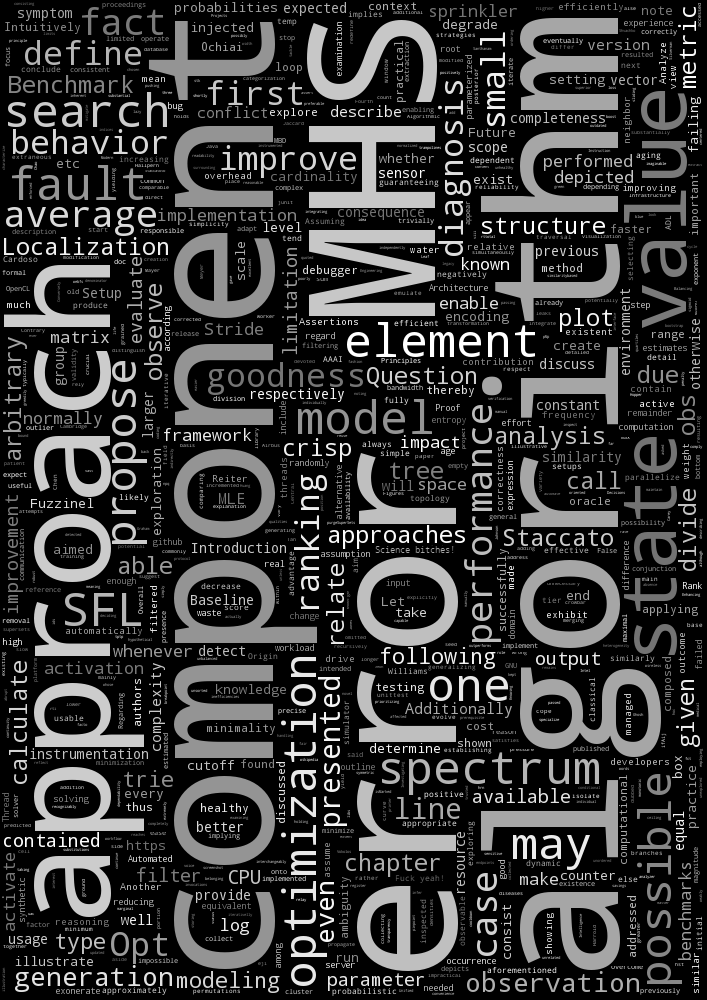
\includegraphics[width=\paperwidth]{wordcloud/wordcloud1.png}
%   };
% \end{tikzpicture}
% \fi


% \renewenvironment{dedication}
% {
%   \pagestyle{empty}% no header and footer
%   \cleardoublepage
%   \begin{flushright}

%   \vspace*{\stretch{3}}% some space at the top
%   \itshape             % the text is in italics
%   \rmfamily
%   \Large
% }
% {%
%   \par % end the paragraph
%   \vspace{\stretch{1}} % space at bottom is three times that at the top
%   \end{flushright}
% }


% \begin{dedication}
%   To Charlie, my best friend and love of my life.
% \end{dedication}



\renewcommand*{\chapterpagestyle}{empty}
%\renewcommand{\BrainFuckChapter}{
%+}{+}{+}{+}{+}{+}{+}{+}{[}{>}{+}{+}{+}{+}{>}{+}{+}{+}{+}{+}{+}{>}{+}{+}{+}{+}{+}{+}{+}{+}{>}{+}{+}{+}{+}{+}{+}{+}{+}{+}{+}{>}{+}{+}{+}{+}{+}{+}{+}{+}{+}{+}{+}{+}{<}{<}{<}{<}{<}{-}{]}{>}{>}{>}{+}{.}{>}{>}{+}{+}
%{.}{+}{+}{+}{+}{+}{+}{+}{+}{+}{+}{+}{+}{+}{+}{+}{+}{+}{.}{+}{.}{-}{-}{.}{<}{+}{+}{+}{+}{+}{+}{+}{+}{+}{+}{+}{+}{+}{+}{+}{+}{+}{.}{+}{+}{.}{>}{+}{+}{.}{[}{>}{]}{<}{[}{[}{-}{]}{<}{]}{<}{<}{-}{<}{+}{+}{-}{<}{-}{-}
%}
\chapter*{Abstract}
%\addcontentsline{toc}{chapter}{Abstract}


Abstract goes here

%%% Local Variables:
%%% mode: latex
%%% TeX-master: "../main"
%%% End:

\chapter*{Impact Statement}
This is the impact statement required by UCL, this is just to demonstrate how I laid it out.

\paragraph{Immediate academic community}
\blindtext


\paragraph{Wider academic community}
\blindtext


\paragraph{Beyond academia}
\blindtext

\acresetall
%%% Local Variables:
%%% mode: latex
%%% TeX-master: "../main"
%%% End:

\renewcommand*{\chapterpagestyle}{plain}
\cleardoublepage
\pagestyle{plain}
% \pagenumbering{roman}

\renewcommand{\BrainFuckChapter}{
}

\phantomsection
\addcontentsline{toc}{chapter}{Contents}

\tableofcontents

\renewcommand{\BrainFuckChapter}{
}
\listoffigures

\renewcommand{\BrainFuckChapter}{
}

% \listofalgorithms
% \addcontentsline{toc}{chapter}{List of Algorithms}



\chapter*{List of Acronyms}
\addcontentsline{toc}{chapter}{List of Acronyms}

\makeatletter
\patchcmd{\AC@@acro}{] #3}{] \MakeUppercase #3}{}{}
\patchcmd{\AC@@acro}{] #3}{] \MakeUppercase #3}{}{}
\makeatother
%%%%%%% ACRONYMS%%%%%%%%%%%
\begin{acronym}
  \acro{ADC}[ADC]{apparent diffusion coefficient}
  \acro{AFD}[AFD]{apparent fibre density}
  \acro{API}[API]{application program interface}
  \acro{BT}[BT]{Bloch-Torrey}
  \acro{BVH}[BVH]{bounding volume hierarchy}
  \acro{CAM}[CAM]{cell adhesion molecule}
  \acro{CC}[CC]{corpus callosum}
  \acro{CHARMED}[CHARMED]{composited hindered and restricted models of diffusion}
  \acro{ConFiG}[ConFiG]{contextual fibre growth}
  \acro{CPU}[CPU]{central processing unit}
  \acro{CSD}[CSD]{constrained spherical deconvolution}
  \acro{CUDA}[CUDA]{Compute Unified Device Architecture}
  \acro{dMRI}[dMRI]{diffusion MRI}
  \acro{DKI}[DKI]{diffusion kurtosis imaging}
  \acro{DMS}[DMS]{Diffusion Microscopist Simulator}
  \acro{DSI}[DSI]{diffusion spectrum imaging}
  \acro{DTI}[DTI]{diffusion tensor imaging}
  \acro{EM}[EM]{electron microscopy}
  \acro{ESAG}[ESAG]{elliptically symmetric angular Gaussian}
  \acro{FA}[FA]{fractional anisotropy}
  \acro{FDM}[FDM]{finite difference method}
  \acro{FEM}[FEM]{finite element method}
  \acro{FID}[FID]{free induction decay}
  \acro{FOD}[FOD]{fibre orientation distribution}
  \acro{FRF}[FRF]{fibre response function}
  \acro{GM}[GM]{grey matter}
  \acro{GPGPU}[GPGPU]{general purpose computing on graphics processing units}
  \acro{GPU}[GPU]{graphics processing unit}
  \acro{HCP}[HCP]{Human Connectome Project}
  \acro{IC}[IC]{internal capsule}
  \acro{MC}[MC]{Monte-Carlo}
  \acro{MEDUSA}[MEDUSA]{microstructure environment designer with unified sphere atoms}
  \acro{MRI}[MRI]{magnetic resonance imaging}
  \acro{MRS}[MRS]{magnetic resonance spectroscopy}
  \acro{MS}[MS]{multiple sclerosis}
  \acro{MSD}[MSD]{mean squared displacement}
  \acro{NMR}[NMR]{nuclear magnetic resonance}
  \acro{NN}[NN]{neural network}
  \acro{NODDI}[NODDI]{neurite orientation dispersion and density imaging}
  \acro{OD}[OD]{orientation dispersion}
  \acro{OGSE}[OGSE]{oscillating gradient spin echo}
  \acro{PDE}[PDE]{partial differential equation}
  \acro{PGSE}[PGSE]{pulsed gradient spin echo}
  \acro{preFiG}[preFiG]{preliminary fibre growth}
  \acro{RF}[RF]{radiofrequency}
  \acro{RWS}[RWS]{Random Walk Simulator}
  \acro{SBEM}[SBEM]{serial block-face scanning electron microscopy}
  \acro{SD}[SD]{spherical deconvolution}
  \acro{SEM}[SEM]{scanning electron microscopy}
  \acro{SGP}[SGP]{short gradient pulse}
  \acro{SH}[SH]{spherical harmonic}
  \acro{SNR}[SNR]{signal-to-noise ratio}
  \acro{TBI}[TBI]{traumatic brain injury}
  \acro{TC}[TC]{three crossing}
  \acro{TE}[TE]{echo time}
  \acro{TEM}[TEM]{transmission electron microscopy}
  \acro{WM}[WM]{white matter}
\end{acronym}


%%% Local Variables:
%%% mode: latex
%%% TeX-master: "../main"
%%% End:


\cleardoublepage

\acresetall{}
\renewcommand*{\chapterpagestyle}{scrheadings}

\pagestyle{scrheadings}
% \pagenumbering{arabic}
% \chapter{Rough Plan	}
\label{sec:plan}

\section{General idea}
Summary of all of the ConFiG work done in the PhD, split into four sections:
\begin{itemize}
\item The original ipmi implementation
\item Teh additions to make final ConFiG
\item the microstructural evalulation from the config paper
\item The FRF experiments
\end{itemize}


\section{Rough Structure}
\begin{itemize}
	\item Introduction
	\begin{itemize}
		\item General introduction to the context of the project. Why do this work, set the scene for the coming sections
	\end{itemize}
	\item Background
	\begin{itemize}
		\item Basic physics of MRI/MRS and diffusion
		\item Description of how diffusion simulation works
		\item Perhaps description of what we know about growth of fibres
	\end{itemize}
	\item Literature Review
	\begin{itemize}
		\item Simulation review that I've already done
		\item Some review of growth things, probably discuss previous white matter substrates, maybe mention space colonisation for contextual growth.
	\end{itemize}
      \item IPMI implementation
	\begin{itemize}
        \item Essentially this is just the IPMI paper with the very basic evaluation of the dMRI signals
		\end{itemize}
	  \item ConFiG
		\begin{itemize}
		\item Extra biological motivations
		\item more thorough dMRI evaluation
		\end{itemize}
	  \item Microstructural evaluation
		\begin{itemize}
		\item Microstructural eval from ConFiG paper
		\item including the new evaluation of the cross sections
		\end{itemize}
	  \item FRF experiment
		\begin{itemize}
		\item Still just working this one through
		\end{itemize}
      \item Discussion
      \item Future plans
\end{itemize}

%%% Local Variables:
%%% mode: latex
%%% TeX-master: "../main"
%%% End:


\part{Introduction and background}
\label{part:intro_background}
\renewcommand{\BrainFuckChapter}{%
  {-}{[}{-}{-}{-}{-}{-}{-}{-}{>}{+}{<}{]}{>}{.}{+}{[}{-}{-}{-}{>}{+}{<}{]}{>}{.}{+}{+}{+}{+}{+}{+}{.}{-}{-}{.}{-}{-}{-}{.}{-}{-}{-}{-}{-}{-}{-}{-}{-}{-}{-}{.}{-}{-}{[}{-}{-}{-}{>}{+}{<}{]}{>}{-}{.}{+}{[}{-}{>}{+}
  {+}{+}{<}{]}{>}{+}{.}{-}{[}{-}{-}{-}{>}{+}{<}{]}{>}{-}{-}{.}{-}{-}{-}{-}{-}{-}{-}{-}{-}{-}{-}{.}{+}{+}{+}{+}{+}{+}{.}{-}{.}{-}{>}{<}{>}{>}{+}{+}{>}{>}{+}{<}{-}{-}{>}{-}{<}{<}{+}{<}{>}{>}{+}{>}{-}{<}{<}{-}{+}{+}
  {-}{>}{-}{-}{+}{+}{<}{>}{+}{-}{<}{>}{+}{>}{<}{>}{-}{<}{>}{<}{-}{+}{-}{<}{+}{>}{>}{<}{>}{-}{-}{-}{-}{>}{>}{<}{-}{>}{+}{-}{-}{<}{<}{>}{-}{>}{-}{>}{>}{<}{<}{-}{-}{+}{<}{<}{+}{-}{<}{>}{<}{+}{+}{-}{<}{+}{<}{<}{-}{<}
}
\renewcommand{\LifeChapter}{y}
%%%%%%%%%%% Sprinkler Example Stuff%%%%%%%%%%%%%
\colorlet{grass}{clrd!80!green}

\tikzstyle{joint}=[cross out,rotate=45,line width=1 pt,draw=Black]
\tikzstyle{sensor}=[cross out,draw=Black,line width=1 pt,align=center,inner sep=0pt,minimum size=0.15cm,font=\tiny]
\tikzstyle{sprinkler}=[circle,draw=Black,line width=1.8 pt,align=center,inner sep=0pt,minimum size=0.2cm,font=\tiny]
\tikzstyle{radius}=[circle, dashed,draw=MidnightBlue,minimum size=1.5cm,line width=0.2 pt,align=center,font=\tiny]


\newenvironment{irrigationexample-perspective}{
  \begin{scope}[
    yshift=45,every node/.append style={
      yslant=0.5,xslant=-1},yslant=0.5,xslant=-1]
  }{
  \end{scope}
}

\newenvironment{irrigationexample-base}{
  \begin{irrigationexample-perspective}
    \fill[fill=grass,rounded corners=2em] (-1,-1) rectangle (3,3);
    \draw[opacity=0.1,step=1.0,black,thin] (-1,-1) grid (3,3);

  }{
  \end{irrigationexample-perspective}
}

\newenvironment{irrigationexample-sprinklers}{
  \begin{irrigationexample-base}
    \node [style=sprinkler] (s1) at (0, 2) {};
    \node [style=sprinkler] (s2) at (1, 2) {};
    \node [style=sprinkler] (s3) at (2, 2) {};
    \node [style=sprinkler] (s4) at (0, 1) {};
    \node [style=sprinkler] (s5) at (1, 1) {};
    \node [style=sprinkler] (s6) at (2, 1) {};
    \node [style=sprinkler] (s7) at (0, 0) {};
    \node [style=sprinkler] (s8) at (1, 0) {};
    \node [style=sprinkler] (s9) at (2, 0) {};
  }{
  \end{irrigationexample-base}
}

\newenvironment{irrigationexample-pipes}{
  \begin{irrigationexample-sprinklers}
    \node [style=joint] (sup) at (0, -1) {};

    \draw[thick] (s4) -- (s1) node[inner sep=0em, pos=0.5] (p1) {};
    \draw[thick] (s7) -- (s4) node[inner sep=0em, pos=0.5] (p2) {};
    \draw[thick] (sup) -- (s7)node[inner sep=0em, pos=0.5] (p3) {};
    \draw[thick] (s7) -- (s8) node[inner sep=0em, pos=0.5] (p4) {};
    \draw[thick] (s5) -- (s2) node[inner sep=0em, pos=0.5] (p5) {};
    \draw[thick] (s8) -- (s5) node[inner sep=0em, pos=0.5] (p6) {};
    \draw[thick] (s2) -- (s3) node[inner sep=0em, pos=0.5] (p7) {};
    \draw[thick] (s8) -- (s9) node[inner sep=0em, pos=0.5] (p8) {};
    \draw[thick] (s9) -- (s6) node[inner sep=0em, pos=0.5] (p9) {};
  }{
  \end{irrigationexample-sprinklers}
}


\newenvironment{irrigationexample-fuzzyerrors-continuous}{
  \begin{irrigationexample-perspective}
    \begin{scope}[transparency group]
      \clip[rounded corners=2em] (-1,-1) rectangle (3,3);
      \fill[grass,fill,rounded corners=2em] (-1,-1) rectangle (3,3);

      %\shade[shading=radial, inner color=brown, outer color=green, rounded  corners=2em] (-1,-4) rectangle (3,3);
      \fill[brown, path fading=fade out] (-1, -1) circle (6);
    \end{scope}
    \draw[opacity=0.1,step=1.0,black,thin] (-1,-1) grid (3,3);
  }{
  \end{irrigationexample-perspective}
}

\newenvironment{irrigationexample-fuzzyerrors-discrete}{
  \begin{irrigationexample-perspective}
    \begin{scope}
      \clip[rounded corners=2em] (-1,-1) rectangle (3,3);
      \fill[grass,fill,rounded corners=2em] (-1,-1) rectangle (3,3);

      \fill[brown] (-1,-1) rectangle (1,1);


    \end{scope}
    \draw[opacity=0.1,step=1.0,black,thin] (-1,-1) grid (3,3);

}{
  \end{irrigationexample-perspective}
}


\chapter{Introduction}
\label{sec:introduction}

Modern society is increasingly dependent on technology and, with the
appearance of low-cost computing environments, this dependency has
experienced an exponential growth.
%
Within a half-century span, computers evolved from a state where they
were only able to interact with nearby systems to the point where they
can communicate within a matter of seconds despite their distance
\citep{Allan01,Polsson}.
%
Furthermore, with the availability of low-cost high-speed
interconnections, software systems grew to global scales and gradually
infiltrated most aspects of the modern life style.

The rapid growth of software systems in terms of both size and number
happens mainly due to the fact that computers are an extremely
versatile tool, which can be used to more efficiently solve a large
variety of tasks in different domains.
%
One side effect of the large scope of software systems is the increase
in complexity \citep{Horn01}.
%
The rise in complexity almost unavoidably leads to a growing number of
bugs which, in turn, can eventually cause errors/failures
\citep{Salehie05}.


When unexpected behavior is observed, developers need to identify the
root cause(s) that made the system deviate from its intended behavior.
%
This task (also known as software debugging, fault localization, or
error diagnosis) is the most time-intensive and expensive phase of the
software development cycle \citep{Hailpern02}, and has been a concern
since the beginning of computer history\footnote{In 1946, the term bug
  was first used in the scope of computer science by Grace Hopper to
  document a problem in the Mark II computer.  In fact, the source of
  the problem was an actual bug (more specifically a moth) that was
  trapped in a relay, impeding its correct functioning.}.
%
In fact, it was estimated that the global cost of debugging software
has risen to \$312 billion annually\footnote{ University of
  Cambridge, "Financial content: Cambridge University study states
  software bugs cost economy \$312 billion per year",
  \url{http://www.prweb.com/releases/2013/1/prweb10298185.htm},
  accessed October 06, 2015.}.
%
To put this value into perspective, that is equivalent to the cost of
$729$ ``Airbus A380'' aircrafts\footnote{\$428 million per unit,
  \url{https://en.wikipedia.org/wiki/Airbus_A380}, accessed October
  06, 2015.}.

The high cost of debugging software is related to the fact that the
process of detecting, locating and fixing faults is both non-trivial
and error-prone.
%
It was estimated that a great share of the development resources,
easily ranging from $50\%$ to $70\%$, is normally assigned to software
testing and diagnosis \citep{Hailpern02} and that even experienced
developers are wrong almost $90\%$ of the time in their initial
guesses about the the faults' locations \citep{Ko08}.


To ease this process several diagnostic tools have been proposed (see
\Cref{ch:related-work} for examples).
%
Despite the improvement that such development-time diagnostic-related
tools represent, it remains practically impossible to create faultless
systems.
%
Acknowledging this fact, the concept of self-healing system has been
proposed.
%
Self-healing systems have the goal of improving their
dependability\footnote{According to \citep{Avizienis04}, dependability
  is an integrating concept that encompasses availability (readiness
  for correct service), reliability (continuity of correct service),
  safety (absence of catastrophic consequences on the users and the
  environment), integrity (absence of improper systems alterations)
  and maintainability (ability to undergo modifications and repairs).}
at run-time while reducing human intervention by employing mechanisms
that either prevent or solve eventual errors \citep{Ghosh07}.
%
In \citep{Psaier11}, the authors summarize the concept of self-healing
system as follows (\Cref{fig:introduction:self-healing}):
%
\vspace{-1em}
\begin{quote}
  ``The reason for enhancing a system with self-healing properties is
  to achieve continuous availability.
  %
  Compensating the dynamics of a running system, self-healing
  techniques momentarily are in charge of the maintenance of health.
  Enduring continuity includes resilience against intended, necessary
  adaptations and unintentional, arbitrary behavior.
  %
  Self-healing implementations work by detecting disruptions,
  diagnosing failure root cause and deriving a remedy, and recovering
  with a sound strategy.
  %
  Additionally, to the accuracy of the essential sensor and actuator
  infrastructure, the success depends on timely detection of system
  misbehavior.
  %
  This is only possible by continuously analyzing the sensed data as
  well as observing the results of necessary adaptation actions.
  %
  The system design leads to a control loop similar assembly.
  %
  An environment dependent and preferably adaptable set of policies
  support remedy decisions.
  %
  Possible policies include simple sets of event dependent
  instructions but also extended AI estimations supporting the
  resolution of previously unknown faults.''
\end{quote}%
\penalty10000
\vspace{-0.1em}
\begin{figure}[!ht]
  \scalebox{0.85}{
    \begin{tikzpicture}
      \tikzstyle{common}=[draw,font=\footnotesize,align=center,anchor=west,rounded
      corners=0.1cm, inner sep=0.2cm];

      \tikzstyle{sources}=[minimum width=3.5cm, common];
      \tikzstyle{props}=[minimum width=2.2cm,common];

      \tikzstyle{every node}=[sources];

      \node[fill=clrb](ac) at (0,0){Autonomic\\Computing \\ \citep{IBM06}};
      \node[fill=clrb,below = 1cm of ac](sas){Self-Adaptive\\Systems\\ \citep{Laddaga03}};
      \node[anchor=west,fill=clrb,below = 1cm of sas](fts){Fault-Tolerant\\Systems\\ \citep{Pierce65}};

      \node[fill=clrb,above right = -0.1cm and 0.5cm of fts](sss){
        Self-Stabilizing\\Systems  \\\citep{Dijkstra82}};
      \node[fill=clrb,below = 1.3cm of sss](ss){
        Survivable\\Systems \\ \citep{Linger98}};


      \tikzstyle{every node}=[common];
      \node[fill=clrb,ultra thick,fill=clra,font=\bfseries,below right= -0.6cm and 2.6cm of ac](shs){Self-Healing\\Systems};

      \draw (ac) edge[->,out=0,in=-180] (shs.west);
      \draw (sas) edge[->,out=0,in=-180]  (shs.west);
      \draw (fts) edge[->,out=0,in=-180]  (sss.west);
      \draw (fts) edge[->,out=0,in=-180]  (ss.west);
      \draw (sss) edge[->,out=30,in=-90]  (shs.south);
      \draw (ss) edge[->,out=30,in=-90] (shs.south);


      \tikzstyle{every node}=[props];


      \node[fill=clrc,above right = 0cm and 1cm of shs](vis){Vision};
      \node[fill=clrc,below = 1.25cm of vis](obj){Objectives};


      \node[fill=clrc,right = 0.7cm of vis](ca){Continuous\\Availability};
      \node[fill=clrc,below = 0.2cm of ca](mh){Maintenance\\of Health};
      \node[fill=clrc,below = 0.2cm of mh](sur){Survivability};



      \node[fill=clrc,below = 0.2cm of sur](det){Detecting};
      \node[fill=clrc,below = 0.2cm of det](dia){Diagnosing};
      \node[fill=clrc,below = 0.2cm of dia](rec){Recovery};
      \node[fill=clrc,left = of dia](att){Attributes};

      \node[fill=clrc,below = 0.2cm of rec](cl){Closed-loop};
      \node[fill=clrc,below = 0.2cm of cl](pol){Policies};
      \node[fill=clrc,below = 1.7cm of att](mea){Means};

      \draw (shs) edge[->,out=0,in=-180] (vis.west);
      \draw (shs) edge[->,out=0,in=-180] (obj.west);
      \draw (shs) edge[->,out=-60,in=180] (att.west);
      \draw (shs) edge[->,out=-60,in=140] (mea.west);


      \draw (vis) edge[->,out=0,in=-180] (ca.west);
      \draw (obj) edge[->,out=0,in=-180] (mh.west);
      \draw (obj) edge[->,out=0,in=-180] (sur.west);
      \draw (att) edge[->,out=0,in=-180] (det.west);
      \draw (att) edge[->,out=0,in=-180] (dia.west);
      \draw (att) edge[->,out=0,in=-180] (rec.west);
      \draw (mea) edge[->,out=0,in=-180] (cl.west);
      \draw (mea) edge[->,out=0,in=-180] (pol.west);

    \end{tikzpicture}
  }
  \caption{Relations and properties of self-healing research (adapted
    from \citep{Psaier11})}
  \label{fig:introduction:self-healing}
\end{figure}
\penalty-10000


The self-healing concept is in fact a specialization of a broader
concept, called autonomic computing \citep{Kephart03}.
%
To implement an autonomic system, \emph{IBM} suggests a reference
model for autonomic control loops \citep{IBM06}, referred to as the
\ac{MAPE-K} control loop and is depicted in
\Cref{fig:intro:MAPE-K-control-loop}.
%
In the \ac{MAPE-K} autonomic loop, the managed resource represents
any software or hardware resource that is given autonomic behavior by
coupling it with an autonomic manager.
%
In a practice, the managed resource can be, for instance, a web
server, a database, an operating system, a cluster of machines, a hard
drive, a wired or wireless network, \etc.

\begin{figure}[!ht]
  \includegraphics[width=0.6\columnwidth,page=13]{figures/introduction/figures/main.pdf}
  \caption{\acs{MAPE-K} control loop\label{fig:intro:MAPE-K-control-loop} }
\end{figure}




In the context of self-healing systems, the \emph{monitor} component
determines whether the system is in degraded or erroneous state,
through the information collected by the managed resource's sensors
(also known as probes or gauges \citep{Garlan01}).
%
The \emph{analyzer} component is responsible for pinpointing the
probable source(s) of system errors.
%
The \emph{plan} component creates a repair plan targeted at returning
the system to an operational state.
%
The \emph{executor} component implements the repair plan, by using a set of
system effectors that carry out changes to the managed resource.
%
The change implemented by the \emph{effectors} can be coarse-grained
(\eg, adding or removing servers to a web server cluster
\citep{Garlan04}) or fine-grained (\eg, changing configuration
parameters in a web server) \citep{Bigus02}.
%
The \emph{knowledge} component collects the knowledge produced by all
the aforementioned components and stores it for future use.



In this thesis, our focus is on the analyzer component of the
\ac{MAPE-K} control loop.
%
Our goal is to create an automatic diagnostic framework for run-time
systems.
%
Even though several diagnostic approaches have been proposed the large
majority is either too specific to a particular application (\eg,
\citep{Chao04,Mohammadi07,Kasick10,Tan10,Shvachko10}) or too costly
(\eg, \citep{Reiter87,Kleer87,Mayer03,Wotawa02}).
%
In contrast to the existent approaches, we aim at creating a
diagnostic framework meeting the following criteria:
%
\begin{itemize}[nolistsep]
\item It must be ``general purpose'':
  \begin{itemize}
  \item It must be usable in a large variety of systems.
  \item It must be possible to add new components to the managed
    resource without altering the diagnostic framework.
  \item It must handle different instrumentation granularities.
  \end{itemize}

\item It must be ``scalable'':
  \begin{itemize}
  \item It must be able to handle systems with large number of
    components.
  \end{itemize}

\item It must be ``accurate''
\end{itemize}
%

To achieve our goal while meeting the aforementioned criteria, we
improve over a development-time diagnostic technique called \ac{SFL}.
%
\ac{SFL} uses a high-level abstraction of the system under analysis,
making it, in principle, usable in a large diversity of scenarios.
%
The only requirements to use \ac{SFL} in a real-world scenario are
that
\begin{inparaenum}[(1)]
\item the system's activity must be divisible into transactions,
\item the correctness of each transaction must be evaluable,
\item the components' activations must be observable and
\item it must be possible to associate the components' activity with
  the corresponding transactions.
\end{inparaenum}

The high-level abstraction implies that a large amount of the
diagnostic complexity is traded-off for accuracy.
%
Even though \ac{SFL} is less accurate than some existing diagnostic
approaches (\eg, \citep{Reiter87,Kleer87,Mayer03,Wotawa02}), it is able to
scale to large systems where heavier approaches are not usable.
%
Furthermore, given enough diversity in the observations, \ac{SFL}
tends to be accurate enough for practical
purposes \citep{Santelices09,Abreu09f}.


In the remainder of this chapter we further discuss the scope of our
work.
%
In \CrefPageParen{sec:intro:diagnostic-problem}, we describe the
diagnostic problem.
%
In \CrefPageParen{sec:intro:SFL}, we present the state-of-the-art
\ac{SFL} approach for development-time diagnosis.
%
In \CrefPageParen{sec:intro:research-goals}, we discuss our research
goals.
%
In \CrefPageParen{sec:intro:origin-of-chapters}, we present the origin of
chapters.
%
Finally, in \CrefPageParen{sec:intro:outline}, we present the thesis
outline.

\section{Diagnostic Problem}
\label{sec:intro:diagnostic-problem}
In general terms, a diagnostic problem occurs whenever the behavior of
a particular system (natural or artificial) deviates from the expected
behavior \citep{Reiter87,Kleer92}.
%
The challenge consists in finding the true root causes of such
abnormal behavior.
%

In our work we use the taxonomy proposed by \citep{Avizienis04}:
\begin{itemize}
\item An \textbf{error} is an incorrect system state that may cause a
  failure.
\item A \textbf{failure}, is the observable manifestation of an error:
  an error becomes a failure when it propagates to the system's output.
\item A \textbf{fault/bug} is the cause of an error in the system.
\end{itemize}

\begin{figure}[h!]
  \lstinputlisting[
  language=python,
  xleftmargin=.1\textwidth,
  xrightmargin=.1\textwidth,
  ]{figures/introduction/error.py}
  \caption{Bug example\label{fig:bugexample}}
\end{figure}

To illustrate these concepts, take for instance the three Python
functions presented in \Cref{fig:bugexample}.
%
The purpose of function $\fn{f\_to\_c}$ is to convert a temperature
from \textit{Fahrenheit} degrees to \textit{Celsius}.
%
Since the whole operation is performed using integer arithmetic, the
implementation is faulty and may compute erroneous results.
%
Function $\fn{is\_freezing\_f}$, which is implemented by daisy
chaining functions $\fn{f\_to\_c}$ and $\fn{is\_freezing\_c}$, should
return $\mTrue$ if the input value (in \textit{Fahrenheit}) is
below water's freezing point and $\mFalse$ otherwise.

\begin{figure}[!ht]
  \begin{tabular}{c|r@{}@{}lr@{}l|cc|c}
    % \cline{2-7}
    \multicolumn{1}{c|}{} & \multicolumn{4}{c|}{$\fn{f\_to\_c}$} & \multicolumn{2}{c|}{$\fn{is\_freezing\_f}$}                                                           \\
    \hline
    Input                 & \multicolumn{2}{c}{Expected}         & \multicolumn{2}{c|}{Observed} & Expected & Observed    & Outcome                                      \\
    \hline
    $31^{\circ} F$        & $-0.55_{5}$                          & $^{\circ}C$                   & $-1$     & $^{\circ}C$ & $\mTrue$  & $\mTrue$ & Error   \\
    $32^{\circ} F$        & $0$                                  & $^{\circ}C$                   & $0$      & $^{\circ}C$ & $\mTrue$  & $\mTrue$ & Nominal \\
    $33^{\circ} F$        & $0.55_{5}$                           & $^{\circ}C$                   & $0$      & $^{\circ}C$ & $\mFalse$ & $\mTrue$ & Failure \\
  \end{tabular}

  \caption{$\fn{is\_freezing\_f}$ function trace\label{tab:trace}}
\end{figure}
By analyzing \Cref{tab:trace}, we can see that for $32^\circ F$ the
function \textit{$\fn{is\_freezing\_f}$} not only works as expected
but also does not activate the fault (\ie, the result of
$\fn{f\_to\_c}$ is correct).
%
For $31^\circ F$, despite activating the fault (\ie, the result of
$\fn{f\_to\_c}$ is not correct), the aggregate result of both
functions is correct due to the fact that function
$\fn{is\_freezing\_c}$ masks the error.
%
Finally, for $33^\circ F$ the fault is activated and the error
propagates to the system output, delivering an incorrect result.

A prerequisite to diagnose a system is that the occurrence of
errors/failures is detected.
%
The process of observing the system state and deciding whether or not
it satisfies the system's specification is known as the oracle
problem.


The approaches to solve the diagnostic problem can be broadly divided
in two groups: heuristic and model based diagnosis (also known as
diagnosis from first principles).

\subsection{Heuristic-based Diagnosis}
\label{sec:intro:heuristic-diagnosis}
Heuristic-based diagnosis approaches are focused on encoding expert
knowledge generated by previous diagnostic experience to more
efficiently address future diagnostic problems.
%
In such diagnostic systems, the diagnostic reasoning is greatly based
upon the observed error symptoms and the possible (known) solutions to
such symptoms.
%
A consequence of this type of reasoning is that the structure of the
system under analysis is only weakly represented, if present at all.
%
While such diagnostic systems are effective in diagnosing known
abnormalities, they tend to fail whenever new error symptoms emerge.

\begin{figure}[ht]
  \begin{subfigure}{\columnwidth}
    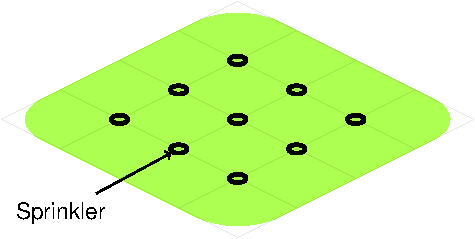
\includegraphics[page=1]{figures/introduction/figures/main.pdf}
    \caption{Sprinklers\label{fig:intro:irrigation-example-sprinklers}}
  \end{subfigure}


  \begin{subfigure}{\columnwidth}
    \includegraphics[page=2]{figures/introduction/figures/main.pdf}
    \caption{Piping\label{fig:intro:irrigation-example-piping}}
  \end{subfigure}
  \caption{Irrigation system example\label{fig:intro:irrigation-example}}
\end{figure}

As an illustrative example, consider an irrigation system with the
additional goal of guaranteeing that irrigation problems are
automatically detected and diagnosed.
%
For the example shown in
\Cref{fig:intro:irrigation-example-sprinklers}, one could use
peer-similarity to accomplish the self-diagnosis goal.
%
The usage of peer-similarity requires that all
components in the system behave similarly with regard to a set of
metrics and the presence of outlier metric values implies the
occurrence of errors in the corresponding components
\citep{Kasick10,Shvachko10,Tan10}.
%
Assuming that, for instance, the water pressure or consumption for
each sprinkler is observable, substantial variations in such metrics
among the system's sprinklers would signal a sprinkler failure.


Even though this approach would most likely perform well in the
described system, in a system where the sprinklers operate at
different pressures or have different water consumption rates the
outlier detection would be too inaccurate.
%
Furthermore, if all the sprinklers in the system fail similarly, this
particular approach may fail to detect and, consequently, to diagnose
the errors.

Another problem with the aforementioned approach is related to the
fact that, to meet the similarity requirement, the abstraction of the
system neglects the existence of important components and may result
in poor diagnostic quality.
%
Considering the fact that the sprinklers are fed by a piping system,
as depicted in \Cref{fig:intro:irrigation-example-piping}, the
observation of an error symptom in a sprinkler does not necessarily
mean that the problem occurred there.
%
In practice, the symptom of low water pressure may be due to water
shortage, piping failure, and/or sprinkler failure.

Finally, consider a situation in which the state of the sprinklers is
not directly observable but instead the system is equipped with
humidity sensors, placed at arbitrary positions in the field, as shown
in \Cref{fig:intro:example2}.
%
As the state of the system's components is not available, the
peer-similarity technique is no longer usable.


\begin{figure}[ht]
  \includegraphics[page=3]{figures/introduction/figures/main.pdf}
  \caption{Irrigation system example -- Sensors\label{fig:intro:example2}}
\end{figure}

Another example of this type of diagnostic approach is the so-called
medical diagnostic guidelines.
%
Even though such guidelines effectively enhance both diagnostic
accuracy and efficiency for common diseases, they fail in the presence
of unknown symptoms/diseases (\eg, a patient with a green glowing
eye).

Even though apparently unrelated to the computer science domain, the
previous examples show the potential problems related to heuristic
diagnostic techniques.
%
Establishing a parallel with software, we see that software systems
are mostly composed of heterogeneous sets of components with, almost
inevitably, different degrees of state observability thus strongly
limiting the scope of application of existing diagnostic heuristics
over different systems \citep{Salehie05}.

\subsection{\acl{MBD}}
\label{sec:intro:model-based-diagnosis}
\ac{MBD} approaches focus on encoding the structure and expected
behavior of the system under analysis which, together with
observations of the system's behavior, are used to perform the
diagnostic reasoning \citep{Kleer87,Reiter87}.
%
\begin{definition}[Model-based Diagnostic System]
  A model-based diagnostic system $\DS$ is defined as the triple
  $\DS = (\SD, \COMPS,\OBS)$ , where:
  \begin{itemize}
  \item $\SD$ is a propositional theory describing the behavior of the system
  \item $\COMPS = \set{c_1 , \ldots, c_M }$ is a set of components in $\SD$
  \item $\OBS$ is a set of observable variables in $\SD$
  \end{itemize}
\end{definition}


The existence of such a model enables the diagnostic system to
successfully cope (from a theoretical point-of-view) with new error
symptoms (such as the patient with the glowing eye).
%
Whenever the observed system behavior for a particular scenario (\ie,
a specific assignment over variables in $OBS$) conflicts with the
behavior predicted by the model $SD$, the diagnostic reasoning
revolves around finding sets of components that, by assuming their
faultiness, would explain the erroneous behavior.

To guarantee generality, \ac{MBD} algorithms reason in terms of
conflicts.
%
Informally, a conflict represents a set of components that cannot be
simultaneously healthy to explain the observed erroneous behavior.

\begin{definition}[h-literal]
  An h-literal, denotes the component's health.
  %
  The positive h-literal $h$ corresponds to a healthy component
  whereas, the negative h-literal $\neg h$ corresponds to an
  unhealthy one.
\end{definition}

\begin{definition}[Conflict]
  Let $\fn{HL}^+(C) = \bigwedge_{j \in C} h_j$ be the conjunction of
  positive h-literals for a set of components $C \subseteq \COMPS$ and
  $obs$ an observation term over variables in $\OBS$.  $C$ is a
  conflict for $(\DS, obs)$ if and only if:
  \begin{equation}
    \SD \wedge obs \wedge \fn{HL}^+(C)
  \end{equation}
  is inconsistent.
\end{definition}

In other words, a conflict is a set of components that cannot be
simultaneously healthy for the observed erroneous behavior
to occur.

\begin{definition}[Diagnostic Candidate]
  \label{def:intro:candidate}
  Let $C \subseteq \COMPS$ be a set of components.  We define $d(C)$
  to be the conjunction:
  \begin{equation}
    \Big(\bigwedge_{m \in C} \neg h_m\Big) \wedge
    \Big(\bigwedge_{m \in \COMPS \setminus C}  h_m\Big)
  \end{equation}
  Given an observation term $obs$ over variables in $\OBS$, a
  diagnostic candidate for $\DS$ is a conjunction $d(C)$
  such that:
  \begin{equation}
    \SD \wedge obs \wedge d(C)
  \end{equation}
  is consistent.

  In the remainder we refer to $d(C)$ simply as $d$, which
  we identify with the set $C$.
\end{definition}

In this context, a diagnostic candidate is thereby a set of components
that is conjectured to be unhealthy, resolving all conflicts entailed
by $\SD \wedge obs$.


A problem with the above definition is related to the fact that a
candidate $d$ containing all of the system's components (\ie, $d =
\COMPS$) always resolves every conflict by $\SD \wedge obs$.
%
Intuitively, this is equivalent to saying that the whole system is
faulty which, in practice, is not a very helpful conclusion.
%
To apply the concept of a diagnostic candidate to real systems with
success, one must refine the definition so that the candidate contains
the minimum number of components while still solving all the
conflicts.

\begin{definition}[Minimal Diagnostic Candidate]
  \label{def:intro:minimal-candidate}
  A candidate $d$ is minimal if and only if
  $\nexists_{d^\prime} : d^\prime \subset d$ such that $d^\prime$ is a diagnostic
  candidate.
\end{definition}

The end result of the diagnostic reasoning is the diagnostic
report.
%
A diagnostic report features a set of explanations for the erroneous
behavior (\ie, the diagnostic candidates) as well as a measure of how
likely each explanation is.
%
The process of calculating a diagnostic report can be broadly divided
in two stages, as depicted in \Cref{fig:intro:diagnostic-process}.

\begin{figure}[ht]
  \includegraphics[page=4]{figures/introduction/figures/main.pdf}
  \caption{Diagnostic process\label{fig:intro:diagnostic-process}}
\end{figure}

\begin{definition}[Diagnostic Report]
  \label{def:intro:diagnostic-report}

  A diagnostic report
  $\diag = \left(d_1, \dots, d_k, \dots, d_K\right)$ is an ordered set
  of $K$ diagnostic candidates, such that:
  \begin{equation}
    \forall_{d_k\in \diag} : \pr{d_k \mid obs} \geq \pr{d_{k+1} \mid obs}
  \end{equation}
\end{definition}


\section{\acl{SFL}}
\label{sec:intro:SFL}
A limitation of traditional \ac{MBD} approaches is the necessity of a
detailed system model which, in practice and due to the large
complexity of modern computer systems, normally entails a large
modeling effort/cost, thus narrowing its range of application
\citep{Pietersma06,Horn01}.
%
To overcome the complexity of creating precise system models,
\acf{SFL}\footnote{For simplicity and unless stated otherwise, we use
  the acronym \ac{SFL} to refer to a particular \ac{SFL} approach
  known as Spectrum-based Reasoning for Fault Localization.
  %
  In \CrefPageParen{sec:related-work:similarity-based-SFL} an
  alternative and more common \ac{SFL} approach is presented.}
approaches were proposed \citep{Abreu09a,Kleer09,Casanova13}.
%
Instead of relying on a fine grained model of the system (\ie,
$SD \in DS$) to generate conflict sets, \ac{SFL} infer conflicts by
performing a dynamic analysis of the system.

To apply \ac{SFL} to a system, it must be abstracted in terms of two
general concepts: component, and transaction.
%
A component is an element of the system that, for diagnostic purposes,
is considered to be atomic\footnote{In a software environment, a
  component can be for instance a statement, a function, a class, a
  service, \etc.}.
%
A transaction is a set of component activations that
\begin{inparaenum}[(1)]
\item share a common goal, and
\item the correctness of the provided service can be verified.
\end{inparaenum}
%
The error detection mechanism, from a \ac{SFL} perspective, is treated
as a black box.

To gather all the required information to perform diagnosis, the
system under analysis must be instrumented (see
\Cref{sec:related-work:code-coverage}).
%
The instrumentation's output, commonly known as
spectrum \citep{Harrold98}, is defined as the
pair $(A, e)$ (\Cref{fig:intro:sfl-matrix}), where:

\begin{itemize}
\item $A$ (\textbf{activity matrix}) encodes the involvement of
  components in transactions.
\item $e$ (\textbf{error vector}) encodes the correctness of each
  individual transaction.
\end{itemize}

\begin{figure}[!ht]
  \begin{equation*}
    \stackrel{\mbox{activity matrix}}{%
      \begin{bmatrix}
        A_{11} & A_{12} & \cdots & A_{1M} \\
        A_{21} & A_{22} & \cdots & A_{2M} \\
        \vdots & \vdots & \ddots & \vdots \\
        A_{N1} & A_{N2} & \cdots & A_{NM}
      \end{bmatrix}
    }\ \ \ \stackrel{\stackrel{\mbox{error}}{\mbox{vector}}}{%
      \begin{bmatrix}
        e_1    \\
        e_2    \\
        \vdots \\
        e_N
      \end{bmatrix}%
    }
  \end{equation*}
  \caption{Spectrum with $M$ components and $N$ transactions\label{fig:intro:sfl-matrix}}
\end{figure}

Even though several types of spectra exist, the most commonly used is
called a hit spectrum \citep{Harrold98,Yilmaz08,Santelices09}.
%
\begin{definition}[Hit Spectrum]
  \label{def:intro:hit-spectrum}
  The hit spectrum abstraction encodes the components' activity in terms
  of hit/not hit and the transactions' correctness in terms of
  pass/fail.
  %
  Using the hit spectrum abstraction, $A$ and $e$ are defined as:
  \begin{equation}
    A_{ij} = \begin{cases}
      1, & \textrm{if component $j$ was involved in transaction $i$}\\
      0, & \textrm{otherwise}
    \end{cases}
  \end{equation}
  \begin{equation}
    e_{i} = \begin{cases}
      1, & \textrm{if transaction $i$ failed}\\
      0, & \textrm{otherwise}
    \end{cases}
  \end{equation}
\end{definition}

For convenience, in this thesis we may treat $A_i$ as a set containing
the indices of all components involved in transaction $i$.
%
Formally, $A_i$ can also be defined as:
\begin{equation}
  A_{i} = \set{j \mid \textrm{if component $j$ was involved in transaction $i$}}
\end{equation}
%
Since both forms encode the same information, we can use the two forms
interchangeably.
%
Whenever we apply set operations to $A$, we are implicitly using the
set form.
%
In \Cref{fig:intro:hit-spectrum-example} an example hit
spectrum in both forms is presented.
\begin{figure}[ht]
  \begin{subfigure}{0.4\columnwidth}
    \begin{tabular}{c|ccc|c}
      \multirow{2}{*}{$i$} & \multicolumn{3}{c|}{$A$} & \multirow{2}{*}{$e$} \\
      \cline{2-4}
                           & $c_1$                    & $c_2$ & $c_3$ &      \\ \hline
      $1$                  & $1$                      & $1$   & $0$   & $1$  \\
      $2$                  & $1$                      & $0$   & $1$   & $1$  \\
      $3$                  & $1$                      & $1$   & $1$   & $0$  \\
    \end{tabular}
    \caption{Matrix form}
  \end{subfigure}
  \begin{subfigure}{0.4\columnwidth}
    \begin{tabular}{c|c|c}
      $i$                  & $A$                      & $e$                  \\\hline
      $1$                  & $\set{1,2}$              & $1$                  \\
      $2$                  & $\set{1,3}$              & $1$                  \\
      $3$                  & $\set{1,2,3}$            & $0$                  \\
    \end{tabular}
    \caption{Set form}
  \end{subfigure}
  \caption{Hit spectrum example\label{fig:intro:hit-spectrum-example}}
\end{figure}


\begin{figure}[!ht]
  \begin{subfigure}{\columnwidth}
    \includegraphics[page=5]{figures/introduction/figures/main.pdf}
    \caption{Components\label{fig:intro:example-sfl-components}}
  \end{subfigure}
  \\[2em]
  \begin{subfigure}{\columnwidth}
    \includegraphics[page=6]{figures/introduction/figures/main.pdf}
    \caption{Transaction\label{fig:intro:example-sfl-transaction}}
  \end{subfigure}
  \\[2em]
  \begin{subfigure}{\columnwidth}
    \bgroup
    \def\x{{\Large$\bullet$}}
    \setlength\tabcolsep{0.2em}
    \newcolumntype{T}{t{1.4em}}

    \begin{tabular}{T|TTTTTTTTTTTTTTTTTTT|T}
      \multirow{2}{*}{$i$} & \multicolumn{19}{c|}{$A$} & \multirow{2}{*}{$e$}                                                                                                                                                              \\\cline{2-20}
                           & $c_1$                     & $c_2$ & $c_3$ & $c_4$ & $c_5$ & $c_6$ & $c_7$ & $c_8$ & $c_9$ & $c_{10}$ & $c_{11}$ & $c_{12}$ & $c_{13}$ & $c_{14}$ & $c_{15}$ & $c_{16}$ & $c_{17}$ & $c_{18}$ & $c_{19}$ &     \\ \hline
      $1$                  & \hit                      & \hit  & \nhit & \hit  & \hit  & \nhit & \nhit & \nhit & \nhit & \hit     & \hit     & \hit     & \hit     & \hit     & \hit     & \nhit    & \nhit    & \nhit    & \hit     & \hit \\
      $2$                  & \nhit                     & \hit  & \hit  & \nhit & \hit  & \hit  & \nhit & \nhit & \nhit & \nhit    & \nhit    & \hit     & \hit     & \hit     & \hit     & \hit     & \hit     & \hit     & \hit     & \nhit \\
      $3$                  & \nhit                     & \nhit & \nhit & \hit  & \hit  & \nhit & \hit  & \hit  & \nhit & \nhit    & \hit     & \hit     & \hit     & \nhit    & \hit     & \nhit    & \nhit    & \nhit    & \hit     & \nhit \\
      $4$                  & \nhit                     & \nhit & \nhit & \nhit & \hit  & \hit  & \nhit & \hit  & \hit  & \nhit    & \nhit    & \hit     & \hit     & \nhit    & \hit     & \nhit    & \hit     & \hit     & \hit     & \hit \\
    \end{tabular}
    \egroup
    \caption{Hit spectrum (0's and 1's were replaced by ``.'' and
      ``{\Large$\bullet$}'' for
      readability)\label{fig:intro:example-sfl-spectrum}}
  \end{subfigure}
  \caption{Irrigation system example -- \acs{SFL}}
\end{figure}


To illustrate how \ac{SFL} can be used in an arbitrary system,
consider again the example in \Cref{fig:intro:example2}.
%
For this system, the set of all components is composed of $19$ elements
(\Cref{fig:intro:example-sfl-components}): $9$ sprinklers ($c_1$ through
$c_9$), $9$ piping elements ($c_{10}$ through $c_{18}$) and the water supply
($c_{19}$).
%
There are $4$ different transaction types (one for each
sensor).
%
Each of those transactions consists of the activation of all the
surrounding sprinklers as well as the piping elements used to by those
sprinklers, as depicted in \Cref{fig:intro:example-sfl-transaction}.
%
A possible approach to evaluate the success of each transaction would
be to compare the humidity value obtained by the corresponding sensor
to an arbitrary threshold interval.
%
If the humidity on the ground is either too high or too low,
the transaction fails.

Consider a scenario where, for the described system, sensors $s_1$ and
$s_4$ (see \Cref{fig:intro:example-sfl-transaction}) detect an incorrect
humidity level whereas, the remaining sensors, detect a corrected
humidity level.
%
The spectrum corresponding to this scenario is depicted in
\Cref{fig:intro:example-sfl-spectrum}.
%
The spectrum contains $4$ transactions (each transaction $i$
corresponds to the sensor $s_i$) and both transactions $1$ and $4$ are
marked as erroneous.
%
Additionally, for each transaction, all the sprinklers adjacent to the
corresponding sensor as well as the piping elements needed to feed
such sprinklers are marked as active.



In the next sub-sections we present the relevant details of existent
\ac{SFL} algorithms to solve both the candidate generation and ranking
problems.


\subsection{Candidate Generation}
\label{sec:intro:candidate-generation}
In a na\"{i}ve approach, the candidate generation problem can be
addressed by computing the power set of all components in the system
($\powSet{\COMPS}$).
%
However, as $|\set{\powSet{\COMPS}}| = 2^{\set{|\COMPS|}}$, this
approach becomes quickly ineffective.
%
In practice, rather than iterating over \emph{all} possible sets just
to find that most are not minimal or even consistent with the
observations, search algorithms are typically used to only consider
sets that meet the minimal candidate criteria (see
\Cref{def:intro:minimal-candidate}).
%

Despite the advantage of only computing minimal candidates, the
problem is still remarkably hard.
%
The calculation of minimal candidates, conceptually referred to as
hitting sets, is a problem equivalent to the \acl{MHS} problem
\citep{Reiter87}, which is known to be NP-Hard \citep{Garey90}.
%
The formal definition of the \acl{MHS} problem goes as follows:

\begin{definition}[Hitting Set]
  \label{def:intro:hitting-set}
  Given a set $U$ of $M$ elements (called the universe) and a
  collection $S$ of $N$ sets, a set $d$ is said to be a \acf{HS} of
  $(U,S)$ if and only if:
  \begin{equation}
    \label{eq:intro:hitting-set}
    \displaystyle \HS(U,S,d):= d \subseteq U \wedge \big(\forall_{s \in S}: d \cap s \not = \emptyset\big)
  \end{equation}
\end{definition}
\begin{corollary}
  If $\nexists_{s \in S} : s \cap U = \emptyset$, $U$ is a \ac{HS} of $S$.
\end{corollary}

\begin{corollary}
  \label{cor:intro:unsatisfiablity}
  If $\exists_{s \in S} : s \cap U = \emptyset$, $\HS(U,S,d)$ never holds.
\end{corollary}

\begin{corollary}
  \label{cor:intro:emptyHS}
  $d = \emptyset$ is a hitting for $S = \emptyset$.
\end{corollary}

\begin{corollary}
  \label{cor:intro:associativity}
  $\HS(U,S,d)$ is associative:
  \begin{equation}
    \displaystyle \HS(U,S,d) \wedge \HS(U^\prime,S^\prime,d^\prime) \implies
    \HS(U\cup U^\prime,S \cup S^\prime, d \cup d^\prime)
  \end{equation}
\end{corollary}

\begin{definition}[Minimal Hitting Set]
  A set $d$ is a \acf{MHS} of $(U,S)$ if and only if:
  \begin{equation}
    \label{eq:intro:minimal-hitting-set}
    \MHS(U,S,d):= \HS(U,S,d) \wedge \big(\nexists_{d^\prime \subset d}: \HS(U,S,d^\prime)\big)
  \end{equation}
  \noindent
  \ie, $d$ is a \ac{HS} and no proper subset of $d$ is a \ac{HS}.
\end{definition}
%
There may be several \acp{MHS} $d_k$ for $(U,S)$, which
constitute the \ac{MHS} collection $D$.
%
The \ac{MHS} problem consists thereby in computing $D$ for a
particular pair $(U,S)$.

Putting this definition in terms of the candidate generation problem,
the set of all components of the system ($\COMPS$) is equivalent to
the set $U$, whereas the set of all conflicts entailed by
$\SD \wedge obs$ is equivalent to $S$.
%
A \ac{MHS} for all the conflicts entailed by $\SD \wedge obs$ is, in
fact, a diagnostic candidate for $\SD \wedge obs$ \citep{Reiter87}.


Under the \ac{SFL} abstraction, a conflict occurs whenever a failed
transaction exists in the spectrum.
%
The elements of the conflict set are the components activated in such
transaction.
%
Intuitively, since the transaction failed, it follows that at least
one of the components must not be healthy for the erroneous behavior
to occur.


As an example, consider the hit spectrum in
\Cref{fig:intro:spectrum-example} for which all $2^M$ possible (but
not necessarily valid) candidates (\ie, $\powSet{\COMPS}$) are
presented in \Cref{fig:intro:hasse}.
%
For this particular spectrum, two minimal candidates/\acp{MHS} exist:
$\set{1}$ and $\set{2,3}$.
%
Even though the set $\set{1,2,3}$ is also \ac{HS}, it is not minimal
as it can be subsumed either by $\set{1}$ or $\set{2,3}$.

\begin{figure}[ht]
  \begin{subfigure}{0.4\columnwidth}
    \begin{tabular}{c|c|c}
      $i$ & $A$           & $e$ \\\hline
      $1$ & $\set{1,2}$   & $1$ \\
      $2$ & $\set{1,3}$   & $1$ \\
      $3$ & $\set{1,2,3}$ & $0$ \\
    \end{tabular}
    \caption{Hit spectrum\label{fig:intro:spectrum-example}}
  \end{subfigure}
  %
  \begin{subfigure}{0.45\columnwidth}
    \includegraphics[page=7]{figures/introduction/figures/main.pdf}
    \caption{Hasse diagram of $\powSet{\set{1,2,3}}$\label{fig:intro:hasse}}
  \end{subfigure}
  \caption{Example}
\end{figure}





Being a NP-hard problem, the usage of exhaustive search algorithms
(\eg, \citep{Reiter87,Wotawa01}), is prohibitive for most real-world
problems.
%
In order to solve the candidate generation problem in a reasonable
amount of time, approaches that relax the strict
minimality\footnote{We use the term minimal in a more liberal way due
  to mentioned relaxation. A candidate $d$ is said to be minimal if no
  other calculated candidate is contained in $d$.} constraint have
been proposed \citep{Abreu09b,Kleer92,Feldman08}.

A simplified\footnote{For simplicity, the cutoff conditions were
  omitted.} version of the state-of-the-art \ac{SFL} candidate
generation algorithm (called \staccato{}) \citep{Abreu09b} is
presented in \Cref{alg:intro:staccato} and
\Cref{fig:intro:cg-flowchart}.
%
The algorithm works in a divide and conquer fashion by, at each stage
of its execution, performing one of two different tasks (lines
\ref{alg:intro:staccato:rank},
\ref{alg:intro:staccato:S'}, and
\ref{alg:intro:staccato:rec} or
\ref{alg:intro:staccato:isminimal}--\ref{alg:intro:staccato:addD}),
depending on whether the set $d$ is a \ac{HS}.
%
As we shall shortly see, due to the algorithm's divide and conquer
nature, $d$ is a \ac{HS} whenever $S = \emptyset$.

The first task, which is triggered whenever $d$ is not a \ac{HS} (line
\ref{alg:intro:staccato:divide}), aims at dividing the initial
problem in smaller sub-problems.
%
This goal is achieved by iteratively selecting an element $j \in U$
from a heuristically\footnote{The details of chosen heuristic are
  presented in \Cref{sec:mhs2o:heuristics}. For now assume that the
  order is arbitrary and that, for every possible ordering, the
  algorithm computes the same result.} ordered set (line
\ref{alg:intro:staccato:rank}) and creating a temporary collection
$S^\prime$
containing all the sets $s \in S : j \in s$,
\ie, the sets hit by $\set{j}$ (line \ref{alg:intro:staccato:S'}).
%
Finally, the algorithm makes a recursive call to solve the sub-problem
$S \setminus S^\prime$ with set $d \cup \{j\}$ (line
\ref{alg:intro:staccato:rec}).

The second task, which occurs whenever $d$ is a \ac{HS} (line
\ref{alg:intro:staccato:conquer}), aims at collecting \acp{HS}
while guaranteeing that no \ac{HS} in $D$ has a proper subset also
contained in $D$.
%
The first step in this task is to check if $d$ is minimal (line
\ref{alg:intro:staccato:isminimal}) with regard to the already
discovered \ac{MHS} collection $D$.
%
If $d$ is minimal, all super-sets of $d$ in $D$ are purged (line
\ref{alg:intro:staccato:purge}) and, finally, $d$ is added to
$D$ (line \ref{alg:intro:staccato:addD}).

\begin{algorithm}
  \begin{description}
  \item[Inputs:]\ $(U, S, d=\emptyset, D=\emptyset)$
  \item[Output:]\ Minimal hitting set collection $D$
  \end{description}

  \begin{algorithmic}[1]
    \If{$S \not= \emptyset$}   \algorithmiccomment{\textbf{divide task}} \label{alg:intro:staccato:divide}
    \For{$j \in  \fn{Rank}(U, S)$} \label{alg:intro:staccato:rank}
    \State $S^\prime \gets \set{s \mid s \in S \wedge j \in s}$  \label{alg:intro:staccato:S'}
    \State $D \gets \fn{Staccato}(U \setminus \set{j}, S \setminus S^\prime, d \cup \set{j}, D)$  \label{alg:intro:staccato:rec}
    \EndFor
    \Else
    \algorithmiccomment{\textbf{conquer task}} \label{alg:intro:staccato:conquer}
    \If{$\nexists_{d^\prime\in D}: d^\prime\subseteq d$} \label{alg:intro:staccato:isminimal}
    \State $D \gets D \setminus \set{d^\prime \mid d^\prime \in D \wedge  d \subseteq d^\prime}$  \label{alg:intro:staccato:purge}
    \State $D \gets D \cup \set{d}$ \label{alg:intro:staccato:addD}
    \EndIf
    \EndIf
    \State \Return $D$
  \end{algorithmic}
  \caption{\staccato{}\label{alg:intro:staccato}}
\end{algorithm}

\begin{figure}[!ht]
  \includegraphics[scale=0.9,page=14]{figures/introduction/figures/main.pdf}
  \caption{Candidate generation flowchart\label{fig:intro:cg-flowchart} }
\end{figure}


\begin{figure}[!ht]
  \includegraphics[page=8]{figures/introduction/figures/main.pdf}
  \caption{Example search tree (pre-order traversal, from top to bottom)}
  \label{fig:intro:staccato-search-tree}
\end{figure}


To illustrate how \staccato{} works, consider the example in
\Cref{fig:intro:staccato-search-tree}\footnote{Note that the order of
  node exploration (and consequently the shape of the tree) was
  selected for illustrative purposes.} which represents a possible
search tree for \staccato{} with $U = \set{1,2,3}$ and $S =
\set{\set{1,2}, \set{1,3}}$ (\Cref{fig:intro:spectrum-example}).
%
Each node in the search tree represents a call to the function (all
the parameters as well as the return value are encoded as a table).
%
Leaf nodes represent function calls for which $d$ is a \ac{HS} whereas
intermediate nodes represent calls for which $d$ is not a \ac{HS}.


In the outer call to the algorithm (the leftmost node), as
$S \not= \emptyset$, the algorithm performs the divide task.
%
After exploring the sub-tree starting with $d=\{2\}$,
the algorithm yields the collection $D=\{\{1,2\},\{2,3\}\}$.

We can see that at this point, if the execution were to be
interrupted, $\{1,2\}$ would be erroneously considered a \ac{MHS}.
%
However, after exploring the sub-tree starting with $d = \{1\}$,
the set $\{1,2\}$
is removed yielding the collection $D=\{\{1\},\{2,3\}\}$.

The inspection of the sub-tree starting with $d = \{3\}$
does not make further changes to collection $D$.
%
On the one hand, the \ac{HS} $\{1,3\}$ is a proper super-set of
$\{1\}$.
%
On the other hand, the \ac{HS} $\{2,3\}$ is already contained in
$D$.
%

As expected, the result for this example would be the collection
$D=\{\{1\},\{2,3\}\}$.
%
\FloatBarrier
\subsection{Candidate Ranking}
\label{sec:intro:candidate-ranking}
The candidate ranking problem is normally addressed using a na\"{i}ve
Bayes classifier \citep{Abreu09a,Kleer09}.
%
Concretely, the posterior probability of each candidate $d \in D$
given the observed run-time behavior ($\pr{d \mid obs}$) is calculated
assuming conditional independence throughout the process
(\Cref{fig:intro:cr-flowchart}).

\begin{figure}[!ht]
  \includegraphics[scale=0.9,page=15]{figures/introduction/figures/main.pdf}
  \caption{Candidate ranking flowchart\label{fig:intro:cr-flowchart}}
\end{figure}


Under a set of observations, the posterior probabilities are
calculated according to Bayes rule as:
%
\begin{equation}
  \pr{d\mid obs} = \pr{d} \times \frac{\pr{obs\mid d}}{\pr{obs}}
\end{equation}

Since for \ac{SFL} $obs = (A,e)$, we can rewrite the previous
expression as:
\begin{equation}
  \begin{split}
    \posterior{}   & =  \pr{d} \times \frac{\displaystyle \likelihood}{\pr{A, e}} \\
    & =  \pr{d} \times\frac{\displaystyle \prod_{i \in 1..N} \likelihoodi}{\pr{A, e}}
  \end{split}
\end{equation}


%
The denominator $\pr{A, e}$ is a normalizing term that is identical
for all $d \in D$ and is not considered for ranking purposes.

To define $\pr{d}$, let $p_j$ denote the prior probability that a
component $c_j$ is at fault\footnote{The value of $p_j$ is application
  dependent. In the context of development-time fault localization it
  is often approximated as $p_j = 1/1000$, \ie, $1$ fault for each
  $1000$ lines of code \citep{Carey99}.}.
%
Assuming that components fail independently, the prior
probability for a particular candidate $d \in D$ is given by:
\begin{equation}
  \pr{d} = \prod_{j \in d} p_j \cdot \prod_{j \in \COMPS \setminus d} (1 - p_j)
\end{equation}
%
$\pr{d}$ estimates the probability that a candidate, without further
evidence, is responsible for the system's malfunction.
%
By using equal values for all $p_j$
it follows that the larger the candidate the smaller its prior
probability will be.


In order to bias the prior probability taking run-time information
into account, $\likelihoodi$ (referred to as likelihood) is
defined as:
\begin{equation}
  \label{eq:intro:likelihood-func}
  \likelihoodi =
  \begin{cases}
    \gFunc     & \textrm{if   } e_i = 0 \\
    1 - \gFunc & \textrm{otherwise}
  \end{cases}
\end{equation}

\noindent $\gFunc$ (referred to as transaction goodness) is used to
account for the fact that components may fail intermittently,
estimating the probability of nominal system behavior under an
activation pattern $A_i$ and a diagnostic candidate $d$.


Let $g_j$ (referred to as component goodness) denote the probability
that a component $c_j$ performs nominally.
%
Considering that all components must perform nominally to observe a
nominal system behavior, $\gFunc$ is defined as:
\begin{equation}
  \label{eq:intro:g-func}
  \gFunc = \displaystyle\prod_{j \in (d \cap A_i)} g_j
\end{equation}
\noindent In scenarios where the real values for $g_j$ are not
available those values can be estimated by maximizing $\likelihood$
(\ac{MLE} for na\"{i}ve Bayes classifier) under parameters
$\set{ g_j \mid j \in d }$ \citep{Abreu09a}.
%
This approach implies that for a particular candidate $d$ the optimal
$g_j$ values may differ from those for another candidate $d^\prime$
for the same components.

As an example, consider again the hit spectrum in
\Cref{fig:intro:spectrum-example}.
%
As previously explained, two minimal diagnostic candidates exist:
$\set{1}$ and $\set{2,3}$.
%
In order to rank the candidates we calculate $\posterior$ for
both candidates.
%
Applying the procedure described above, it follows that:
\begin{equation}
  \posterior[\set{1}] =
  \overbrace{
    \frac{1}{1000} \cdot
    \frac{999}{1000} \cdot
    \frac{999}{1000}
  }^{\prior}
  \times
  \overbrace{\vphantom{\frac{1}{1}}
    \underbrace{(1-g_1)}_{t_1}
    \cdot
    \underbrace{(1-g_1)}_{t_2}
    \cdot
    \underbrace{g_1}_{t_3}
  }^{\likelihood}
\end{equation}
\begin{equation}
  \posterior[\set{2,3}] =
  \overbrace{
    \frac{999}{1000} \cdot
    \frac{1}{1000} \cdot
    \frac{1}{1000}}^{\prior}
  \times
  \overbrace{\vphantom{\frac{1}{1}}
    \underbrace{(1-g_2)}_{t_1}
    \cdot
    \underbrace{(1-g_3)}_{t_2}
    \cdot
    \underbrace{(g_2\cdot g_3)}_{t_3}
  }^{\likelihood}
\end{equation}

By performing a \ac{MLE} for both functions it follows that
$\posterior[\set{1}]$ is maximized for $g_1=0.3_{(3)}$ and
$\posterior[\set{2,3}]$ for $g_2 = g_3 = 0.5$ (see
\Cref{fig:intro:likelihood-plots}).

\begin{figure}[!ht]
  \begin{subfigure}{0.45\columnwidth}
    \includegraphics[page=9]{figures/introduction/figures/main.pdf}
    \caption{$\likelihood[\set{1}]$}
  \end{subfigure}
  %
  \begin{subfigure}{0.45\columnwidth}
    \includegraphics[page=10]{figures/introduction/figures/main.pdf}
    \caption{$\likelihood[\set{2,3}]$}
  \end{subfigure}
  \caption{Likelihood plots\label{fig:intro:likelihood-plots}}
\end{figure}

Applying the maximizing values to both expressions, it follows that
$\posterior[\set{1}] = 1.47\e{-04}$ and
$\posterior[\set{2,3}] = 6.25\e{-08}$ entailing the ranking
$\angledlist{\set{1}, \set{2,3}}$.




\section{Research Goals}
\label{sec:intro:research-goals}
% What
The goal of our research is to improve \ac{SFL} for run-time
environments.
%
Concretely, we improve \ac{SFL} in two different dimensions: accuracy
and latency.
%
Accuracy is related to the number of components that are wrongly
indicted in a diagnostic report while latency is related to the time
needed to calculate a diagnostic report.

Even though these two metrics are also important in development-time
scenarios, at run-time (or in a fully automated diagnostic setup)
their importance becomes even more increased.
%
On the one hand, a low quality diagnostic report may cause the system
to halt due to a large amount of unnecessary maintenance tasks.
%
On the other hand, and due to the fact that the system is on-line, if
the errors are not corrected in a timely fashion, they may propagate
to other sub-systems or even cause the system to fail.

In view of the aforementioned goals, we draw the following hypothesis:
\begin{center}
  \textit{\acl{SFL} algorithms can be improved to better cope with the
    accuracy and latency requirements of run-time environments.}
\end{center}

In the remainder of this section we discuss a set of limitations of
the state-of-the-art \ac{SFL} approach (\CrefPageSee{sec:intro:SFL}).
%
Furthermore, we detail the research goals for this thesis.

\subsection{Candidate Generation}
\label{sec:intro:research-goals:candidate-generation}
In this section we discuss the limitations of the current candidate
generation approach for \ac{SFL}
(\CrefPageSee{sec:intro:candidate-generation}).
%


\subsubsection{Algorithmic Efficiency}
\label{sec:intro:research-goals:algorithmic-efficiency}
\staccato{}, the state-of-the-art algorithm for \ac{SFL} candidate
generation, was designed with diagnostic efficiency in mind.
%
As shown in \citep{Abreu09b}, the algorithm explores the search space
in such a way that guarantees, with high likelihood, that the correct
diagnostic candidate is computed.
%
However, as seen in \Cref{fig:intro:staccato-search-tree}, the
search is often, from a computational point-of-view, inefficient.
%
For the given example, the set $\set{2,3}$ was unnecessarily evaluated
twice.

By improving the algorithm's computational efficiency, it is possible
to either compute the same diagnostic candidates in a smaller time
frame or, alternatively, explore a larger portion of the search space
in the same time frame.
%

\researchquestion{Is it possible to optimize \staccato{} to minimize
  redundant/superfluous computations?\label{rq:optimizations}}

\subsubsection{Horizontal Scalability}
\label{sec:intro:research-goals:horizontal-scalability}

An important limitation of existent candidate generation algorithms is
their inability to use multiple processing units to compute diagnostic
candidates, also known as horizontal scalability.
%

A consequence of this limitation is that, given the time constraints
of run-time environments, one must necessarily trade-off accuracy for
performance.
%
By having the ability to use multiple processing units it is possible
to take advantage of the ever increasing number of platforms for
parallel and distributed computing (\eg, Map Reduce \citep{Dean04}) to
improve the diagnostic accuracy/latency.

\researchquestion{Is it possible to parallelize \staccato{} as way of
  reducing the diagnostic latency and, if so, by how
  much?\label{rq:scalability}}


\subsection{Candidate Ranking}
\label{sec:intro:research-goals:candidate-ranking}
In this section we discuss the limitations of the current candidate
ranking approach for \ac{SFL}
(\CrefPageSee{sec:intro:candidate-ranking}).

\subsubsection{Fuzzy Errors}
\label{sec:intro:research-goals:fuzzy-errors}
A limitation of the discussed \ac{SFL} candidate ranking approach is
related to the assumption that every transaction outcome can be
categorized in terms of correct/incorrect
\citep{Abreu09a,Kleer09,Casanova13,Chen13}.
%
While a binary error abstraction works well when diagnosing functional
errors (\ie, the output value differs from the expected value), such
an abstraction is unable to accurately represent non-functional
errors/fuzzy errors (\eg, performance degradation errors)\footnote{In
  this thesis, the terms non-functional errors and fuzzy errors are
  used interchangeably}.

The presence of non-functional errors in a system implies that the
distinction between correct and incorrect states is often
\textit{fuzzy}, existing instead a gradual transition between such states.
%
In such scenarios, it is often the case that a system does not break
down recognizably but rather deteriorates over time \citep{Ghosh07}.
%
Using a binary abstraction to system correctness implies that the
perceived deterioration of the system (\ie, the error symptoms) is
completely overlooked by the diagnostic algorithm and, as a
consequence, diagnostic quality is reduced.

Using our running example to illustrate this limitation, consider that
the field is not properly watered.
%
The most likely situation is that, between two arbitrary points, the
soil's water level varies gradually
(\Cref{fig:intro:example-fuzzyerrors-continuous}).
%
The binary error abstraction limits the perceived error to two
possible states (\Cref{fig:intro:example-fuzzyerrors-discrete}).
%
The visual contrast between
\Cref{fig:intro:example-fuzzyerrors-continuous} and
\Cref{fig:intro:example-fuzzyerrors-discrete} clearly shows that
information is lost in the error discretization process, thus
impairing the diagnostic accuracy.

% and thus the
% problem inherent to the binary error abstraction.

\begin{figure}[!ht]
  \begin{subfigure}{\columnwidth}
    \includegraphics[page=11]{figures/introduction/figures/main.pdf}
    \caption{Actual error state\label{fig:intro:example-fuzzyerrors-continuous}}
  \end{subfigure}
  \\[2em]
  \begin{subfigure}{\columnwidth}
    \includegraphics[page=12]{figures/introduction/figures/main.pdf}
    \caption{Perceived error state\label{fig:intro:example-fuzzyerrors-discrete}}
  \end{subfigure}
  \caption{Irrigation system example -- Fuzzy errors}
\end{figure}


As a more computer science related example, consider the following
error description for a web service:
\begin{itemize}[nolistsep]
\item The round-trip time ($rtt$) for a transaction must be less than
  $1$s.
\item Between $0.5$s and $1$s the performance is sub-optimal.
\end{itemize}
%
While a binary error coding can be easily used to represent the error
state of a transaction by using the expression $e = rtt < 1$, it fails
to encode the sub-optimal performance when $0.5 \leq rtt \leq 1$.


\begin{figure}[!ht]
  \fbox{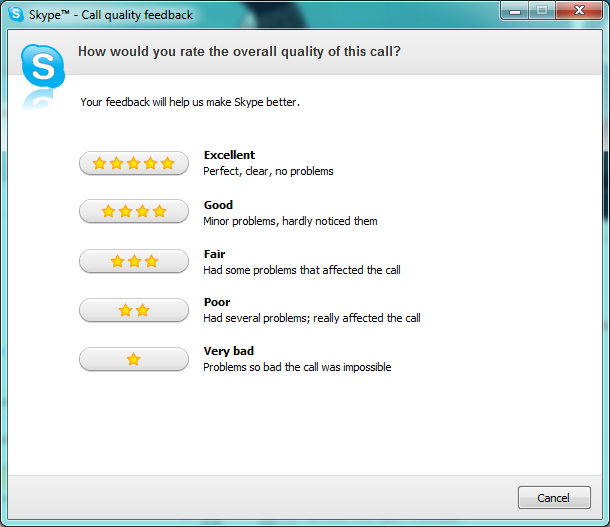
\includegraphics[trim=10px 100px 130px 25px, clip=true,scale=0.75]{figures/introduction/figures/skype.png}}
  \caption{Skype call quality rating (screenshot)}
  \label{fig:intro:fuzzy-skype}
\end{figure}

As a real-world example of fuzzy errors, consider the case of a voice
over IP service such as Skype\footnote{\url{https://www.skype.com}}.
%
After the call is made, the user can be asked to rate the quality of
the call in terms of stars: $1$ star $\rightarrow$ very bad, $5$ stars
$\rightarrow$ excellent (\Cref{fig:intro:fuzzy-skype}).
%
Intuitively, we can see that a binary error logic abstracts available
information from the diagnostic engine as a two-valued logic cannot
encode the same information as five-valued logic.

The challenge of solving this limitation is thereby twofold.
%
First, it is necessary to define an appropriate method for both
detecting and abstracting non-functional errors and the associated
error symptoms.
%
Second, it is necessary to integrate the additional knowledge in the
diagnostic process.

\researchquestion{How to encode fuzzy error
  symptoms?\label{rq:fuzzy-error-encoding}}
%
\researchquestion{How to improve \ac{SFL} to make use of the fuzzy
  error information?\label{rq:SFL-fuzzy-error-generalization}}
\subsubsection{System State}
\label{sec:intro:research-goals:system-state}

%% Problem 1: limited abstraction
A limitation of the \ac{SFL} approach presented in
\Cref{sec:intro:candidate-ranking} is related to the high level of
abstraction enforced by the usage of hit spectra as it does not
provide any information about the state of the system during each
component's execution.
%
Additionally, it abstracts the number of times each component was used
and, consequently, the sequence in which they were used in each
transaction.
%
As a consequence, hit spectrum approaches are unable to distinguishing
pairs of components for which the activity is equal.

%% Problem 2: constant gj
Furthermore, the discussed \ac{SFL} approach estimates $g_j$ as being
constant with respect to a set of observations.
%
Consider that the effective (normally unknown) goodness for component
(\eg, a hard drive) was directly related to its lifetime and took
the shape of a sigmoid, gradually decreasing over time.
%
Due to the fact that, for a hard drive, the slope of the goodness
curve is small and the time is monotonic, $g_j$ can, most of the
times, be successfully approximated by a constant with small errors.
%
However, if the observations spanned over a long period or the slope
of the goodness curve was larger (\eg, for a floppy disk), a constant
goodness function would fail to accurately model the actual goodness,
entailing large average errors.
%
Given the multiplicative nature of the goodness value usage, even
small errors can have a serious impact in the diagnosis report
ranking.

%% Problem 3: incapacity to specialize
Finally, hit spectrum approaches are not able to incorporate existent
knowledge about the system in the diagnostic process.
%
As the state of the system is completely abstracted in the hit
spectrum, it would be impossible to distinguish, for instance, a new
hard drive from an old hard drive.
%
As a consequence, even if the actual goodness curve was available for
all components in the system, the algorithm would not be able to use
it.

\researchquestion{How to enable \ac{SFL} to adapt to different systems
  based on previous diagnostic experience?\label{rq:feedback}}
%
\researchquestion{How to incorporate information about the system's
  state in \ac{SFL}?\label{rq:system-state}}


\section{Origin of Chapters}
\label{sec:intro:origin-of-chapters}
\begin{description}
\item [\Cref{sec:mhs2o,sec:mhs2p}] are
  based on the work from \citep{Cardoso14a}, which was published in
  the proceedings of \textit{the 25th International Workshop on
    Principles of
    Diagnosis}\footnote{\url{http://dx-2014.ist.tugraz.at/}} (best
  paper award). An early version of the paper was also published in
  the proceedings of both the \textit{16th Portuguese Conference on
    Artificial Intelligence
    (EPIA)}\footnote{\url{http://www.epia2013.uac.pt/}}
  \citep{Cardoso13b} and the \textit{International Conference on
    Multi-core Software Engineering, Performance, and Tools
    (MUSEPAT)}\footnote{\url{http://eventos.fct.unl.pt/musepat2013/}}
  \citep{Cardoso13c}.

\item [\Cref{sec:fuzzinel}] is based on the work from
  \citep{Cardoso14b}, which was published in the proceedings of
  \textit{the 25th International Workshop on Principles of Diagnosis}
  (best paper award nominee).

\item [\Cref{sec:nfge}] is based on the work from \citep{Cardoso13a},
  which was published in the proceedings of the \textit{27th AAAI
    Conference on Artificial Intelligence
    (AAAI)}\footnote{\url{http://www.aaai.org/Conferences/AAAI/aaai13.php}}.
\end{description}

\section{Thesis Outline}
\label{sec:intro:outline}
In \Cref{fig:intro:outline} we present the thesis outline.
%
We suggest a pre-order traversal of the tree, from top to bottom.
%




\begin{figure}[!ht]
  \begin{tikzpicture}
    [scale=1.9,
    mindmap,
    every node/.style={align=center,
      concept,
      execute at begin node=\hskip0pt,
      text=black,
      fill=white,
      line width=0.5em},
    grow cyclic,
    level 1/.append style={clockwise from=67.5,level distance=3cm,text width=3.25cm,sibling angle=135},
    level 2/.append style={clockwise from=40,level distance=2.5cm,sibling angle=80,text width=3cm,font=\small},
    level 3/.append style={clockwise from=0,level distance=2.25cm,sibling angle=45,text width=2.5cm,font=\small},]
    % \hyphenpenalty10000

    \node [text width=4cm,concept color=green!20!red] {SFL \\[0.5em] Section \ref{sec:intro:SFL}} % root
    [ concept color=green!20!red]
    child [concept color=red!90!yellow] { node {Candidate\\Generation \\[0.5em] Section \ref{sec:intro:candidate-generation}}
      child [concept color=red!80!yellow] { node  { Research\\Goals \\[0.5em] Section \ref{sec:intro:research-goals:algorithmic-efficiency}}
        child { node {\mhsII{} \\[0.5em] Chapter \ref{sec:mhs2o}} }
      }
      child [concept color=red!70!yellow] { node {Research\\Goals \\[0.5em] Section \ref{sec:intro:research-goals:horizontal-scalability}}
        child { node  {\mhsII{} \\[0.5em] Chapter \ref{sec:mhs2p}} }
      }
    }
    child [concept color=red!60!yellow] { node {Candidate\\Ranking \\[0.5em] Section \ref{sec:intro:candidate-ranking}}
      child [concept color=red!50!yellow] { node {Research\\Goals \\[0.5em] Section \ref{sec:intro:research-goals:fuzzy-errors}}
        child { node {\fuzzinel{} \\[0.5em] Chapter \ref{sec:fuzzinel}} }
      }
      child [concept color=red!40!yellow] { node {Research\\Goals \\[0.5em] Section \ref{sec:intro:research-goals:system-state}}
        child { node {\NFGE{} \\[0.5em] Chapter \ref{sec:nfge}} }
      }
    };
  \end{tikzpicture}
  \caption{Thesis outline\label{fig:intro:outline}}
\end{figure}

\renewcommand{\BrainFuckChapter}{y}
\renewcommand{\LifeChapter}{y}
\chapter{Background}
\label{chap:background}
\chaptertoc{}

\begin{chapterabstract}
  This chapter introduces the physics behind \ac{dMRI}, some techniques used for the simulation of \ac{dMRI} as well as some background on axonal growth mechanisms.
  Firstly, general MR physics is introduced building up from a single proton to the generation of the spin echo signal.
  The second section discusses how the diffusion of water molecules impacts the MR signal, leading to the diffusion signal attenuation.
  The third section introduces some simulation approaches which can be used to generate synthetic \ac{dMRI} data.
  % The final section gives an overview of some of the mechanisms which drive axonal growth in nature and which for the inspiration for the synthetic growth algorithm presented in further chapters.
  The final section gives a brief overview of the kinds of \ac{dMRI} models typically used in the brain with a focus on spherical deconvolution techniques which will be used later in the thesis.
\end{chapterabstract}

\section{MR Physics}
\label{sec:bg_mri_physics}
All forms of \emph{in vivo} use of magnetic resonance have their origins in the 1940s when Purcell, Torrey and Pound independently and almost simultaneously with Bloch, Hansen and Packard detected radio frequency signals from nuclei in ordinary matter\cite{Levitt2008, Barker2009,Bloch1946,Purcell1946}.
This discovery gave birth to the field of \ac{NMR} which has become widespread, with applications in a number of areas including chemistry, biology, materials science and medical imaging\cite{Barker2009, Salibi1998}.

Within the medical imaging context, \ac{NMR} typically finds two uses, \acf{MRI} and \ac{MRS}\footnote{The `N' from NMR is dropped in the medical imaging context to avoid confusion with nuclear medicine and general squeamishness around the word nuclear}.
Both of these uses are closely related: \ac{MRI} is typically concerned with building images of internal structures in the body, whilst \ac{MRS} is concerned with identifying the chemical composition of tissues in the body.

The theory behind \ac{NMR} concerns the interaction between nuclei and magnetic fields. This section briefly introduces the \ac{NMR} physics relevant to \ac{dMRI}.

\subsection{Nuclear Magnetism}
\label{sec:bg_nuclearmagnetism}

The most important property of a nucleus for the application of \ac{NMR} is nuclear spin. 
Spin is a property inherent to all subatomic particles and whilst it is a purely quantum effect, it can be thought of loosely as the particle spinning around its axis - much like a tiny planet \cite{Levitt2008}.
A planet spinning about its axis will have an angular momentum associated with that rotation and similarly the spin of a particle behaves like an angular momentum.
Unlike the angular momentum of a rotating planet, however, the spin is an intrinsic property of the particle itself and not a result of its motion\cite{Levitt2008}.

\begin{comment}
One of the postulates of quantum mechanics is that angular momentum is quantised \cite{DeGraaf2007}. This means that the spin angular momentum, $S$, of a particle in its rest state can only take values of
\begin{equation}
S = \hbar \sqrt{(I(I+1))} \,,
\label{eq:angmom_quant}
\end{equation} 
where $I$ is the spin angular momentum quantum number which can only take integer or half-integer values and $\hbar$ is the reduced Planck constant \cite{DeGraaf2007}.
A second quantum number is used to describe the direction of angular momentum relative to a given direction, usually referred to as $z$. 
Again, this quantum number is quantised, with the angular momentum in the $z$ direction, $S_z$, given by 
\begin{equation}
S_z = \hbar m_z \,.
\label{eq:angmom_z}
\end{equation} 
The $m_z$ quantum number can have $2I + 1$ values in the range \cite{DeGraaf2007}
\begin{equation}
m_z = -I,\, -I + 1,\,\dots,\, I-1,\, I\,.
\label{eq:m_z}
\end{equation}

Protons, neutrons and electrons - the particles making up all everyday matter - all have a spin quantum number of $I = \sfrac{1}{2}$ meaning that $m_z$ can have two possible values $m_z = \pm \sfrac{1}{2}$.


% \todo{IS THIS BIT NECESSARY? JUST FOCUS ON PROTONS?}
% Nuclei are made up of protons and neutrons, so the spin of a nucleus will be given by the combination of the spins of the protons and neutrons in the nucleus.
% In general in quantum mechanics, the combination of two angular momenta will result in a third angular momentum, which can take a range of values according to 
% \begin{equation}
% I_{12} = |I_1 - I_2|, |I_1-I_2| + 1, \dots, |I_1 + I_2| - 1, |I_1 + I_2|\,. 
% \end{equation}
 
% The precise way in which the spins combine in any given nucleus is a complicated quantum mechanical problem but there are some rules which describe the possible nuclear spin quantum numbers. 
% A nucleus with an odd mass number will have a half-integer spin, a nucleus with even mass number and even atomic number will have zero spin and a nucleus with an even mass number and odd atomic number will have integer spin \cite{DeGraaf2007}.

This project is focused on \ac{NMR} of \ce{^1H} nuclei in water molecules, which simply consist of a single proton and so have $I = \sfrac{1}{2}$. 
\ac{NMR} is, however, feasible on any nucleus with non-zero spin with some of the most biologically relevant nuclei for in-vivo MRS being \ce{^{13}C}, \ce{^{31}P} and \ce{^{23}Na} \cite{DeGraaf2007}.
\end{comment}


\ac{MRI} typically relies on \ac{NMR} of \ce{^1H} nuclei in water molecules, which simply consist of a single proton.
A proton carries a positive electric charge.
Just as classically a rotating charge with angular momentum, $\mathbf{L}$, will produce a magnetic moment, $
\boldsymbol{\mu} = \gamma \mathbf{L}$, the intrinsic spin angular momentum, $\mathbf{S}$ of a proton will produce a magnetic moment 
\begin{equation}
\label{eq:magnmom}
\boldsymbol{\mu} = \gamma \mathbf{S} \,,
\end{equation}
where $\gamma$ is the gyromagnetic ratio \cite{Levitt2008}.
For a proton, $\gamma = 2.675 \times 10^8$ rad s$^{-1}$ T$^{-1}$.

The fact that a proton has an intrinsic magnetic moment means that it will interact with magnetic fields and it is understanding this interaction that underpins \ac{NMR} theory.


\subsection{Magnetic Resonance}
\label{sec:bg_resonance}
Classically, a magnetic moment, $\boldsymbol{\mu}$, placed in an external magnetic field, $\mathbf{B}_0$, will feel a torque, $\boldsymbol{\tau}$, given by \cite{Haacke1999} 
\begin{equation}
\label{eq:torque}
\boldsymbol{\tau} = \boldsymbol{\mu} \times \mathbf{B}_0 \,.
\end{equation}
At the same time, classical mechanics gives a relationship between the change in angular momentum and the torque as \cite{Haacke1999} 
\begin{equation}
\label{eq:dLdt}
\frac{d\mathbf{L}}{dt} = \boldsymbol{\tau}\,. 
\end{equation}
For a proton in its rest state, the only angular momentum is the intrinsic spin angular momentum, $\mathbf{S}$, so combining \Cref{eq:torque,eq:dLdt} gives the equation of motion for a spin in an external magnetic field
\begin{equation}
\frac{d\mathbf{S}}{dt} = \boldsymbol{\mu} \times \mathbf{B}_0 \,.
\end{equation}
Since $\mathbf{S}$ is equivalent to $\boldsymbol{\mu}/\gamma$ (\Cref{eq:magnmom}), this becomes
\begin{equation}
\frac{d\boldsymbol{\mu}}{dt} = \gamma\boldsymbol{\mu} \times \mathbf{B}_0\,.
\label{eq:dmudt}
\end{equation}

This equation of motion can be solved in a few ways for the case of constant external magnetic field, with the result being that the magnetic moment precesses about the magnetic field with a frequency, $\omega_0$, given by\cite{Levitt2008}
\begin{equation}
\label{eq:LarmorFreq}
\omega_0 = \gamma B_0\,,
\end{equation}
with $B_0$ being the external field strength. 
This precessional motional is illustrated in \Cref{fig:precession}.
The frequency $\omega_0$ is known as the Larmor frequency and lies in the \ac{RF} range for typical field strengths found in MRI machines (1.5 - 7 T).

\begin{figure}
	\centering
	\begin{subfigure}{0.3\textwidth}
		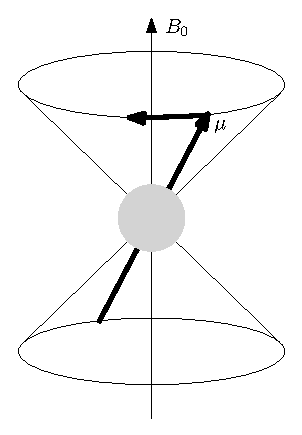
\includegraphics[width = \textwidth]{figures/background/precession.eps}
		\caption{}
		\label{fig:precession}
	\end{subfigure}
	\hspace{2cm}
	\begin{subfigure}{0.3\textwidth}
		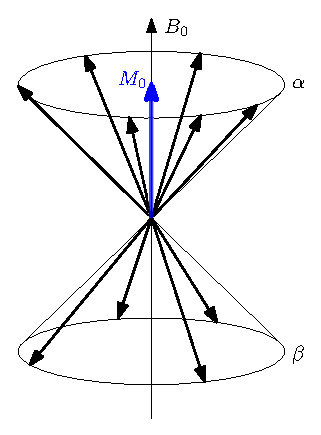
\includegraphics[width = \textwidth]{figures/background/manyspins.eps}
		\caption{}
		\label{fig:manyspins}
	\end{subfigure}
	
	\caption[Illustration of the precessional motion of a single spin and production of magnetisation by many spins]{a) Illustration of the precessional motion of a single spin with magnetic moment $\mu$ in the presence of an external magnetic field $B_0$. b) Many individual spins in an external magnetic field precess around the external field with random phase producing a net magnetisation in the direction of the $B_0$ field.}
	\label{fig:precession-spins}
	
\end{figure}


In practice, it is not possible to observe the magnetic moment of a single spin. 
The quantity observed is rather the sum of the magnetic moments from many spins together, this is known as the net magnetisation. 
%In order to fully describe the system, a quantum mechanical treatment using density operators is necessary \cite{Levitt2008}, however a classical treatment is sufficient to understand the basic principles.

\begin{comment}
As mentioned in \Cref{sec:bg_nuclearmagnetism}, protons can have two $S_z$ states with $m_z = \pm \sfrac{1}{2}$. 
These states can be thought of as the magnetic moment either being aligned parallel or anti-parallel to the external magnetic field, known as spin-up and spin-down respectively.

\begin{figure}
	\centering
	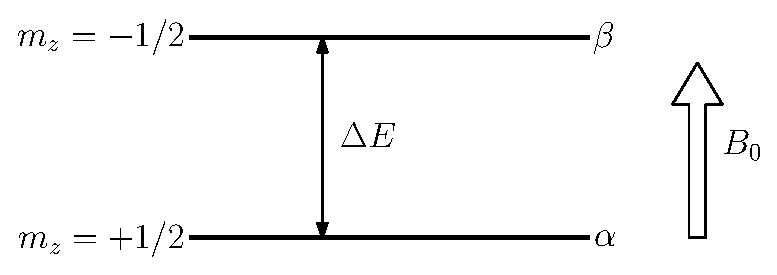
\includegraphics[width=0.6\textwidth]{figures/background/energy_levels.eps}
	\caption{Energy levels of a spin-1/2 particle. The spin-up state ($\alpha$) has the lowest energy and the spin down state ($\beta$) has the highest. The energy difference between the levels is $\Delta E$.}
	\label{fig:energylevels}
\end{figure}

The energy difference between these two states is given by a quantum mechanical effect called the Zeeman effect \cite{Levitt2008}, which gives the difference as  
\begin{equation}
	\Delta E = \gamma \hbar B_0\,.
\end{equation} 

\Cref{fig:energylevels} illustrates this splitting of the energy levels showing that the spin-up state, $\alpha$, is the lower of the two energy states. 
When there are many protons all experiencing the same magnetic field, the proportion of the number of protons in the spin-up, $n_\alpha$, state versus spin-down, $n_\beta$, is given by the Boltzmann distribution\cite{DeGraaf2007}
\begin{equation}
\frac{n_\alpha}{n_\beta} = \exp\left(\frac{\Delta E}{k_BT}\right)\,,
\end{equation}  
where $k_B$ is the Boltzmann constant and $T$ is the temperature. This means that at a non-zero temperature and with positive $\gamma$, there are slightly more protons aligned with the magnetic field than against it.  
\end{comment}


In a sample, slightly more protons will align with the $\mathbf{B}_0$ field than against it, meaning that the net magnetisation will be parallel to $\mathbf{B}_0$. 
\Cref{fig:manyspins} shows a pictorial representation of the system of many spins producing a net magnetisation, $\mathbf{M}_0$ aligned with $\mathbf{B}_0$.

Each of the spins will still be precessing about the magnetic field at the Larmor frequency but since they are out of phase with one another, all transverse components of the magnetisation cancel out when they combine and all that is left is a static longitudinal component. 


In order to make measurements, the net longitudinal magnetisation needs to be `flipped' into the transverse plane where it can be detected. 
This is achieved by applying a second magnetic field, $\mathbf{B}_1$, oscillating in the transverse plane. 
In much the same way as with $\mathbf{B}_0$, the magnetisation feels a torque from $\mathbf{B}_1$ and begins to rotate about $\mathbf{B}_1$, away from the longitudinal axis.
The two external fields act simultaneously on $\mathbf{M}_0$ so the magnetisation will tip away from the $z$ axis whilst still precessing about $z$ with a frequency $\omega_0$.
This kind of motion is known as nutation and is illustrated in \Cref{fig:nutation}.

\begin{figure}
	\centering
	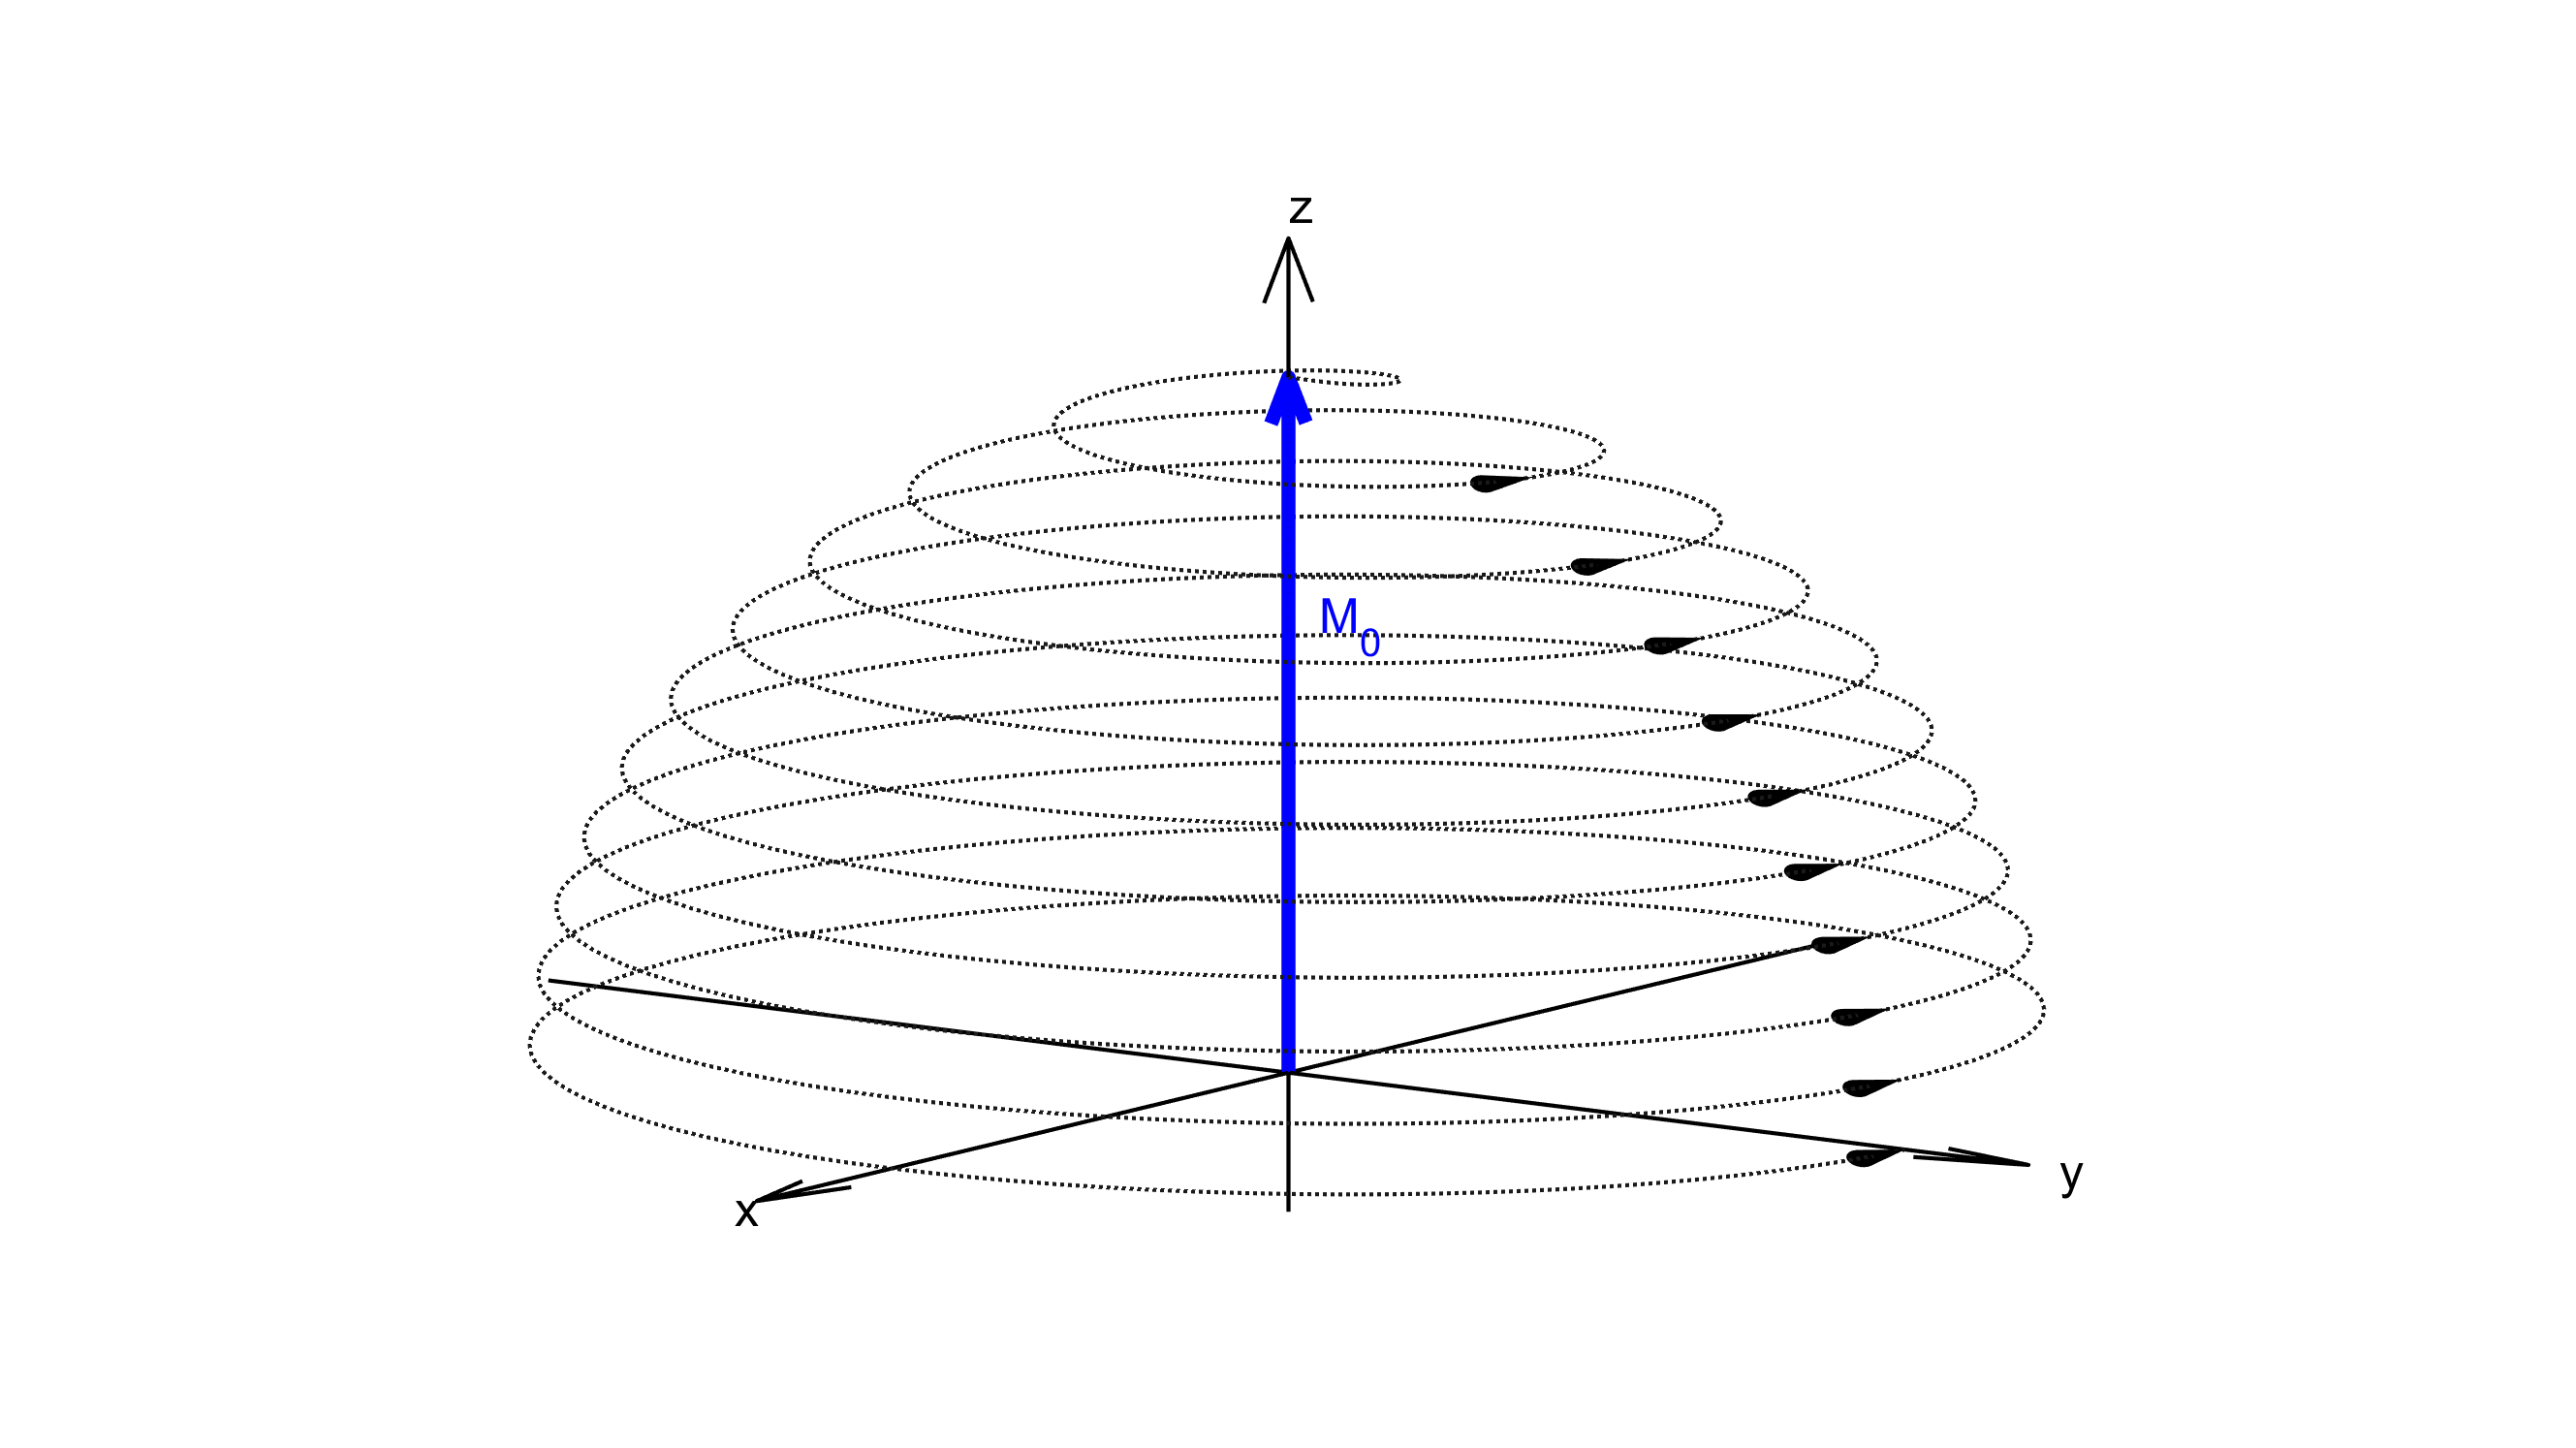
\includegraphics[width=\textwidth]{figures/background/nutation.eps}
	\caption[Nutation motion of an on-resonance spin the presence of an \acs{RF} field.]{Nutation motion of an on-resonance spin in the presence of an \ac{RF} field. Precession about the $B_0$ and $B_1$ fields create the spiralling motion in the laboratory frame.}
	\label{fig:nutation}
\end{figure}



\subsection{The Bloch Equations}
\label{sec:bg_bloch}
The interaction between the magnetisation and magnetic fields is described by the Bloch equations - an empirical set of equations describing the evolution of magnetisation introduced by Felix Bloch in 1946\cite{Bloch1946}.

The magnetisation arises from a sum of independent magnetic moments, meaning that we can represent the magnetisation as 
\begin{equation}
	\mathbf{M} = \sum_i \boldsymbol{\mu}_i \,,
        \label{eq:net_magnetisation}
\end{equation}
with $i$ indicating a sum over all the spins in the sample.
This definition for $\mathbf{M}$ can be combined with the equation of motion for a single spin, \Cref{eq:dmudt}, to give \cite{Haacke1999}
\begin{equation}
	\frac{d\mathbf{M}}{dt} = \gamma \mathbf{M} \times \mathbf{B}\,.
	\label{eq:dMdt}
\end{equation}  

In the presence of the main external field, $\mathbf{B}_0$, the magnetisation will be static and aligned along the $z$ axis. The $x$ and $y$ components of the magnetisation will have random orientations and precess about $\mathbf{B}_0$ at the Larmor frequency with a mean amplitude of zero. This will give the components of \Cref{eq:dMdt} as\cite{DeGraaf2007}
\begin{align}
	\frac{d\mathbf{M}_x(t)}{dt} &= \gamma\mathbf{M}_y\mathbf{B}_0\,,\\
	\frac{d\mathbf{M}_y(t)}{dt} &= -\gamma\mathbf{M}_x\mathbf{B}_0\,,\\	\frac{d\mathbf{M}_z(t)}{dt} &= 0 \,.
\end{align}

To understand the interaction of the magnetisation with the $\mathbf{B}_1$ field, the oscillation of the field in the transverse plane needs to be described. 
%The $\mathbf{B}_1$ field is oscillating in the transverse plane, say, along the $x$-axis. 
%The linearly oscillating field in $x$ can be thought of as two components rotating about the $z$-axis, one with a frequency $\omega$ and one with a frequency $-\omega$. 
%The sum of these two components will result in a field that is linearly oscillating along $x$ with a frequency $\omega$. \todo{Change/Mention that circularly polarised fields are used}
%
%Supposing that this frequency is on the same order as the Larmor frequency, one of the components (for a spin with positive $\gamma$ this will be the $+\omega$ component) will differ from the Larmor frequency by about $2\omega$. 
%This means that the effect of this component on the magnetisation can be neglected and the exciting magnetic field will have the form\cite{DeGraaf2007}
Usually, the $\mathbf{B}_1$ field is circularly polarised to oscillate in the transverse plane so that the field can be described as
\begin{equation}
	\mathbf{B}_1(t) = B_1\cos(\omega t) \mathbf{\hat{x}} - B_1\sin(\omega t) \mathbf{\hat{y}}\,,
	\label{eq:circB1}
\end{equation}
where $\mathbf{\hat{x}}$ and $\mathbf{\hat{y}}$ are unit vectors in the $x$ and $y$ directions respectively. 


The combined effect of the $\mathbf{B}_0$ and $\mathbf{B}_1$ fields can be seen from \Cref{eq:dMdt} to get \cite{DeGraaf2007}
\begin{align}
	\frac{d\mathbf{M}_x(t)}{dt} &= \gamma \left(\mathbf{M}_y(t)\mathbf{B}_0 - \mathbf{M}_z(t)\mathbf{B}_1\sin(\omega t)\right)\,,\label{eq:bloch_norelx}\\
	\frac{d\mathbf{M}_y(t)}{dt} &= \gamma \left(\mathbf{M}_z(t)\mathbf{B}_1\cos(\omega t) - \mathbf{M}_x(t)\mathbf{B}_0\right)\,,\label{eq:bloch_norely}\\
	\frac{d\mathbf{M}_z(t)}{dt} &= \gamma \left(\mathbf{M}_x(t)\mathbf{B}_1\sin(\omega t) - \mathbf{M}_y(t)\mathbf{B}_1\cos(\omega t) \right)\,.\label{eq:bloch_norelz}
\end{align}

These are the equations of motion of the magnetisation in the laboratory frame under the influence of the $\mathbf{B}_0$ and $\mathbf{B}_1$ and describe the kind of motion seen in \Cref{fig:nutation}. 

\subsubsection{Relaxation}
In order to get to the full Bloch Equations the concept of relaxation must be introduced. 
Relaxation is a term used to describe the way in which a spin system will return to equilibrium after being perturbed. The components of $\mathbf{M}$ that are parallel to the $\mathrm{B_0}$ magnetic field relax differently to those perpendicular to the magnetic field leading to two relaxation terms being introduced into \Cref{eq:bloch_norelx,eq:bloch_norely,eq:bloch_norelz}. 

The relaxation processes are exponential and described by two time constants, $\mathrm{T}_1$ and $\mathrm{T}_2$. $\mathrm{T}_1$ is the longitudinal relaxation time and describes the rate at which longitudinal magnetisation regrows after a perturbation. 
$\mathrm{T}_2$ is the transverse relaxation time and describes the rate at which transverse magnetisation decays after a perturbation. 
$\mathrm{T}_2$ is always shorter than $\mathrm{T}_1$ since all the effects which contribute to $\mathrm{T}_1$ also contribute to $\mathrm{T}_2$ relaxation, however $\mathrm{T}_2$ relaxation is also affected by the spins going out of phase with one another.
The relaxation process can be written as \cite{DeGraaf2007}
\begin{align}
	\frac{d\mathbf{M}_x(t)}{dt} &= -\frac{\mathbf{M}_x(t)}{\mathrm{T}_2}\,,\label{eq:bloch_rel1}\\
	\frac{d\mathbf{M}_y(t)}{dt} &= -\frac{\mathbf{M}_y(t)}{\mathrm{T}_2}\,,\label{eq:bloch_rel2}\\
	\frac{d\mathbf{M}_z(t)}{dt} &= -\frac{\mathbf{M}_z(t) - \mathbf{M}_0}{\mathrm{T}_1}\,.\label{eq:bloch_rel3}
\end{align}
		
Combining \Cref{eq:bloch_norelx,eq:bloch_norely,eq:bloch_norelz} and \Cref{eq:bloch_rel1,eq:bloch_rel2,eq:bloch_rel3} gives the full Bloch equations
\begin{align}
	\frac{d\mathbf{M}_x(t)}{dt} &= \gamma\left(\mathbf{M}_y(t)\mathbf{B}_0 - \mathbf{M}_z(t)\mathbf{B}_1\sin(\omega t)\right) - \frac{\mathbf{M}_x(t)}{\mathrm{T}_2}\,,\label{eq:bloch_labx}\\
	\frac{d\mathbf{M}_y(t)}{dt} &= \gamma\left(\mathbf{M}_z(t)\mathbf{B}_1\cos(\omega t) - \mathbf{M}_x(t)\mathbf{B}_0\right) - \frac{\mathbf{M}_y(t)}{\mathrm{T}_2}\,,\label{eq:bloch_laby}\\
	\frac{d\mathbf{M}_z(t)}{dt} &= \gamma \left(\mathbf{M}_x(t)\mathbf{B}_1\sin(\omega t) - \mathbf{M}_y(t)\mathbf{B}_1\cos(\omega t) \right) - \frac{\mathbf{M}_z(t) - \mathbf{M}_0}{\mathrm{T}_1}\,. \label{eq:bloch_labz}
\end{align}

$\mathrm{T}_2$ is used to refer to relaxation due to intrinsic spin-spin interactions which cause spins to accrue phase relative to one another and thus the magnitude of the net transverse magnetisation is reduced when taking the sum in \Cref{eq:net_magnetisation} .
Other effects can also contribute to the loss of transverse magnetisation, such as magnetic field inhomogeneities which can add to the $\mathrm{T}_2$ relaxation.
This is referred to as $\mathrm{T}_2^*$, with
\begin{equation}
  \frac{1}{\mathrm{T}_2^*} = \frac{1}{\mathrm{T}_2} + \frac{1}{\mathrm{T}_2'}\,,
  \label{eq:t2star}
\end{equation}
where $\mathrm{T}_2'$ is the relaxation time associated with these external sources and $\mathrm{T}_2$ is the intrinsic spin-spin relaxation time. The $\mathrm{T}_2'$ effect can be negated using special MR pulse sequences which will be covered in \Cref{sec:spin_echoes}, however the intrinsic $\mathrm{T}_2$ relaxation cannot be avoided.  


\subsubsection{The rotating frame}
To this point, everything has been described in a static Cartesian frame known as the laboratory frame. 
The lab frame is not the most convenient reference frame to analyse the \ac{NMR} experiment in, however.
Moving to a frame which is rotating about $\mathbf{B}_0$ (i.e.\ the $z$-axis) at a frequency $\omega$ matching the $\mathbf{B}_1$ field oscillation simplifies the maths of the system. 
The axes of this rotating frame will be referred to as $x', y'$ and $z'$. 

The components of the magnetisation in the rotating frame can be calculated from the lab frame components as \cite{DeGraaf2007}
\begin{align}
	\mathbf{M}_x' &= \mathbf{M}_x\cos(\omega t) - \mathbf{M}_y\sin(\omega t)\,,\\
	\mathbf{M}_y' &= \mathbf{M}_x\sin(\omega t) - \mathbf{M}_x\cos(\omega t)\,,\\
	\mathbf{M}_z' &= \mathbf{M}_z\,.
\end{align}

The rotating frame Bloch equations can be calculated by combining these rotating frame magnetisation components with the lab frame Bloch equations\cite{DeGraaf2007}
\begin{align}
	\frac{d\mathbf{M}_x'(t)}{dt} &= \Omega\mathbf{M}_y'(t) - \frac{\mathbf{M}_x'(t)}{\mathrm{T}_2}\,,\label{eq:blochx}\\
	\frac{d\mathbf{M}_y'(t)}{dt} &= -\Omega\mathbf{M}_x'(t) + \gamma\mathbf{B}_1\mathbf{M}_z'(t) - \frac{\mathbf{M}_y'(t)}{\mathrm{T}_2}\,,\label{eq:blochy}\\
	\frac{d\mathbf{M}_z'(t)}{dt} &= -\gamma\mathbf{B}_1\mathbf{M}_y'(t) - \frac{\mathbf{M}_z'(t) - \mathbf{M}_0}{\mathrm{T}_1}\,,\label{eq:blochz}
\end{align} 
where $\Omega = \omega_0 - \omega$ is the offset frequency between the $\mathbf{B}_1$ field frequency and the Larmor frequency. 

Since the frame is rotating with a frequency $\omega$, the $\mathbf{B}_1$ field appears static in the rotating frame. 
The precessional motion that is seen in the lab frame ($\omega_0 = \gamma\mathbf{B}_0$) is reduced to a frequency $\Omega$ in the rotating frame. 
When $\Omega = 0$, meaning that $\mathbf{B}_1$ oscillates at the Larmor frequency, the magnetisation simply precesses about the $\mathbf{B}_1$ field towards the transverse plane as illustrated in \Cref{fig:onres}. 

\begin{figure}
	\centering
	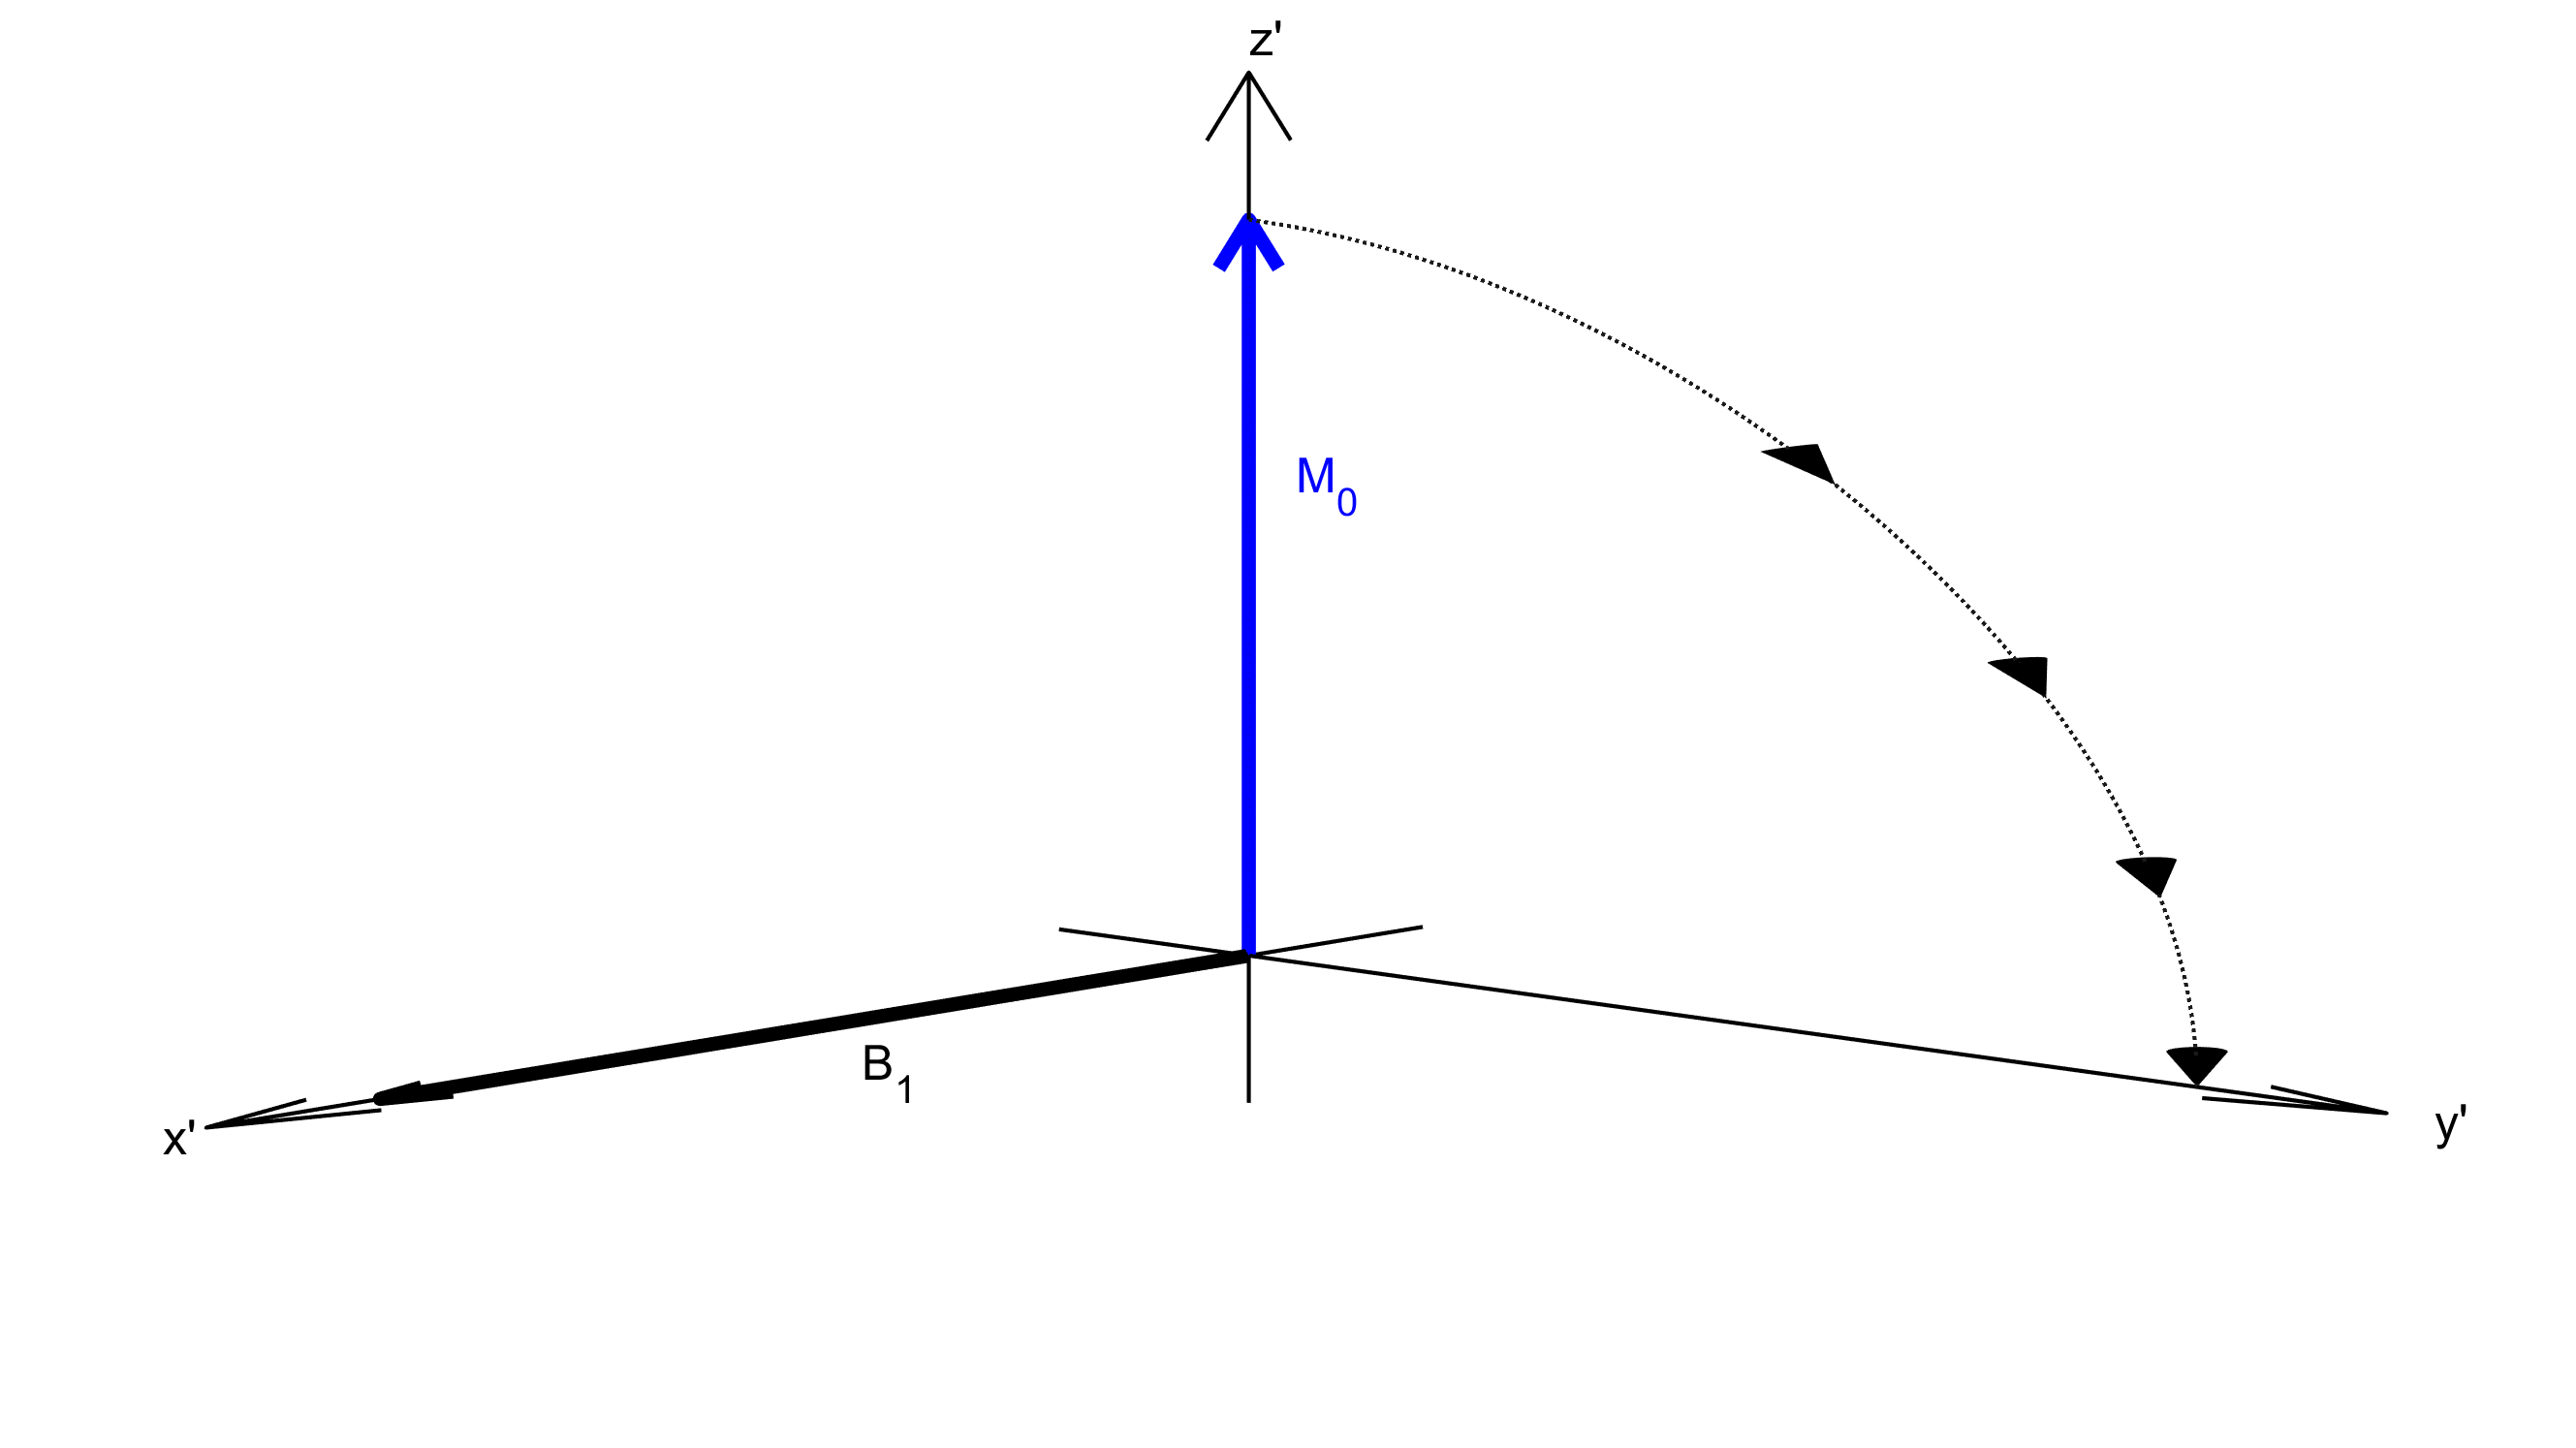
\includegraphics[width=\textwidth]{figures/background/nutation_onres.eps}
	\caption[Motion of a spin in the presence of a $B_1$ \acs{RF} field in the rotating frame]{Motion of a spin in the presence of a $B_1$ RF field in the rotating frame. This is identical to the nutation in \Cref{fig:nutation}, however viewing from the rotating frame simplifies the motion. }
	\label{fig:onres}
\end{figure}

This situation is known as resonance - the frequency of the \ac{RF} pulse matches the Larmor frequency, perfectly tipping the magnetisation away from the $z'$ axis and into the transverse plane. 

In the off-resonance case, an additional component of magnetic field with magnitude $\Omega/\gamma$ is produced in the $z$-direction.
This results in an effective magnetic field, $\mathbf{B}_e$, with a magnitude \cite{DeGraaf2007}
\begin{equation}
	B_e = |B_e| = \sqrt{B_1^2 + \left(\frac{\Omega}{\gamma}\right)^2}\,.
	\label{eq:Beff}
\end{equation}

%\todo[inline]{Do I need this off-resonance stuff? It's more geared towards introducing chemical shift for MRS. Perhaps just focus on signal generation?}
The effective field is illustrated in \Cref{fig:B_e} with the additional component of $\Omega/\gamma$ resulting in an effective field that is no longer aligned with $x'$.
\begin{figure}
	\centering
	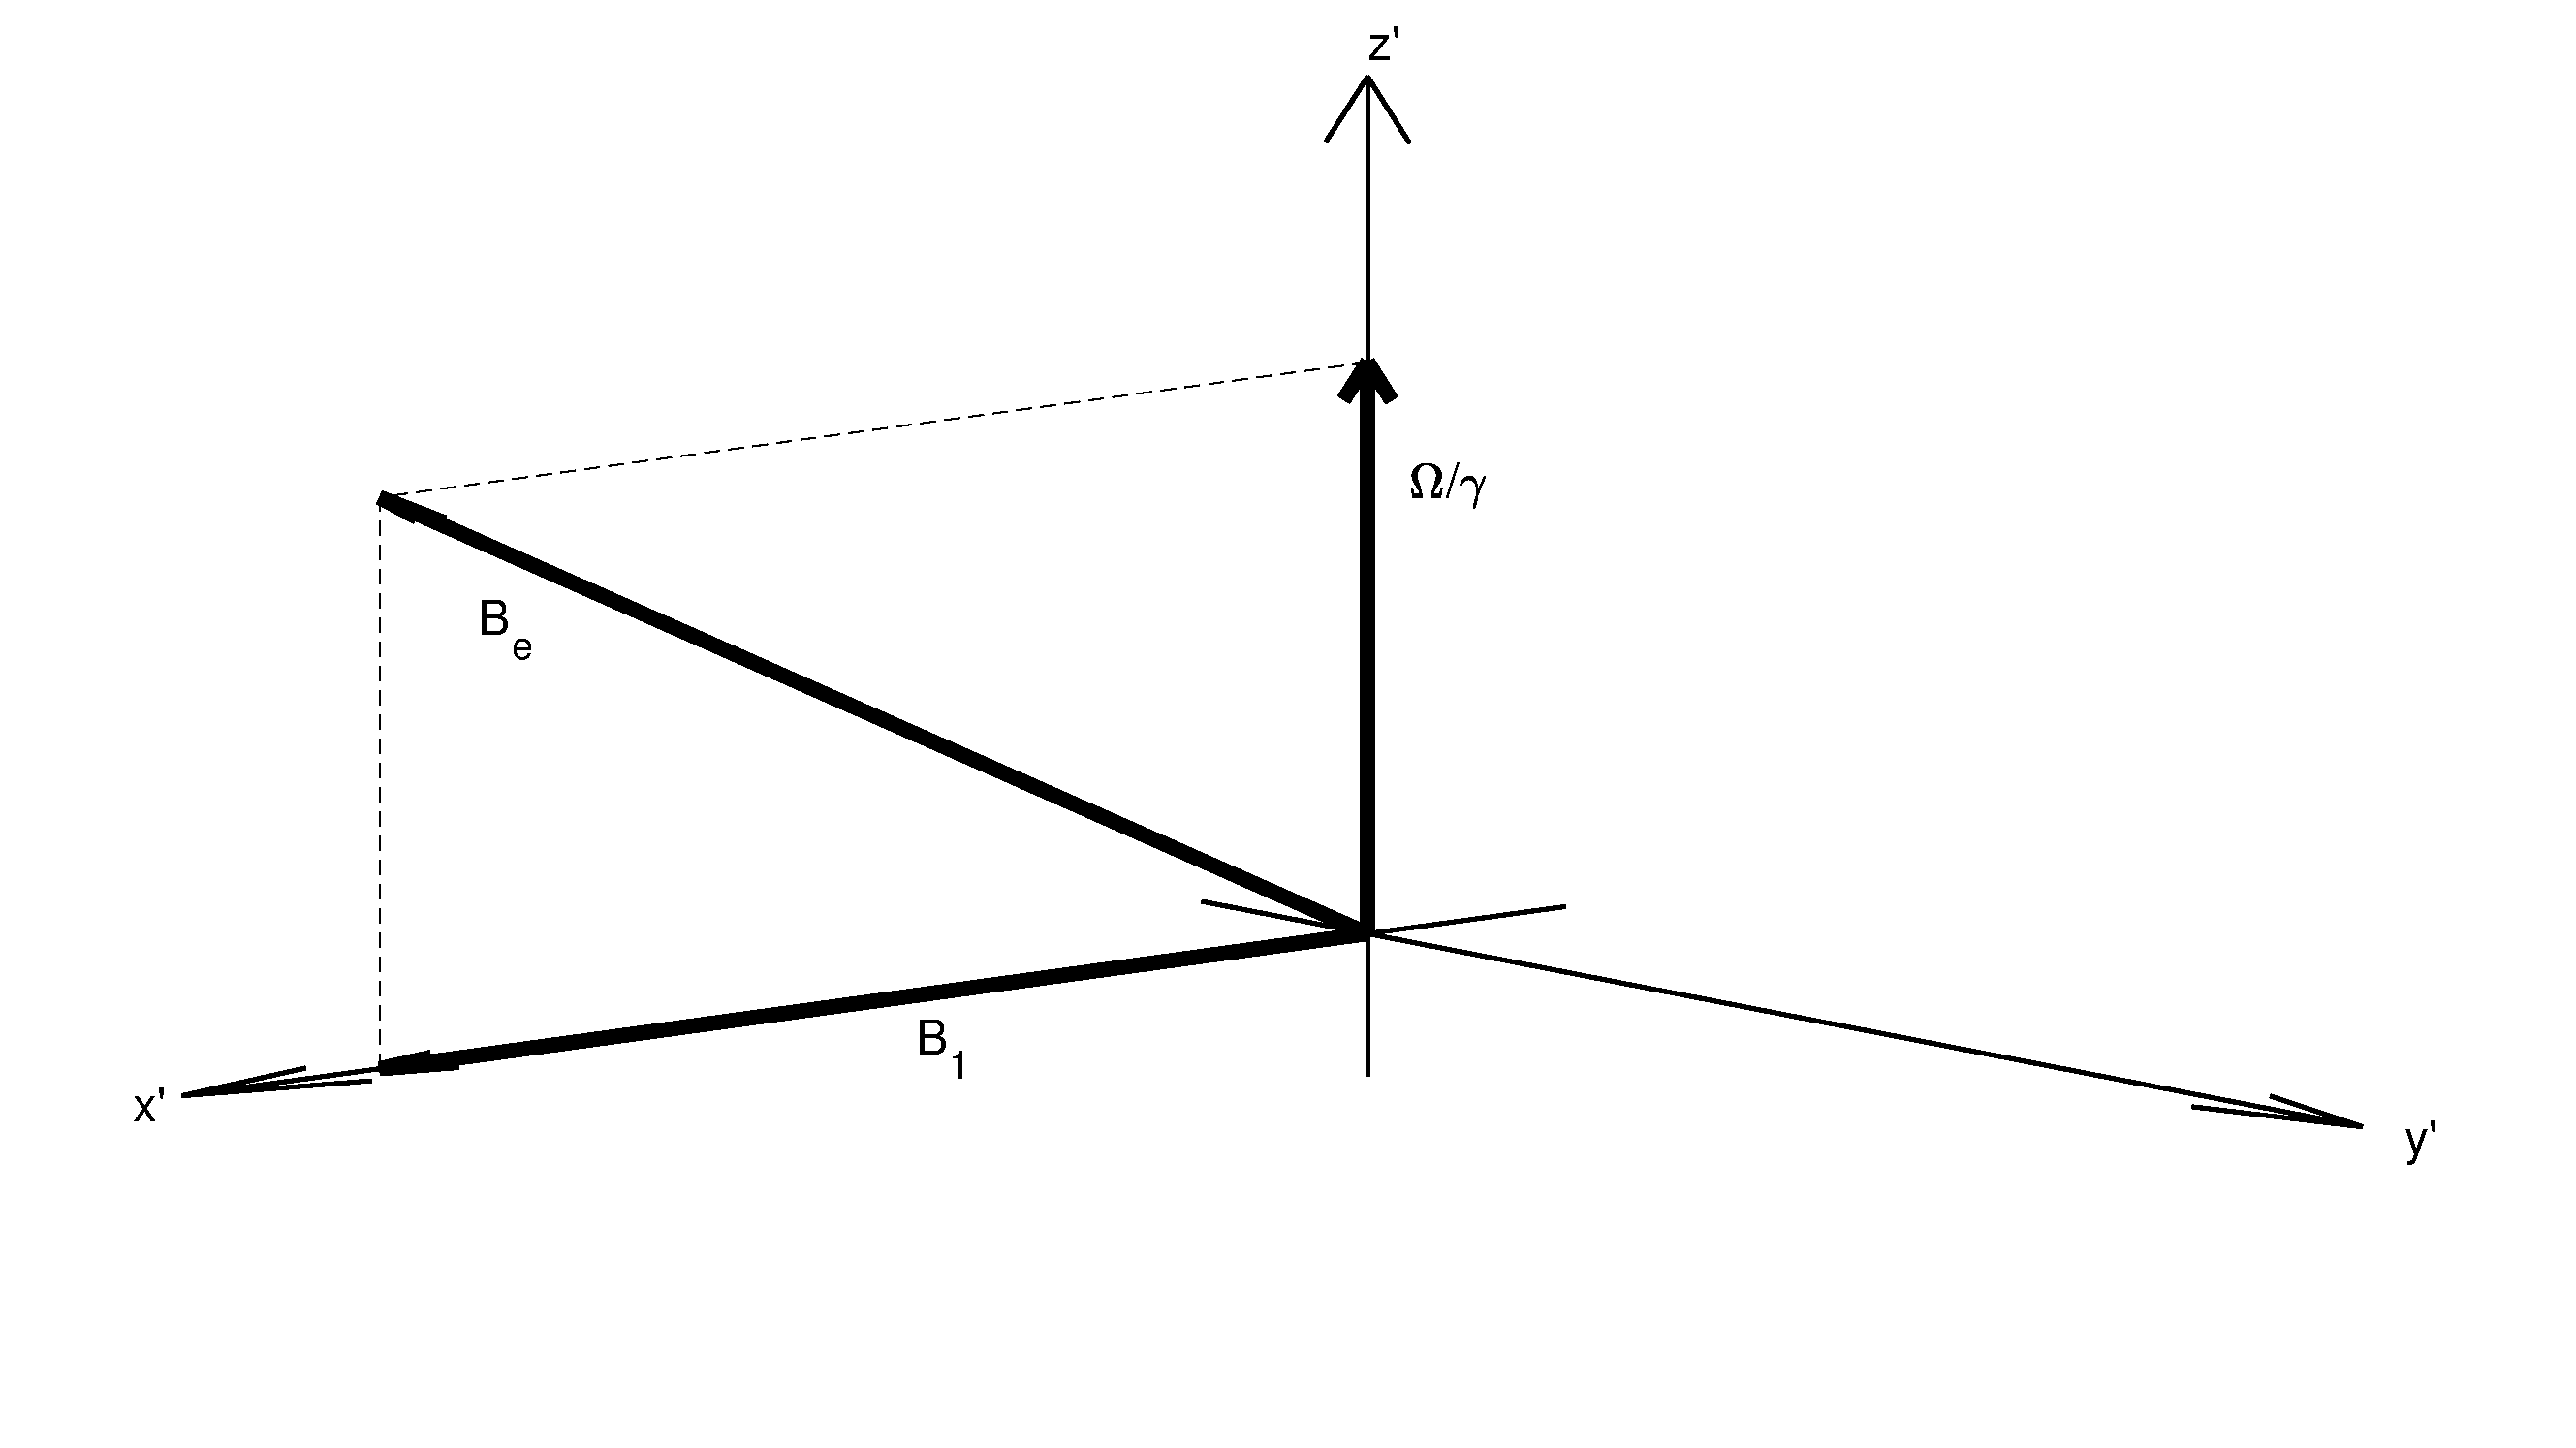
\includegraphics[width=\textwidth]{figures/background/B_e.eps}
	\caption[The effective field, $B_e$, produced due to an off-resonance frequency $\Omega$.] {The effective field, $B_e$, produced due to an off-resonance frequency $\Omega$. The off-resonance effects produce an additional component of magnetic field along the $z'$ axis.}
	\label{fig:B_e}	
\end{figure}
Off-resonance effects can produce unwanted results meaning the spin does not get flipped as much as expected under an \ac{RF} pulse which can result in signal losses. 
 

\subsection{Detecting the MR signal}
The detection and processing of \ac{NMR} signals is a deep topic which could be the subject of its own book, however some very basic details of how a signal is formed are useful to go on from here.
 
The reason for flipping the magnetisation into the transverse plane using $\mathbf{B}_1$ fields is to make the magnetisation detectable. 
Transverse magnetisation precesses about $\mathbf{B}_0$ at the Larmor frequency, sweeping its magnetic field around $\mathbf{B}_0$. 
A coil of wire placed near this precessing field will feel an electromotive force induced in it according to Faraday's Law of Induction\cite{Haacke1999}.

Following a pulse that flips the magnetisation from $\mathbf{M}_0$ aligned with $z$ through an angle $\beta$ towards $x'$, the $x'$-component of the magnetisation will be $M_0\sin\beta$ and (ignoring relaxation) will then precess at the offset frequency, $\Omega$, in the rotating frame. This will give the components of the magnetisation in the transverse plane over time as 
\begin{equation}
M_x = M_0\sin(\beta)\cos(\Omega t) \qquad M_y = M_0\sin(\beta)\sin(\Omega t)\,.\label{eq:MxMy}
\end{equation}

The signal induced into the receiver coils is proportional to $M_x$ and $M_y$ and so the signal will also have an oscillating form similar to \Cref{eq:MxMy}.
From the $\sin\beta$ term, it is clear that the maximum signal will arise when $\beta = 90$\degree, meaning all the magnetisation is flipped into the transverse plane. 
Additionally, in a realistic experiment, there will be $\mathrm{T_2^*}$ relaxation so including this, the general form of the signal following a 90\degree\ pulse will be\cite{DeGraaf2007} 
\begin{equation}
S_x = S_0\cos(\Omega t)\exp\left(-t/\mathrm{T}_2^*\right) \qquad S_y = S_0\sin(\Omega t)\exp\left(-t/\mathrm{T}_2^*\right)\,.
\end{equation}

Generally \ac{NMR} systems use something known as quadrature detection, meaning that both the $x'$ and $y'$ components of the magnetisation are measured simultaneously\cite{Levitt2008}, giving the signal as a function of time as 
\begin{align}
	S(t) &= S_x + iS_y\,,\nonumber\\
		 &= S_0\exp((i\Omega - 1/\mathrm{T}_2^*)t)\,.\label{eq:fid}
\end{align}  

\begin{figure}
  \centering
  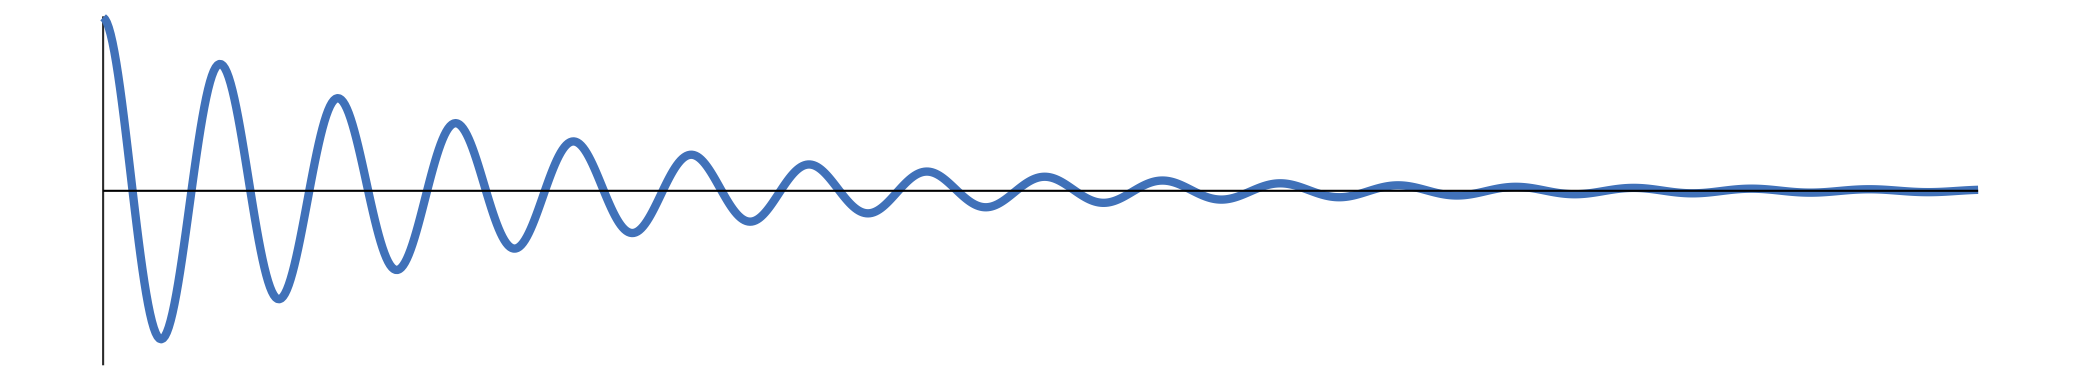
\includegraphics[width=\textwidth]{figures/background/FID_copy.png}
  \caption[The \acl{FID} described by \Cref{eq:fid}]{The \acl{FID} described by \Cref{eq:fid}. Here, just the real channel is plotted.}
  \label{fig:fid}
\end{figure}

This time-domain signal is known as a \ac{FID} and has a typical form shown in \Cref{fig:fid}. 
If we neglect off-resonance effects, then the \ac{FID} in the rotating frame will be a simple exponential decay.
\begin{equation}
  S(t) = S_0\exp(-t/\mathrm{T}_2^*)
  \label{eq:fid_rotframe}
\end{equation}

The \ac{FID} is not commonly used for \ac{dMRI} for a few reasons. Firstly, magnetic field gradients need to be introduced to make the signal sensitive to diffusion. Additionally, the $\mathbf{T}_2^*$ decay is often very rapid, so sequences known as spin echo sequences are used to remove the $\mathbf{T}_2'$ relaxation. 

\begin{comment}
The \ac{FID} holds all of the relevant information about the spin system needed for \ac{NMR}, however it is seldom used on its own since the information is difficult to interpret in this form.
\ac{NMR} spectroscopy uses a mathematical procedure known as the Fourier transform which is used as a transformation between the time and frequency domains. 
\begin{figure}
	\centering
	\begin{subfigure}{\textwidth}
		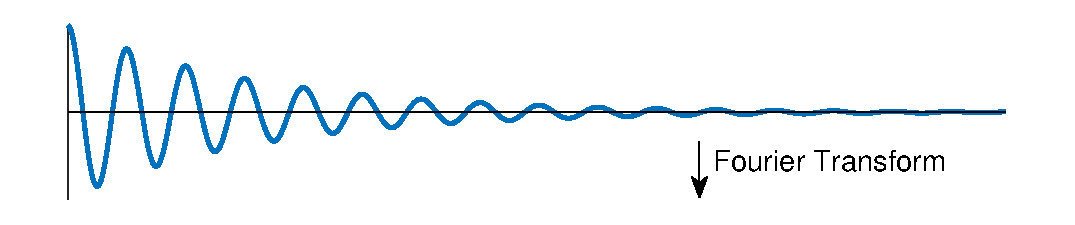
\includegraphics[width=\textwidth]{figures/background/FID.eps}
	\end{subfigure}

	\begin{subfigure}{\textwidth}
		
\includegraphics[width=\textwidth]{figures/background/fftFID.eps}
	\end{subfigure}
	\caption{An example of the Fourier transform. The time domain signal (top) is transformed into a frequency domain (bottom) by the Fourier transform. }
	\label{fig:fft}

      \end{figure}
      
Many books cover the Fourier transform in great detail \cite{Keeler2010, Haacke1999}, however for this report, it is sufficient to simply know its results.
The Fourier transform will take an \ac{FID} signal of the form in \Cref{eq:fid} and produce a frequency domain signal that has a mathematical form known as a Lorentzian, given by 
\begin{equation}
	S_0\exp((i\Omega - R_2)t) \quad\overset{\mathrm{FT}}{\rightarrow}\quad \frac{S_0R_2}{R_2^2 + (\omega - \Omega)^2} + i\frac{S_0(\omega - \Omega)}{R_2^2 + (\omega - \Omega)^2}\,,
\end{equation}    
where $\omega$ is the frequency domain of the spectrum. 
The real part of this term is known as the absorption mode and the imaginary part is known as the dispersion mode.
The absorption mode Lorentzian is shown in the bottom plot in \Cref{fig:fft}. 
Peaks like this form the basis of all spectra used in \ac{NMR} spectroscopy. 
\end{comment}



\subsection{Spin echoes}
\label{sec:spin_echoes}
\begin{figure}
	\centering
	\begin{subfigure}{0.9\textwidth}
		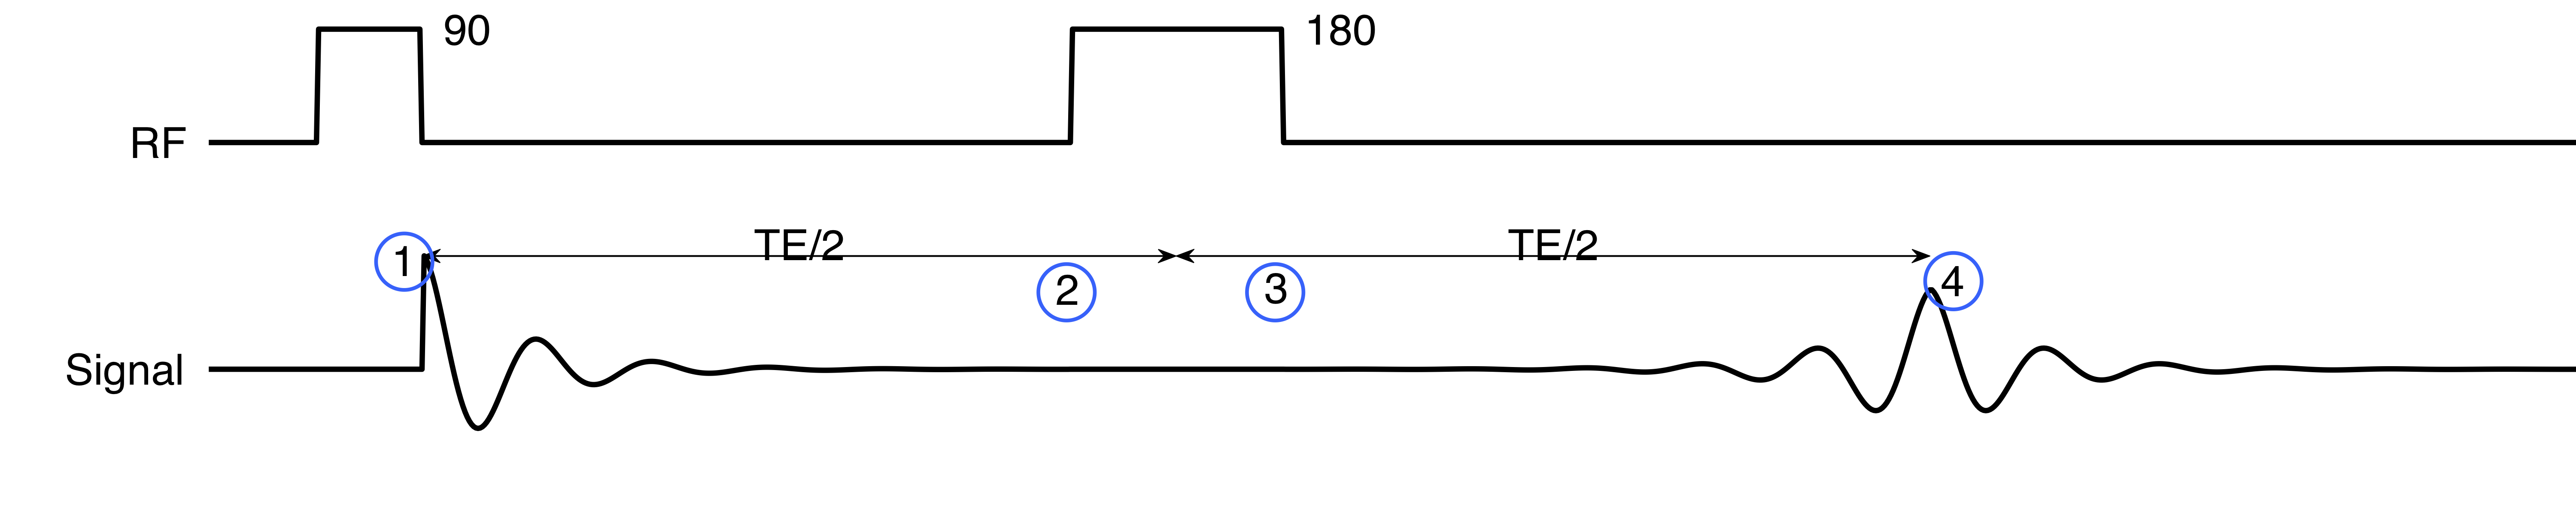
\includegraphics[width = \textwidth]{figures/background/spinecho.png}
		\caption{}
		\label{fig:spinechosequence}
	\end{subfigure}
	
	\begin{subfigure}{0.9\textwidth}
		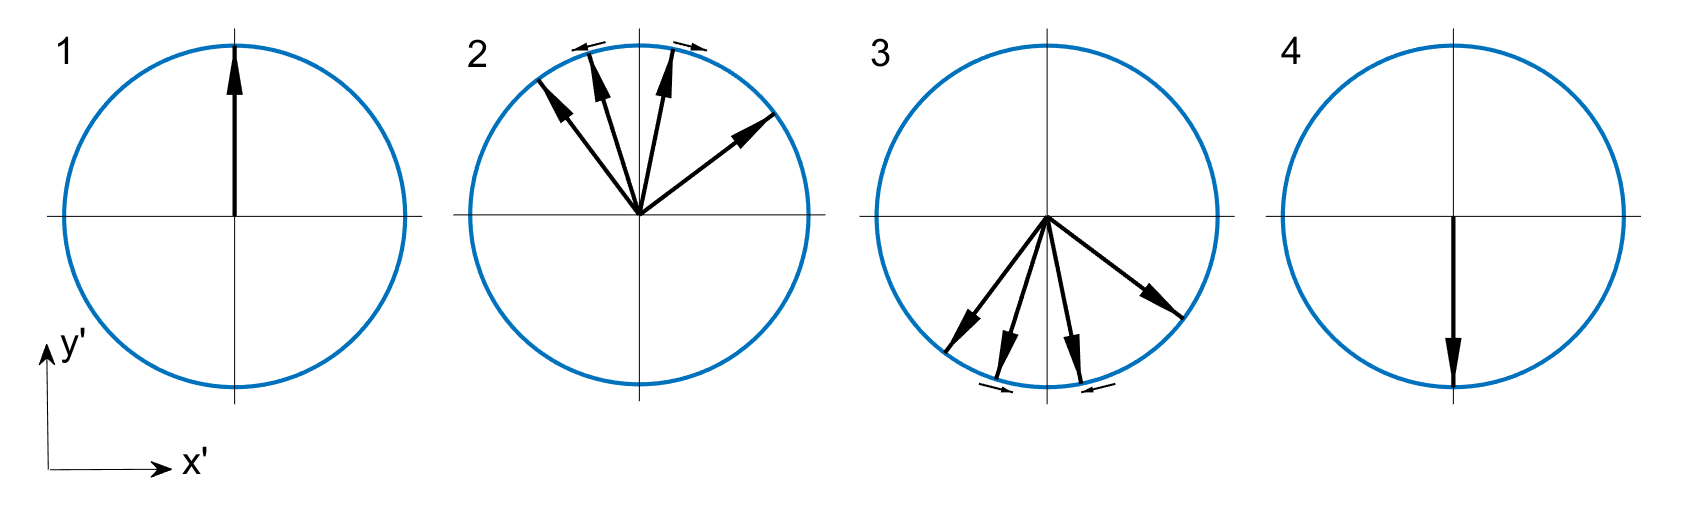
\includegraphics[width = \textwidth]{figures/background/spinecho_evolution.eps}
		\caption{}
		\label{fig:spinecho_evolution}
	\end{subfigure}

	\caption[The spin echo sequence and the evolution of spin under a spin echo sequence.]{a) Spin echo sequence and (b) an indication of the evolution of spins under a spin echo sequence. This shows how the 180\degree\ refocusing pulse acts to refocus the spins after a time $\mathrm{TE}$.}
	\label{fig:spinecho}
\end{figure}
It is possible to undo the effects of $\mathrm{T}_2'$ by designing a pulse sequence to `refocus' the spins, forming what is known as a spin echo.
%Spin echo sequences also enable localisation by combining \ac{RF} pulses with magnetic field gradients.
The first spin echo sequence was introduced by Edwin Hahn in 1950 \cite{Hahn1950}. The simplest sequence to form a spin echo consists of a 90\degree\ pulse to excite the spins followed by a 180\degree\ pulse after a delay. 
This sequence is shown in the diagram in \Cref{fig:spinecho} along with how the signal varies during the pulse sequence.
 
\Cref{fig:spinecho_evolution} represents how the magnetisation evolves through the pulse sequence with the four diagrams corresponding to the points marked in \Cref{fig:spinechosequence}. 
At point 1, immediately following the 90\degree\ pulse, all the magnetisation has been flipped into the transverse plane and is in phase - meaning all the magnetic moments of the spins point in the same direction in the x-y plane. 

The field inhomogeneities cause the different spins to feel slightly different magnetic fields and so precess at slightly different frequencies. 
This causes the spins to lose phase-coherence as indicated at point 2, and so the signal decays with $\mathrm{T}_2^*$.  

At point 3, following the 180\degree\ pulse, the spins remain out of phase with one another, but the 180\degree\ pulse has flipped their orientations across the $x'$-axis. 
The magnetic field the spins feel is still the same, so despite their flip in orientation, they still precess in the same direction. 
This means that the evolution that caused the spins to dephase begins to rewind and bring the spins back into phase coherence. 
After a time equal to the time between the 90\degree\ and 180\degree\ pulses, at point 4, the spins will be brought completely back in phase - or, refocused - and the spin echo is formed. 

The signal at point 4 will still be lower in magnitude than that at point 1 since the $\mathrm{T}_2$ relaxation will still occur as it is an inherent property of the matter. 
The spin echo does, however, refocus the $\mathbf{B}_0$ inhomogeneities. 
The time between the 90\degree\ pulse and the formation of the echo is known as the \ac{TE}. 

The spin echo sequence shown in \Cref{fig:spinecho} forms the basis of the standard \ac{PGSE} diffusion MRI sequence which is introduced in the following section, along with a description of the physics behind diffusion MRI. 

\section{Diffusion MRI}
\label{sec:diffusion_physics}
Diffusion MRI (dMRI) sensitises the \ac{MRI} signal to the motion of water molecules due to diffusion. The following section describes the physics behind diffusion and how the diffusion impacts the \ac{MRI} signal.

% Diffusion MRI simulations attempt to synthesise dMRI signals through models of our understanding of the underlying diffusion processes.
% These simulations broadly fall into two categories: solutions of the diffusion equation and Monte-Carlo simulations of the diffusion dynamics.

% The diffusion equation relates the rate of change of concentration to the spatial variation in concentration according to
% \begin{equation}
%   \frac{\partial c(\vec{r}, t)}{\partial t} = D\nabla^2 c(\vec{r}, t)\,.
% \end{equation}
%Diffusion \ac{MRI} simulations are ultimately trying to synthesise the \ac{dMRI} signal through models of our understanding of the underlying diffusion processes.
%This section briefly covers the physics that gives rise to the \ac{dMRI} signal. 

The diffusion process is driven by the Brownian motion of particles in fluids.
The thermal kinetic energy of particles causes them to move around rapidly, however particles frequently collide with each other (for instance, molecules in water at room temperature experience around 60 billion collisions per second \cite{Denny1993}) creating a very tortuous, random path.

Diffusion \ac{MRI} sensitises the MR signal to this motion by exploiting the dephasing of spins as a result of magnetic field gradients.


The magnetic field will generally have a uniform component from the main $B_0$ field, and spatially and/or time varying components due to deliberate magnetic field gradients or typically unwanted effects such as magnetic susceptibility inhomogeneities and concomitant fields \cite{Haacke1999}. In general, $B(\mathbf{r}, t)$, the magnitude of the magnitude of the magnetic field at a position $\mathbf{r}$ at time $t$ is given by
\begin{equation}
  B(\mathbf{r}, t) = |\mathbf{B}| = |B_0\mathbf{\hat{z}} + \mathbf{\Delta B}(\mathbf{r}, t)|\,,
  \label{eq:mod_B}
\end{equation}
where $\mathbf{\Delta B}(\mathbf{r}, t)$ accounts for all of the variation in the magnetic field away from $B_0$. Note that $\mathbf{\Delta B}(\mathbf{r}, t)$ is a vector quantity which may have components in the $\mathbf{\hat{x}}$ and $\mathbf{\hat{y}}$ directions. 

An idealised expression for $\mathbf{\Delta B}(\mathbf{r}, t)$ often applied to \ac{MRI} assumes that all of the change in the magnetic field is due to an applied magnetic field gradient, $\mathbf{g}(\mathbf{r}, t)$, which only has a significant $\mathbf{\hat{z}}$ component. This means that \Cref{eq:mod_B} can be written as
\begin{align}
  B(\mathbf{r}, t) &= \left|B_0\mathbf{\hat{z}} + \left(\mathbf{g}(\mathbf{r}, t)\cdot\mathbf{r}\right) \mathbf{\hat{z}}\right|\,,\nonumber \\
                      &= B_0 + \mathbf{g}(\mathbf{r}, t)\cdot\mathbf{r}\,.
                        \label{eq:mod_B_ideal}
\end{align}

Magnetic field gradients introduce a deliberate variation in the magnetic field which, according to \Cref{eq:LarmorFreq}, causes the Larmor frequency to vary spatially as well temporally.

Since the Larmor frequency varies spatially, spins in different locations will precess at different frequencies and accrue a phase shift relative to spins in different locations. 
The incremental phase, $d\phi$, accrued for a single spin, $i$, in an infinitesimal time, $dt$, % assuming a gradient in the $z$ direction
is given by
\begin{equation}
  % \phi(t, \mathbf{g}(\mathbf{r}(t), t)) = \gamma B_0 t + \gamma \int_0^t \mathbf{g}(\mathbf{r}(t'), t')\cdot\mathbf{r}(t')dt'\,,
  % \label{eq:phase_singlespin}
  d\phi_i = \gamma B(\mathbf{R}_i(t), t) dt\,,
  \label{eq:dphi}
\end{equation}
% where $\gamma$ is the gyromagnetic ratio, $B_0$ is the main field strength, $\mathbf{r}(t')$ is the position of the particle and $\mathbf{g}(\mathbf{r}(t'), t')$ is the (potentially spatially varying and time-dependent) magnetic field gradient.
where $\gamma$ is the gyromagnetic ratio and  $\mathbf{R}_i(t)$ is the position of the particle at time $t$. %and $B(\mathbf{r}(t), t)$ is the magnitude of the magnetic field at position $\mathbf{r}(t)$ and time $t$.

Putting \Cref{eq:mod_B_ideal} into \Cref{eq:dphi} and integrating over the time of the diffusion experiment will give the total phase accrued for a single spin:
\begin{equation}
  % \phi(t, \mathbf{g}(\mathbf{R}_i(t), t)) = \gamma B_0 t + \gamma \int_0^t \mathbf{g}(\mathbf{R}_i(t'), t')\cdot\mathbf{R}_i(t')dt'\,,
  \phi(\mathbf{R}_i(t)) = \gamma B_0t + \gamma\int_0^t\mathbf{g}(\mathbf{R}_i(t'), t')\cdot\mathbf{R}_i(t')dt'\,,
  \label{eq:phase_singlespin}
\end{equation}


The first term in this equation is the phase accrued due to the main magnetic field which will be the same for all spins in the system.
The second term is the phased accrued due to the gradient, which will be dependent on the motion of each individual spin.
The dot product here indicates that only displacement projected onto the gradient direction affects the phase, allowing the gradient direction to be used to probe the diffusion in different directions.

\begin{figure}
  \centering
  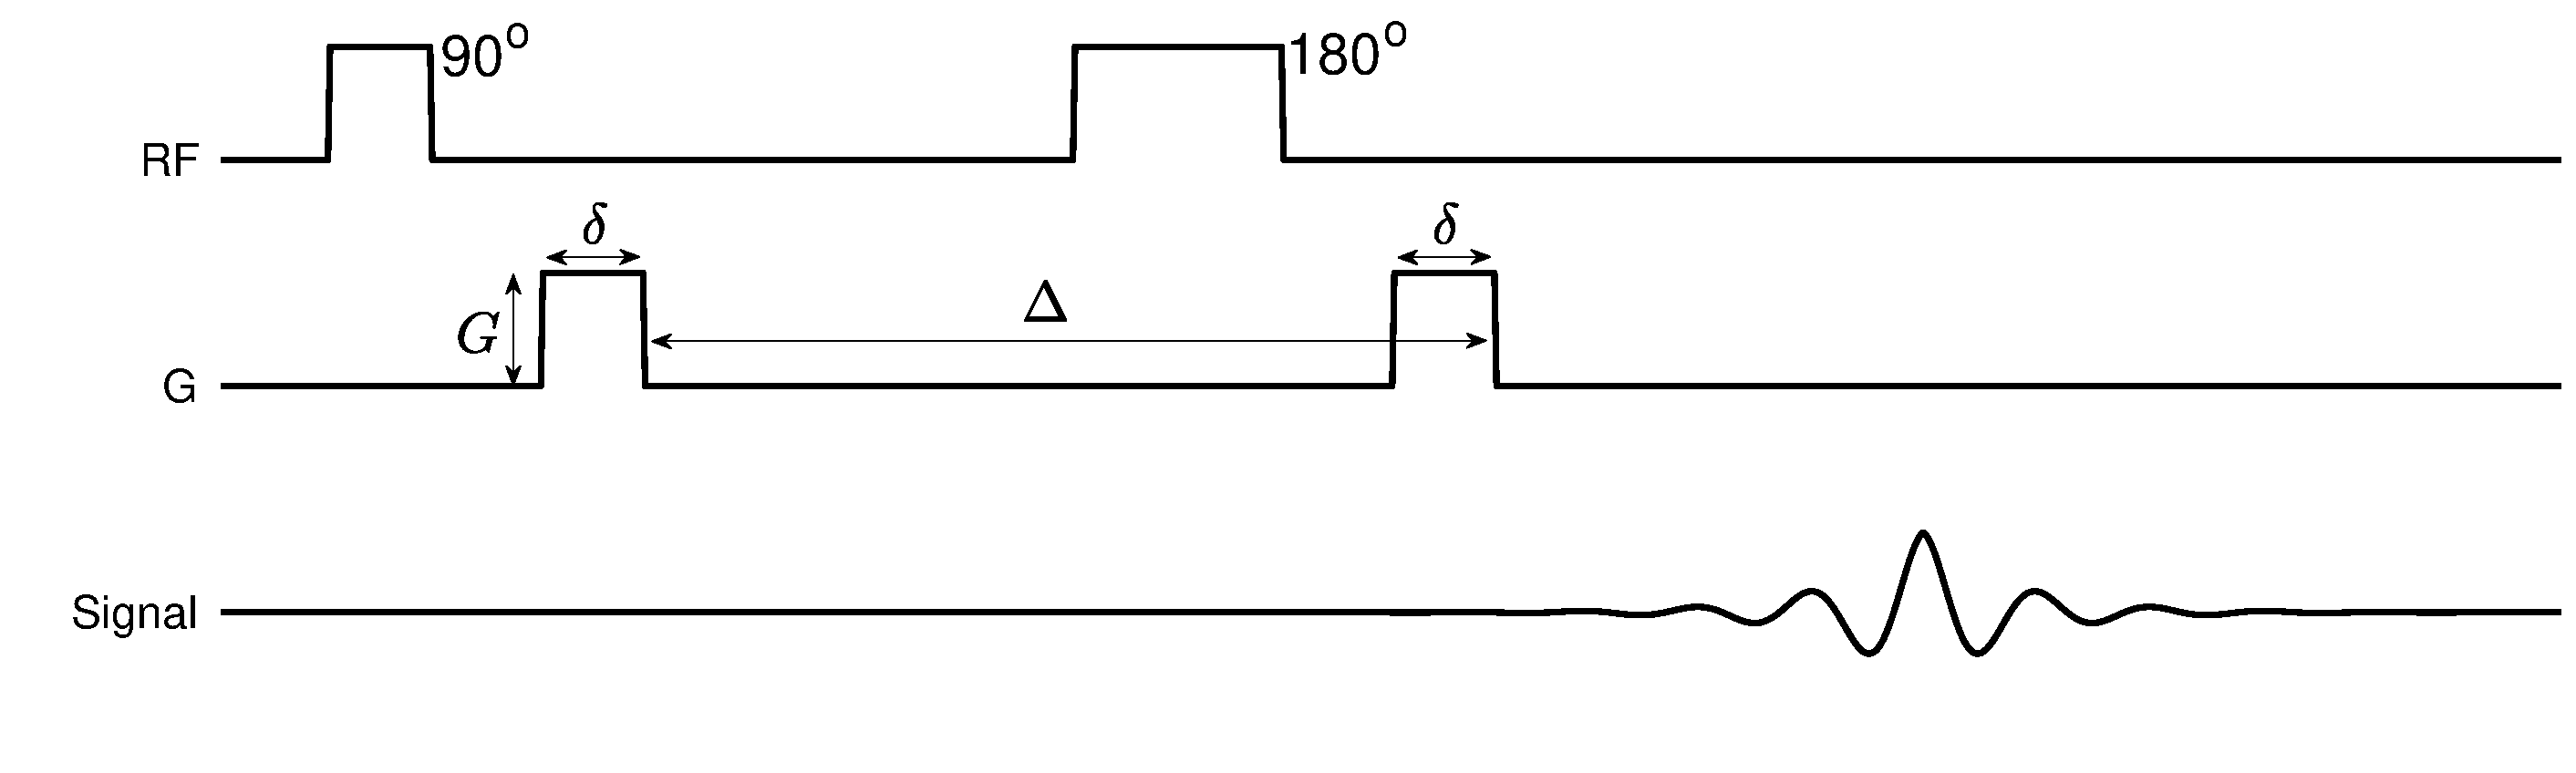
\includegraphics[width=0.9\textwidth]{figures/background/PGSE_diagram.eps}
  \caption{The standard \acl{PGSE} sequence used in \acs{dMRI}.}
  \label{fig:PGSE_diagram}
\end{figure}

The first diffusion MR sequence, introduced by Stejskal and Tanner in 1965\cite{Stejskal1965}, is the \acf{PGSE} sequence, shown in \Cref{fig:PGSE_diagram}.
The PGSE sequence consists of a standard spin echo sequence with a pair of gradient pulses added either side of the refocussing pulse.
In the ideal case, each pulse is rectangular with a gradient strength, $G$, and duration, $\delta$ and they are separated by a time, $\Delta$.  

The effect of this pulse sequence can be simplified by considering the case when $\delta \ll \Delta$. This is known as the \ac{SGP} approximation and means that the motion of spins during the pulses can be ignored. 

Under the \ac{SGP} approximation, the phase accrued by a spin at a position $\mathbf{R}_0$ during a pulse at a time $t_0$ will be
\begin{equation}
  \phi(\mathbf{R}_0) = \gamma B_0\delta +  \gamma \delta \mathbf{g(R_0)}\cdot\mathbf{R_0}\,.
  \label{eq:phi_single_SGP}
\end{equation}
Here, $\mathbf{R}_0$ refers to the spin position at time $t=t_0$ and is not time-dependent, because under the SGP approximation the motion of spins during the pulse is assumed to be negligible. 

The 180\degree\ pulse in the \ac{PGSE} sequence is crucial, since it flips the orientation of the spins' magnetic moments as in the spin echo sequence in \Cref{fig:spinecho}.
Not only does this refocus $\mathrm{T}_2^*$ effects as outlined in \Cref{sec:spin_echoes}, but similarly, it means that the phase accrued due to the first gradient pulse now has a negative sign relative to the phase that will be accrued due to the second pulse. %due to the second gradient pulse has opposite sign to the phase accrued due to the first pulse. 

A spin which is at a position $\mathbf{R}_0$ during the first pulse and then diffuses to a position $\mathbf{R}_1$ during the second pulse will therefore have a relative phase shift of 
\begin{equation}
  \Delta\phi(\mathbf{R}_1 - \mathbf{R}_0) = \gamma\delta\mathbf{g} \cdot \left(\mathbf{R}_1 - \mathbf{R}_0\right)\,.
  \label{eq:delta_phi}
\end{equation}

The $B_0$ term from \Cref{eq:phi_single_SGP} is the same for both gradient pulses, meaning that during the subtraction in \Cref{eq:delta_phi} it cancels and the only relative phase shift comes from the diffusive motion.

The total MR signal comes from an ensemble of spins, each with their own random Brownian motion and thus, from \Cref{eq:delta_phi}, their own relative phase shift.
To get to the total MR signal, we need to consider the probability that a particle starts at position $\mathbf{R}_0$ (i.e. the initial spin density, $\rho(\mathbf{R}_0)$, which can generally be considered uniform within a voxel \cite{Price1997}) and the probability that a particle which starts at $\mathbf{R}_0$ moves to $\mathbf{R}_1$ during the time $\Delta$, $P(\mathbf{R}_0, \mathbf{R}_1, \Delta)$.
Putting these together, gives an expression for the total MR signal\cite{Price1997,Stejskal1965}:
\begin{equation}
  S(\mathbf{g}, \Delta) = S(\mathbf{0}, \Delta)\int\int \rho(\mathbf{R}_0)P(\mathbf{R}_0, \mathbf{R}_1, \Delta) e^{i\gamma\delta\mathbf{g} \cdot (\mathbf{R}_1 - \mathbf{R}_0)}  d\mathbf{R}_0d\mathbf{R}_1\,.
  \label{eq:total_signal_sgp}
\end{equation}

This quantity, $P(\mathbf{R}_0, \mathbf{R}_1, \Delta)$, is known as the diffusion propagator and is of great interest for diffusion MRI because $P(\mathbf{R}_0, \mathbf{R}_1, \Delta)$ encodes the information about the environment in which the spins are diffusing. 
For diffusion in an isotropic, homogeneous medium, the diffusion propagator is a Gaussian distribution \cite{Price1997}:
\begin{equation}
  P(\mathbf{R}_0, \mathbf{R}_1, t) = \left(4\pi Dt\right)^{-\sfrac{3}{2}}\exp\left(-\frac{(\mathbf{R}_1 - \mathbf{R}_0)^2}{4Dt}\right)\,.
  \label{eq:propagator_diffusion}
\end{equation}

In the case of Gaussian diffusion, \Cref{eq:total_signal_sgp} can be solved analytically and will give an MR signal attenuation (that is, $S(t)/S(0)$) which is also Gaussian\cite{Stejskal1965,Price1997}
\begin{equation}
  E(g, \Delta) = \exp(-\gamma^2g^2\delta^2D\Delta)\,.
  \label{eq:sgp_signal_gaussian}
\end{equation}

The general form of this expression, accounting for finite duration gradient pulses, can also be analytically derived to give the Stejskal-Tanner equation \cite{Stejskal1965,Kuchel2012}
\begin{align}
  \ln(E) &= -\gamma^2g^2\delta^2D(\Delta - \delta/3)\,,\label{eq:stejskal_tanner}\\
  &= -bD\,,
\end{align}
where $b = \gamma^2g^2\delta^2(\Delta - \delta/3)$ is the so-called $b$-value which describes the strength of the diffusion encoding. 

We can formulate a more general form of  \Cref{eq:total_signal_sgp} without requiring any assumptions on the gradients (such as the \ac{SGP} approximation used above) as \cite{Price1997,Hall2009}
\begin{equation}
  S(\mathbf{g}, t) = S(\mathbf{0}, t) \int_{-\infty}^{\infty} P(\phi, t) e^{i\phi} d\phi\,,
  \label{eq:sig_phi_complex}
\end{equation}
where the phase, $\phi$ will be given by \Cref{eq:phase_singlespin} and $P(\phi, t)$ is the probability density function of the phase distribution after a time $t$.

In the case of restricted diffusion (i.e.\ diffusion in an inhomogeneous or anisotropic environment) the form of the diffusion propagator becomes more complex and closed form solutions of \Cref{eq:total_signal_sgp,eq:sig_phi_complex} are only possible for certain simple geometries and assumptions.

Analytical solutions can be found for some simple restricting geometries such as spheres, cylinders and parallel plates \cite{Neuman1974, Balinov1993,Callaghan1995}.
For more complex environments, however, an analytical solution is intractable and we must rely on simulations to approximate the \acl{dMRI} signal.  

\begin{comment}
The total MR signal comes from an ensemble of spins, each with their own random Brownian motion and thus, from  \Cref{eq:phase_singlespin}, their own phase. This gives the total \ac{dMRI} signal, $S(t, \mathbf{g})$ as

where $S(t, \mathbf{0})$ is the signal with no gradients applied. $P(\phi, t)$ is the probability density function of the phase distribution after a time $t$.

From \Cref{eq:phase_singlespin}, we see that the individual phases, and thus the phase distribution, depend on the motion of the particles as well as the description of the diffusion sensitising gradient (in the case of standard pulsed gradient experiment that is the timing, strength, duration and orientation of the gradient) \cite{Price1997}.

This quantity, $P(\phi, t)$, is closely related to another property of great interest for diffusion MRI known as the diffusion propagator, $P(\mathbf{R}_0, \mathbf{R}_1, t)$. $P(\mathbf{R}_0, \mathbf{R}_1, t)$ is the probability that a particle initially at a position $\mathbf{R}_0$ moves to $\mathbf{R}_1$ in a time $t$.
For diffusion in an isotropic, homogeneous medium, the diffusion propagator is a Gaussian distribution \cite{Price1997}:
\begin{equation}
  P(\mathbf{R}_0, \mathbf{R}_1, t) = \left(4\pi Dt\right)^{-\sfrac{3}{2}}\exp\left(-\frac{(\mathbf{R}_1 - \mathbf{R}_0)^2}{4Dt}\right)\,.
  \label{eq:propagator_diffusion}
\end{equation}

\end{comment}

\subsection{The \acl{BT} equations}
\label{sec:bg_bloch_torrey}
As well as describing the \ac{dMRI} signal by considering the microscopic diffusion of spins, a macroscopic formulation can be derived considering Fick's laws of diffusion. The combination of the Bloch equations (\Cref{eq:blochx,eq:blochy,eq:blochz}) with Fick's second law of diffusion leads to the \ac{BT} equations, proposed by H.\ C.\ Torrey in 1956\cite{Torrey1956,Callaghan1991,Price2009}:

\begin{equation}
  \frac{\partial\mathbf{M(r},t)}{\partial t} = \gamma \mathbf{M \times B(r}, t) - \frac{M_x\mathbf{\hat{x}} + M_y\mathbf{\hat{y}}}{\mathrm{T}_2} - \frac{(M_z - M_0)\mathbf{\hat{z}}}{\mathrm{T}_1} + \nabla \cdot \left(\mathbf{D} \nabla \mathbf{M}\right)\,.
  \label{eq:bloch_torrey}
\end{equation}

This version of the \ac{BT} equation is sometimes referred to as the standard \ac{BT} equation. An additional term can be added to account for the evolution of the magnetisation due to a flow, described by a velocity field $\mathbf{v}$ to get the generalised \ac{BT} equation \cite{Jeener2002,Beltrachini2016}. However, this flow term is often dropped, assuming no net flow, in the application to \ac{dMRI}, leaving \Cref{eq:bloch_torrey}. 
$\mathbf{D}$ is the diffusion tensor, a generalisation of the diffusion coefficient, $D$, to allow for anisotropic diffusion. In short, this means that diffusion happens at a different rate in different directions.
It is the $\mathbf{D}$ term in \Cref{eq:bloch_torrey} which encodes the evolution of the magnetisation when there is diffusion.

In general, the \ac{BT} equations cannot be solved analytically, apart from in some simple cases such as isotropic free diffusion.
For instance, the solution to the \ac{BT} equations in isotropic free diffusion can be shown to give the expected Stejskal-Tanner equation, \Cref{eq:stejskal_tanner} \cite{Price1997}.

For complex geometries, as with the case above, we must rely on computational methods to come to a solution for the \ac{BT} equations. 



\section{Diffusion Simulation}
\label{sec:diffusion_simulation}
Diffusion simulations attempt to evaluate \Cref{eq:sig_phi_complex} or \Cref{eq:bloch_torrey} computationally. Simulation approaches broadly fall into two categories: numerical solutions of the \ac{BT} equation and \ac{MC} simulations of the diffusion dynamics. This section introduces these techniques, highlighting the some of the similarities and differences between them. 


At a high level, all diffusion simulations have three common components: the substrate, the diffusion dynamics and the measurement.
The substrate describes the environment in which the diffusion is taking place. A common example of this is parallel cylinders representing axons in white matter.
The diffusion dynamics describe our understanding of the processes underlying the diffusive motion of molecules and the measurement describes how this diffusive motion results in a synthetic \ac{dMRI} signal.
\subsection{Numerical solutions}
\label{sec:numerical_solutions}
Numerical solution approaches generally attempt to solve the \acl{BT} equation \cite{Torrey1956}.
These approaches combine both the dynamics and the measurement components of the diffusion simulation by solving for the magnetisation in  \Cref{eq:bloch_torrey}.
The third component, the substrate, defines boundary conditions required for the solution of the equation. 

There are two typical methods for solving the \ac{PDE} in \Cref{eq:bloch_torrey}, \acp{FDM} and \acp{FEM}.
Finite difference methods evaluate the \ac{PDE} using a local Taylor expansion at discrete points which are generally uniformly separated in each spatial as well as the temporal dimension \cite{Grossmann2007}.
\acp{FDM} are an efficient method for solving \acp{PDE} when the problem can fit into a rectangular grid, however they are less effective when applied to complex geometries \cite{Hagslatt2003, Grossmann2007}.

Finite element methods subdivide the domain into small elements which are simple geometric shapes, though unlike the \acp{FDM}, they do not have to form a regular grid, but rather an arbitrary mesh.
In each element, the \ac{PDE} solution is approximated by simple functions such as a linear combination of polynomials.
The combination of all of these local approximations can be solved to give a numerical solution of the \ac{PDE} across the whole domain \cite{Logan2007}.
\acp{FEM} are generally more complex to formulate and implement than \acp{FDM}, however the added complexity can be worth the effort for more difficult problems in which \acp{FDM} may be ineffective \cite{Iserles2009}.

\subsection{Monte-Carlo simulations}
\label{sec:montecarlo}
Monte-Carlo methods take a different approach to the simulation of the \ac{dMRI} signal. Monte-Carlo methods simulate the Brownian motion of a large number of particles, simulating the motion of each particle individually, along with the MR acquisition to generate the \ac{dMRI} signal.

There exist many different implementations of the Monte-Carlo simulation of \ac{dMRI} \cite{Yeh2013,Nilsson2012,Landman2010,Balls2009,Hall2009,Ford1997,Szafer1995}, however the underlying principles are similar for all of them. The following is a general description of the \ac{MC} simulation process, however the specifics for each different implementation may vary. 

% There are three main components of an MC diffusion simulation: (1) the environment in which particles are diffusing (often called the substrate), (2) the dynamics of the Brownian motion and (3) the MR pulse sequence used to acquire the signal. 


Most early \ac{MC} studies used simple, easily parametrised substrates like regularly packed cuboids \cite{Szafer1995} or cylinders \cite{Ford1997}.
As computational power has increased, so too has the capacity for more and more complex substrates.
This includes cylinders with randomly distributed radii \cite{Hall2009}, undulating  cylinders \cite{Nilsson2012}, beading cylinders \cite{Budde2010} and meshes, both generated from high resolution microscopy of tissue \cite{Panagiotaki2010} and computer generated cell models \cite{Palombo2019,Rafael-Patino2018}.

The Brownian motion of particles is typically simulated as a random walk of many independent particles. The time domain is discretised into many time points and at each time point each particle takes a random step through the substrate.  
One step of the random walk can be briefly summarised as shown in \Cref{alg:MC_random_walk}.
\begin{algorithm}
  \begin{algorithmic}
    \State generate randomly oriented step vector
    \State check if step crosses a barrier 
    \While{step crosses barrier}
    \State amend step according to barrier interaction (e.g. elastic reflection)
    \State repeat barrier checking on amended step
    \EndWhile
    \State update the particle position 
  \end{algorithmic}
  \caption{Basic algorithm for taking a step in the random walk.}
  \label{alg:MC_random_walk}
\end{algorithm}
 
Following the Brownian motion, each particle in the simulation will have taken many steps giving each particle a unique trajectory that it has traversed.
The incremental phase, $\Delta \phi$, accrued at each step can be calculated from a discrete version of \Cref{eq:phase_singlespin}. Under the assumption of uniform $B_0$, only the gradient term matters, giving
\begin{equation}
  \Delta \phi = \gamma \mathbf{g}(\mathbf{R}(t), t) \cdot \mathbf{R}(t)\, \Delta t \,,
  \label{eq:deltaPhi}
\end{equation}
where $\Delta t$ is the duration of the step and $\mathbf{g}(\mathbf{R}(t), t)$ and $\mathbf{R}(t)$ are the gradient and particle position during that step respectively.

The phase accumulation in \Cref{eq:deltaPhi} for each spin in the simulation can be combined with \Cref{eq:sig_phi_complex} to approximate the total signal for the \ac{dMRI} acquisition as
\begin{equation}
  S = \sum_j e^{i\Phi_j}\,,
  \label{eq:MCsignal}
\end{equation}
where $\Phi_j$ is the total phase accrued for each spin. 

Monte-Carlo simulations are a powerful tool for \ac{dMRI} simulation due to their ability to handle any arbitrary substrate and MR pulse sequence.
Additionally, \ac{MC} simulations can be modified to account for effects that are more difficult to formulate for analytical and numerical solutions of the diffusion equation such as semi-permeable membranes, membrane-particle interactions and spatially and/or temporally varying $\mathrm{T_1, T_2}$ and diffusivities.

A drawback of \ac{MC} simulation, particularly for complex substrates is the need to simulate enough spins to mimic the ensemble behaviour of spins \emph{in vivo} as well as enough discrete time points to adequately capture the dynamics through the pulse sequence.
The huge number of calculations required to handle large simulations can be alleviated by exploiting the inherent parallel nature of the problem to run simulations in parallel on a \ac{CPU} cluster or, even more effectively, a GPU cluster.

\section{Diffusion Modelling}
\label{sec:bg_diffusion-modelling}
As discussed in \Cref{sec:diffusion_physics}, the environment in which spins diffuse can impact on the diffusion process, imparting information about this environment in the diffusion weighted \ac{MRI} signal via the diffusion propagator. As \ac{dMRI} research has advanced, many works have tried to take advantage of this to estimate information about the cellular environment spins are diffusing to gain biological meaningful information \cite{Novikov2019,Jelescu2017,Alexander2017}.

Broadly speaking, these models fall into two families: signal representations and biophysical models. Signal representations seek to express the signal from a voxel using a general expression which captures salient features of the data without making too many assumptions and by construction don't carry any particular biological meaning \cite{Novikov2019}. Some examples of representations are \ac{DTI}\cite{basserMRDiffusionTensor1994}, \ac{DKI}\cite{Jensen2005} and \ac{DSI}\cite{Wedeen2005}. Biophysical models, however, model tissue by breaking it down into compartments that can be described by simple analytical models such as spheres and cylinders. Some examples of this kind of model are ball-and-stick\cite{Behrens2003}, \ac{CHARMED}\cite{Assaf2005} and \ac{NODDI}\cite{Zhang2012}.

As different models and representations have been proposed over the past two decades, a menagerie of techniques has emerged that is too deep and varied to summarise here, however a number of articles have attempted to review the field \cite{Alexander2017,Novikov2019,Jelescu2017}.
The remainder of this section will briefly cover one family of models that are used in this thesis.

\subsection{Spherical deconvolution techniques}
\label{sec:bg_spherical_deconv}
A popular approach in \ac{dMRI} modelling of brain tissue, in particular \ac{WM}, is to model the signal as a combination of two components: one describing the orientational distribution of the tissue (e.g. direction of axons) and one describing the \ac{dMRI} response of typical tissue (e.g. the typical signal from an axon), sometimes called the kernel.
One such family of techniques, which aims to estimate the orientational distribution of fibres in \ac{WM}, models this relationship as a spherical convolution of the \ac{FOD} with a kernel that is the typical \ac{dMRI} response of a single fibre (or bundle of fibres). This kernel is commonly referred to as the \ac{FRF}.
Mathematically, this is expressed as
\begin{equation}
  S(\theta,\phi) = F(\theta, \phi) \otimes R(\theta) \,,
  \label{eq:bg_sd}
\end{equation}
where $S$ is the \ac{dMRI} signal, $F$ the \ac{FOD}, $R$ the \ac{FRF} and $\theta$ and $\phi$ are the elevation and azimuthal angles respectively. Note here that the \ac{FRF}, $R(\theta)$, is assumed to be axially symmetric. 

Since the goal of these techniques is typically to estimate the \ac{FOD}, the approach is to estimate the \ac{FRF} \emph{a priori} and deconvolve this out to leave the \ac{FOD}.
While there are many techniques based on this \ac{SD} each with slightly different approaches, many such techniques express the signal, \ac{FOD} and \ac{FRF} in their \ac{SH} expansions to facilitate \ac{SD}.

\subsubsection{Spherical harmonics}
\label{sec:bg_spherical_harmonics}
The \acl{SH} series is a spherical analogue to the Fourier series in Cartesian space, providing an orthonormal basis of functions on the sphere which can be used to represent any spherical function.
The basis functions are denoted $Y_l^m(\theta, \phi)$ where $l$ is called the degree and $m$ the order of the \ac{SH}. Any (potentially complex valued) function, $f$, on the sphere can then be written as a linear combination of \acp{SH}:
\begin{equation}
  f(\theta, \phi) = \sum_{l=0}^\infty \sum_{m=-l}^l c_l^m Y_l^m(\theta, \phi) \,,
  \label{eq:bg_sh}
\end{equation}
where the \ac{SH} coefficients, $c_l^m$, are given by
\begin{equation}
  c_l^m = \int_0^{2\pi} \int_0^\pi f(\theta, \phi) Y_l^{m*}(\theta, \phi) sin(\theta) d\theta d\phi\,,
\end{equation}
where $*$ denotes complex conjugation.

The benefit of working in \acp{SH} is that the spherical convolution in \Cref{eq:bg_sd} simplifies to a set of matrix multiplications in spherical harmonics:
\begin{equation}
  \vec{S}_l = R_l \vec{F}_l\,,
  \label{eq:bg_sd_matrix}
\end{equation}
where $\vec{S}_l$ is the $2l + 1$ vector of $l^{\mathrm{th}}$ degree \ac{SH} coefficients of the signal, $\vec{F}_l$ is similarly the $l^{\mathrm{th}}$ degree \ac{SH} decomposition of the \ac{FOD} and $R_l$ is the $(2l+1)(2l+1)$ matrix representing the $l^{\mathrm{th}}$ degree rotational harmonic decomposition of the \ac{FRF}.
$R_l$ must be represented by rotational harmonics (an analogue of the Fourier series in $SO(3)$ rather than $S^2$ as with \ac{SH}) for this to work mathematically \cite{Healy1998,Tournier2004} however much of the complexity is simplified due to the physical properties of the \ac{dMRI} signal.

Firstly, the assumption that the \ac{FRF} is axially symmetric means that the $R_l$ collapses to a single scalar value for each $l$ \cite{Tournier2004}, making the solution of \Cref{eq:bg_sd_matrix} for $\vec{F}_l$ a simple case of the division of $\vec{S}_l$ by a scalar. Secondly, since the \ac{dMRI} signal is antipodally symmetric, all odd $m$ terms are zero and since it's real valued, the \ac{SH} coefficients exhibit conjugate symmetry, that is $c_l^m = (-1)^mc_l^{-m*}$ \cite{Tournier2004,Alexander2002}.

All of this means that \ac{SD} based techniques are efficient methods to estimate the \ac{FOD} from \ac{dMRI} and as such have been used in many studies to investigate the organisation and structural connectivity of the brain \cite{DellAcqua2019,Schilling2019,Raffelt2012,Tournier2007,Tournier2004,Schilling2019b,Maier-Hein2017,Neher2014a,Jbabdi2011}.
These techniques will, of course, depend on the \ac{FRF} which is estimate prior to performing the spherical deconvolution, something which we investigate in \Cref{chap:frf_experiment}. 
\begin{comment}
\section{Neural growth}
\label{sec:bg_nerual_growth}
Neural development is a complex and constantly evolving field of research, due in part to the sheer size and complexity of the fully developed brain - for instance, during human development about 100 billion cells are generated with about 100 trillion connections between them \cite{Price2017}. This means that development on an individual neuron basis can only be studied in simple organisms with only a few hundred neurons and even then there are many mechanisms which are yet to be fully understood \cite{Price2017}.

In spite of this, many neural growth mechanisms have been identified and studied in simple organisms and \emph{in vitro} experiments \cite{Price2017,Rauch2013,Nikic2011,Dent2011,Polleux2010,Lowery2009,Mortimer2008,Sakisaka2005,Scott2001,NAP1785} which give us some understanding of how neurons take their shape.

At this point, a brief review of some biological terms that will be used extensively is useful.
Firstly, brain cells can broadly be split into two categories: neurons and glial cells.
Neurons are the cells which transmit and receive signals within the brain and between the brain and the rest of the body.
Neuronal cells can be thought of in a few parts, firstly the cell body, or soma, contains the nucleus of the cells, secondly long extensions known as neurites grow out from the soma.
Neurites themselves are broken down into either dendrites or axons.
A neuron typically has a single axon which is a long neurite which carries information away from the soma while the dendrites form a branched tree which integrates incoming information to the neuron \cite{Price2017}.
Glial cells perform many functions which enable the nervous system to function efficiently such as creating the myelin sheaths which cover the axons to facilitate fast and efficient transmission of signals.

On a higher level, the brain can broadly be split into two types of tissue, \acf{WM} and \acf{GM}. Grey matter contains the majority of the neuronal cell bodies in the brain while the \acl{WM} is typically composed of primarily axons connecting different \ac{GM} regions together. It is the \acl{WM} which is of interest for this work, so it is important to understand how axons grow to understand how the \ac{WM} is organised.

\subsection{Axonal growth mechanisms}
\label{sec:bg_axonal_growth}
Axons grow by following chemical cues in their environment which are detected by the so-called growth cone at the tip of the axon.
The growth cone is a set of finger- and sheet-like outgrowths which explore the environment surrounding the tip of the axon to drive the growth of the axon\cite{Price2017}.
Whilst not fully understood, there are a number of proposed mechanisms by which the growth cone interacts with its surroundings guide axonal growth. The remainder of this section will outline some of the prominent growth mechanisms.
\end{comment}


%%% Local Variables:
%%% mode: latex
%%% TeX-master: "../main"
%%% End:

\chapter{Literature Review}
\label{chap:literature_review}

\chaptertoc{}

\begin{chapterabstract}
  This chapter presents some examples of the use of numerical phantoms from literature.
  It represents a review of the contemporary literature in \ac{dMRI} simulation, highlighting the state of the art and presenting some weaknesses which this project aims to address. 
\end{chapterabstract}




% \subsection*{Analytical Solutions}
% As mentioned in Section \ref{sec:analytical}, analytical approaches are limited in terms of the geometrical complexity that they can capture.
% The hybrid method of Rensonnet et al.\ is an approach that takes advantage of the convenience of analytical solutions in simple geometries and the flexibility of MC simulations in more complex geometries.
 

\section{Numerical Solutions}
\label{sec:app_numerical_solutions}
Many of the studies presenting a numerical solution are focused on the validation of the technique and improvements to various algorithms rather than the direct use of the technique involving numerical phantoms.

One application of \ac{FDM} solutions of the Bloch-Torrey equations is in the simulation of \ac{dMRI} signals from histological images.
For example, Chin et al.\ \cite{Chin2002} simulate the signal from segmented histological images of mouse spinal cord white matter, showing that the fast and slow components of a biexponential decay of diffusion attenuation do not arise from a contribution from each of the intra and extracellular components.
Hwang et al.\ \cite{Hwang2003} extend this technique to 3D, showing that their \ac{FDM} solutions agree well with analytical solutions for hexagonally packed cylinders. 

Xu et al.\ \cite{Xu2007} develop a matrix based \ac{FDM}, also testing their solution on hexagonally packed cylinders, showing a reduction in error compared to a conventional FDM.
This \ac{FDM} is used by the same group to investigate the sensitivity of \ac{dMRI} to intracellular structure \cite{Xu2009}.
A numerical phantom of cells represented as densely packed spheres with spherical nuclei at the centre of each sphere.
The FDM is used to show that an \ac{OGSE} sequence is more sensitive to changes in the nucleus size than a \ac{PGSE} sequence.
Similarly, Xu et al.\ \cite{Xu2014} use histology based \ac{FDM} simulations to investigate the efficacy of an axon diameter technique based on an \ac{OGSE} sequence. They show that the \ac{OGSE} technique is able to distinguish axons of a lower diameter than traditional \ac{PGSE} techniques. 

% Most studies presenting an FEM solution are focused on the validation of the technique rather than the application of the technique and its use in numerical phantoms.
% Hagsl\"att et al. \cite{Hagslatt2003}, Moroney et al. \cite{Moroney2013}, and Beltrachnini et al. \cite{Beltrachini2016} all show an effective implementation of an FEM solution with various improvements in the stability and accuracy of the solutions.
% Van Nguyen et al.\ \cite{Nguyen2014} implement a 3D FEM solution of the Bloch-Torrey equation and apply it to three example questions in dMRI.
% \todo{add more on numerical solutions}
The first example of an \ac{FEM} solution known to the author is presented by Hagsl\"att et al.\ \cite{Hagslatt2003}.
In this study, rather than solving the \ac{BT} equation, the \ac{FEM} is used to solve for the diffusion propagator \cite{Callaghan1991,Price1997}. From the diffusion propagator, the diffusion attenuated signal is calculated based on an assumption of infinitely narrow gradient pulses.
A good agreement is shown between simulation and theoretical solutions for a range of simple geometries (parallel plates, a lamellar system and  hexagonally packed cylinders).

More studies have recently begun investigating diffusion simulation using \acp{FEM}.
Moroney et al.\ \cite{Moroney2013} present an \ac{FEM} solution of the \ac{BT} equation without the relaxtion and flow terms for numerical analysis of \ac{dMRI} experiments in the short gradient pulse limit. \ac{FEM} results are compared to analytical solutions and \ac{MC} simulations in simple geometries, showing that the \ac{FEM} is more accurate than \ac{MC} simulations, whilst taking less time to run.

Nguyen et al.\ \cite{Nguyen2014} also present an \ac{FEM} solution of the standard \ac{BT} equation, showing its application to diffusion simulation with more general gradient waveforms.
The \ac{FEM} solution is shown to be more accurate in some simple geometries than a finite volume method, with second order accuracy in both the spatial and temporal domains.
Three example applications to questions in \ac{dMRI} are demonstrated using this \ac{FEM}
\cite{Nguyen2014}.
One shows that an infinitely thin membrane can be used to approximate a thick membrane. The second shows that the \ac{ADC} approaches the value predicted by mathematical homegenisation for long diffusion times. Finally, a model of a neuron is presented as a spherical body, with cylindrical axons and dendrites potruding. The \ac{ADC} is shown to approach a steady state faster with a smaller neuronal body.

Beltrachini et al.\ \cite{Beltrachini2016} present a solution of the generalised \ac{BT} equation, extending the \ac{FEM} of Nguyen et al.\ \cite{Nguyen2014} to include the relaxation and flow terms. This \ac{FEM} improves on some of the restrictions in the \ac{FEM}, making the simulations more stable through the use of an implicit scheme that is stable for coarser discretisations without compromising the validity of the result. 


\section{Monte-Carlo - Packages}
\label{sec:app_monte_carlo_packages}
Historically, most studies utilising \ac{MC} simulation used in-house developed \ac{MC} simulation software \cite{Lipinski1990, Szafer1995,Stanisz1997, Duh2001}, however in more recent years and as the complexity of situations possible to simulate has grown, a range of \ac{MC} simulation packages have been released for public use.

Hall and Alexander \cite{Hall2009} introduced \ac{MC} simulation as part of the Camino diffusion MRI toolkit \cite{Cook2006} in the context of simulating swelling cylinders as a model of the effect of ischaemic stroke, however the \ac{MC} framework is very general and can be used to simulate any arbitrary substrate from simple geometric constructs to complex 3D meshes. 

Balls and Frank \cite{Balls2009} present DiffSim, a dMRI simulation framework which embeds the MCell \cite{Stiles1996,Stiles2001, Kerr2008} cellular microphysiology simulator within an \ac{MRI} simulator for synthesising the \ac{dMRI} signal.
DiffSim is used to simulate myelinated white matter \cite{Baxter2013}, showing that an analytical solution model by Sen and Basser \cite{Sen2005} holds for an \ac{SGP} approximation or long diffusion time, however with more realistic pulse sequence parameters, the numerical simulations show lower anisotropy than the analytical model. 

Landman et al.\ \cite{Landman2010} developed the DW-MRI \ac{RWS} showing, as an example of its flexibility and reproducibility, a range of geometrical models for white matter damage, including healthy straight cylinders, bulging cylinders, crimped cylinders and broken cylinders.

Yeh et al.\ \cite{Yeh2013} present \ac{DMS}, showing a range of diffusion substrates ranging from simple parallel uniform cylinders to more complex undulating, beading or crossing arrangements of fibres.
A recent extension of \ac{DMS} shows more complex white matter numerical phantom including orientation dispersion, tortuosity, beading and nodes of Ranvier \cite{Ginsburger2018}, however the range of orientation dispersion and axon densities achieved does not reach typical \emph{in vivo} values.
As of the writing of this review, the \ac{DMS} software package has not been publicly released. 

\section{Monte-Carlo - Numerical Phantoms}
\label{sec:app_monte_carlo_numerical_phantoms}
The above packages, as well as \ac{dMRI} simulation software developed in-house in various research groups, have been used to investigate the diffusion signal in many different numerical phantoms. 

A common target of microstructure imaging is the estimation of axonal diameter and density.
As mentioned above, \ac{FDM} approaches have been used to investigate this \cite{Chin2002,Xu2014}, whilst this has been the subject of \ac{MC} simulation studies as well.
Alexander et al.\ \cite{Alexander2010} use Camino to simulate a series of numerical phantoms of parallel cylinders with radii drawn from a Gamma distribution for the validation of a technique for orientationally invariant indices of axon diameter and density.

Recently Nilsson et al.\ \cite{Nilsson2017}, investigated the theoretical resolution limit for cylinder diameter estimation using diffusion MRI. Analytic expressions based on the Gaussian phase distribution approximation \cite{Price1997} were used for the intracellular signal and validated with \ac{MC} simulations to determine a $d_{min}$, the diameter below which a cylinder cannot be differentiated from a cylinder with diameter approaching zero. The resolution limit for clinical scanners was found to be between 4 - 8 $\mu$m.
This suggests a limitation on the level of microstructural detail that can be estimated using current clinical \ac{MRI} machines.

% Zhang et al.\ \cite{Zhang2011} extend this technique to include orientation dispersion, and then refine the technique to only estimate neurite orientation dispersion and density (NODDI) \cite{Zhang2012}. All of these techniques are validated using MC simulations on numerical phantoms of cylinders with varying densities and orientation dispersion introduced.\todo{make sure this actually true} 

Another problem commonly investigated using numerical phantoms is that of exchange between the intra and extracellular compartments of tissues.
Permeability is difficult to control and vary in physical or biological phantoms, so numerical phantoms offer a unique tool with which to explore permeability and exchange models.

Nilsson et al.\ \cite{Nilsson2009, Nilsson2010} and Fieremans et al.\ \cite{Fieremans2010} investigate the K\"arger model \cite{KARGER1988}, a model for exchange between two signal bearing compartments.
These three studies all use similar numerical phantoms made of straight cylinders in which there is some probability that on encountering a barrier, the spin will pass through the barrier, exchanging spins between the compartments.

In their first study, Nilsson et al.\ \cite{Nilsson2009} use simulations and experimental data to draw the conclusion that it is necessary to include exchange in a model containing two compartments, one of which is restricted. 
Fieremans et al.\ \cite{Fieremans2010} show that the K\"arger model is able to describe the signal for long diffusion times and sufficiently impermeable membranes, however at larger permeabilities, the K\"arger model underestimates the value of the permeability.
Nilsson et al.\ also investigate the effectiveness of the K\"arger model at estimating the intracellular water fraction, showing that the K\"arger model has a negative bias, underestimating the intracellular water fraction by up to 25\% when there is high permeabilty when compared to a computational model made by building a database of simulated signals \cite{Nilsson2010}.
% These studies suggest that the simple K\"arger model is sufficient to explain the dMRI signal in certain situations, however in general it is in sufficient.

Nilsson et al.\ \cite{Nilsson2012} also investigate the importance of axonal undulation on diffusion MRI measurements.
In this experiment, numerical phantoms consisting of axons with either sinusoidal or helical undulations were used in \ac{MC} simulations to investigate the impact on a range of \ac{dMRI} measured parameters.
Nilsson et al.\ show that undulation affects essentially all of the parameters they tested derived from \ac{dMRI}, for instance, undulation results in an overestimation of axonal diameter when using models that assume axons are straight \cite{Nilsson2012}. 

Budde et al.\ \cite{Budde2010} use \ac{MC} simulations to investigate the effect of neurite beading, showing that beading is sufficient to explain the decrease in \ac{ADC} after ischaemic stroke. Numerical phantoms consisting of straight cylinders with increasing amounts of beading introduced are simulated, showing a decrease in \ac{ADC} in both the intra and extracellular spaces with increased beading. 

Lin et al.\ \cite{Lin2016} investigate the effect of \ac{TBI} on \ac{dMRI} derived parameters.
Using a numerical phantom consisting of straight cylinders representing axons and ellipsoids representing glial cells, the effects of \ac{TBI} are investigated by varying various parameters such as the size of the glial cells, the permeability of the cylinders and the spacing of the cylinders \cite{Lin2016}. 
Using this technique, Lin et al.\ conclude that the inconsistencies amongst previous \ac{dMRI} based \ac{TBI} studies \cite{Huisman2004,Bazarian2007,Rutgers2008} are due to differences in the timing between the onset of \ac{TBI} and the diffusion measurement, arguing that different processes drive the \ac{TBI} at different timings, leading to different \ac{dMRI} characteristics. 

Lin et al.\ \cite{Lin2017} similarly investigate the effect of myelin water exchange on various \ac{dMRI} derived parameters. In this work, their representation of \ac{WM} is slightly different, choosing nested cylinders to represent the intra-axonal and myelin-water compartments.
Using \ac{MC} simulations on these cylinders, they show correlations between \ac{dMRI} derived parameters such as \ac{ADC} and \ac{FA} and the \acl{TE}.

Lam et al.\ \cite{Lam2015} produce an empirical model of the extra axonal space using a series of \ac{MC} simulations based on both regularly and randomly packed cylinders. The model is based on the diffusion spectrum \cite{Stepisnik1993}, modelling diffusion in densely packed cylinders as diffusion in a series of pores with a small chance of exchange between the pores.
The empirical model agrees closely with \ac{MC} simulated data.

Some studies combine analytical solutions of the Bloch-Torrey equation and \ac{MC} simulations.
Rensonnet et al.\ \cite{Rensonnet2015} use this combined simulation to synthesise signals for parallel and crossing cylinders.
The intracellular component is modelled using an analytical solution for diffusion within a cylinder based on Grebenkov's multiple correlation function approach \cite{Grebenkov2008}.
The extracellular compartment, which is much more complex geometrically, is simulated using Monte-Carlo simulations.
This hybrid approach yields simulation results which are indistinguishable from pure \ac{MC} simulation whilst being quicker and more precise than a purely \ac{MC} approach \cite{Rensonnet2015}. 

In a further study, Rensonnet et al.\ \cite{Rensonnet2017} use this approach to assess the validity of the superposition approximation of crossing fascicles (i.e. that the total signal from crossing fascicles is the sum of the signal from each fascicle independently).
They are able to show that the signal differences between the superposition approximation and a full simulation of interwoven fascicles is small enough compared to typical noise levels in clinical \ac{dMRI} data, that the superposition approximation is sufficient to describe the signal.
A drawback to this hybrid approach is that the intra and extracellular compartments are treated as distinct, non-interacting compartments, meaning that membrane permeability is not accounted for.

An emerging application for \ac{dMRI} simulations in the direct computational modelling of microstructure.
The first example found for this type of modelling is actually the 2010 work by Nilsson et al. \cite{Nilsson2010} mentioned above for evaluating the K\"arger model.
In recent years however, this idea has reemerged, partially thanks to the popularity of machine learning and emergence of MR fingerprinting.

One area of application these approaches have found is in the estimation of axonal permeability. Nedjati-Gilani et al.\ \cite{Nedjati-Gilani2017} use a machine learning technique known as random forest regression to learn the relationship between \ac{dMRI} signal and microstructural parameters. They simulate diffusion using Camino in a range parallel cylinder substrates with different microstructural parameters including membrane permeability to build a dataset to train the random forest regression.
The random forest regression is shown to estimate membrane permeability well, performing better than the K\"arger model and an application to \ac{MS} is presented, showing \emph{in vivo} results consistent with pathology.

Palombo et al.\ \cite{Palombo2018a} verify this method using a cuprizone treated \emph{in vivo} mouse model. Cuprizone is a well known mouse model of \ac{WM} demyelination, which is important as demyelination is hypothesised to affect axonal permeability.
The random forest approach achieves accurate and robust estimation of microstructural parameters which match expected microstructure changes from electron microscopy and gains more specific information that typical \ac{dMRI} measures such as \ac{ADC} and \ac{FA}. 

Hill et al.\ \cite{Hill2018} extend this work to use a deep \ac{NN} in place of the random forest regression. They are able to show that the \ac{NN} outperforms the random forest approach and an application in \emph{in vivo} mice estimates microstructural parameters in the biologically plausible range.

Rensonnet et al.\ \cite{Rensonnet2018} also attempt to use computational models to directly estimate microstructural parameters using \ac{dMRI} simulations.
Using the hybrid approach mentioned above \cite{Rensonnet2015}, they generate a dictionary of \ac{dMRI} simulation signals for various combinations of microstructural parameters and crossing fascicles.
Measured signals are then compared against this dictionary to find the entry that most closely matches the measured signal to get an estimate of the microstructural parameters.
They show that their approach achieves accurate and robust estimates of microstructural parameters and shows good correspondence with histology compared to traditional closed-form models when applied to an \emph{in vivo} mouse model of spinal cord injury. 



\section{\ac{GPU} accelerated \ac{MC} simulations}
\label{sec:review_gpu}
There have been a couple of studies attempting to modify \ac{MC} \ac{dMRI} simulations for the \ac{GPU}.
The first, by Waudby and Christodoulou \cite{Waudby2011} implements a simple random walk on the \ac{GPU}, with a rejection sampling scheme to handle substrate boundaries.
In this case, a step crossing a boundary is ignored and no step is taken rather than being reflected.

Unlike other geometries studied in this report, the Waudby and Christodoulou work uses a binary representation for simple shapes, meaning that the collision check is as straightforward as checking whether a spin moves into a region of space that is disallowed.
One downside of this approach is that complex geometries cannot be easily represented in this binary manner.

Waudby and Christodoulou show that the \ac{GPU} implementation is able to replicate unoptimised \ac{CPU} and analytical solutions for simple geometries whilst achieving a 1000$\times$ speedup over the \ac{CPU} implementation.
It is mentioned, that with \ac{CPU} optimisation, this difference should reduce to around 20$\times$.

A second, more recent, \ac{GPU} accelerated \ac{dMRI} simulation has been reported by Nguyen et al.\ \cite{Nguyen2018}.
This implementation handles arbitrary meshes with two approaches, one with an octree acceleration scheme and one following a similar binary approach to Waudby and Christodoulou.
The octree scheme gives them a 45-65$\times$ acceleration over Camino with the binary \ac{GPU} version achieving a 2000$\times$ acceleration.
The binary representation in this work uses a uniform grid to divide the space.
Each cell in the grid is assigned a 1 or a 0 based on whether or not it is inside the mesh and a step is considered to have collided with the mesh if it steps from a cell with a 1 to a cell with a 0.

This approach enables them to achieve a massive speedup in their simulation, however, it is limited by the resolution of the grid and the size of the smallest features in the mesh.
Nguyen et al.\ show that if the resolution is not sufficient, the simulated signal will not accurately represent the signal from the true mesh.
For relatively small substrates, this is not a problem as the grid can be made fine enough, however for large and complex substrates, the memory requirements may become excessive.

Currently, the \ac{GPU} \ac{dMRI} simulator presented by Nguyen et al.\ is not publicly available. 


\section{Conclusions}
\label{sec:review_conclusions}
There has been significant work into the use of numerical phantoms in the simulation of \acl{dMRI} signals.
One thing which is common throughout most of the works is a simple model of \ac{WM}.
Typically, \ac{WM} is represented as a set of densely packed, straight, parallel cylinders, which oversimplifies the underlying complexity of the microstructure.
Lee et al.\ \cite{Lee2018a} use electron microscopy to reconstruct a 3D section of mouse corpus callosum, showing that real \ac{WM} contains a large amount of microstructural complexity, including orientation dispersion, undulation and diameter variations.

Generating \ac{WM} substrates which accurately represent real microstructure is important for the kinds of model validation studies mentioned in \Cref{sec:app_monte_carlo_numerical_phantoms} because if a model is validated using overly simplified simulations, it may not be very robust when applied to real data.

Realistic \ac{WM} representations are important for the kind of computational models mentioned in \Cref{sec:app_monte_carlo_numerical_phantoms} for similar reasons.
Another element which is particularly important for building the training datasets or dictionaries for these kinds of computational models is controllability.
The \ac{WM} numerical phantoms need to be realistic, but also must be able to be generated in a controlled manner so that we can generate substrates covering the relevant ranges of microstructural parameters needed to build robust computational models.

These are the main driving reasons behind the work presented in \Cref{chap:config} which aims to build these realistic \ac{WM} substrates with controllable morphology.


%%% Local Variables:
%%% mode: latex
%%% TeX-master: "../main"
%%% End:


\part{Methods Development}
\label{part:methods-development}
\chapter{Fibre Growth for WM numerical phantom generation}
\label{chap:ipmi-implementation}

\chaptertoc{}

\begin{chapterabstract}
  This chapter introduces a preliminary fibre growth algorithm (\acused{preFiG}\ac{preFiG}), a method for generating \acf{WM} numerical phantoms with realistic orientation dispersion and packing density.
  The growth algorithm is introduced, describing how each \ac{WM} fibre is grown individually to generate a densely packed substrate.

  Some experiments are presented, one of which explores how different inputs to \ac{preFiG} impacts the shape of resulting fibres.
  An application of the method to dMRI is demonstrated with simulations of the diffusion-weighted MR signal in three example substrates with differing orientation dispersions, packing densities and permeabilities.
\end{chapterabstract}


\section{Introduction}
\label{sec:Introduction}
Numerical phantoms have found much use for validating many magnetic resonance imaging (MRI) experiments.
In particular, numerical phantoms are often used when developing diffusion MRI (dMRI) microstructure imaging techniques where simulations of the dMRI signal in phantoms with known microstructural properties are used in lieu of an in vivo ground truth measure of microstructure \cite{Alexander2017}.

While recently numerical phantoms have proven useful for validating microstructure imaging of grey matter \cite{Palombo2020}, they have more commonly been used for validating white matter (WM) microstructure, with many studies comparing parameter estimates from fitting their models to the known ground truth from the phantoms e.g. \cite{Li2019,Jelescu2017,Scherrer2016,Tariq2016,Daducci2015,Nilsson2017,Xu2014,Zhang2012,Nilsson2010}.
Some recent works directly estimate microstructural features using fingerprinting techniques and machine learning to match simulated signals and the corresponding ground truth microstructure of the numerical phantom to the measured signal\cite{Hill2019,Palombo2018a,Rensonnet2018,Nedjati-Gilani2017}.
As well as affecting the dMRI signal, microstructural features also influence other MR techniques such as susceptibility-weighted imaging \cite{Li2012,Lee2010}.
For instance, Xu et al. \cite{Xu2018} recently used simulations to show that using realistic axonal models rather than simple circular cylinders affects the MR signal.
Therefore, it is important to the MRI community to generate realistic WM numerical phantoms which accurately capture microstructural features in order to get realistic simulated signal.

Generating realistic WM numerical phantoms which accurately capture realistic microstructural features (such as dispersion, undulation, beading, etc.) at high packing densities is a major open challenge for the dMRI community.
While densely packing straight, parallel, fibres is relatively easy, only a few groups have attempted to densely pack irregular, non-parallel, fibres.

The most common approach to this is the packing of fibres into densely packed configurations \cite{Close2009,Ginsburger2018,Ginsburger2019,Rafael-Patino2018}.
The typical approach, as taken in the state-of-the-art MEDUSA algorithm \cite{Ginsburger2019}, is to generate a set of overlapping fibres decomposed into small segments and iteratively refine their positions to remove the overlap between them.
Despite their recent progress, further advance of this class of techniques may be limited, because nature does not create fibres before attempting to pack them together.
Instead, real axons are guided by chemical cues and fit into available space as they grow \cite{Price2017,Lowery2009}.
Mimicking the natural fibre genesis may prove important for building more realistic phantoms.

Here, we propose a completely different strategy: rather than densely `packing' irregular fibres, we `grow' fibres contextually, mimicking natural fibre genesis.
We propose a preliminary fibre growth algorithm (\ac{preFiG}) for the generation of WM numerical phantoms with more realistic orientation dispersion and packing density.
Fibres are grown one-by-one following a cost function which attempts to impose the morphological priors that are input to the algorithm.

The rest of the chapter is organised as follows: \Cref{sec:ipmi_config_description} describes \ac{preFiG}, \Cref{sec:impi_experiments_and_results} details some experiments showing the potential of the algorithm and comparing it to a brute-force approach to fibre growth and \Cref{sec:ipmi_discussion} summarises the contributions and discusses limitations in the preliminary implementation and future work to improve the method.


\section{A preliminary fibre growth algorithm}
\label{sec:ipmi_config_description}
In this section we describe a preliminary fibre growth algorithm (\acs{preFiG}) which grows fibres one-by-one avoiding intersection between fibres whilst attempting to ensure that the resulting substrate has desired morphological input properties such as orientation dispersion, diameter distribution and packing density.

The generation of \ac{preFiG} numerical phantoms happens in three main steps:
\begin{description}
  \item [STEP 1] \label{item:step1} Generate initial growth configuration from user inputs
  \item [STEP 2] Grow the fibres using \ac{preFiG} growth algorithm
  \item [STEP 3] Generate 3D meshes for dMRI simulation
\end{description}

The remainder of this section outlines these steps in further detail, breaking each step down into smaller steps and detailing each one in further detail. 

\begin{figure}[t]
  \centering
  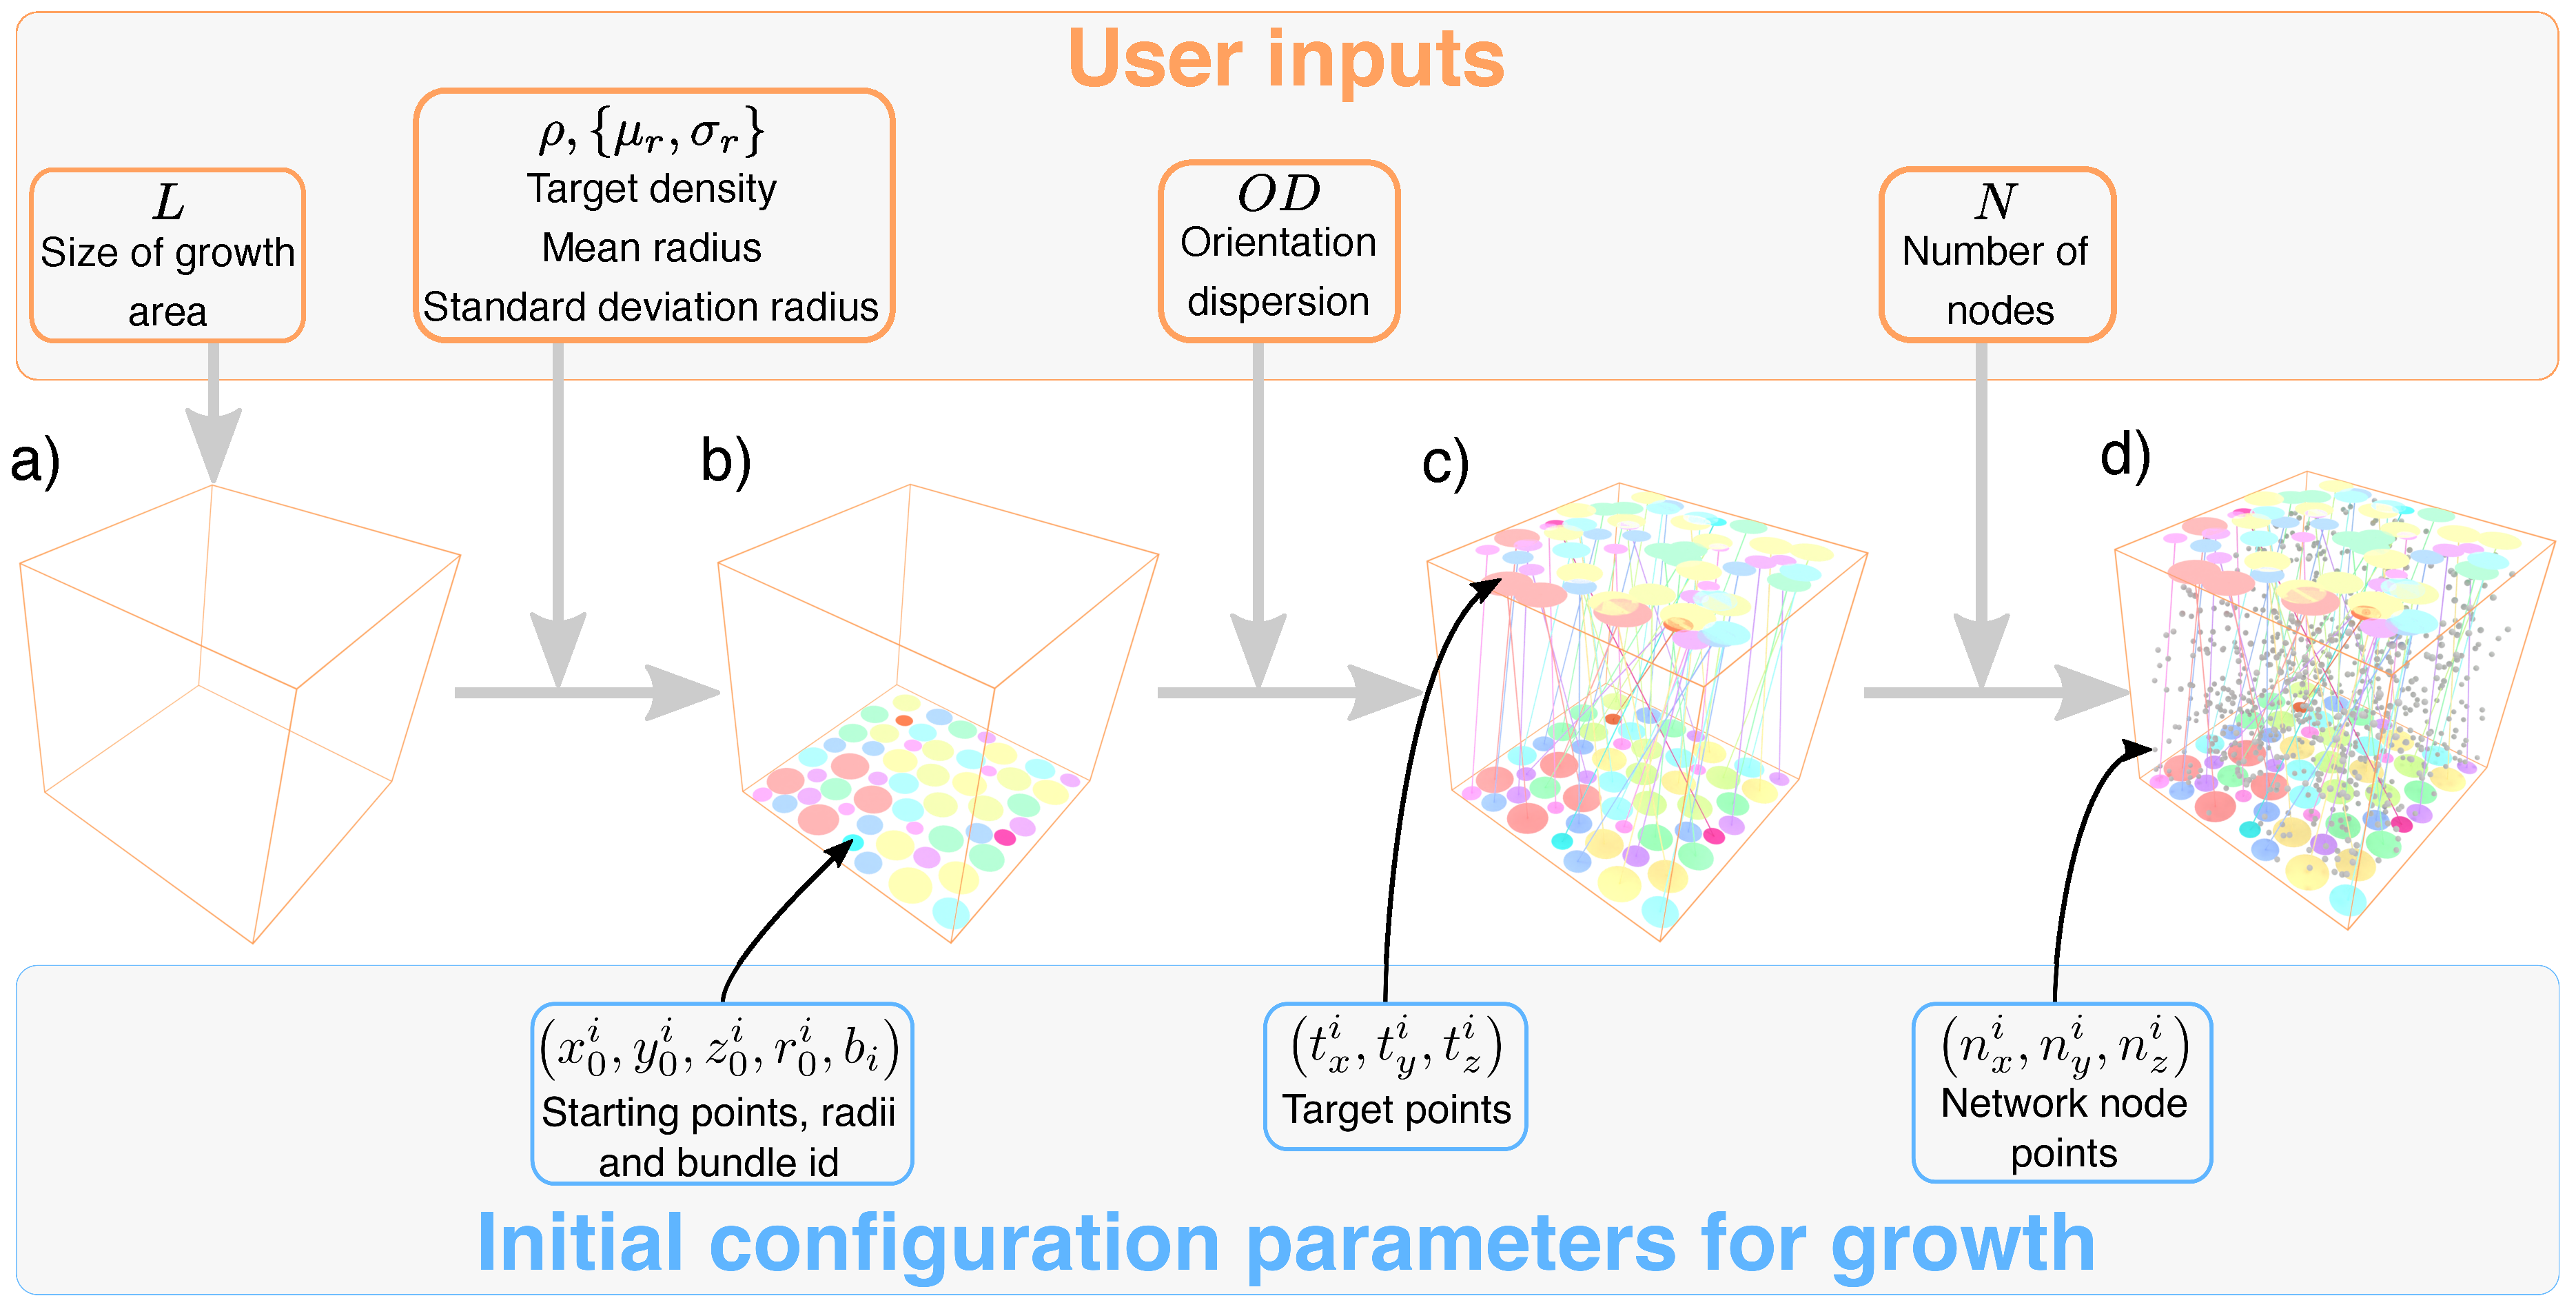
\includegraphics[width=\textwidth]{figures/config/method_inputs_only.eps}
  \caption[Inputs to the \ac{preFiG} algorithm]{Inputs to the \ac{preFiG} algorithm for the single bundle case. $L$ defines the size of the area of that the growth will take place in. The target density and fibre radius distribution govern the generation of starting points for each fibre by packing in 2D. Orientation dispersion parameters govern the generation of target points corresponding to each starting point. $N$ defines the number of nodes to use when generating the network. In the case of multiple bundles, starting and target points are generated for each bundle and then combined into the same space which is filled with nodes for the network. }
  \label{fig:ipmi_inputs}
\end{figure}

\subsection{STEP 1: Initial growth configuration}
\label{sec:ipmi_step1_details}
\textbf{\sffamily STEP 1} is broken down in to three substeps which are outlined in \Cref{fig:ipmi_inputs}:
\begin{description}
  \item [STEP 1.1] Generate fibre starting points for each fibre to grow from (~\Cref{fig:ipmi_inputs}a-b). To generate these starting points \ac{preFiG} packs circles with the desired diameter distribution up to the target density (defined in terms of the desired fibre volume fraction) in 2D, following the approach taken in \cite{Hall2009}.

  \item [STEP 1.2] Generate fibre target points for each point to grow towards (~\Cref{fig:ipmi_inputs}c). To encode the desired orientation distribution, each fibre has a direction drawn from the target distribution which gives a target point for the fibre to grow towards. As a demonstration of the flexibility of the framework, in this work we use the Watson distribution \cite{Mardia2008}.

  \item [STEP 1.3] Generate growth nodes (~\Cref{fig:ipmi_inputs}d). \ac{preFiG} uses a set of pseudorandomly placed points (nodes) to sample the space and encode which regions are occupied by existing fibres. This simplifies collision checking making growth more efficient than a direct collision detection approach involving growing each fibre one small step at a time and checking collisions with existing fibres. This is demonstrated in \Cref{sec:impi_bruteforce}.
\end{description}

\begin{figure}[h!]
  \centering
  \includegraphics[width=\textwidth]{figures/config/method_without_inputs1.eps}
  \caption[Overview of the \ac{preFiG} growth algorithm]{Overview of the basic growth algorithm in \ac{preFiG}. In this example, three fibres are shown with a growth network that only contains relevant nodes for the sake of visualisation.  From the set of nodes, a network is constructed using the Delaunay triangulation. Each fibre then grows from node to node, along any edge connected to the current node. The node moved to will be the node with the lowest cost. Once a fibre segment has grown, the network nodes are updated to store information about which nodes are occupied or near to an existing fibres. This contributes to the cost function for any future fibres, penalising moving to nodes too close to existing fibres.  It is not possible to move to any node now inside a fibre as indicated by the removal of this edges from the network (pairs of blue arrows show where this is happening). The next fibres grow, now avoiding existing fibres until all fibres have finished. See Supplementary Video 1 for an animation of this algorithm. }
  \label{fig:ipmi_config_algorithm}
\end{figure}

\subsection{STEP 2: Fibre growth}
\label{sec:ipmi_step2_growth}
\textbf{\sffamily STEP 2}, the main growth algorithm, is broken down into a series of substeps which are outlined in \Cref{fig:ipmi_config_algorithm}:
\begin{description}
  \item [STEP 2.1] Create growth network (~\Cref{fig:ipmi_config_algorithm}a\&b). In order to encode which nodes a fibre can move to from any other node, the growth nodes are connected using the Delaunay triangulation.

  \item [STEP 2.2] Grow one fibre step (~\Cref{fig:ipmi_config_algorithm}c-e). Fibres grow one-by-one in a random order along this network towards their target points while avoiding existing fibres.

    During growth, a fibre must choose in which direction it should grow. This direction is chosen in \ac{preFiG} by following a cost function which encourages fibres to grow towards their target points (~\Cref{fig:ipmi_config_algorithm}d).
From a starting node, $s$, the candidate nodes, $c$, that the fibre can move to are any nodes that share an edge with $s$. In addition to its position, each network node stores the maximum fibre diameter, $d_c$, that can be sustained at that node without intersecting another fibre (described further in \textbf{\sffamily STEP 2.3}). The fibre will move to a candidate node according to a cost function consisting of two terms; $l_t$, which penalises taking very large steps or moving away from the target point, $t$, and $l_d$, which penalises moving to a position where $d_c$ is low meaning that the fibre will have to shrink. The cost function for a fibre at a position, $s$, to move to a candidate node, $c$, given a target point, $t$, is
\begin{align}
  l &= l_t+fl_d  \,,\label{eq:ipmi_original_cost}\\
      \mathrm{where}\nonumber\\
  l_t &=  \frac{1}{2} \cdot \frac{\|s-c\|}{1+ \|s-c\|} \cdot \left(1- \frac{\left(\left(c-s\right) \cdot \left(t-s\right)\right)}{\|c-s\|\|t-s\|}\right)\,, \label{eq:ipmi_original_lt}\\
  l_d &=\mathrm{max}\left(0, \frac{1}{d_0} \left(d_0 - d_c \right)\right) \,. \label{eq:ipmi_original_ld}
\end{align}
Here, $d_0$ is the target diameter of the fibre and $f$ is a weighting factor between the two terms. In this work, $f$ is fixed to 0.2 to more strongly weight growth towards the target.

The next node for a fibre will be the candidate node which has the lowest cost according to Equation (1). This method of finding a path through the triangulation by choosing the lowest cost node at each position amounts to a greedy best-first pathfinding approach with a heuristic given by Equation (1).

  \item [STEP 2.3] Update the network (~\Cref{fig:ipmi_config_algorithm}f). The growth network is updated in order to store the information about the space this fibre is occupying so that future fibres can avoid it. The way that this is done is to simply store the minimum distance from each node in the network to any existing fibre.

With the next node chosen, the value of $d_c$ needs to be updated for other nearby nodes.
All nodes have $d_c$ set to the Euclidean distance between the node and the surface of the new section of fibre if that distance is less than the current value of $d_c$. This is illustrated in \Cref{fig:ipmi_config_algorithm}d.

Any nodes which now lie within the fibre have $d_c$ set to zero.
Nodes with $d_c = 0$ are disallowed from future steps, meaning that once a fibre has grown, no future fibres can connect to any nodes within the fibre.
This, in addition to shrinking the radius of future fibres according to $d_c$ at each node means that the fibres grow in an almost completely  non-intersecting manner.
Since the value of $d_c$ is set based on fibre-to-point distances, there can be cases in which the fibres would intersect when the closest point between two fibre sections is not at one of the fibre nodes.
In order to account for this, a meshing process developed which can deform fibres around one another. This is described in \Cref{sec:ipmi_step3_meshing}.

  \item [STEP 2.4] Repeat steps 2.2 and 2.3 until fibre reaches target (\Cref{fig:ipmi_config_algorithm}g). By default in \ac{preFiG}, each fibre will grow completely before the next one starts, meaning that step 5 only needs to be performed once the fibre has finished growing. If fibres are allowed to grow concurrently, step 5 must be performed after each growth step.

  \item [STEP 2.5] Repeat steps 2.2-2.4 for remaining fibres (\Cref{fig:ipmi_config_algorithm}h-i). As noted in \Cref{fig:ipmi_config_algorithm} (e-h), as the network is updated, more and more nodes become inaccessible making the network sparser. This means that some fibres may reach a point from which they cannot grow any further and will become stuck. Currently, these fibres are simply removed from the final phantom, meaning the final phantom may have a lower density than the target density.
\end{description}



\subsection{STEP 3: Meshing}
\label{sec:ipmi_step3_meshing}

\begin{figure}
  \centering
  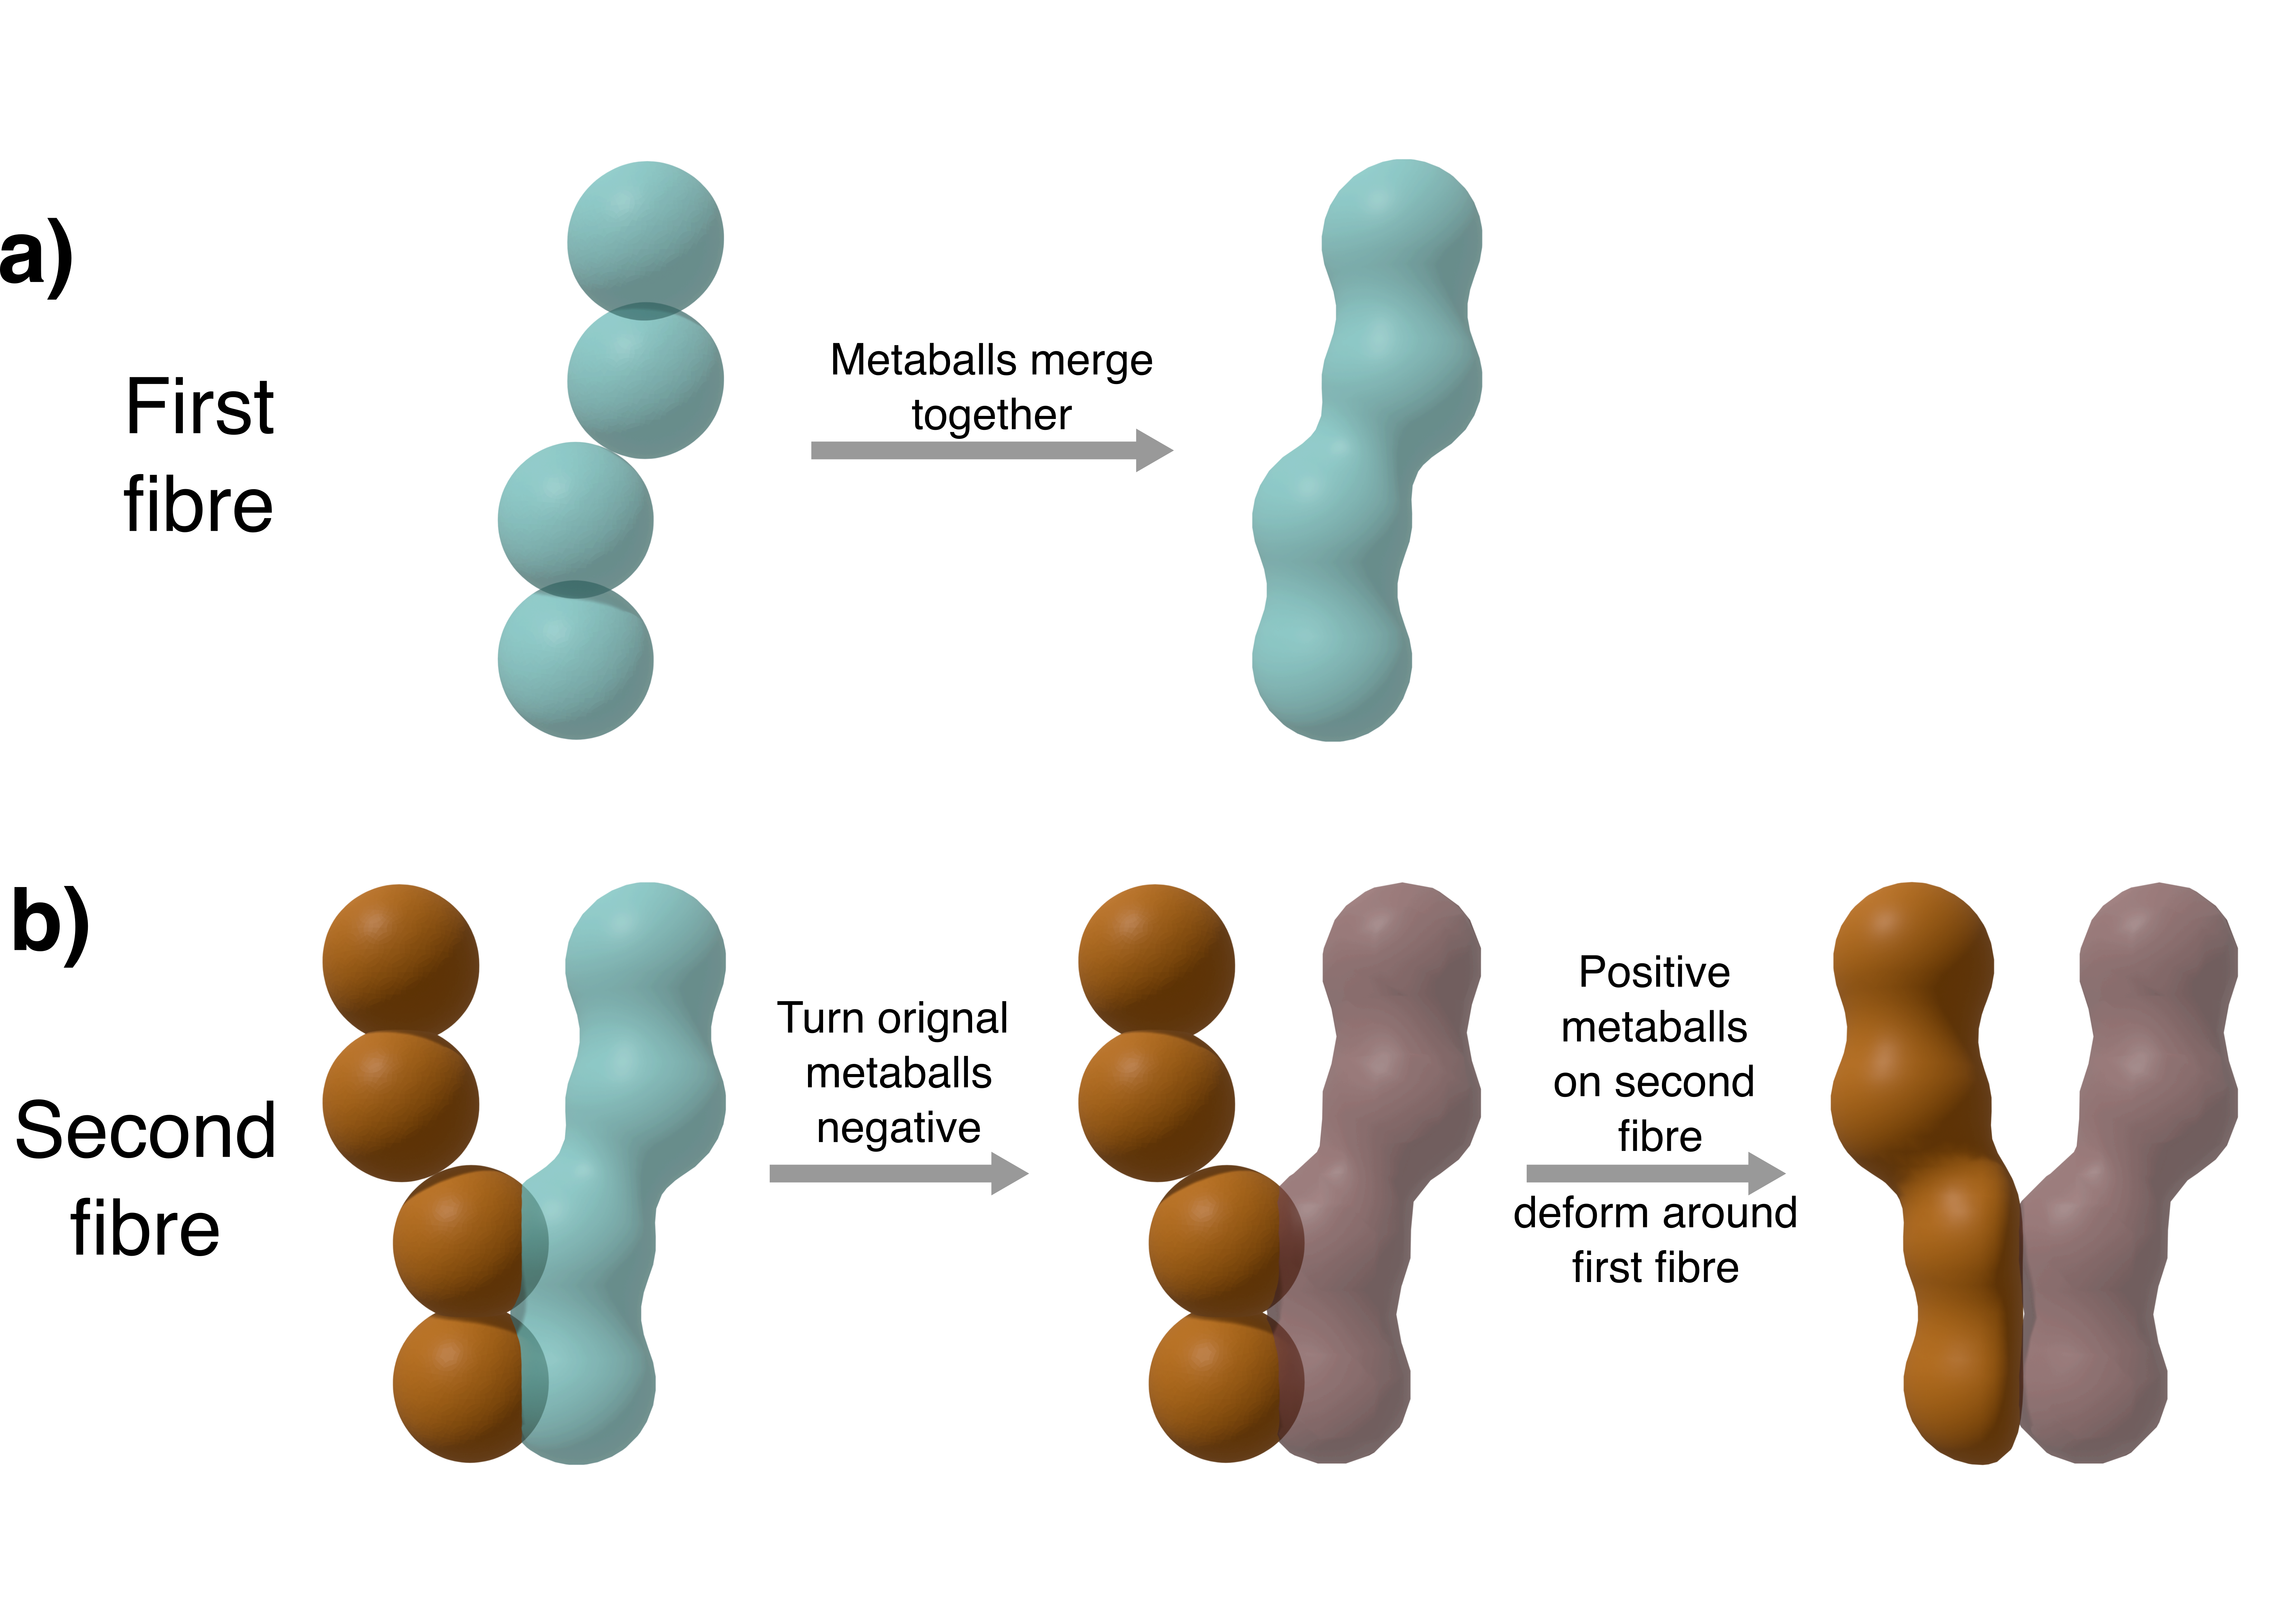
\includegraphics[width=0.8\textwidth]{figures/config/METABALL_fig.png}
  \caption[\ac{preFiG} meshing procedure]{Demonstration of the meshing procedure in \ac{preFiG}. The first fibre is created using metaballs to create a smooth surface. The second, and following fibres will be created using negative metaballs for any fibres that intersect in order to deform around them. Note that in practice, more spheres will be much more closely placed along the skeleton to create a smoother surface}
  \label{fig:ipmi_meshing}
\end{figure}

Finally, Step 3, the meshing procedure is described in more detail below:
\begin{description}
  \item [STEP 3] Generate 3D fibre meshes. After the growth process, each fibre will be represented by a series of connected 3D points and corresponding diameters at each point, stored in the Stockley-Wheal-Cole (SWC) format \cite{Stockley1993}. In order to simulate diffusion MRI signals, these fibre skeleta need to be turned into 3D meshes. \ac{preFiG} uses a meshing procedure designed to eliminate overlap between fibres, using Blender (\url{https://blender.org}), building upon on the SWC mesher addon (\url{https://github.com/mcellteam/swc_mesher}).

\ac{preFiG} meshes are constructed using Blender metaballs, an implicit surface representation which is the isosurface of a function; typically a function analogous to the electric potential from a point charge. When two metaballs come close to one another, the fields combine and the surfaces will merge to form a smooth surface. By placing a series of metaballs along the skeleton of each fibre, a smooth surface is formed for each fibre one-by-one as shown in \Cref{fig:ipmi_meshing}a. Supplementary Figure 1 demonstrates that the \ac{preFiG} meshing procedure does not impact the diffusion dynamics compared to a straight cylinder.

When fibres are densely packed, the surfaces from neighbouring fibres may overlap. To account for this, a meshing procedure was developed in which fibres can deform around nearby fibres to avoid overlap. The metaball surface for one fibre is created as described above. This surface is then turned into a triangulated mesh, however the metaballs are retained. The metaball potential is then turned negative, meaning that rather than merging with any future nearby metaball surfaces, it will repel them, as shown in \Cref{fig:ipmi_meshing}b. This means that subsequent fibres which are meshed very close to, or overlapping with, existing fibres will deform organically to resolve the intersection, thus creating a series of completely non-intersecting fibre meshes which can be used by the dMRI simulator.

\end{description}

% \subsection{Input to the algorithm}
% \label{sec:input}
% The morphology of the final substrate will depend on the inputs to the algorithm which can be split into two general categories: parameters defining the fibre population(s), and parameters defining the space in which fibres grow.

% Fibre parameters include the desired orientation dispersion (OD), packing density ($\rho$) and diameter distribution ($P(d_0)$).
% These three parameters determine the initial settings for each individual fibre.
% Each fibre is defined by a starting point and a target point towards which it will grow as well as an initial fibre diameter, $d_0$.
% These parameters for each fibre are determined from OD, $\rho$ and $P(d_0)$ by packing circles with the diameters drawn from $P(d_0)$ up to a density of $\rho$ in 2 dimensions. Orientation dispersion is introduced by moving the target points of fibres relative to the starting points. %For instance, planar dispersion can be introduced by splitting the substrate into planes and rotating these relative to one another.

% Alternatively, if the user wishes, the starting point, target point and diameter for each fibre can be directly input, rather than allowing \ac{preFiG} to generate them, in order to specify particular fibre configurations such as crossing fibre bundles or fanning fibres.

% Each fibre is allowed to shrink its diameter if it is necessary to fit into spaces close to other fibres.
% The maximum amount of shrinkage permitted is a controllable parameter, specified as a percentage of the initial fibre diameter.

% Due to the stochastic nature of the algorithm, the final substrate is not guaranteed to have the exact morphological properties as input in the priors, however these inputs give the target morphology that \ac{preFiG} will attempt to produce.


% %Parameters defining the space in which the fibres grow are used to define a discretisation of the space which is necessary to make the algorithm run in a practically feasible time.
% %Ideally, the space in which the fibres can grow is a continuous space, so there are an infinite number of positions a fibre can occupy. Practically, this is intractable, so in this algorithm the space is discretised into a set of points which define nodes that the fibres can occupy.

% Parameters defining the space in which the fibres grow are used to define a discretisation of the space into a set of node points that the fibres can occupy. Ideally, the space in which the fibres can grow is a continuous space, so there are an infinite number of positions a fibre can occupy, however this is impractical, so in this algorithm the space is discretised into a finite set of nodes.

% Naturally, the choice of the density and arrangement of node points will impact the substrate that is produced. Too few nodes will result in fibres that have very long, straight segments and may introduce intersections between fibres. Using more nodes will reduce overlap between fibres at the cost of more memory usage and slower growth of the fibres.
% The arrangement of the nodes will also affect the morphology of the final substrate. For instance, placing nodes on a uniform grid may produce fibres with unnaturally angular paths. If the density of nodes on a uniform grid becomes sufficiently high, these angular bends are insignificant compared to the diameter and the fibres will have more natural shapes. For large substrates, the number of nodes required to satisfy this condition becomes intractably large. For this reason, the nodes used are typically pseudo-randomly distributed to ensure broadly uniform coverage of the space, whilst keeping the number of nodes required lower.
% %randomly distributed in the space between the start and target points, to produce more organic shapes whilst keeping the number of nodes necessary lower.

% \subsection{Creation of the Growth Network}
% \label{sec:creation_of_the_growth_network}
% In order to embed information about the local environment at each node, the first step of the algorithm is generating the paths that fibres can take between the nodes as well as defining a maximum diameter that can be sustained at each node to avoid intersection which will be denoted by $d_i$, for a node, $i$. These paths define a network along which the fibres may grow.

% The paths between nodes are defined by the Delaunay triangulation\cite{Delaunay1934} of the nodes which creates a sparse network in which any node can be reached from any other node.
% This triangulation creates edges between nearby nodes, encoding information about the local connectivity at each node.
% Nodes that become occupied by a fibre will be inaccessible to any future fibres, which is one way in which intersection is minimised between fibres.

% The maximum diameter, $d_i$, at each node encodes information on the amount of space available at each node.
% Where $d_i$ is small, that node is close to an existing fibre, so any subsequent fibre passing through that node will have to shrink its diameter to $d_i$ in order to prevent intersections.
% Allowing fibres to contextually shrink their diameter allows fibres to occupy spaces which would otherwise be unavailable.

% \subsection{Growth of a Fibre}
% \label{sec:growth_of_a_fibre}
% \begin{figure}
% 	\centering
% 	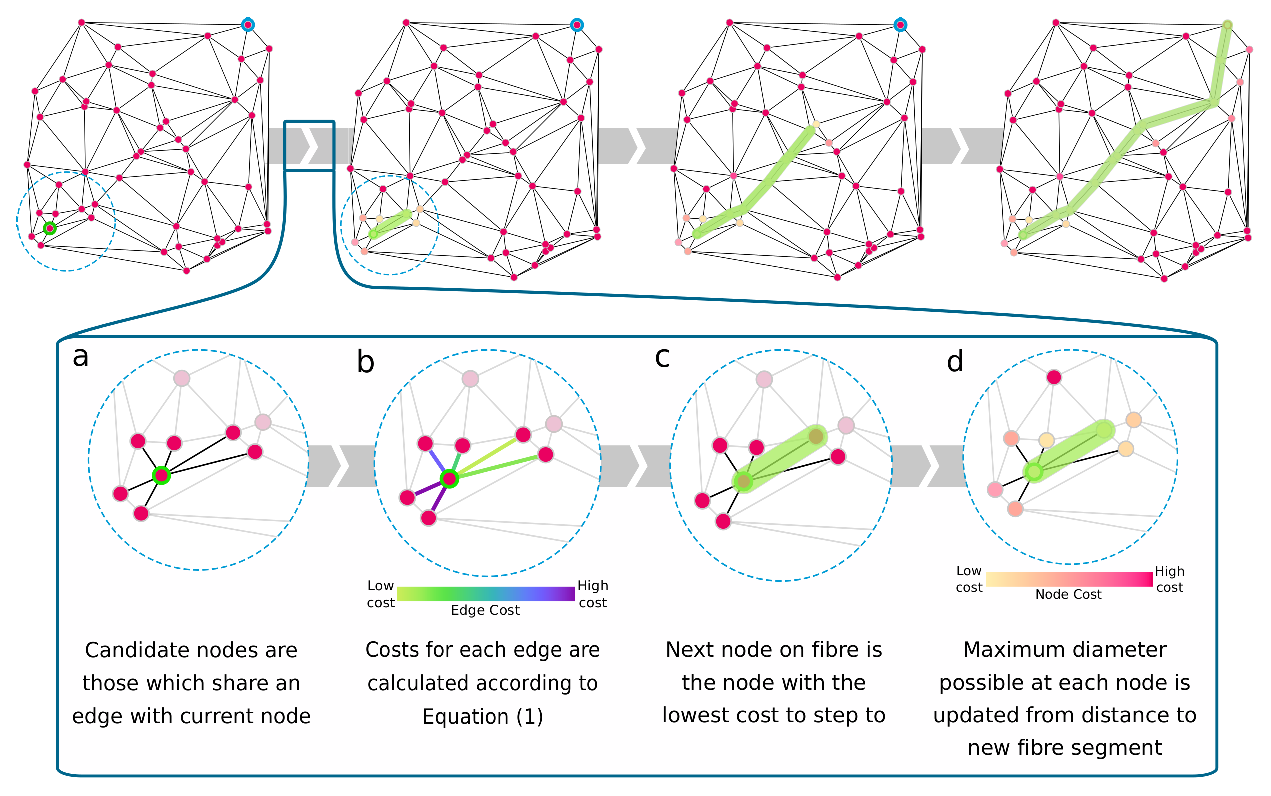
\includegraphics[width = \textwidth]{figures/ipmi_implementation/newMethod_v1.eps}
% 	\caption{\small Schematic overview of the fibre growth algorithm. A fibre grows sequentially, moving from one node to the next, starting from the start point (top left, green node) toward the target (top left, blue node) along the edges defined by the Delaunay triangulation. Inset: The algorithm determining which node a fibre steps to at any given iteration. a) The possible nodes to step to are those which share an edge with the current node. b) From the edges available costs are calculated using \cref{eq:l_t,eq:l_D}. c) The fibre will grow along the edge with the lowest cost. d) From this new segment, the maximum diameter sustainable at a given node is calculated, giving each node a cost based on the maximum sustainable diameter. This cost will then be used in the calculation of edge weights (b) for future fibres. Note that although this figure illustrates the algorithm in 2D, in practice the algorithm grows fibres in 3D.}
% 	\label{fig:method}
% \end{figure}
% Each individual  fibre grows by moving the head of the fibre from node to node according to a cost function which attempts to ensure that the fibre moves towards its target whilst avoiding intersection.
% The main steps in the growth of a single fibre are shown in \Cref{fig:method}.

% The first step in the growth of a fibre is determining which nodes are the possible next nodes the fibre can step to, referred to as candidate nodes.
% From a given starting node, $s$, the candidate nodes are any of the nodes which share an edge with $s$.

% The choice of which candidate node a fibre steps to from the current node is determined by a cost function.
% The cost function consists of two terms, one which penalises moving away from the target point, $t$, and one which penalises moving to a position where $d_i$ is low, meaning the fibre diameter would have to shrink. The cost function for a fibre at a position, $s$, to move to an candidate node, $c$, given a target point, $t$, is $l = l_t + fl_d$,
% % \begin{equation}
% % l = l_t + f l_d\,,
% % \label{eq:costfunction}
% % \end{equation}
% where
% \begin{align}
% l_t &= \frac{1}{2} \cdot \frac{\|s - c\|}{1 + \|s - c\|} \cdot \left(1 - \frac{(c -s)\cdot(t - s)}{\|c-s\|\|t-s\|}\right)\,,\label{eq:l_t}\\
% l_d &= \max\left(0,\, \frac{1}{d_{0}} (d_0 - d_i)\right)\,,\label{eq:l_D}
% \end{align}
% $d_0$ is the desired radius of the fibre and $f$ is a weighting factor between the two terms. In this work, $f$ is fixed to 0.2 to more strongly weight growth toward the target.

% \Cref{eq:l_t} is the term penalising moving away from the target. The dot product between the vector to the candidate and the vector to the target ensures that the minimum cost occurs when the candidate is directly aligned with the target.
% \Cref{eq:l_D} is the term penalising moving to a position where the radius of the fibre must shrink.
% For radii lower than the desired radius of the fibre, $d_0$, \Cref{eq:l_D} grows linearly with distance from $d_0$.
% For radii greater than or equal to $d_0$, \Cref{eq:l_D} is zero, meaning that regions of empty space are equally weighted.

% The next node for a fibre will be the candidate node which has the lowest cost according to \Cref{eq:l_t,eq:l_D}.
% This method of finding a path through the triangulation by choosing the lowest cost node at each position amounts to a greedy best-first pathfinding approach with a heuristic given by \Cref{eq:l_t,eq:l_D}.

% With the next node chosen, the value of $d_i$ needs to be updated for other nearby nodes.
% All nodes have $d_i$ set to the Euclidean distance between the node and the surface of the new section of fibre if that distance is less than the current value of $d_i$. This is illustrated in \Cref{fig:method}d.

% Any nodes which now lie within the fibre have $d_i$ set to zero.
% Nodes with $d_i = 0$ are disallowed from future steps, meaning that once a fibre has grown, no future fibres can connect to any nodes within the fibre.
% This, in addition to shrinking the radius of future fibres according to $d_i$ at each node means that the fibres grow in an almost completely  non-intersecting manner.
% Since the value of $d_i$ is set based on fibre-to-point distances, there can be cases in which the fibres would intersect when the closest point between two fibre sections is not at one of the fibre nodes.
% In order to account for this, a meshing process developed which can deform fibres around one another. This is described in \Cref{sec:creation_of_fibre_meshses}.


% The fibre growth algorithm will output a set of fibres which are defined by a series of nodes and the diameter of the fibre at each node.
% These are written into the Stockley-Wheal-Cole (SWC) format\cite{Stockley1993}, a format commonly used to store cellular morphology information.
% \vspace{-1em}
% \subsection{Creation of Fibre Meshes}
% \label{sec:creation_of_fibre_meshses}
% % \vspace{-0.5em}
% In order to create 3D meshes to be used in dMRI simulations, a meshing process was developed using 3D modelling software Blender (https://blender.org).
% Fibres are meshed one-by-one using the Blender “SWC Mesher” add-on  (https://\\github.com/mcellteam/swc\_mesher) which uses Blender metaballs to make a mesh.

% In Blender, a metaball is an implicit surface defined as the isosurface of a so-called directing structure.
% This directing structure can be seen the source of a static field. For instance a spherical isosurface can be formed with a directing structure which mimics the electric field a point charge.
% When multiple metaballs come close to one another, the fields will combine to form a surface that merges the two spheres together.
% An example of metaball interactions is shown in \Cref{fig:metaballs}.

% By placing metaballs along the skeleton of each fibre, with the path and diameters given from the fibre growth algorithm, a smooth surface is formed for each fibre.
% It is this implicit surface, created using metaballs that the SWC mesher add-on creates.
% This implicit surface can be turned into an explicit surface (i.e. a mesh of vertices and faces) in Blender, which can then be refined by progressively smoothing and reducing the number of faces in the mesh to create a mesh which can be used in dMRI simulations.

% This process can be used to mesh each fibre individually, however issues can arise with intersection of fibres, as mentioned in \Cref{sec:growth_of_a_fibre}.
% In order to account for this, a contextual meshing algorithm was developed.
% The metaball surface for one fibre is created using the SWC Mesher.
% This surface is then turned into a mesh as described above, however the metaballs are retained.
% The metaball potential is then turned negative, meaning that rather than attracting any future nearby metaball surfaces, it will repel them, as shown in \Cref{fig:metaballs}b.
% This means that subsequent fibres which are meshed very close to, or overlapping with existing fibres will deform organically to resolve the intersection, thus creating a series of completely non-intersecting fibre meshes which can be used by the dMRI simulator.

% The deformation introduced by the contextual meshing process has two effects.
% As well as helping to prevent intersection between fibres, the deformation produces fibres with more organic non-circular cross sections, better mimicking realistic mythologies.
% This is vastly different to the majority of previous WM numerical phantoms which model fibres as circular or elliptic cylinders.


% \begin{figure}
%   \centering
%   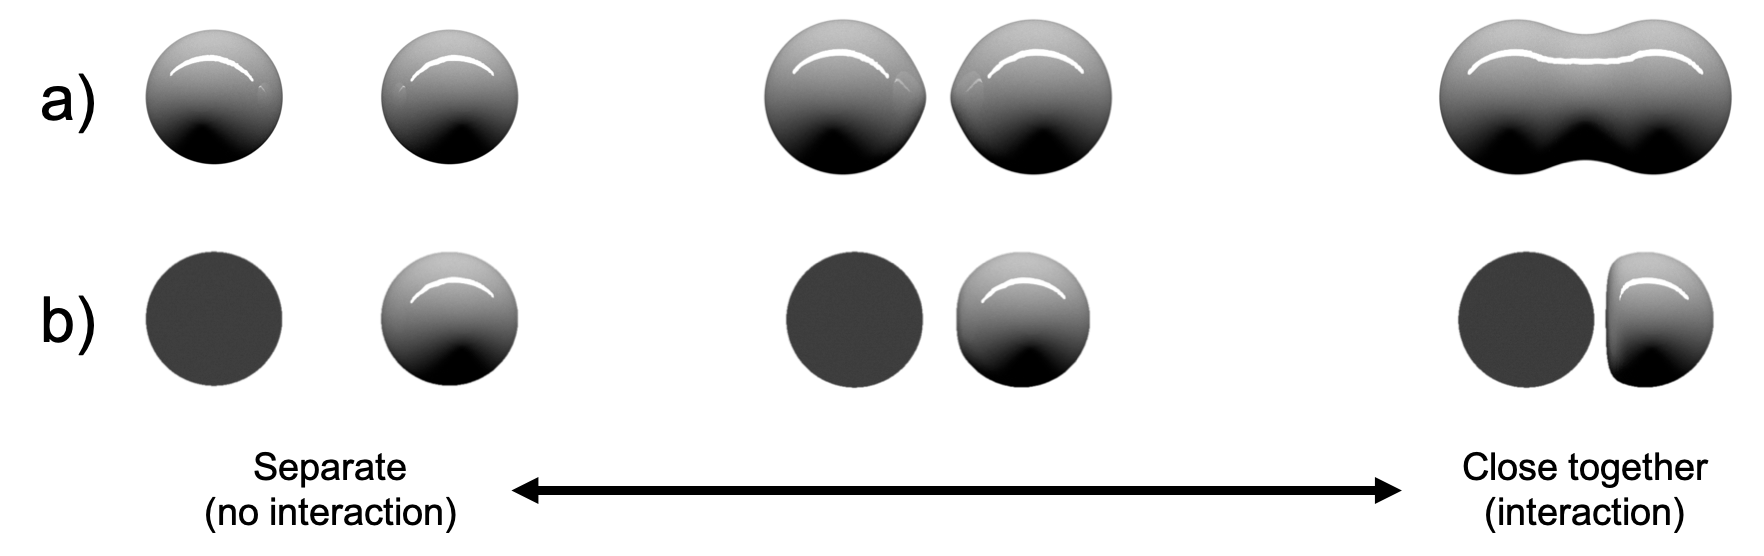
\includegraphics[width=\textwidth]{figures/ipmi_implementation/metaballs.png}
%   \caption{\small Simple example of metaball interactions. a) With two positive metaballs, the fields combine to attract the surfaces together. This is used to join individual segments into a continuous fibre. b) With one negative metaball (indicated by the flat grey circle) the surface of the metaball is repelled from the negative metaball. This is used to deform nearby fibres around one another.}
%   \label{fig:metaballs}
% \end{figure}



\section{Experiments and Results}
\label{sec:impi_experiments_and_results}
\subsection{Effect of Choice of Growth Network}
\label{sec:ipmi_choice_of_network}
\begin{figure}
  \centering
  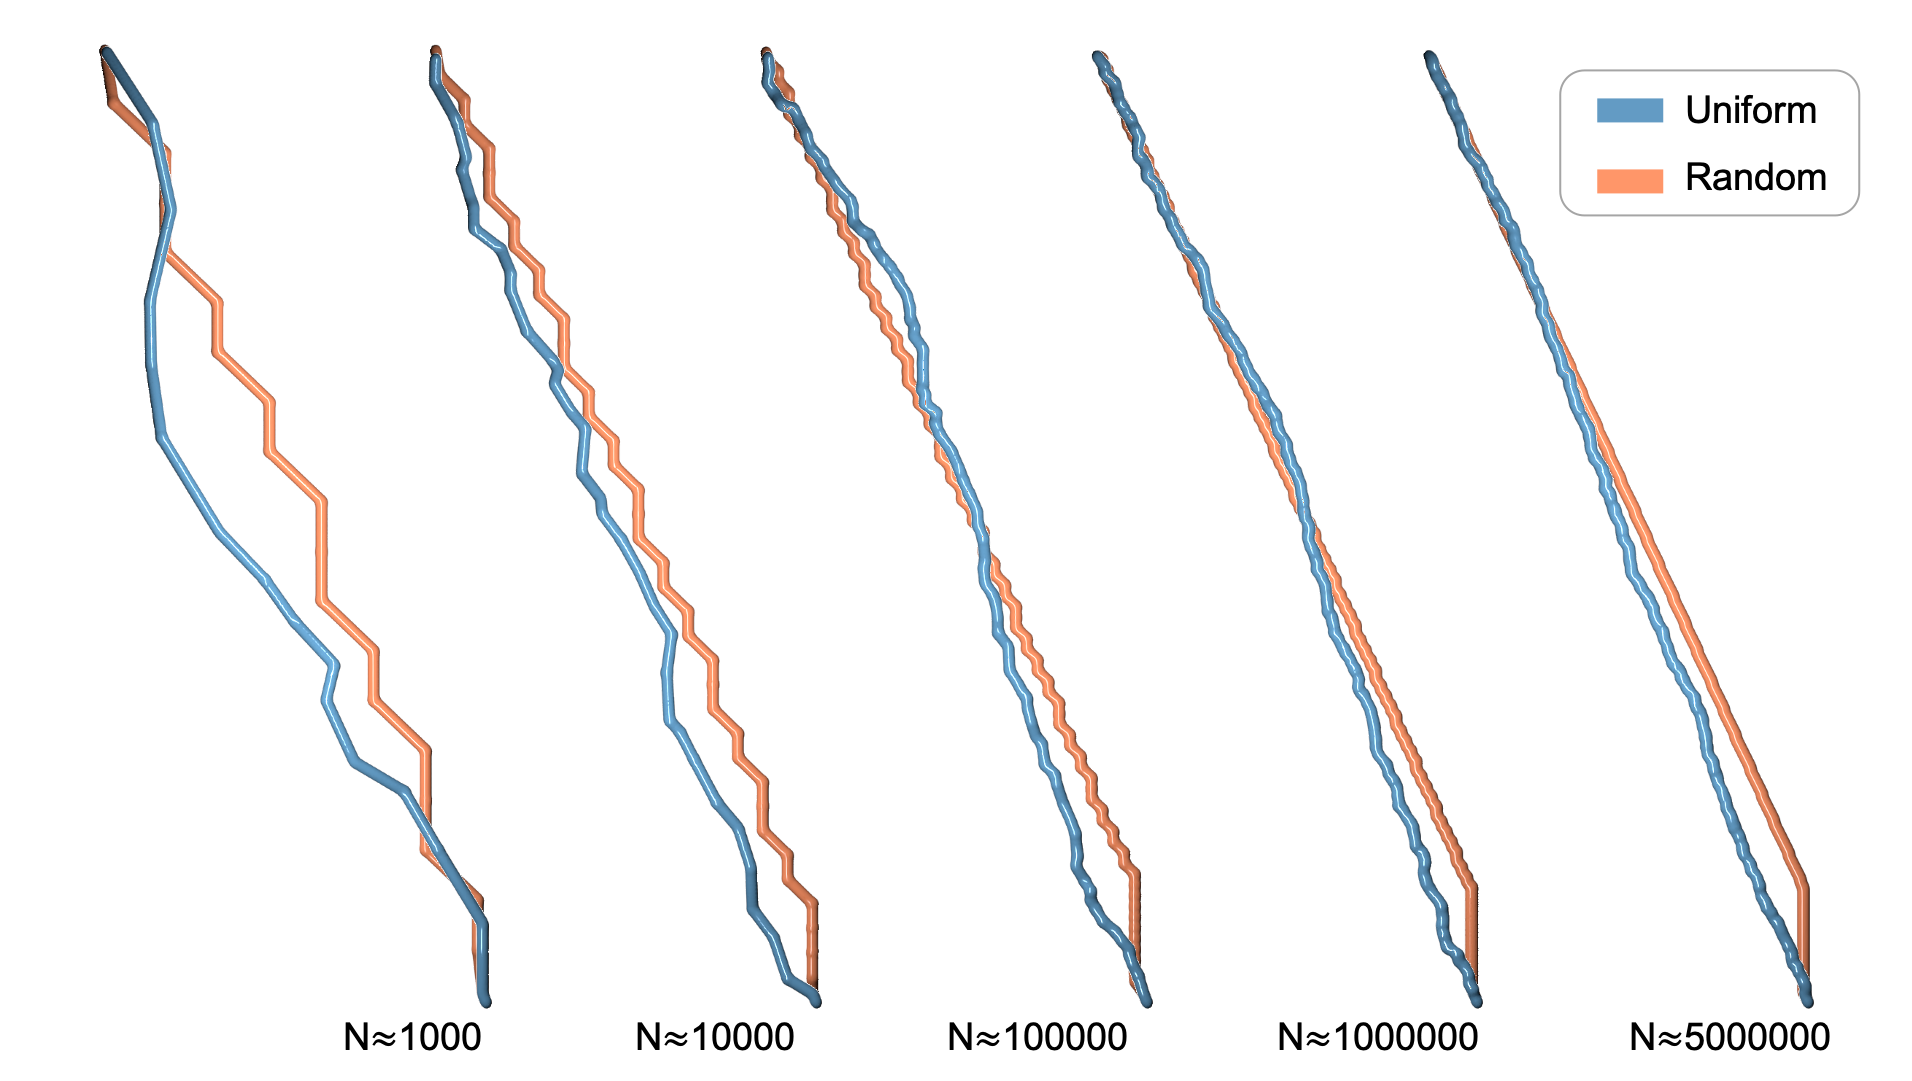
\includegraphics[width=0.9\textwidth]{figures/ipmi_implementation/uniform_vs_rand.png}
  \caption{Fibres generated using uniform grid (orange) and pseudo-random (blue) network nodes for increasing numbers of nodes.}
  \label{fig:ipmi_uniform_vs_rand}
\end{figure}
As mentioned in \Cref{sec:ipmi_step1_details}, the choice of the node points in the network will affect the morphology of the resulting substrate.
In order to investigate this, a qualitative experiment was performed in which a single fibre was grown on a network with either a) nodes on a uniform grid or b) pseudorandom nodes.
In each case, the number of nodes was increased and the resulting fibre investigated.

The fibre was defined by a start point (20, 0, 0) $\mu$m,  target point (0, 0, 50) $\mu$m and diameter 1 $\mu$m.
This configuration was chosen so that the fibre would not have a path that directly followed one of the 90\degree\ or 45\degree\ lines in the uniform grid.
Node points were initialised in either a uniform grid or pseudorandomly within the space [-5, -5, -5] to [25, 5, 55] to ensure coverage of the space in which the fibre would grow.
The number of source points used was $N \approx 1000, 10000, 100000, 1000000, 5000000$.

The resulting fibres can be seen in \Cref{fig:ipmi_uniform_vs_rand}, where orange fibres are grown using the uniform grid and blue fibres using pseudorandom points.
In both cases, as the number of nodes increases, the resulting fibre has more of a smooth, straight path between start and target.
The uniform grid fibres, have a much more angular, structured path due to being forced to grow on the grid, while the pseudorandom fibres more irregular paths, which could be considered more `organic' looking.


\subsection{Demonstration of \ac{preFiG}}
\label{sec:ipmi_demonstration}
To demonstrate the potential of \ac{preFiG}, three substrates at different (dispersion, packing density) conditions were generated: (0\degree, 60\%), (15\degree, 30\%) and (35\degree, 25\%), shown in \Cref{fig:ipmi_substrates_signals}a.
Each substrate is grown using $5 \times 10^6$ pseudo-randomly placed source nodes for the growth network, giving a network with $3.88\times10^7$  edges and a mean distance between any given node and its neighbours of 0.29 $\mu$m.
The packing densities chosen represent the highest densities achievable using \ac{preFiG} for each dispersion condition.


For the 0\degree\ dispersed substrate, initial diameters were drawn from a gamma distribution with mean $d_0 = 2\ \mu$m and standard deviation $\sigma_d = 0.2\ \mu$m. The 15\degree\ and 35\degree\ substrates were generated with $d_0 = 1.2\ \mu$m and $\sigma_d = 0.2\ \mu$m in order to show the flexibility of \ac{preFiG} to generate substrates with different diameter distributions as well as orientation dispersion and packing density. Diameters were limited to be permitted to shrink to 25\% of the original fibre diameter in order to fit into space.

For each substrate, the \acf{PGSE} signal was simulated in Camino\cite{Cook2006} using $5\times 10^5$ diffusing spins and $5\times 10^3$ discrete time steps, uniformly distributed with bulk-diffusivity D$_0$=2 $\mu$m$^2$/ms. To show the range of simulation possibilities available, three different membrane permeabilities ($\kappa$=0, 0.0025, 0.0050 $\mu$m/ms) were also imposed.
The simulated \ac{PGSE} measurement parameters were: $\delta/\Delta=1/40$ ms and 50 b-values from 0 to 9 ms/$\mu$m$^2$ along x-, y- and z-directions.

The corresponding direction-averaged simulated \ac{PGSE} signals at different permeabilities are shown with SNR = $\infty$ in \Cref{fig:ipmi_substrates_signals}b and SNR = 20 in \Cref{fig:ipmi_substrates_signals}c.
The signal decays to a lower value as the dispersion increases and density decreases, as expected.

\begin{figure}[h!]
  \centering
  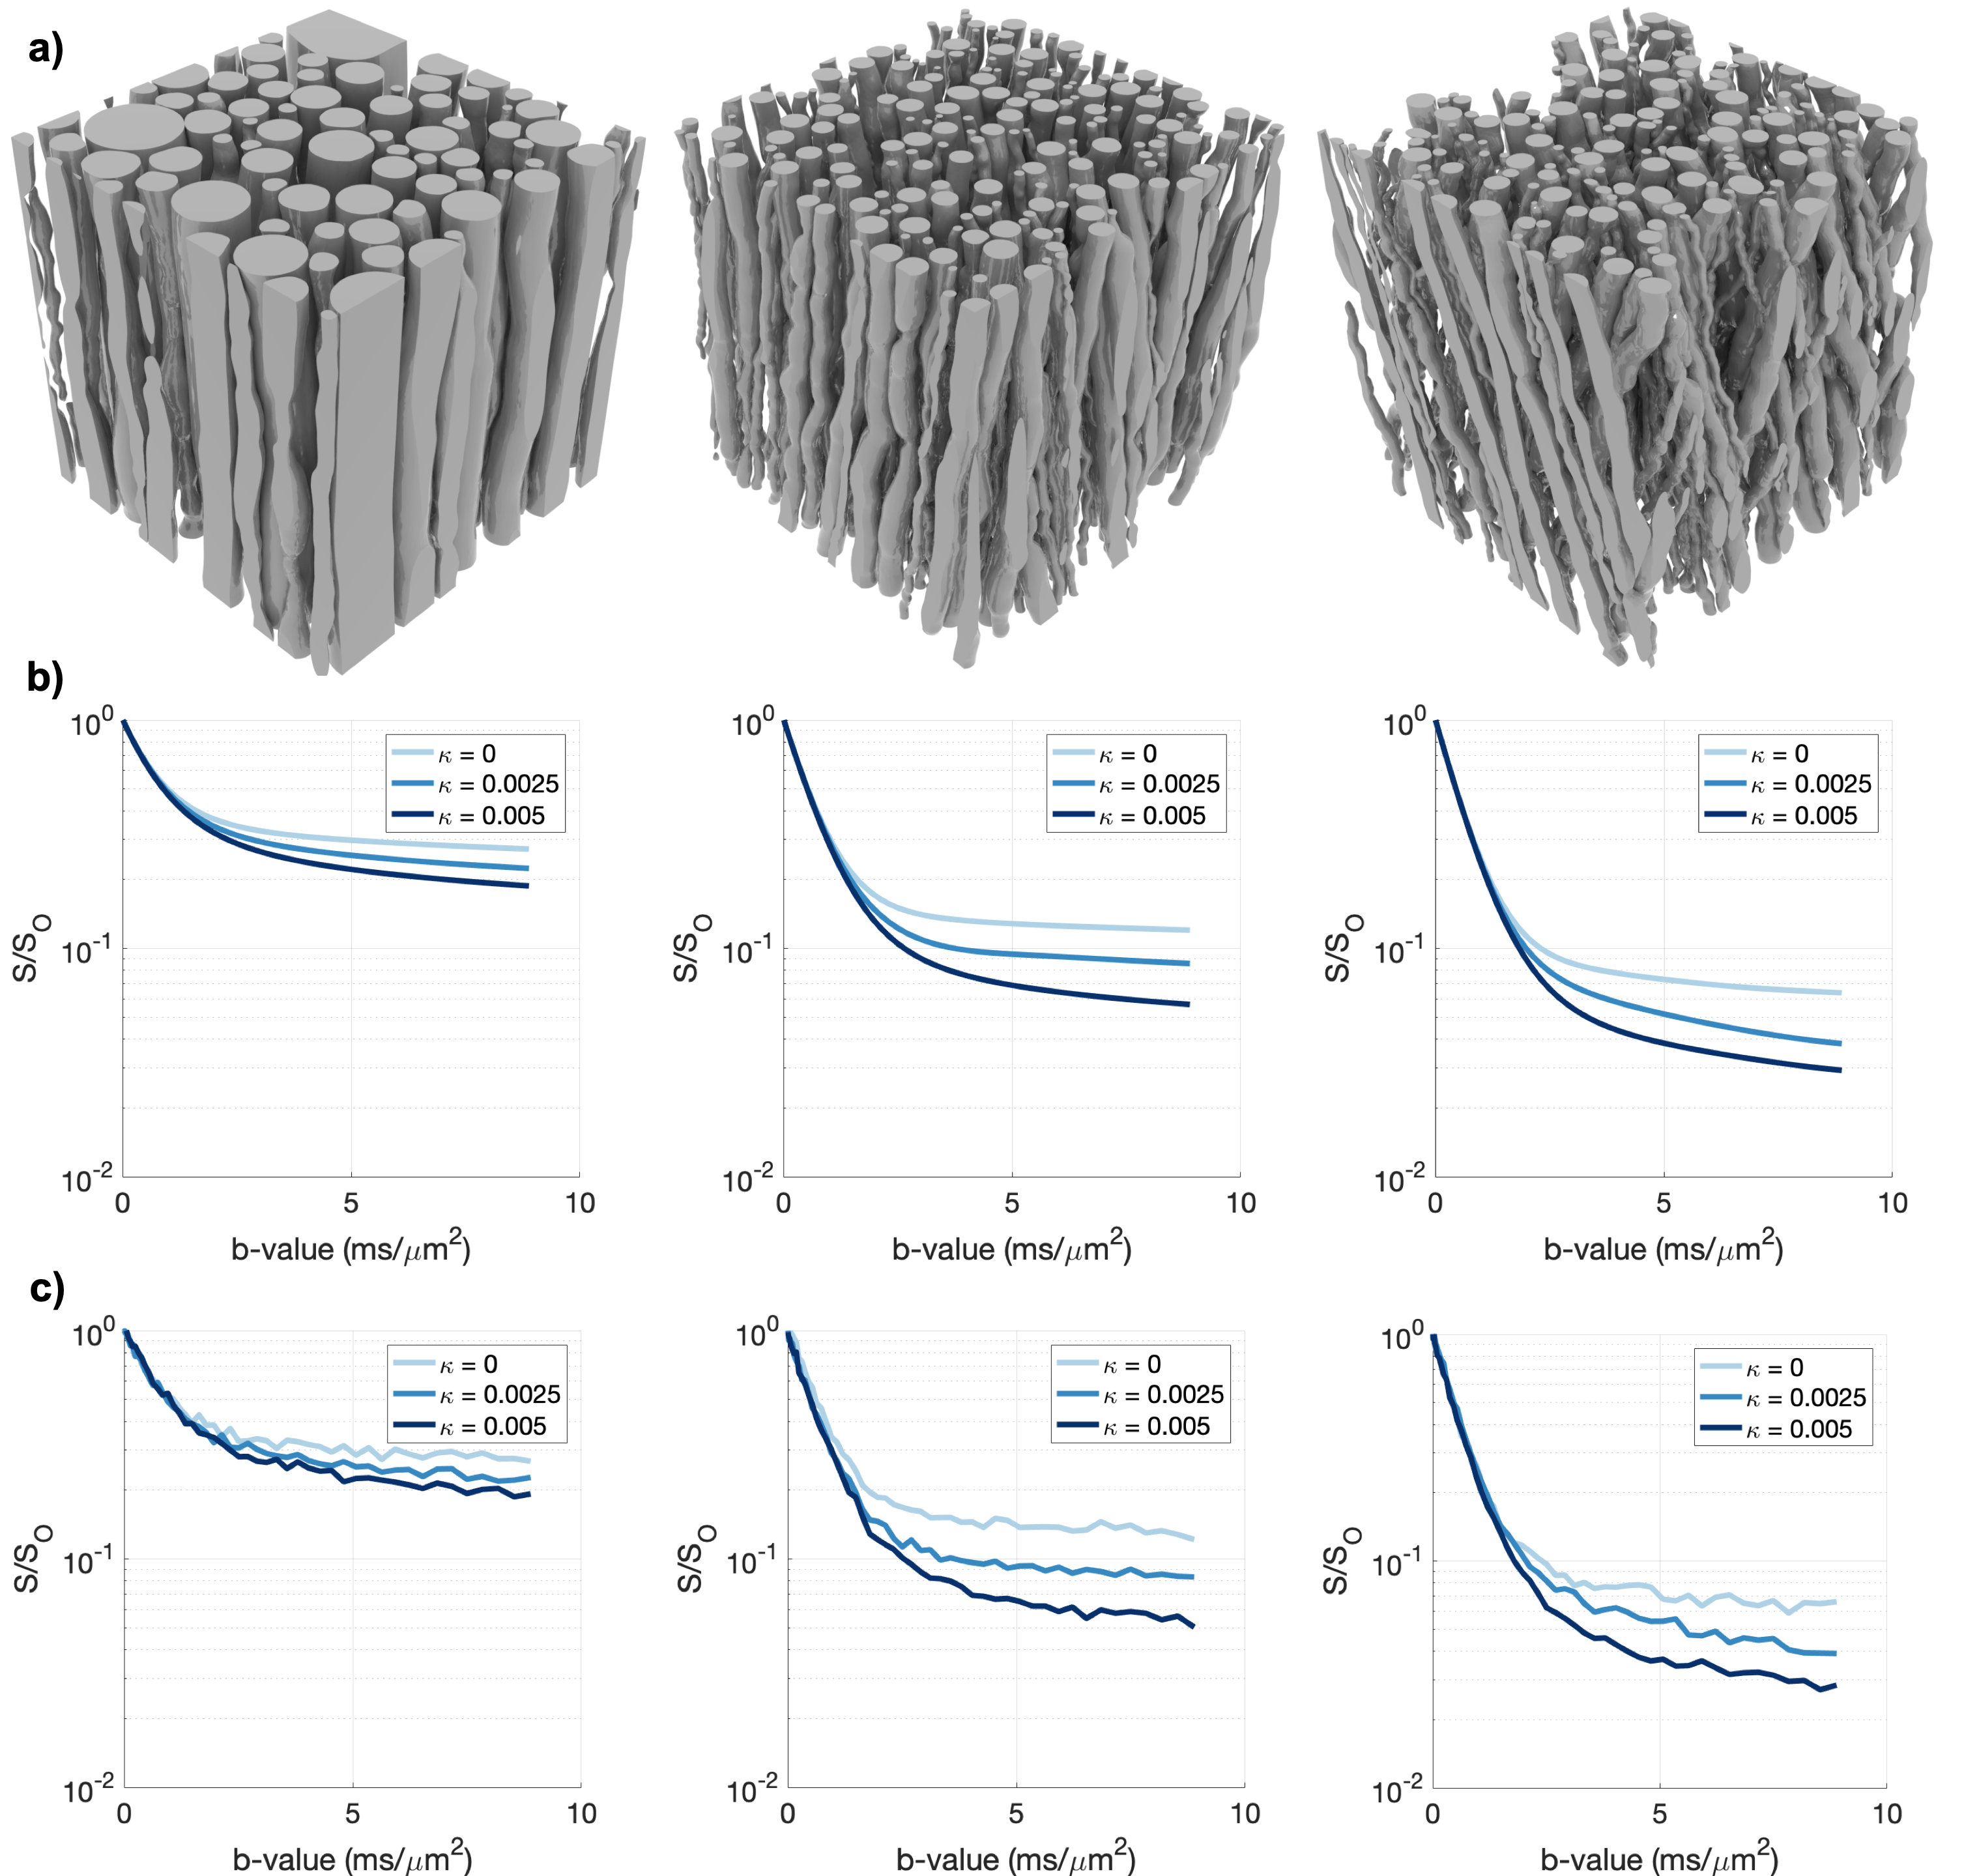
\includegraphics[width=\textwidth]{figures/ipmi_implementation/substrates_and_signals_otherlabels.png}
  \caption[Examples of generate WM numerical phantoms and simulated dMRI signals]{\small a) Example substrates (cut into 30x30x30 $\mu$m$^3$ cube) from the fibre growth algorithm, left to right:  Zero macroscopic dispersion (60\% density), 15\degree\ of macroscopic dispersion (30\% density), 35\degree\ dispersed (25\% density). b) Simulations for each substrate for varying permeabilities with SNR = $\infty$  and c) SNR = 20. Units of $\kappa$ are $\mu$m/ms.}
  \label{fig:ipmi_substrates_signals}
\end{figure}

\subsection{Comparison with Brute-Force Approach}
\label{sec:impi_bruteforce}
\ac{preFiG} was compared against the na\"ive brute-force approach to fibre growth.
The brute-force approach grows fibres one segment at a time and checks for collisions between the new segment and all existing fibres.
Each new segment is chosen from one of 128 candidate directions on a cone aligned with the previous segment, with each direction being weighted according to \Cref{eq:ipmi_original_lt}.
%In the case of collisions between the proposed new section and an existing fibre, each direction is tested in order of the weight of the direction until a non-colliding direction is found, or all directions have been tested and the fibre is stuck.

Substrates were grown with both the brute-force approach and \ac{preFiG} using the same starting and target points and initial diameters.
These initial parameters were determined by packing circles with gamma distributed radii (mean $d_0 = 2\ \mu$m, standard deviation $\sigma = 0.6\ \mu$m) into a 40 $\mu$m x 40 $\mu$m square up to a packing density of 60\%. Target points were set as 40 $\mu$m directly above the starting points to define a substrate with 0\degree\ macroscopic orientation dispersion.
This resulted in a substrate with a total of 54 initial fibres.

The fibre growth algorithm used $1\times 10^6$ randomly distributed points for the Delaunaty triangulation giving a mean distance between points of 0.5 $\mu$m, matching the brute force approach which used a segment length of 0.5 $\mu$m for each new fibre segment.

From these initial parameters, fibres were grown using a subset of $n = 1, 5, 10, 15, 20, 25, 30, 40$ fibres and the growth was timed. Each value of $n$ was timed 5 times with and the mean taken to reduce single-run timing fluctuations.

\begin{figure}[t]
  \centering
  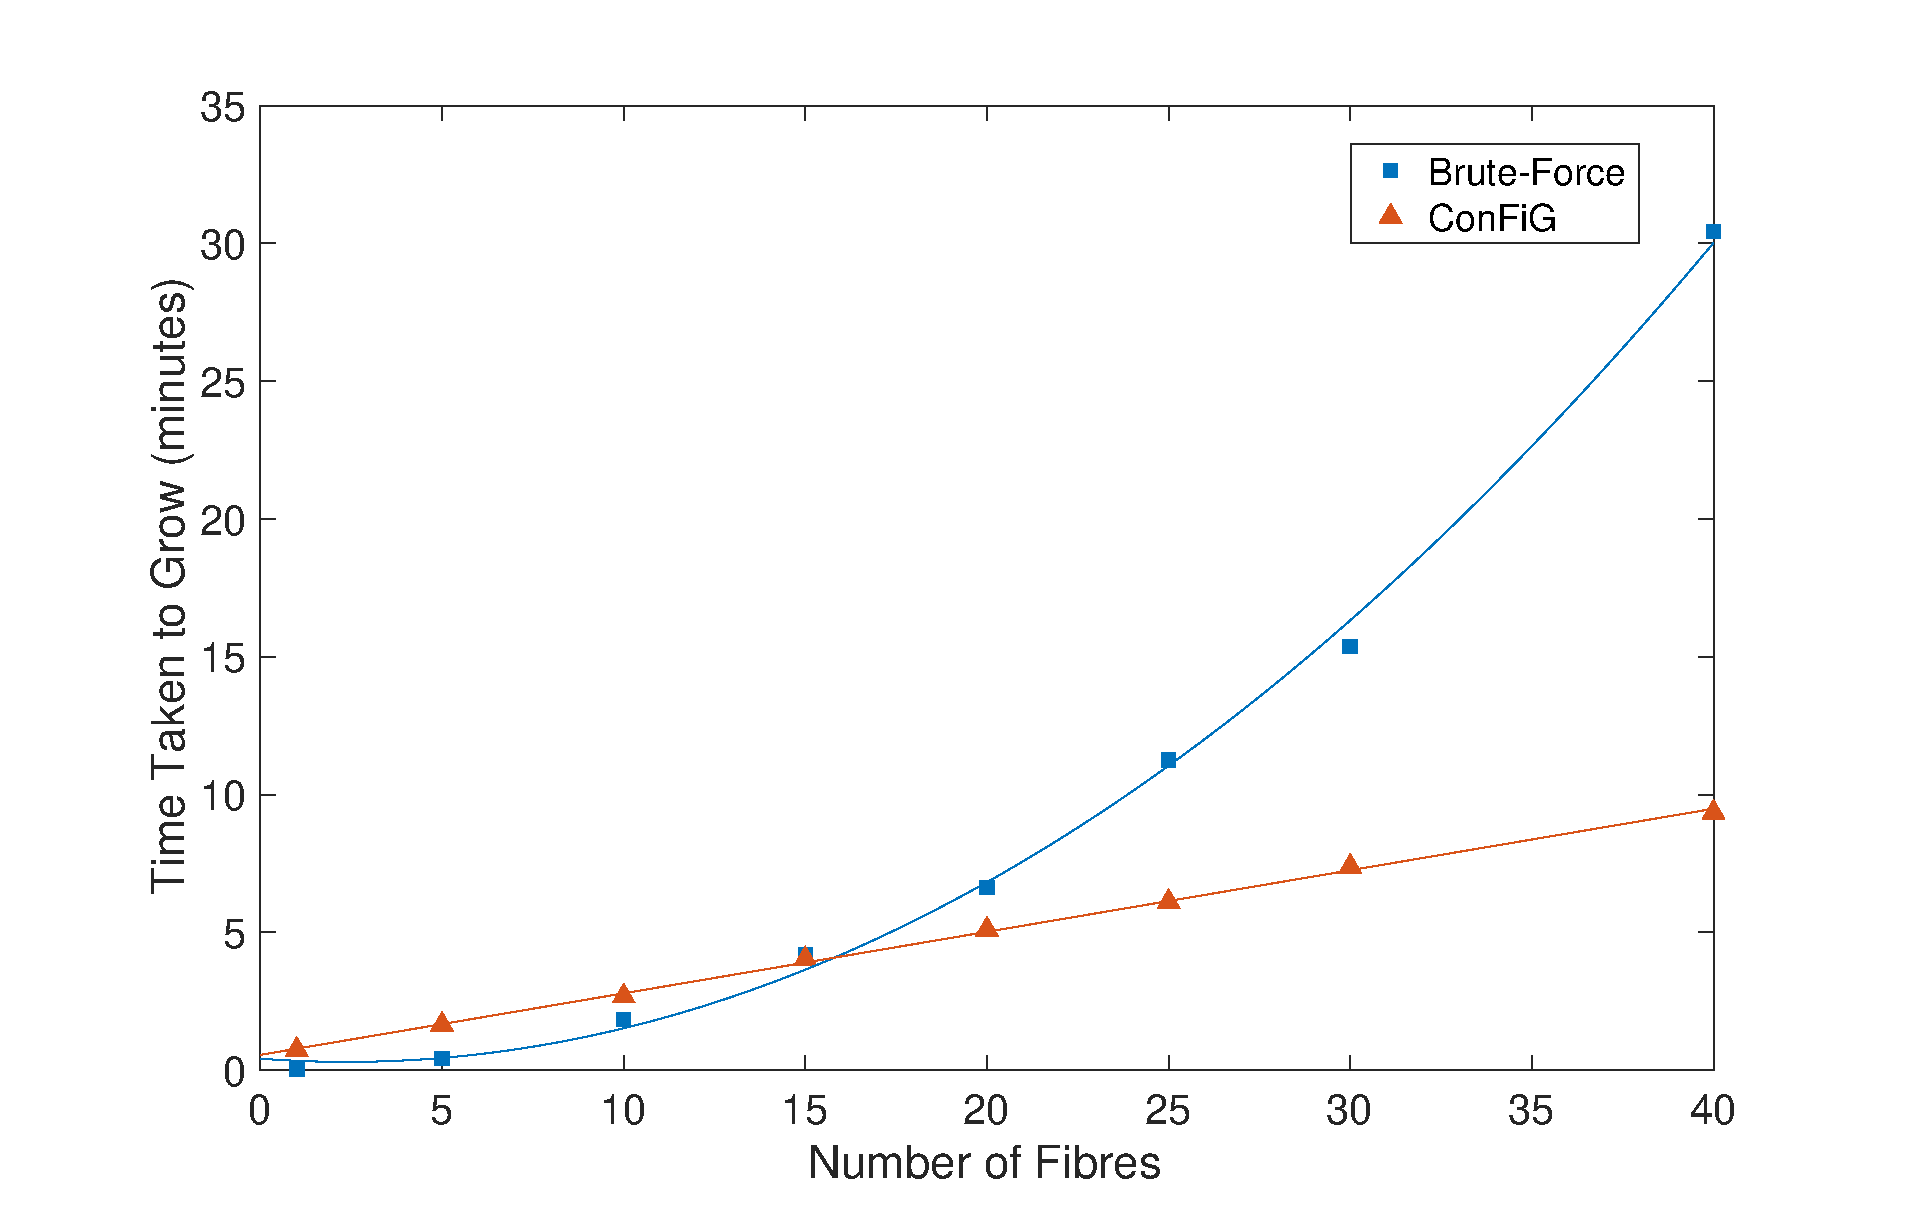
\includegraphics[width=0.8\textwidth]{figures/ipmi_implementation/brute_force_vs_algo_2.eps}
  \caption[Comparison of brute-force growth and proposed fibre growth algorithm]{\small Timing of brute force growth vs.\ the fibre growth algorithm along with a quadratic fit (brute-force) and linear fit (fibre growth algorithm). The fibre growth algorithm is clearly linear in the number of fibres, while brute force growth fits an order $n^2$ well. }
  \label{fig:impi_brute_force}
\end{figure}

\Cref{fig:impi_brute_force} shows the timing results of the brute-force approach versus the fibre growth algorithm.
The fibre growth algorithm  has approximately $\mathcal{O}(n)$ complexity with $n$ being the number of fibres.
Conversely, the brute-force algorithm shows $\mathcal{O}(n^2)$ complexity owing to the fact that every new segment has to check for collisions with all existing fibres.

The fibre growth algorithm has a higher $n=0$ offset which is caused by the overhead in calculating the Delaunay triangulation for the growth network.
This causes the brute-force approach to have better performance at low $n$, while at higher $n$ (approaching the $>100$ fibres needed for a realistic dMRI voxel) the linearity of the fibre growth algorithm gives it much faster performance.



\section{Discussion and Conclusion}
\label{sec:ipmi_discussion}
\ac{preFiG} shifts perspective from previous works attempting to pack together fibres, by trying to mimic natural fibre genesis.
This approach represents a major step towards very high fibre packing, enabling us to reach the highest dispersion at the highest packing density reached so far, to our knowledge. Our (15\degree, 30\%) and (35\degree, 25\%) represent an average \mytilde50\% and \mytilde200\% improvement, respectively, over the best previously reported results of (10\degree, 20\%)\cite{Ginsburger2018}.


The substrates presented in \Cref{fig:ipmi_substrates_signals} are just a few examples of the kinds of substrates that can be produced using our \ac{preFiG} method.
By varying the setup of the morphological controls and start and target points, many different fibre configurations can be produced.
Currently, fibres will attempt to grow in a straight line between the start and target points, meaning that certain configurations such as kissing bundles cannot be represented.
However, the algorithm can in principle be extended to allow for series of target points, allowing the definition of a desired 'path' of a fibre.

Additionally, some input parameter settings cannot be achieved.
For instance, trying to grow a substrate with both very high density and very high dispersion will result in a final substrate that does not reach the density required.
The reason for this could be a combination of limitations of the algorithm in restricting growth to a discrete network and also the fact that some morphological settings are practically infeasible.
This limitation, however, also applies to the fibre packing and  brute force growth approaches.

One weakness of the fibre-growth algorithm is that since the fibre diameters are calculated from a fibre-to-point distance, there can still be some small amount of overlap between fibres.
This is solved using the meshing process in Blender to deform the regions of slight overlap between neighbouring fibres.

To conclude, the proposed \ac{preFiG} approach, using the fully connected growth network, is shown to be more efficient than a `brute-force' growth approach.
The fact that \ac{preFiG} is linear with the number of fibres makes it far more efficient for high numbers of fibres. For instance, a realistic voxel will need hundreds or thousands of fibres which will become impractically slow for the `brute-force' approach, whilst remaining manageable for our algorithm.
This efficiency, along with the high density and orientation dispersion achieved means that \ac{preFiG} represents a promising step forward in the construction of ultra-realistic numerical phantoms of WM.


%%% Local Variables:
%%% mode: latex
%%% TeX-master: "../main"
%%% End:

\chapter{ConFiG: Contextual Fibre Growth}
\label{chap:config}

\chaptertoc{}

\begin{chapterabstract}
  This chapter introduces a series of mechanisms which were added to improve the initial implementation of \ac{ConFiG} described in \Cref{chap:ipmi-implementation} and the biological fibre growth processes which inspire these mechanisms.

  These improvements are tested against the state of the art MEDUSA algorithm and simulated \ac{dMRI} signals compared to real \ac{dMRI} signals from the \acl{WM} of a healthy subject.
\end{chapterabstract}

\section{Introduction}
\label{sec:config_introduction}
Numerical phantoms play a valuable role in the development and validation of many \ac{MRI} techniques.
In particular, numerical phantoms are often used when developing \ac{dMRI} microstructure imaging techniques where simulations of the \ac{dMRI} signal in phantoms with known microstructural properties are used in lieu of an in vivo ground truth measure of microstructure \cite{Alexander2017}.
While recently numerical phantoms have proven useful for validating microstructure imaging of grey matter \cite{Palombo2020}, they have more commonly been used for validating \ac{WM} microstructure, with many studies comparing parameter estimates from fitting their models to the known ground truth from the phantoms e.g. \cite{Li2019,Jelescu2017,Scherrer2016,Tariq2016,Daducci2015,Nilsson2017,Xu2014,Zhang2012,Nilsson2010}.
Some recent works directly estimate microstructural features using fingerprinting techniques and machine learning to match simulated signals and the corresponding ground truth microstructure of the numerical phantom to the measured signal\cite{Hill2019,Palombo2018a,Rensonnet2018,Nedjati-Gilani2017}.
As well as affecting the \ac{dMRI} signal, microstructural features also influence other MR techniques such as susceptibility-weighted imaging \cite{Li2012,Lee2010}.
For instance, Xu et al. \cite{Xu2018} recently used simulations to show that using realistic axonal models rather than simple circular cylinders affects the MR signal.
Therefore, it is important to the \ac{MRI} community to generate realistic \ac{WM} numerical phantoms which accurately capture microstructural features in order to get realistic simulated signal.

Typically, however, there is a mismatch between the complexity of true brain tissue microstructure and the models used in simulation, with simulations simplifying the microstructure.
On one hand, \emph{ex vivo} \ac{EM} studies have revealed the high complexity of real axonal morphology \cite{Abdollahzadeh2019,Lee2019b,Salo2018}.
Reconstructions of axons from these studies show that real \ac{WM} contains axons with complex morphologies on an individual axon basis such as undulation, beading and non-circular cross sections, as well as non-trivial configurations including orientation dispersion and crossing bundles.
On the other hand, the models used in simulation studies often represent axons in \ac{WM} using simplistic geometrical representations such as parallel cylinders with uniform \cite{Fieremans2010,Nilsson2010,Nilsson2009,Ford1997} or polydisperse \cite{Alexander2010,Hall2009} radii.
Some studies investigate the effect of differing configurations of fibres such as simple crossing \cite{Rensonnet2017,Zhang2011a} and orientation-dispersed \cite{Tariq2016,Zhang2012,Zhang2011} fibre bundles.
A few groups generate \ac{WM} numerical phantoms with complex fibre configurations for the application to  tractography \cite{Close2009,Neher2014}; however realistic microstructural morphology is not the focus of these approaches.

Other studies introduce more microstructural complexity into the numerical phantoms, typically only considering one mode of morphological variation at a time; some examples of this include harmonic beading \cite{Budde2010,Landman2010}, spines \cite{Palombo2018}, undulation \cite{Brabec2019,Nilsson2012} and myelination \cite{Brusini2019}.


Recently, a number of groups have attempted the challenge of combining these features to generate phantoms approaching the morphological complexity and density of real tissue.
The most common approach to this is the packing of fibres into densely packed configurations \cite{Close2009,Ginsburger2018,Ginsburger2019,Rafael-Patino2018}.
The typical approach, as taken in the state-of-the-art MEDUSA algorithm \cite{Ginsburger2019}, is to generate a set of overlapping fibres decomposed into small segments and iteratively refine their positions to remove the overlap between them.
Despite their recent progress, further advance of this class of techniques may be limited, because nature does not create fibres before attempting to pack them together.
Instead, real axons are guided by chemical cues and fit into available space as they grow \cite{Price2017,Lowery2009}.
Mimicking the natural fibre genesis may prove important for building more realistic phantoms.

To this end, we have proposed an approach to generate \ac{WM} numerical phantoms by emulating natural fibre growth as presented in \Cref{chap:ipmi-implementation} and \cite{Callaghan2019}. In this work we present an extension of this preliminary fibre growth algorithm, adding in further growth mechanisms which mimic a set of key biological mechanisms which govern real axonal growth.
The result of this is \acf{ConFiG}, our \ac{WM} numerical phantom generator.
We assess the performance of \ac{ConFiG} by measuring the impact of each of the biologically inspired mechanisms on the achievable phantom density and comparing against state-of-the-art MEDUSA phantoms.
To test how realistic \ac{ConFiG} phantoms are, we compare simulated \ac{dMRI} signal in the \ac{ConFiG} phantoms to real \ac{dMRI} data.

The rest of the paper is organised as follows: \Cref{sec:config_methods} describes the \ac{ConFiG} algorithm, \Cref{sec:config_experiments} details the experiments outlined above and \Cref{sec:config_results,sec:config_discussion} summarise the contributions and discuss future work.

\section{Methods}
\label{sec:config_methods}
In this section we describe the \ac{ConFiG} algorithm, beginning with a brief outline of the main steps in growth algorithm before describing the biological mechanisms motivating \ac{ConFiG} and how each of these are implemented to give the final \ac{ConFiG} algorithm.

\subsection{Overview of the \acs{ConFiG} algorithm}
\label{sec:config-alg-overview}
The \ac{ConFiG} growth algorithm follows the same overall structure as the preliminary implementation described in detail in \Cref{chap:ipmi-implementation}. The generation of \ac{ConFiG} numerical phantoms happens in three main steps:
\begin{description}
\item [STEP 1] Generate initial growth configuration from user inputs
  \begin{itemize}
  \item Set up target growth parameters for fibres and network upon which growth takes place. This is the same in \ac{ConFiG} as described in \Cref{sec:ipmi_step1_details}.
  \end{itemize}
\item [STEP 2] Grow the fibres using \ac{ConFiG} growth algorithm
  \begin{itemize}
  \item Fibres grow one-by-one attempting to meet the target distribution established in \textbf{\sffamily STEP 1}. It is this step in which the majority of the \ac{ConFiG} improvements take place
  \end{itemize}
\item [STEP 3] Generate 3D meshes for \ac{dMRI} simulation
  \begin{itemize}
    \item Convert fibre skeleta created in \textbf{\sffamily STEP 2} into 3D surface meshes. Again, this step is largely the same as described in \Cref{sec:ipmi_step3_meshing}.
  \end{itemize}
\end{description}

The remainder of this section outlines the biological process governing real axonal growth, and how these processes motivated the final implementation of the \ac{ConFiG} algorithm.
\begin{comment}
\begin{figure}[t]
  \centering
  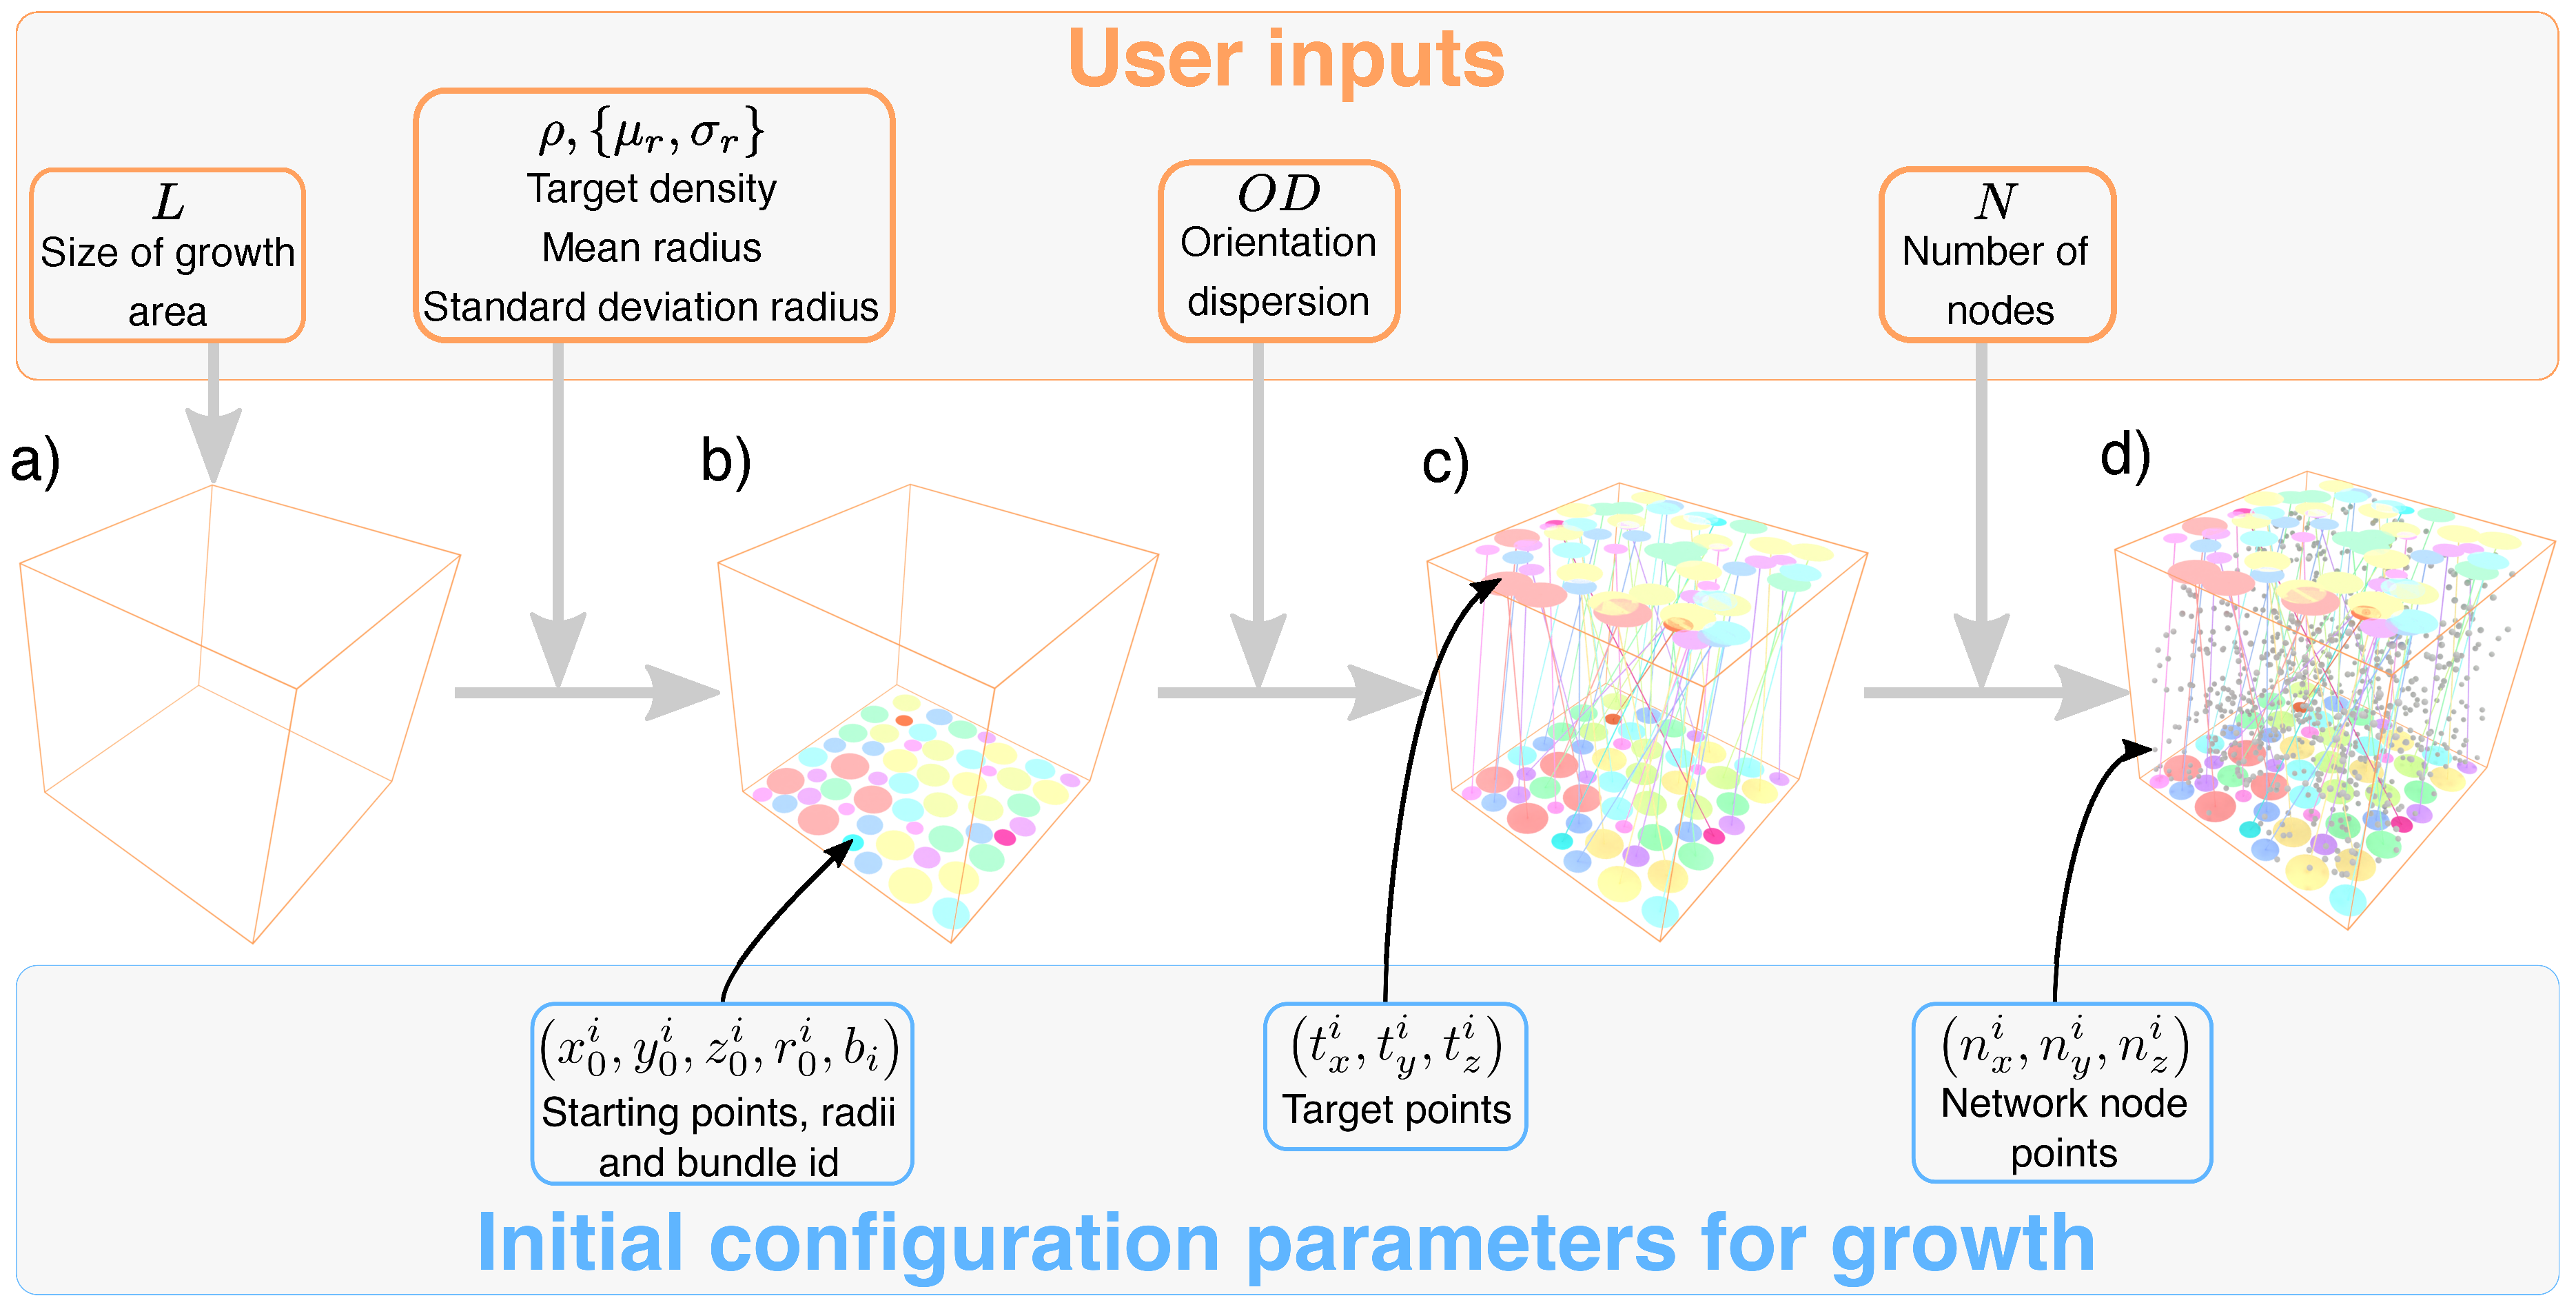
\includegraphics[width=\textwidth]{figures/config/method_inputs_only.eps}
  \caption[Inputs to the \ac{ConFiG} algorithm]{Inputs to the \ac{ConFiG} algorithm for the single bundle case. $L$ defines the size of the area of that the growth will take place in. The target density and fibre radius distribution govern the generation of starting points for each fibre by packing in 2D. Orientation dispersion parameters govern the generation of target points corresponding to each starting point. $N$ defines the number of nodes to use when generating the network. In the case of multiple bundles, starting and target points are generated for each bundle and then combined into the same space which is filled with nodes for the network. }
  \label{fig:config_inputs}
\end{figure}

First, Step 1 is broken down in to three substeps as outlined in \Cref{fig:config_inputs}:
\begin{description}
  \item [STEP 1.1] Generate fibre starting points (~\Cref{fig:config_inputs}a-b). To generate a starting point for each fibre to grow from, \ac{ConFiG} packs circles with the desired diameter distribution up to the target density (defined in terms of the desired fibre volume fraction) in 2D, following the approach taken in \cite{Hall2009}.

  \item [STEP 1.2] Generate fibre target points (~\Cref{fig:config_inputs}c). To encode the desired orientation distribution, each fibre has a direction drawn from the target distribution which gives a target point for the fibre to grow towards. As a demonstration of the flexibility of the framework, in this work we use the Watson distribution \cite{Mardia2008} for isotropic dispersion and the elliptically symmetric angular Gaussian distribution \cite{Paine2018} for anisotropic orientation dispersion, however other orientation distributions can be defined according to the user’s needs.

  \item [STEP 1.3] Generate growth nodes (~\Cref{fig:config_inputs}d). \ac{ConFiG} uses a set of pseudorandomly placed points (nodes) to sample the space and encode which regions are occupied by existing fibres. This simplifies collision checking making growth more efficient than a direct collision detection approach involving growing each fibre one small step at a time and checking collisions with existing fibres \cite{Callaghan2019}.
\end{description}

\begin{figure}[h!]
  \centering
  \includegraphics[width=\textwidth]{figures/config/method_without_inputs1.eps}
  \caption[Overview of the \ac{ConFiG} growth algorithm]{Overview of the basic growth algorithm in \ac{ConFiG}. In this example, three fibres are shown with a growth network that only contains relevant nodes for the sake of visualisation.  From the set of nodes, a network is constructed using the Delaunay triangulation. Each fibre then grows from node to node, along any edge connected to the current node. The node moved to will be the node with the lowest cost. Once a fibre segment has grown, the network nodes are updated to store information about which nodes are occupied or near to an existing fibres. This contributes to the cost function for any future fibres, penalising moving to nodes too close to existing fibres.  It is not possible to move to any node now inside a fibre as indicated by the removal of this edges from the network (pairs of blue arrows show where this is happening). The next fibres grow, now avoiding existing fibres until all fibres have finished.}
  \label{fig:config_algorithm}
\end{figure}

Second, Step 2, the main growth algorithm, is broken down into a series of substeps as outlined in \Cref{fig:config_algorithm}:
\begin{description}
  \item [STEP 2.1] Create growth network (~\Cref{fig:config_algorithm}a\&b). In order to encode which nodes a fibre can move to from any other node, the growth nodes are connected using the Delaunay triangulation.

  \item [STEP 2.2] Grow one fibre step (~\Cref{fig:config_algorithm}c-e). Fibres grow one-by-one in a random order along this network towards their target points while avoiding existing fibres. During growth, a fibre must choose in which direction it should grow. This direction is chosen in \ac{ConFiG} by following a cost function motivated by biological axonal guidance mechanisms (~\Cref{fig:config_algorithm}d), described in \Cref{sec:config_chemoattraction,sec:config_fasciculation}.

  \item [STEP 2.3] Update the network (~\Cref{fig:config_algorithm}f). The growth network is updated in order to store the information about the space this fibre is occupying so that future fibres can avoid it. The simplest way to do this is to store the minimum distance from each node in the network to any existing fibre as in \cite{Callaghan2019}. Additionally, another biologically motivated network updating strategy is described in \Cref{sec:config_dynam_growth}.

  \item [STEP 2.4] Repeat steps 2.2 and 2.3 until fibre reaches target (~\Cref{fig:config_algorithm}g). By default in \ac{ConFiG}, each fibre will grow completely before the next one starts, meaning that step 5 only needs to be performed once the fibre has finished growing. If fibres are allowed to grow concurrently, step 5 must be performed after each growth step.

  \item [STEP 2.5] Repeat steps 2.2-2.4 for remaining fibres (~\Cref{fig:config_algorithm}h-i). As noted in \Cref{fig:config_algorithm} (e-h), as the network is updated, more and more nodes become inaccessible making the network sparser. This means that some fibres may reach a point from which they cannot grow any further and will become stuck. Biologically inspired mechanisms designed to address this point are described in \Cref{sec:config_fibre_collapse,sec:config_dynam_growth}.
\end{description}

Finally, Step 3, the meshing procedure, is briefly described below and in further detail in \Cref{sec:ipmi_step3_meshing}:
\begin{description}
  \item [STEP 3] Generate 3D fibre meshes. After the growth process, each fibre will be represented by a series of connected 3D points and corresponding diameters at each point. In order to simulate diffusion \ac{MRI} signals, these fibre skeleta need to be turned into 3D meshes. \ac{ConFiG} uses a meshing procedure designed to eliminate overlap between fibres.
\end{description}

The remainder of this section outlines the biological process governing real axonal growth, and how these processes motivated the final implementation of the \ac{ConFiG} algorithm.
\end{comment}

\subsection{Biological motivation for \acs{ConFiG}}
\label{sec:config_biol_motiv}
In nature, axons grow following chemical cues in their environment through various mechanisms which either attract or repel fibres to guide their growth \cite{Dent2011,Lowery2009,Mortimer2008,Polleux2010,Price2017,Rauch2013,Sakisaka2005}. In an attempt to emulate real axonal growth, mechanisms motivated by the following guidance processes have been integrated into \ac{ConFiG}:
\begin{itemize}
  \item Chemoattraction – the process by which fibres are attracted to diffusible chemical cues in their environment \cite{Price2017,Mortimer2008}.
  \item Fibre collapse – a response to a chemorepulsive source whereby a fibre withdraws and regrows in a different direction \cite{Rauch2013}.
  \item Cell adhesion molecules – chemical signals on the surface of cells which guide axons that come into contact with them \cite{Sakisaka2005}.
  \item Fasciculation – the process by which multiple axons come together to form bundles \cite{Price2017,Smit2017}.
\end{itemize}
The following sections detail how mechanisms motivated by these biological processes are implemented in \ac{ConFiG} while \Cref{fig:config_chemoattraction,fig:config_dynam_growth,fig:config_fasciculation} illustrate these biological processes alongside their \ac{ConFiG} counterparts.

\subsubsection{Chemoattraction}
\label{sec:config_chemoattraction}
As a fibre grows it must choose in which direction it will move. One of the main processes governing the guidance of real axons is chemotropism; a process by which axons respond to diffusible chemical cues in their environment. One key chemotropic mechanism is chemoattraction, in which fibres are attracted along a chemical gradient towards a target region \cite{Price2017}.

\begin{figure}
  \centering
  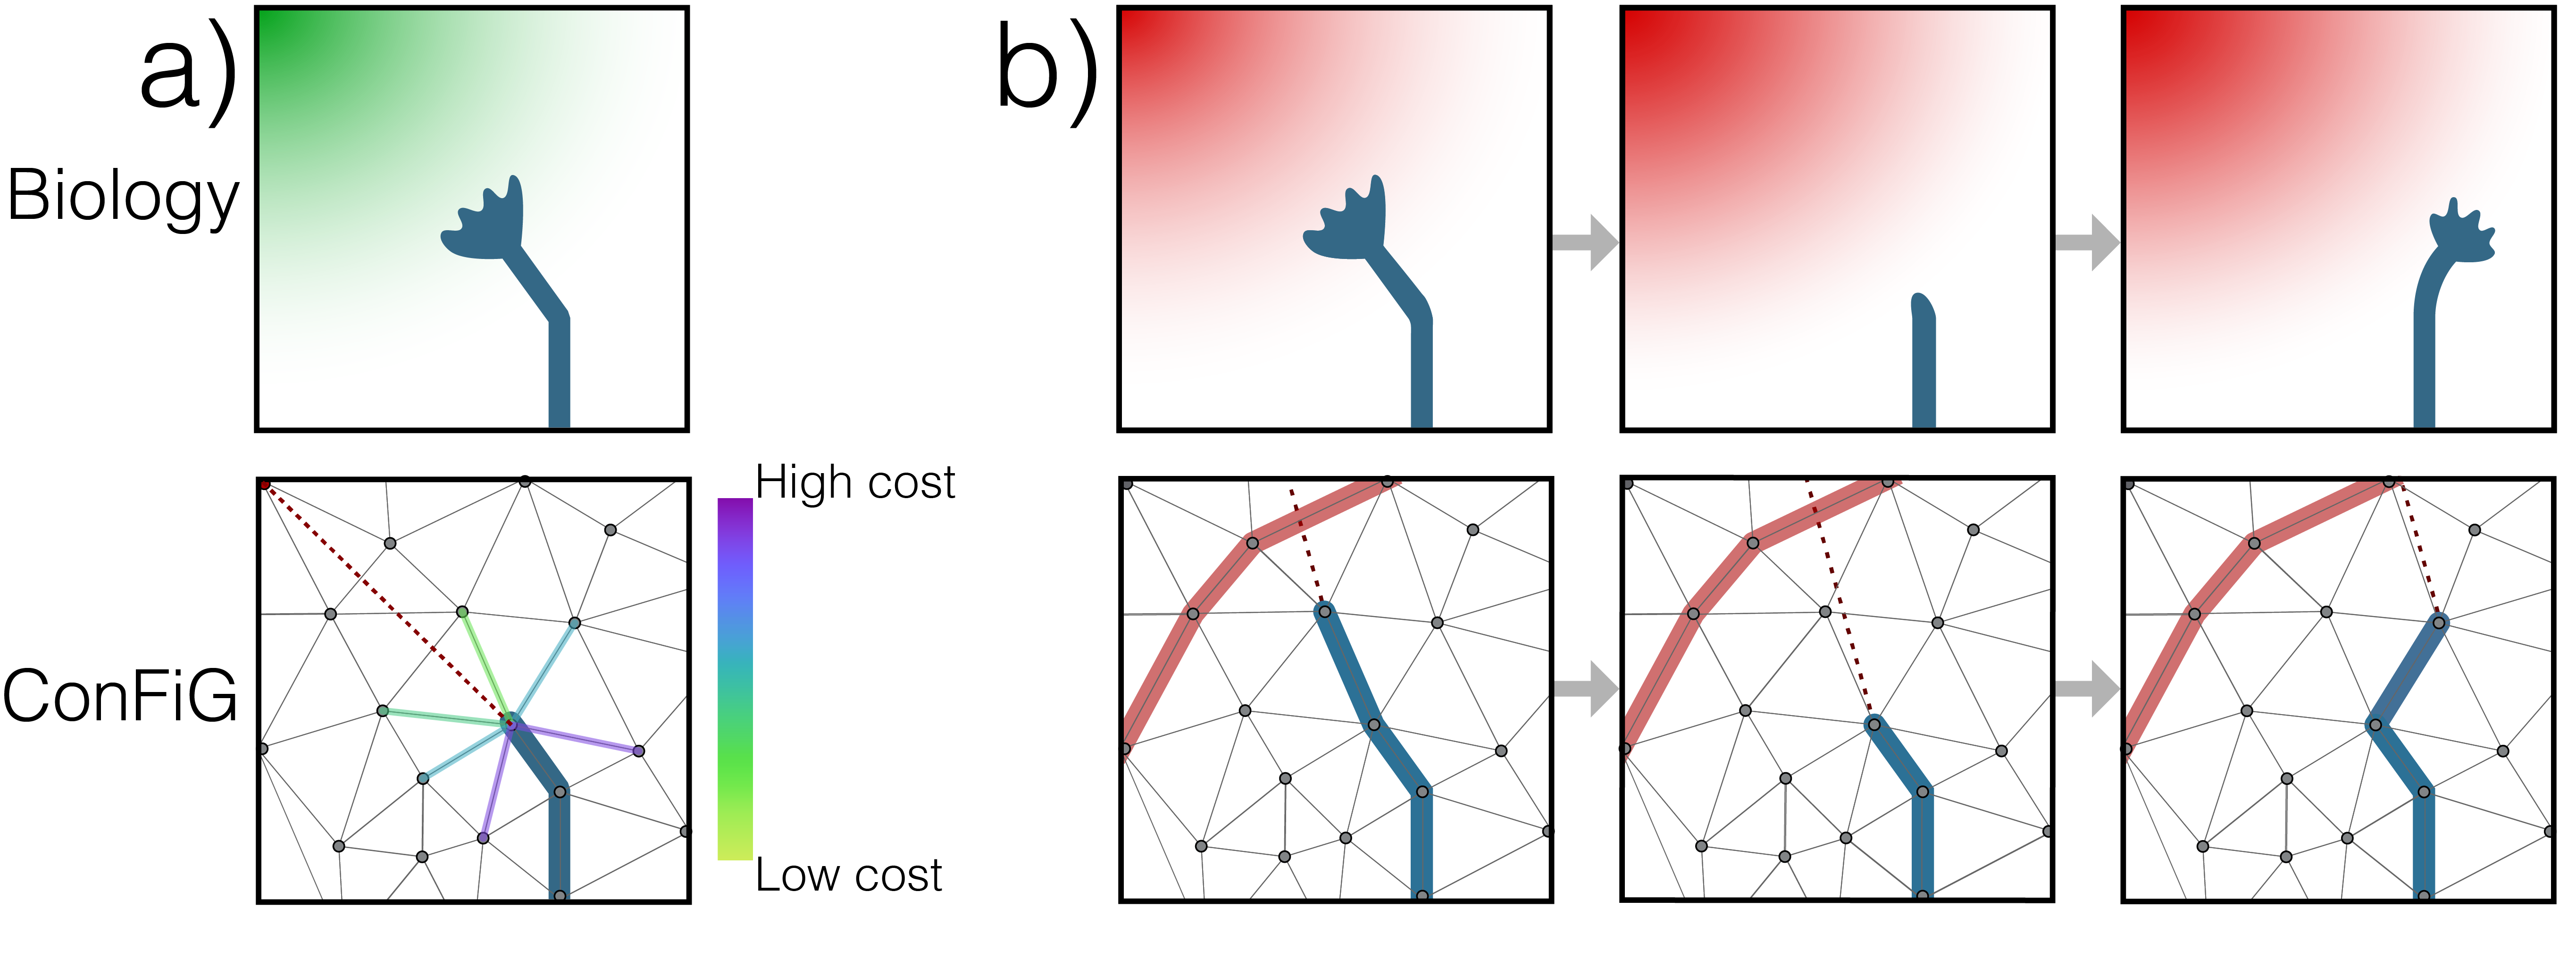
\includegraphics[width=\textwidth]{figures/config/biological_target+cam-01.png}
  \caption[Illustration of the chemoattraction process]{Illustration of two of the biological motivations and how they are implemented in \ac{ConFiG}. a) Growth towards the target is enforced by means of a cost function encouraging growth towards the target point. b) Fibre collapse is implemented by allowing the fibre to move backwards if it reaches a node from which there are no viable steps. The biological figures are adapted from \cite{Price2017}}
  \label{fig:config_chemoattraction}
\end{figure}

To approximate this chemoattractive mechanism, each fibre is encouraged to grow towards its target point (i.e. the target point acts like a chemoattractive source). This is the same guidance mechanism in the preliminary fibre growth algorithm presented in \Cref{sec:ipmi_step2_growth}.
The chemoattractive mechanism and its \ac{ConFiG} counterpart are illustrated in \Cref{fig:config_chemoattraction}a.

From any node in the growth network, the fibre will move along an edge that takes it towards its target while avoiding existing fibres according to a cost function \cite{Callaghan2019}.
From a starting node, $s$, the candidate nodes, $c$, that the fibre can move to are any nodes that share an edge with $s$. In addition to its position, each network node stores the maximum fibre diameter, $d_c$, that can be sustained at that node without intersecting another fibre. The fibre will move to a candidate node according to a cost function consisting of two terms; $l_t$, which penalises taking very large steps or moving away from the target point, $t$, and $l_d$, which penalises moving to a position where $d_c$ is low meaning that the fibre will have to shrink. The cost function for a fibre at a position, $s$, to move to a candidate node, $c$, given a target point, $t$, is
\begin{align}
  l &= l_t+fl_d  \,,\label{eq:original_cost}\\
      \mathrm{where}\nonumber\\
  l_t &=  \frac{1}{2} \cdot \frac{\|s-c\|}{1+ \|s-c\|} \cdot \left(1- \frac{\left(\left(c-s\right) \cdot \left(t-s\right)\right)}{\|c-s\|\|t-s\|}\right)\,, \label{eq:original_lt}\\
  l_d &=\mathrm{max}\left(0, \frac{1}{d_0} \left(d_0 - d_c \right)\right) \,. \label{eq:original_ld}
\end{align}
Here, $d_0$ is the target diameter of the fibre and $f$ is a weighting factor between the two terms. In this work, $f$ is fixed to 0.2 to more strongly weight growth towards the target.

The next node for a fibre will be the candidate node which has the lowest cost according to \Cref{eq:original_cost}. This method of finding a path through the triangulation by choosing the lowest cost node at each position amounts to a greedy best-first pathfinding approach with a heuristic given by \Cref{eq:original_cost}.

Growing fibres along the network using just this chemoattractive mechanism is the minimal implementation of \ac{ConFiG} that will generate substrates to try and meet the morphological inputs. There are some limitations to this minimal approach however; the greedy growth and the sparse sampling of the space means that fibres can grow into regions from which they cannot grow further and become stuck. Additionally, in this approach, fibres grow independently of one another, whereas real fibres grow forming bundles in the process known as fasciculation.

\Cref{sec:config_fibre_collapse,sec:config_dynam_growth,sec:config_fasciculation} describe further mechanisms which were added to enable \ac{ConFiG} to address these limitations in order to meet more complex morphological priors (e.g. high density and orientation dispersion together).

\subsubsection{Fibre collapse}
\label{sec:config_fibre_collapse}
As mentioned in \Cref{sec:config_biol_motiv}, in \ac{ConFiG} a fibre can become stuck when there are no possible next steps because all neighbouring nodes are inaccessible. In an attempt to ameliorate this a process mimicking fibre collapse was implemented, illustrated in \Cref{fig:config_chemoattraction}b.

In \ac{ConFiG} fibre collapse, the fibre will move back by an initial distance, $g_0$, and regrow from there avoiding any nodes in the route it took previously. If the fibre becomes stuck again, it will move back by a further distance, $g_0+ \delta$, where $\delta$ is the additional distance to step back. This process is repeated until the fibre reaches the target or gets stuck a user-defined maximum number of times. In this work, $g_0=\SI{2}{\micro\metre}$  and $\delta=\SI{5}{\micro\metre}$ in an approximation of the biological fibre collapse process investigated by Rauch et al. \cite{Rauch2013} who show fibres collapsing up to \SI{25}{\micro\metre} back towards the soma. The maximum number of steps back is set to 5, meaning that the maximum step back is \SI{27}{\micro\metre}, in line with real fibres. If there is no possible route after 5 attempts then the fibre will stop growing and will be removed from the phantom. This process of removing stuck fibres means that the resulting substrate may not always have the same density as the input desired fibre density.

\subsubsection{Dynamic growth network}
\label{sec:config_dynam_growth}

\begin{figure}
  \centering
  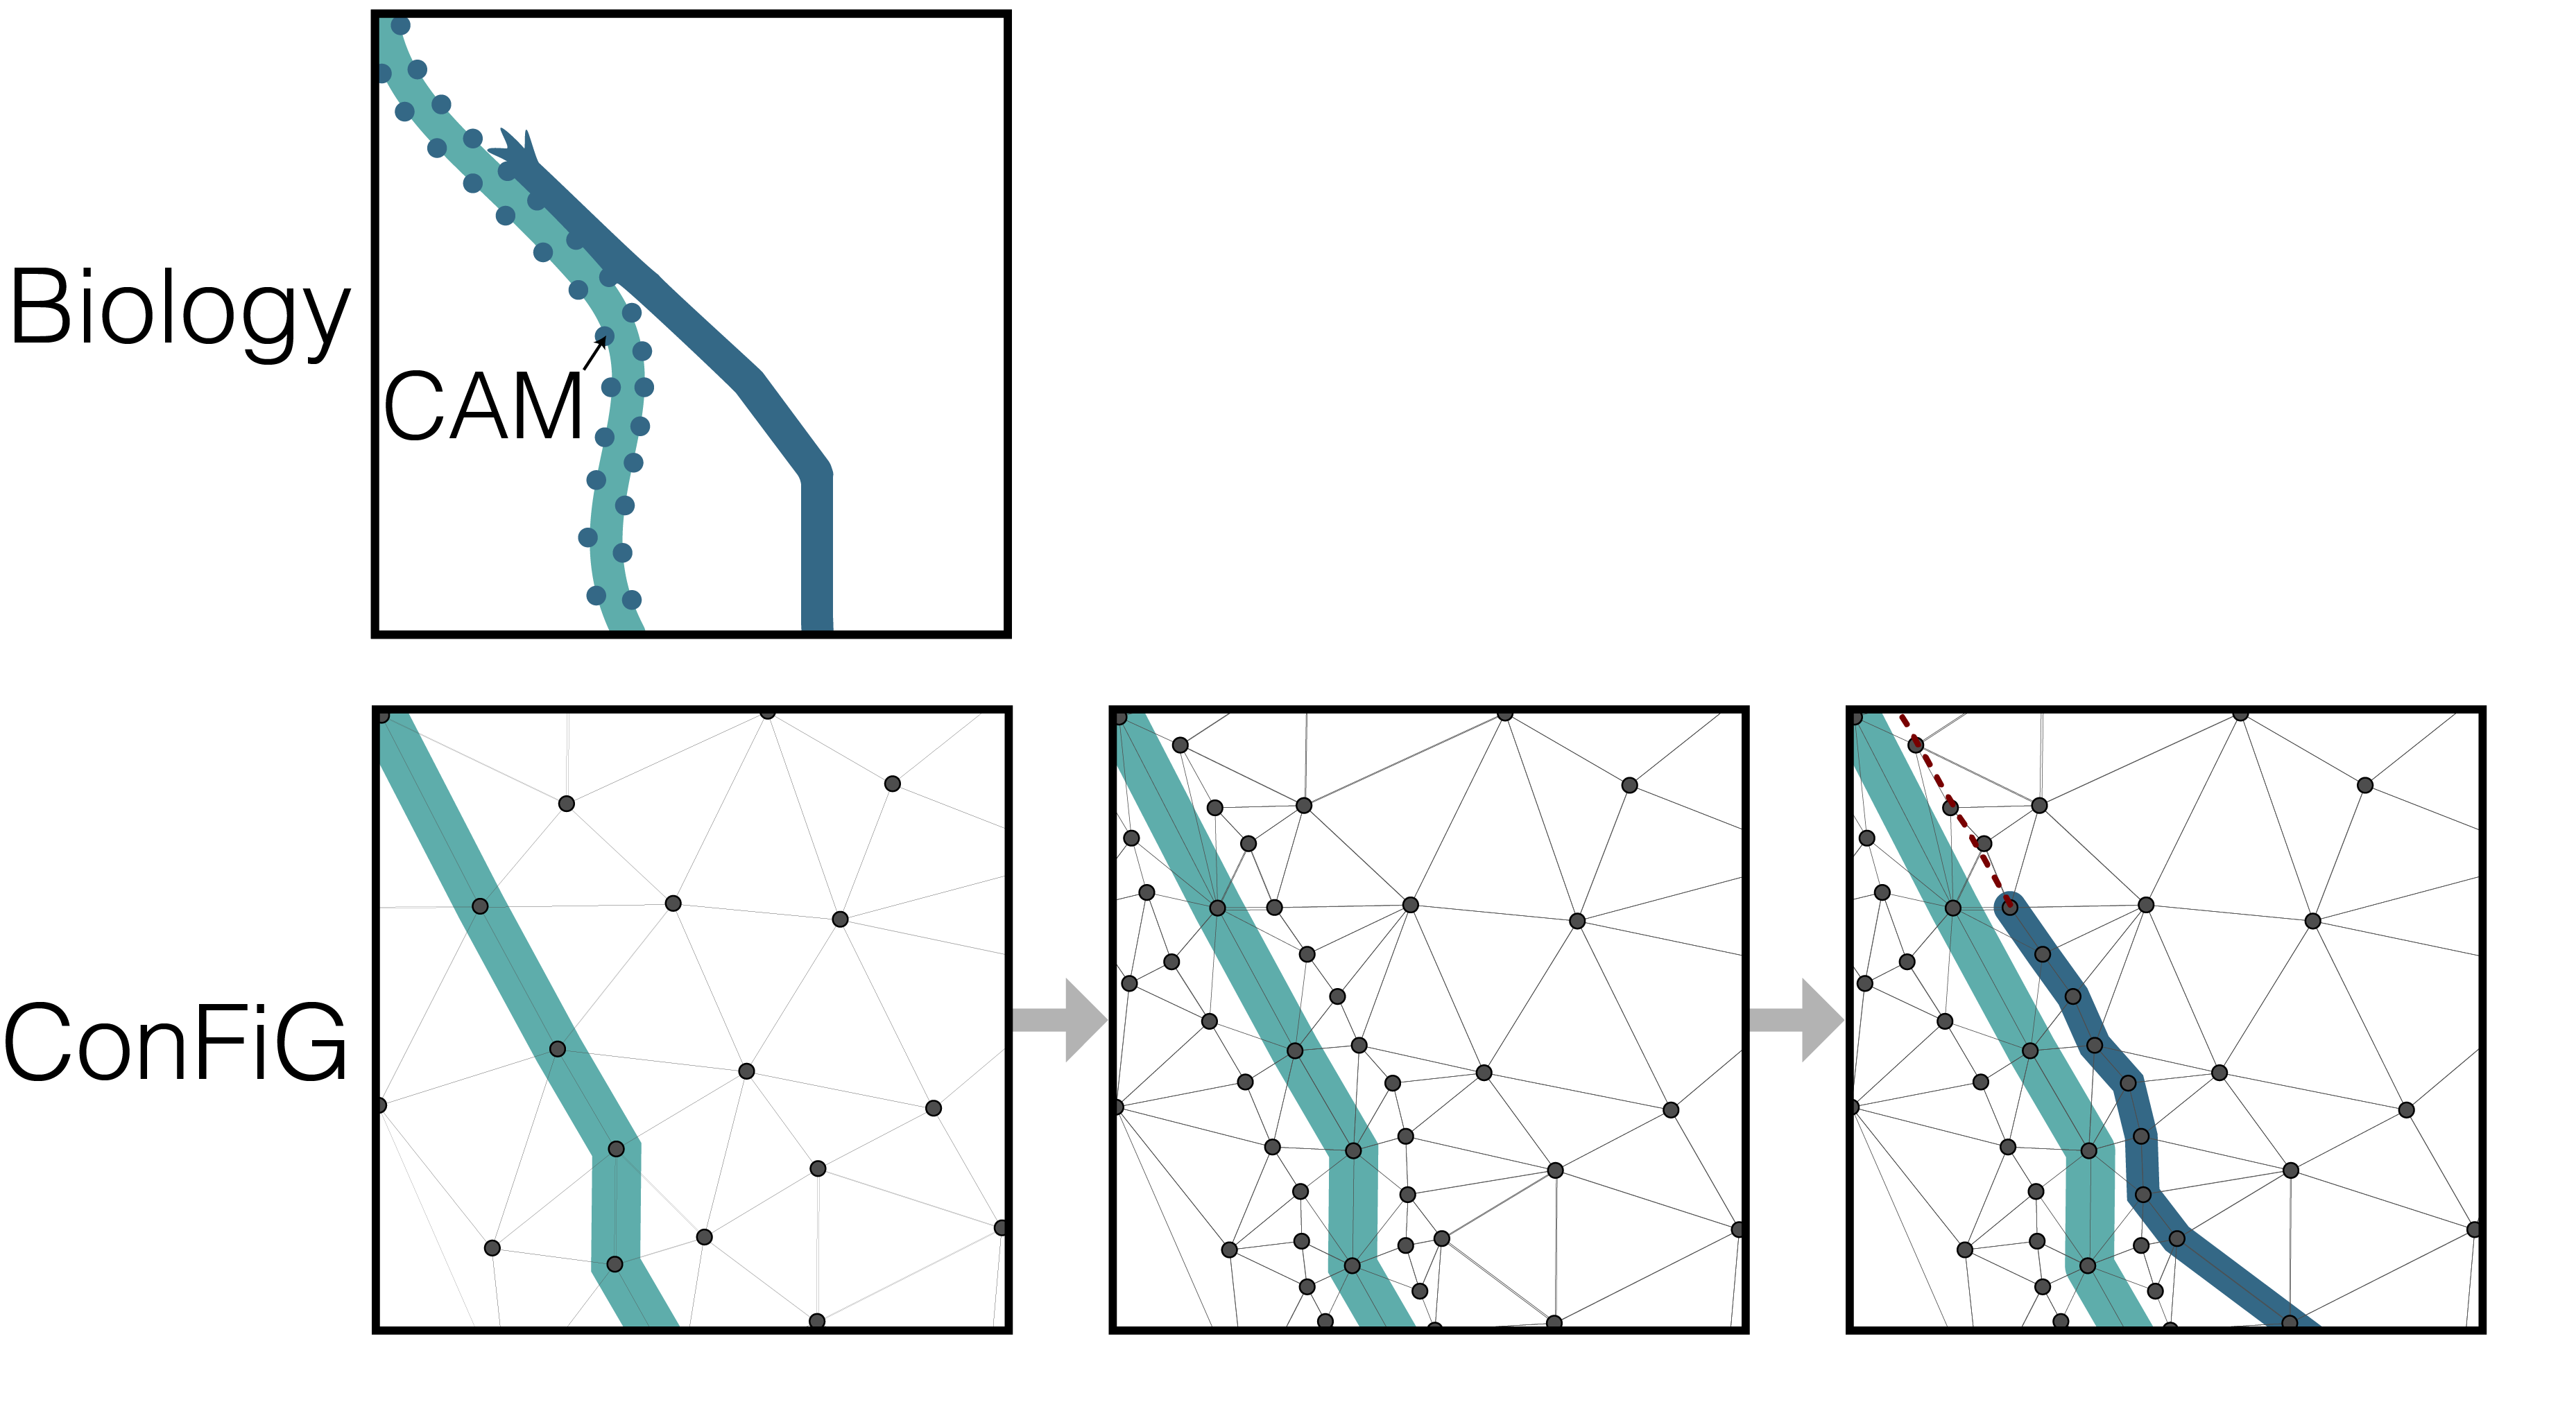
\includegraphics[width=0.8\textwidth]{figures/config/biological_cam.png}
  \caption[Illustration of the contact guidance mechanism]{Illustration of the contact guidance axonal growth mechanism and the dynamic growth network implemented in \ac{ConFiG}. The dynamic growth network is implemented as a set of points added around each fibre after growth, enable future fibres to more easily grow along/around existing fibres.}
  \label{fig:config_dynam_growth}
\end{figure}

In the preliminary implementation of \ac{ConFiG} \cite{Callaghan2019}, the network nodes were initialised pseudorandomly within the growth region and once initialised, the growth network was static, meaning that the nodes and edges of the network were fixed. This limited the growth to the specific instantiation of the network and it could not adapt to where fibres were once they had grown. Furthermore, as illustrated in \Cref{fig:ipmi_config_algorithm}, as fibres grow, many nodes become inaccessible due to being within fibres meaning that the network becomes gradually sparser.

A dynamic growth network was implemented to ameliorate these effects. Now, once a fibre has reached the target, a number of nodes, $N_{added}$, are generated around the path of the fibre. This gives a denser sampling of the space in regions in which fibres exist and serves to give subsequent fibres more nodes to use to grow along or around that fibre, helping to increase the achievable density by limiting the number of fibres which get stuck. In this work, where the dynamic network is used, $N_{added}=2500$.

This is also loosely motivated by the contact guidance mechanism in which axons are attracted to or repelled by chemical cues on the surface of other cells, known as \acp{CAM}. Here, the added points act like \acp{CAM} meaning that a future fibre which grows can use these points near to the fibre to grow around or along it as if it were following contact guidance cues. \Cref{fig:config_dynam_growth} shows how \acp{CAM} work in biological axonal growth alongside the \ac{ConFiG} dynamic network, illustrating the parallels between the two.

\subsubsection{Axon fasciculation}
\label{sec:config_fasciculation}

\begin{figure}
  \centering
  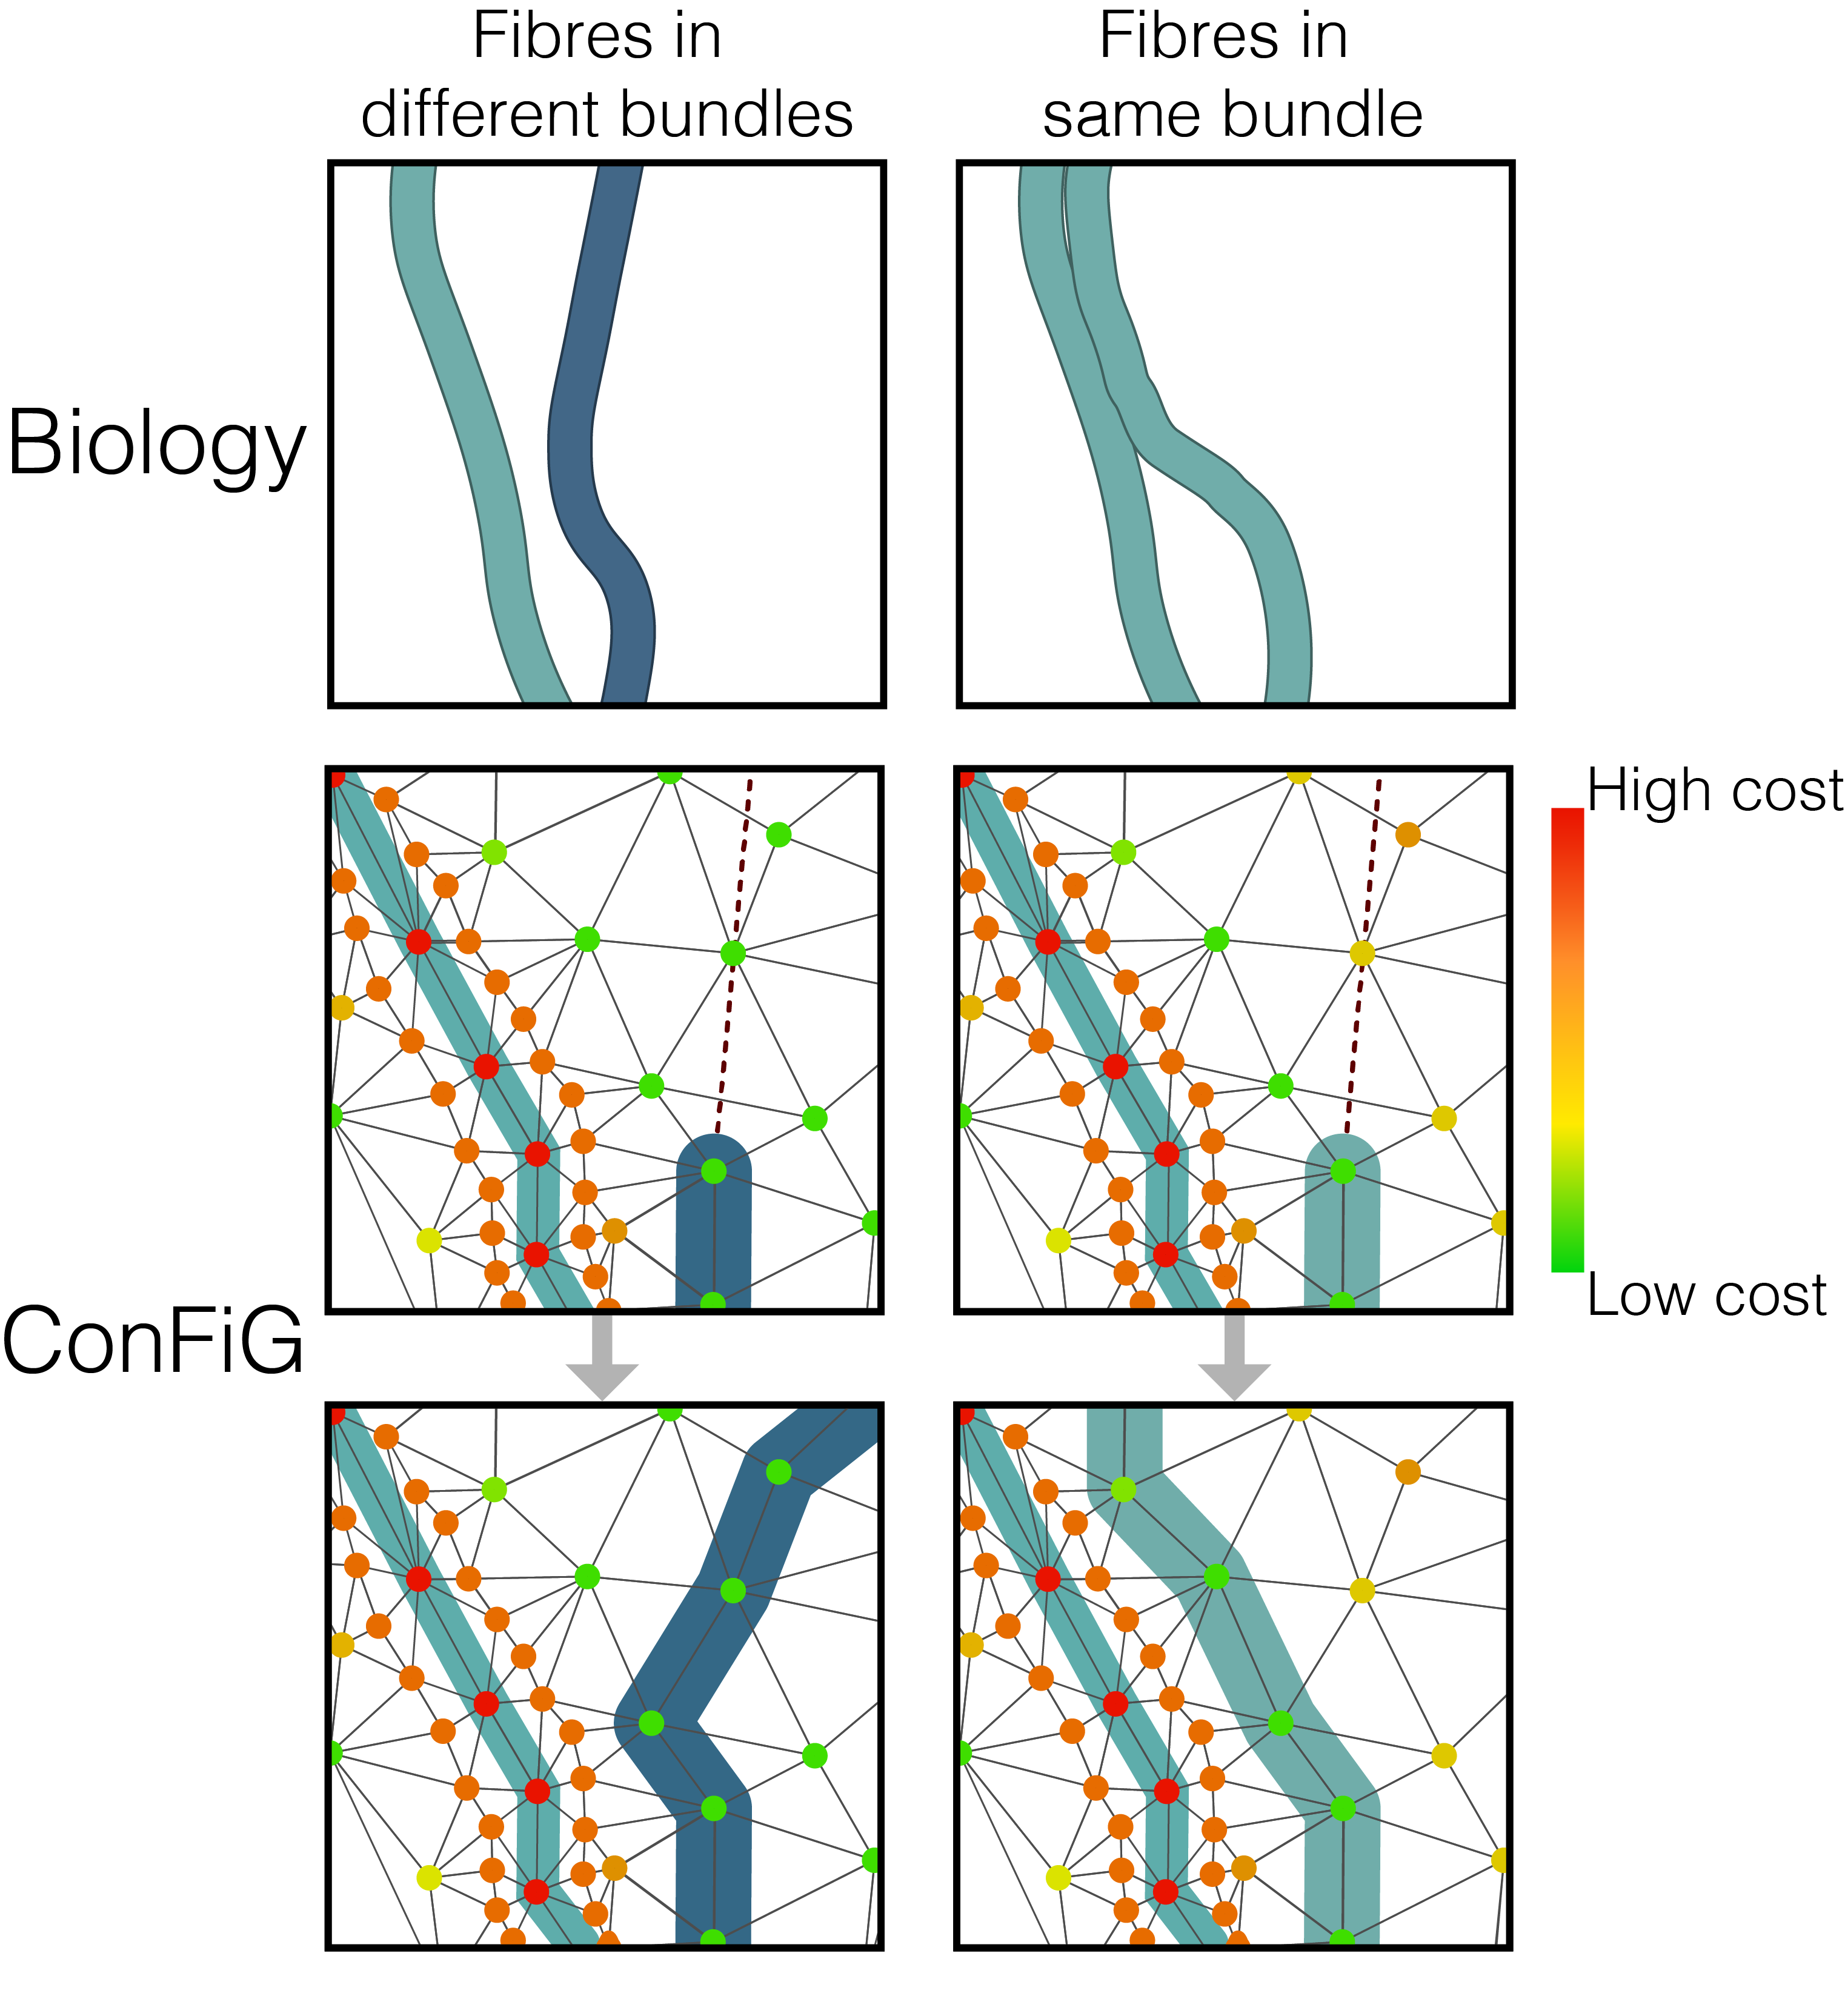
\includegraphics[width=0.5\textwidth]{figures/config/biological_fasciculate.png}
  \caption[Illustraction of the fasciculation process]{Illustration of how the labelled pathway hypothesis is expected to work in biology and its \ac{ConFiG} counterpart. Fasciculation is implemented using the cost function term in Eq. 1 which means that fibres in the same bundle are encouraged to stay close to one another.}
  \label{fig:config_fasciculation}
\end{figure}

One particular role \acp{CAM} play is in axon fasciculation, the process in which axons follow a so-called pioneer axon closely, forming a bundle \cite{Price2017,Sakisaka2005}. To mimic the process of axon fasciculation, the term in the cost function penalising moving into regions in which the fibre had to shrink, $l_d$ \Cref{eq:original_ld}, was altered to be conditional on which fibre bundle is closest.

A fibre, $f$, with a target diameter, $d_0$, moving to a candidate node, $c$, which has a maximum sustainable diameter $d_c$ will now have $l_d$ given by:
\begin{equation}
  \label{eq:updated_ld}
  l_d = \begin{cases}
    \max\left(0, \frac{1}{d_0} \left(d_0 - d_c\right)\right) & \text{if } b_c \neq b_f \\
    \mathrm{abs}\left(\frac{1}{d_0} \left(d_0 - d_c\right)\right) & \text{if } b_c = b_f
    \end{cases}
\end{equation}

Where $b_f$ is an index identifying the bundle that fibre $f$ belongs to and $b_c$ is the index of the bundle that is closest to $c$ (i.e. the index of the bundle of the fibre that set $d_c$). This means that when $c$ is closest to the same bundle as $f$, the cost function penalises moving away from that bundle as well as shrinkage, whereas when the bundles differ, it only penalises shrinkage.

This new form of the cost function encourages fibres of the same bundle to stick together while still avoiding fibres of different bundles, inspired by the labelled pathway hypothesis, which states that axons join different fascicles based on different \acp{CAM} expressed on the fibres \cite{Price2017}. In this case, bundle indices $b_c$ and $b_f$ act like different identifying \acp{CAM}. \Cref{fig:config_fasciculation} shows how this fasciculation process is expected to happen in biology alongside how the improved cost function encourages a similar process in \ac{ConFiG}.

\subsubsection{Global optimisation}
\label{sec:config_global_optimisation}
Since the growth of fibres in \ac{ConFiG} takes place on a discrete network of points, the final positions of fibre nodes may be suboptimal for achieving the maximum density. In other words, certain fibres’ nodes may be closer to other fibres than they would ideally be in order to reach their target diameter (i.e. the fibre has had to shrink its diameter at that node).

To mitigate against this, a global optimisation step was added at the end of the growth in a procedure similar to MEDUSA \cite{Ginsburger2019}. For each point, $i$, that is part of a fibre, its nearest $n$ neighbours $(j \in NN(i))$ from other fibres are found; in this work $n=10$. The distance to all of the neighbours is found and the point’s position is updated from these distances according to the update vector, $\vec{u}_i$
\begin{equation}
  \label{eq:global_opt_update_vec}
\vec{u}_i= \sum_{j \in NN(i)} D(i,j) \cdot \left(\vec{p}_i - \vec{p}_j\right) \,,
\end{equation}
where $\vec{p}_i$ and $\vec{p}_j$ are the locations of point $i$ and $j$. $D(i,j)$ is the function determining whether the interaction is repulsive or attractive:
\begin{equation}
  \label{eq:global_opt_Dij}
  D(i, j) = \mathrm{sgn}\left(r_i + r_j - \|\vec{p}_i - \vec{p}_j\|\right) \,.
\end{equation}

Here, $\mathrm{sgn}$ is the signum function and $r_i$ and $r_j$ are the target radii of point $i$ and $j$. The sum of these radii is the desired distance between the points since that means the fibres are just touching. $D(i,j)$ imposes that the force is repulsive if the points are closer together than the desired radius and attractive if they are further apart. The update vector is scaled such that if $\|\vec{u}_i\| > 0.2r_i$, the update vector is rescaled so that $\|\vec{u}_i\|=0.2r_i$. This acts to prevent the update vector from becoming very large.

There is some biological evidence that this kind of interaction between fibres is important in the fasciculation process. The fasciculation process described in \Cref{sec:config_fasciculation} relies on \acp{CAM} detected at the tip of a growing axon, however some studies provide evidence for fasciculation through interactions along axon shafts, known as zippering \cite{Barry2010,Smit2017,Voyiadjis2011}. In zippering, nearby axon shafts attract one another to form more closely packed fascicles, which is a similar process to the global optimisation process in \ac{ConFiG}.

\subsection{Summary of \acs{ConFiG} input parameters}
\label{sec:config_summary_of_input}
\Cref{tab:config_parameters} summarises the key parameters that govern the generation of \ac{ConFiG} phantoms. Parameters are split into those which define the target microstructural morphology and those which define the instantiation of the growth algorithm. For each parameter, the theoretical range is reported alongside the practical range that has been tested so far. This is due to stochastic nature of the algorithm and the interdependence of the parameters. For instance a very large substrate is possible if very large fibres are chosen, but likely impossible with very small fibres since this will require a very large number of fibres and run into memory limitations.

\begin{table}[!h]
  \footnotesize
  \centering
  \caption{Summary of \ac{ConFiG} parameters split into parameters which define the target microstructural morphology and parameters which define the instantiation of the growth algorithm. For each parameter the theoretical range is reported as well as the practical range that has been tested so far.}
  \label{tab:config_parameters}
  \begin{tabular}{cccr@{}lb{2cm}c}
    \toprule
     \multicolumn{2}{c}{\textbf{Parameter}} & \multicolumn{3}{c}{\textbf{Meaning}} & \centering \textbf{Theoretical Range} & \textbf{Practical Limits Tested} \\ \midrule
     \multirow{7}{*}{\rotatebox[origin=c]{90}{\parbox[c]{3.5cm}{\centering \textbf{Target microstructure parameters}}}}
     & $L$ & \multicolumn{3}{c}{Size of growth region} & \centering $\mathbb{R}_+^3$ & $[0,0,0] \rightarrow [50,50,50]$ \si{\micro\metre} \\
     &$\rho$& \multicolumn{3}{c}{Fibre volume fraction}& \centering$[0,1]$ & $[0,0.8]$ \\
     & $\mu_r$& \multicolumn{3}{c}{Mean radius}& \centering $\mathbb{R}_+$&  $[0.5,2]$ \si{\micro\metre}\\
     & $\sigma_r$& \multicolumn{3}{c}{Standard deviation radius}& \centering$\mathbb{R}_+$& $[0.1,0.5]$ \si{\micro\metre}\\
     & \multirow{3}{*}{$GAD$} & \multirow{3}{2cm}{\centering Global angular dispersion} & Watson & $: \kappa$ & \centering$\mathbb{R}_+$& $[4,100]$ \\
     & & & \multirow{2}{*}{ESAG $\Big\{\!$}& $\ \mu$ & \centering$\mathbb{R}_+$ & $[2,10]$ \\
     & & & & $\ \gamma$ & \centering$\mathbb{R}_+^2$ & $[2,2] \rightarrow [10,10]$\\ \midrule
    \multirow{4}{*}{\rotatebox[origin=c]{90}{\parbox[c]{3cm}{\centering \textbf{Growth algorithm parameters}}}} & $N$ & \multicolumn{3}{c}{Number of growth nodes} & \centering$\mathbb{N}$ & $[0,10^7]$ \\
    & $f$ & \multicolumn{3}{c}{Cost function weighting term} & \centering$[0,1]$ & $[0,0.5]$  \\
    & \multirow{2}{*}{$g_0, \delta$} & \multicolumn{3}{c}{\multirow{2}{4cm}{\centering Fibre collapse initial and subsequent step length}} & \centering\multirow{2}{*}{$\mathbb{R}_+$} & \multirow{2}{*}{$[1,5],[1,5]$ \si{\micro\metre}} \\
    & & & & & \\
    & \multirow{2}{*}{$N_{\text{added}}$} & \multicolumn{3}{c}{\multirow{2}{4cm}{\centering Dynamic network no. nodes added}} & \centering\multirow{2}{*}{$\mathbb{N}$} & \multirow{2}{*}{$[0,5000]$}\\
    & & & & & \\ \bottomrule
  \end{tabular}
\end{table}

\section{Experiments}
\label{sec:config_experiments}
In order to assess the performance of \ac{ConFiG}, a range of experiments were performed. The first set of experiments were performed in order to explore the impact of each of the biologically inspired growth mechanisms. Another set of experiments aimed to show that \ac{ConFiG} is able to generate substrates with realistic microstructure by comparing generated substrates with real tissue. Additionally, the relationship between the user-specified target morphology and the final output morphology was investigated by comparing resulting phantoms to their inputs (target density and orientation distribution). Finally, a simulation experiment was performed to assess how well \ac{ConFiG} phantoms can be used to generate realistic diffusion \ac{MRI} data. The rest of this section outlines these experiments.

\subsection{Testing the performance of \acs{ConFiG}}
\label{sec:config_test_perf}
In order to test how each of the biological mechanisms proposed in \Cref{sec:config_methods} impacted on the resulting phantoms, an experiment was devised to measure how phantoms changed when each mechanism was introduced. Four scenarios of interest were generated using several variants of the \ac{ConFiG} algorithm that included these mechanisms either one at a time or all at once, attempting to grow phantoms as densely as possible:
\begin{itemize}
  \item one bundle of parallel fibres, target density 75\%
  \item one bundle with Watson distributed fibres $(\kappa=8)$, target density 75\%
  \item two perpendicular crossing bundles, intra-bundle target density 40\%
  \item three mutually perpendicular crossing bundles, intra-bundle target density 30\%
\end{itemize}
These target densities were chosen to ensure that the centre of the phantom (i.e. the crossing region for crossed bundles) had a high target density whilst ensuring that each bundle had a reasonable number of fibres to begin with (>50).

The \ac{ConFiG} variants were tested by generating phantoms for each of the scenarios starting with the same initial conditions. Each phantom was generated 5 times with a different random seed and results averaged across the seeds.

To investigate the impact of the biological mechanisms on \ac{dMRI} simulation, a comparison was made between real \ac{dMRI} signals and simulations from \ac{ConFiG} phantoms. The \acs{NODDI} model \cite{Zhang2012} was fitted to a \ac{WM} ROI in the corpus callosum of a \ac{HCP} \cite{VanEssen2012} subject to provide sensible input parameters (target fibre density and orientation dispersion) for \ac{ConFiG} to generate phantoms. We generated phantoms using the two extreme cases: the minimal growth case only using chemoattraction, and the complete \ac{ConFiG} algorithm using all mechanisms. Whilst the random nature of \ac{ConFiG} means that the resulting phantom will not have morphology exactly matching the input parameters, this approach ensured that the phantoms were reasonable for this proof of concept experiment.

The \ac{dMRI} signal was simulated in the phantoms using Camino \cite{Cook2006,Hall2009} with identical simulation conditions in both cases and the measurement scheme corresponding to the \ac{HCP} \ac{dMRI} sequence \cite{Sotiropoulos2013a}. An important consideration when performing \ac{dMRI} simulations is the size of the substrate relative to the diffusion length. The phantom should be large enough that it is bigger than the diffusion length, but not so large as to require excessive computational resources. Owing to the relatively long diffusion time (\SI{43}{\milli\second}) in the \ac{HCP} sequence, phantoms were extended with reflected copies \cite{Lee2019a,Fieremans2018} to increase their effective size relative to the diffusion length scale.

All \ac{dMRI} simulations in this work used a bulk diffusivity $D=\SI{2.0}{\micro\metre\squared\per\milli\second}$ in agreement with values used in similar Monte Carlo simulations \cite{Hall2009,Nilsson2009,Rensonnet2017} with $10^5$ spins and $2000$ timesteps. Standard Camino periodic boundaries were used \cite{Hall2009}, with \ac{dMRI} signal was generated from a central region 75\% the size of the total phantom to avoid boundary effects \cite{Panagiotaki2010}.


\subsection{Diffusion \acs{MRI} simulation}
\label{sec:config_diffusion_sim}
To qualitatively verify that the simulated diffusion \ac{MRI} signals from \ac{ConFiG} phantoms are realistic, simulated signals from \ac{ConFiG} phantoms were compared to real \ac{HCP} data \cite{Sotiropoulos2013a,VanEssen2012}.

In the real data, the \ac{FOD} was fit in each voxel using \ac{CSD} in MRTrix \cite{Tournier2019,Tournier2007}. Voxels were selected in regions of interest in the midbody of the \ac{CC} and the \ac{IC}, regions in which a single bundle of fibres is found from the FOD. A third voxel was selected in which three crossing fibre populations were found from visual inspection of the FOD.


In each voxel, the diffusion tensor was fit to the signal and the principal eigenvector used to define a major direction of diffusion in the voxel, $n$. From this, the normalised diffusion weighted signal was plotted against $|n\cdot G|$, where $G$ is the gradient direction. Additionally, the direction averaged signal was calculated for each b-shell.

To attempt to generate representative microstructure for each voxel using \ac{ConFiG}, the \ac{NODDI} model \cite{Zhang2012} was fitted to the average signal to give some initial parameters for \ac{ConFiG}. Most importantly, the value of $\kappa$ for the Watson distribution \cite{Mardia2008} estimated using \ac{NODDI} was used to initialise the orientation dispersion in the \ac{ConFiG} phantoms used to represent \ac{CC} ($\kappa=6.2$) and \ac{IC} $(\kappa=5.5)$ regions. To represent the \ac{TC} voxel, a phantom generated using three mutually perpendicular crossing bundles was used.

ConFiG phantoms were grown using these initial conditions and the diffusion \ac{MRI} signal simulated using the Camino Monte Carlo diffusion \ac{MRI} simulator \cite{Hall2009}. For each phantom, the same processing as with the real data was performed, finding the direction dependent and direction averaged signal per b-shell.

\subsection{3D signal visualisation}
\label{sec:config_3d_signal_vis}
In order to better understand how close the simulated signal is to the real signal, a new method for 3D visualisation of the signal was developed.
A 6th order \ac{SH} representation of the simulated signal was calculated for a given $b$-value and the surface plotted in 3D. On top of this, the real data for that $b$-value were plotted as points with a line projected along the gradient direction to the surface to show the distance between the real and simulated signals in that direction.
Each point is coloured red or blue depending on whether the measured signal is above or below the simulated signal respectively.

Since there is no guarantee that the microstructure is aligned similarly relative to the gradients in the \ac{ConFiG} phantom and real data (indeed, it is highly unlikely that they are), the Bingham-NODDI model \cite{Tariq2016} is fit to the both the real and simulated data to give a basis for each, defined by three orthogonal vectors: the principal diffusion direction $\mu_1$, the principal fanning direction $\mu_2$ and a vector mutually orthogonal to both of these, $\mu_3$, defined as $\mu_1 \times \mu_2$.

A rotation matrix is use to bring these two bases into alignment, defined as follows\footnote{This solution is based on \url{https://math.stackexchange.com/questions/1125203/finding-rotation-axis-and-angle-to-align-two-3d-vector-bases}}: The rotation matrix $R$ that brings a basis of unit vectors$(\vec{a}, \vec{b}, \vec{c})$ onto another basis $(\vec{d}, \vec{e}, \vec{f})$ must fulfil
\begin{align}
R\vec{\vphantom{t}a} &= \vec{d} & R\vec{b} &= \vec{\vphantom{t}e} & R\vec{\vphantom{t}c} &= \vec{f}\,.
\end{align}

This matrix can constructed through the addition of three dyads
\begin{equation}
  R = \vec{d}\,\vec{\vphantom{f}a} + \vec{\vphantom{f}e}\,\vec{b} + \vec{f}\,\vec{\vphantom{f}c} \,,
\end{equation}
which can be seen to work if we multiply through by one of the first basis vectors $R\vec{a} = \vec{d}\,\vec{\vphantom{f}a}\cdot\vec{\vphantom{f}a} = \vec{d}$, since $\vec{a}$ multiplied with itself gives unity and is orthogonal to $\vec{b}$ and $\vec{c}$.
Each of these dyads can be written as a 3x3 matrix using the vector direct product, giving the rotation matrix
\begin{equation}
R = \vec{d} \otimes \vec{\vphantom{f}a}^{\,T} + \vec{\vphantom{f}e} \otimes \vec{\vphantom{f}b}^{\,T} + \vec{f} \otimes \vec{\vphantom{f}c}^{\,T}\,,
\end{equation}
where $\otimes$ denotes the Kronecker product. This rotation matrix, $R$ is used to bring the simulated and real data into the same space for visualisation.


This approach to signal visualisation enables us to get a better feel for how close the signals are and whether there is any pattern to the discrepancy (for instance, is the measured signal high along one axis and low along another).
Besides its application here to see how close our simulated and real signals are, this could be a useful tool to see how fitting models are behaving. For instance plotting the data against a surface from a \ac{NODDI} fit may enable easy identification of cases where the isotropic orientation dispersion assumed in Watson-NODDI is a poor fit to the data and where Bingham-NODDI \cite{Tariq2016} may be better.
In this case of plotting data against a fit, the alignment approach described above does not need to be followed since the fitting parameters will already be in the same space as the real data.


\section{Results}
\label{sec:config_results}

\subsection{Impact of biological mechanisms}
\label{sec:config_result_impact_of_mechanisms}

\begin{figure}
  \centering
  \includegraphics[width=\textwidth]{figures/config/improvements_wfascicle_tight.eps}
  \caption[Impact of biological mechanisms in \ac{ConFiG}]{Demonstration of the impact of each biological growth mechanism on the density achievable with \ac{ConFiG}. Each bar shows the mean density for each proposed mechanism, error bars show $\pm$ standard error on the mean. MEDUSA values are estimated from Fig. 14 in Ginsberger et al. (Ginsburger et al., 2019).}
  \label{fig:config_res_improvements}
\end{figure}

Each of the proposed biological mechanisms enabled \ac{ConFiG} to generate phantoms with increased density over the minimal case of chemoattraction only, as is shown in \Cref{fig:config_res_improvements}. Global optimisation resulted in the largest improvement, 17-24\%, consistently giving a large improvement. Other improvements performed better for specific phantom configurations. For instance, fasciculation and the dynamic network produced only modest improvements in crossing fibre configurations (4-6\%), but performed well in the single bundle cases (11-14\%). Fibre collapse was particularly effective in the three perpendicular case, offering 10\% improvement.

\begin{figure}
  \centering
  \includegraphics[width=\textwidth]{figures/config/improvements_virthist.png}
  \caption[Impact of biological mechanisms on virtual histology]{Virtual histology demonstrating the impact of biologically inspired mechanism on the final phantom created for one of the parallel phantoms tested. This visually demonstrates the improvement in density. Leftmost image shows the phantom generated with all mechanisms in 3D and the cutting plane used to produce the virtual histology.  }
  \label{fig:config_res_improvements_virthist}
\end{figure}

\begin{figure}
  \centering
  \includegraphics[width=\textwidth]{figures/config/improvement_3drender.png}
  \caption[Impact of biological mechanisms on 3D phantoms]{Demonstration of the improvement in density achieved when using all mechanisms in \ac{ConFiG} compared to the minimal implementation using only chemoattraction. Colours chosen to match \Cref{fig:config_res_improvements}. }
  \label{fig:config_res_improvements_3d}
\end{figure}

\begin{figure}
  \centering
  \includegraphics[width=\textwidth]{figures/config/hcp_old_vs_new_figure_whitebg.png}
  \caption[Impact of improvements on simulated \ac{dMRI} signal]{Left: Direction averaged signal attenuation for real \ac{HCP} data (± standard deviation over ROI) and simulated data from the minimal \ac{ConFiG} implementation using only chemoattraction and using all growth mechanisms \ac{ConFiG} showing that \ac{ConFiG} can produce realistic \ac{dMRI} signals. Right: The original and improved \ac{ConFiG} phantoms used to generate the signal on the left. Simulations performed with $10^5$ spins, 2000 timesteps and \ac{HCP} measurement scheme (Stamatios N. Sotiropoulos et al., 2013). Diffusivity set to $2.0microm ^2/ms$ , chosen to be consistent with previously reported values (Hall and Alexander, 2009; Nilsson et al., 2009; Rensonnet et al., 2017).  }
  \label{fig:config_res_improvements_sig}
\end{figure}

When combining all of the proposed mechanisms together, the achievable density is higher than any of the improvements individually. This improved performance is comparable to the state of the art, MEDUSA \cite{Ginsburger2019}, with particularly good performance relative to MEDUSA in the crossing fibre configurations.

This improvement in density can be appreciated visually in \Cref{fig:config_res_improvements_virthist} which demonstrates virtual histology (in which a thin slice through a phantom is rendered) of a parallel fibre phantom for each of the mechanisms. Additionally, \Cref{fig:config_res_improvements_3d} visually shows the difference in density of the phantoms in 3D between the minimal case of chemoattraction and all biological mechanism for each fibre configuration.

The improvement in the density of phantoms leads to a much more realistic simulated diffusion \ac{MRI} signal as demonstrated in \Cref{fig:config_res_improvements_sig}. The root mean square error to the real data is reduced by 10 times when using improved \ac{ConFiG}.


\subsection{Diffusion \ac{MRI} simulation}
\label{sec:config_result_dmri_sim}
Simulated data from \ac{ConFiG} substrates match real \ac{dMRI} data well, as shown in \Cref{fig:config_res_dMRI}. The direction averaged signal matches well in each case, in particular, for the corpus callosum and three crossing phantoms, the simulated signal matches the real signal closely. The b = \SI{3}{\milli\second\per\micro\metre\squared} signal in the internal capsule and corpus callosum is lower in simulation than in real data. This is to be expected however because as $|n\cdot G|$ approaches 1, the signal reaches the noise floor and the noise-free simulations fall below the measured data.

\Cref{fig:config_3d_vis} shows the difference between the simulated and measured signal in 3D for the \acl{CC} and \acl{IC}. In this visualisation it is possible to see some systematic differences that are not visible in the signal plotted against $|n\cdot G|$ in \Cref{fig:config_res_dMRI} such as the anisotropic dispersion in the \ac{IC} data.
It can be seen that the real signal is generally lower than the \ac{ConFiG} along the principle dispersion direction, $\mu_2$, and higher in the orthogonal dispersion direction, $\mu_3$, highlighting that the real data shows some anisotropic dispersion which isn't captured by the \ac{ConFiG} phantom which was generated using the isotropic Watson distribution. 

\begin{figure}
  \centering
  \includegraphics[width=\textwidth]{figures/config/hcp_vs_sim_new_review_2_whitebg.png}
  \caption[dMRI signals from \acs{HCP} subject and \ac{ConFiG} phantoms ]{Comparison of diffusion \ac{MRI} simulations and real data from three different brain regions:  a) a voxel  in the midbody of the corpus callosum, with phantom with volume fraction 55\% and mean orientation from z 25 o. b) a voxel  in which there are three crossing bundles, with phantom of three crossing bundles with volume fraction 50\% and c) a voxel in the internal capsule, with phantom with volume fraction 58\% and mean orientation from z 22o. Top row shows the \ac{ConFiG} phantom and corresponding \ac{WM} voxel. Middle row shows the direction dependent signal for \ac{ConFiG} (lines) and \ac{HCP} data (dots). Bottom row shows the direction averaged signal. Black lines correspond to phantom in top row. Grey lines are signal from phantoms with the same orientation distribution as the black line in each plot but different densities to show that \ac{ConFiG} has the flexibility to generate a wide range of realistic signals. Simulations performed with 105 spins, 2000 timesteps, diffusivity 2.0micrometersquaredpermillsecond  and \ac{HCP} measurement scheme (Stamatios N. Sotiropoulos et al., 2013). }
  \label{fig:config_res_dMRI}
\end{figure}

\begin{figure}
  \centering
  \includegraphics[width=\textwidth]{figures/config/plot3d_whitebg}
  \caption[3D visualisation of simulated and real \ac{dMRI} signals]{3D visualisation of simulated and real \acs{dMRI} signals in the corpus callosum and internal capsule for $b=\SI{3}{\milli\second\per\micro\metre\squared}$. Surface is 6th order \ac{SH} representation of the simulated signal. Points are measured data coloured such that red points have measured signal higher than corresponding simulated signal and blue points have signal lower than simulated signal. Lines connected to each point show distance to corresponding point on the simulated signal surface. }
  \label{fig:config_3d_vis}
\end{figure}

\section{Discussion}
\label{sec:config_discussion}
ConFiG is shown to produce \ac{WM} numerical phantoms with state-of-the-art performance, producing phantoms with higher fibre density than the MEDUSA approach, particularly in complex arrangements of fibres. These improvements lead to much more realistic simulated signals from \ac{ConFiG} phantoms than the preliminary fibre growth algorithm as demonstrated in \Cref{fig:config_res_improvements_sig}. \ac{ConFiG} is able to produce this realistic microstructure ant high fibre density by following simple biologically inspired growth rules.

% \Cref{fig:config_res_slice_wise_metrics} demonstrates that \ac{ConFiG} phantoms are able to create fibre morphologies that match real axons much more closely than previous methods based on cylinders. Whilst some of the features such as eccentricity may be achievable with cylinders oriented obliquely to the cutting plane, \ac{ConFiG} phantoms capture morphological features that are otherwise impossible with cylinders such as convexity less than one.

% Whilst the input morphological priors do not necessarily correspond to the morphology of the resulting \ac{ConFiG} phantom, Table 2 shows that even for relatively high orientation dispersion and density, this effect is small. Even so, for use in further analysis, microstructural measures such as orientation dispersion and density should be calculated based on the resultant phantom, rather than taking the input microstructural parameters.

The \ac{ConFiG} growth algorithm of course depends on the specific instance of the growth network, meaning that the resulting phantom for the same input fibre configuration will be different for different network choices. This is alleviated to an extent by using the dynamic network introduced here, however the phantom will still be dependent on the initialisation of the network. The dependence appears to be relatively minor as is demonstrated by the small standard errors on the mean density shown in \Cref{fig:config_res_improvements} across the five repetitions.

The diffusion \ac{MRI} simulations shown in \Cref{fig:config_res_dMRI} demonstrate the ability of \ac{ConFiG} to generate phantoms which reproduce real diffusion \ac{MRI} data well. These simulations, however, are just three examples of \ac{ConFiG} phantoms and corresponding simulations. Using \ac{NODDI} as input to \ac{ConFiG} means that the resulting phantoms have sensible morphologies and are shown to generate signals that match the real tissue well, though there may be other configurations that can better reproduce the signal. As an example, the b = \SI{3}{\milli\second\per\micro\metre\squared} signal from the internal capsule is higher at low $|n\cdot G|$ in the simulated versus the real data (~\Cref{fig:config_res_dMRI}c). One explanation of this is that the phantom generated does not have microstructure accurately representing this region, for instance the phantom may have too little dispersion caused by \ac{ConFiG} underrepresenting the target orientation dispersion, as seen at low $\kappa$ in Table 2.

Another explanation, as highlighted in \Cref{fig:config_3d_vis}, is that the orientation dispersion distribution used is not right to fully characterise the signal.
The fact that the real signal is lower in the principle dispersion direction $\mu_2$ and higher in the orthogonal dispersion direction $\mu_3$ suggests that that there is anisotropic dispersion in the real data which is not captured by the \ac{ConFiG}.
In this case, the \ac{ConFiG} phantom was generated using a Watson distribution for the orientation dispersion, which gives the isotropic \ac{OD} seen in \Cref{fig:config_3d_vis}, however, it may be better to use something like the \ac{ESAG} or Bingham distribution to better represent the \ac{IC}.

Eventually, it may be possible to find a better matching phantom using a computational modelling approach such as that proposed in \cite{Nedjati-Gilani2017}, however the simulations presented are sufficient to demonstrate a proof-of-concept that \ac{ConFiG} can be used to generate realistic simulated \ac{dMRI} data.

\subsection*{Limitations and future work}
\label{sec:config_limitations_future}
One limitation of \ac{ConFiG} is that the algorithm relies on the space being sufficiently densely sampled by the growth network. This can require a large number of nodes for a large phantom, becoming prohibitively memory expensive. The dependence of the resulting phantom on the density of network nodes can be addressed by growing the fibres in small subregions local to the head of the fibres rather than the whole space at once. For instance, rather than filling the entire space of growth with nodes, it is possible to fill a small layer of the space with points and then grow layer by layer. In this way, it is possible to achieve a high density of nodes using fewer nodes than when covering the entire space.

One further potential limitation of \ac{ConFiG} is that once a fibre has grown, it is static. The fibre will remain fixed in place and all other fibres will have to grow around it. One problem with this is that once the fibres are fixed, they may create pockets of inaccessible space which limits the space available for following fibres. Additionally, in real tissue, axons are flexible and non-rigid, meaning that it may be more realistic that growing fibres can push existing fibres out of the way to make more space for growth. A potential approach to ameliorate this would be to have an optimisation procedure during growth, similar to the global optimisation introduced in this work but optimising the shape of a fibre as it grows.

A limitation of the current study is that the simulations assume a single diffusivity for the intra and extracellular spaces and no permeability of the axonal membranes. Furthermore, effects such as T2 and magnetic susceptibility are ignored. These effects are a limitation of the simulator used rather than \ac{ConFiG}, and work is planned to improve these aspects of the simulator for more realistic simulated signals.

While the \ac{dMRI} simulations presented here provide a good sanity check that the \ac{ConFiG} phantoms are realistic since the simulated signals match well with real \ac{dMRI} signals, a more thorough validation of the microstructure generated is planned. \Cref{chap:microstructure_eval} outlines a series of experiments performed to compare the microstructure generated with \ac{ConFiG} to real axons segmented from \ac{EM} \cite{Lee2019b}.

% Additionally, as mentioned above, this study only compares \ac{ConFiG} to one EM sample of real tissue. Future work will also aim at more extensive validation of the digital phantoms generated using \ac{ConFiG}, making comparison with larger EM dataset, including different \ac{WM} configurations from different brain regions.

We will work towards decreasing the difference between the input and output morphological measures, particularly in complex situations, such as high orientation dispersion and crossing bundles. This can be addressed through the improvements to \ac{ConFiG} mentioned here and also by improving the strategy for the generation of starting and target points for each fibre. For instance, currently it is not intuitive how starting and target points should be arranged to achieve a desired density in crossing regions of fibres.

One planned extension of \ac{ConFiG} is to implement periodic boundary conditions in the growth network, enabling the generation of fully periodic phantoms. This would enable \ac{ConFiG} phantoms to be generated in relatively small volumes and tiled for simulation, accelerating the process of generating a wide range of phantoms and the memory required to store each phantom.

The core growth algorithm for \ac{ConFiG} relies on a set of starting and target points, a connected network of nodes and some rules defining the growth. As such, \ac{ConFiG} is very flexible since the exact form of each of these components can be modified based on the application. One example of a simple modification that may be explored is the order of growth of the axons. Currently, in the absence of any clear biological precedent know to the authors, fibres grow in a random order, but it may be possible that there is a better order such as growing large diameter axons first, or central axons in a bundle growing first.

In this work, \ac{ConFiG} is applied to the case of densely packed axons, without contributions from neuronal cell bodies or other processes. A planned future extension of \ac{ConFiG} is to allow for the addition of glial cells such as astrocytes and oligodendrocytes \cite{Palombo2019} to the extracellular space to make the virtual \ac{WM} tissue more realistic. A proof-of-concept of this is shown in \Cref{fig:config_with_cells} where we generated fibres which grow around realistic cells from \url{https://neuromorpho.org}. An astrocyte, an oligodendrocyte and a microglial cell were manually placed into the space before the fibres grew and the network was updated in the same as once a fibre has grown meaning that the growing fibres grow around the cells. 

\begin{figure}
  \centering
  \begin{subfigure}[]{0.49\textwidth}
    \includegraphics[width=\textwidth]{figures/config/render_cells}
  \end{subfigure}
  ~
  \begin{subfigure}[]{0.49\textwidth}
    \frame{\includegraphics[width=\textwidth]{figures/config/render_cells_transparent_hard_zoom}}
  \end{subfigure}
  \caption[Proof-of-concept \acs{ConFiG} phantoms with real cells]{Proof-of-concept \ac{ConFiG} phantom grown around real cells from \url{https://neuromorpho.org}. One astrocyte (green), oligodendrocyte (red) and microglial cell (blue) were added to the network before fibres grew and the network updated in the same as once a fibre has grown to prevent fibres intersecting the cells. Fibres then grew as normal.}
  \label{fig:config_with_cells}
\end{figure}

Additionally, to further add to the realism of \ac{ConFiG} phantoms, realistic myelin may be modelled, creating spiral layers wrapped around the axons \cite{Brusini2019}. Furthermore, intra-axonal structures such as mitochondria and microtubules may be added to investigate their contributions to the diffusion weighted signal.

A planned future application will be to use \ac{ConFiG} to generate a wide range of phantoms with different microstructural features. These can then be used to create a computational model to estimate microstructural features directly from the diffusion \ac{MRI} signal in an approach similar to previous works \cite{Hill2019,Palombo2018a,Palombo2016,Nedjati-Gilani2017,Rensonnet2018}.

\subsection*{Applications beyond diffusion \ac{MRI}}
\label{sec:config_beyond_dmri}
As mentioned in the introduction, axonal configuration impacts MR signals beyond \ac{dMRI}. One potential avenue of exploration would be to investigate the impact of realistic axonal configurations on magnetic susceptibility in a similar way to Xu et al. \cite{Xu2018}, extending their 2D simulations to use realistic 3D geometries generated in \ac{ConFiG}.

The virtual histology presented in \Cref{fig:config_res_improvements_virthist} shows an approximation of a histology image generated using \ac{ConFiG} substrates. In this work, the purpose of this is to show the impact the growth mechanisms have on \ac{ConFiG} phantoms. For this reason, the virtual histology is simply produced by rendering images with false colours. It may be possible, however to generate more realistic electron microscopy images using a physically realistic electron microscopy simulator \cite{Ophus2017,Grella2003,Babin2010} which may be used to train and test axon segmentation routines. This may be of particular use for cases of fibres parallel to the electron microscopy plane or crossing bundles which are typically difficult for 3D reconstruction and segmentation algorithms.

The 3D meshes generated by \ac{ConFiG} are saved in the PLY format, a widely used format for storing meshes for many purposes. This means that the \ac{ConFiG} phantoms may be used in other types of simulations such as polarized light imaging \cite{Matuschke2019,Menzel2015} or molecular dynamics simulations using software such as MCell (\url{https://mcell.org}) \cite{Kerr2008a,Stiles2001,Stiles1996} or LAMMPS (\url{http://lammps.sandia.gov}) \cite{Plimpton1997}.

\section{Conclusion}
\label{sec:config_conclusion}
ConFiG enables the generation of realistic white matter numerical phantoms achieving state of the art fibre density whilst ensuring realistic microstructural morphology by following biologically motivated rules. This realistic microstructure is shown to generate realistic simulated diffusion \ac{MRI} signals, opening up the possibility to use \ac{ConFiG} to create a realistic computational model of \ac{WM} microstructure.
ConFiG outputs fibre meshes which can be used for realistic diffusion \ac{MRI} simulations or can be processed to produce virtual histological slices, allowing for further potential applications outside of diffusion \ac{MRI}.

%%% Local Variables:
%%% mode: latex
%%% TeX-master: "../main"
%%% End:

\include{src/Microstructure_eval}

\part{Applications}
\label{part:applications}
\include{src/intracellular}
\chapter{Probing assumptions in spherical deconvolution techniques}
\label{chap:frf_experiment}

\chaptertoc{}

\begin{chapterabstract}
This chapter presents a series of experiments performed using \acs{ConFiG} phantoms and real fibres reconstructed from \ac{EM} to probe assumptions inherent in \ac{dMRI} techniques based on \ac{SD} for estimating the \ac{FOD}.

Firstly, the theory behind \ac{SD} techniques is described, outlining the assumptions that are tested in this work. \ac{dMRI} simulations are performed in \acs{ConFiG} phantoms and \ac{EM} fibres to test how realistic, complex axonal morphology impacts \ac{SD} techniques for \ac{FOD} estimation. 
\end{chapterabstract}


\section{Introduction}
\label{sec:frf_introduction}
Diffusion weighted magnetic resonance imaging (dMRI) has been widely used to probe the structure and organisation of brain tissue, with one particular area of focus being the estimation of the orientational distribution of neuronal fibres in a voxel. This \ac{FOD} is particularly interesting since it is used in tractography techniques to probe the structural connectivity of the brain which is important in many clinical and basic neuroscience studies\cite{DellAcqua2019,Johansen-Berg2006,Catani2013}.
Whilst tractography has found many uses, there remain a number of challenges to the technique \cite{Jbabdi2011,Schilling2019b}, including typically generating a large number of false positive connections \cite{Maier-Hein2017}.
One potential source of these issues could be due to difficulties in reliably estimating the \ac{FOD}, where minor differences in \ac{FOD} could lead to large differences in the tractrograms created \cite{Schilling2019b}.
Accurate and reliable estimation of the \ac{FOD} is therefore important to improve the accuracy of tractography techniques.


Many techniques have been developed for estimating the \acl{FOD}, of which perhaps the most prominent are based on \acf{SD}. While there are a variety of spherical deconvolution methods, the central principle is the same - the diffusion weighted signal as a function of the azimuthal ($\phi$) and elevation ($\theta$) angles is modelled as a spherical convolution of the \ac{FOD}, $F(\theta,\phi)$, with a kernel (called the \ac{FRF}), $R(\theta)$, the typical diffusion weighted signal from a single fibre population estimated \emph{a priori}:
\begin{equation}
  S(\theta, \phi) = F(\theta, \phi) \otimes R(\theta) \,.
  \label{eq:spherical_conv}
\end{equation}

By modelling the signal in this way, a number of assumptions are made. For instance, the \ac{FRF} is typically estimated from a \ac{WM} region expected to contain a single bundle of coherent fibres and that \ac{FRF} is assumed to be constant throughout the rest of the \ac{WM}.
Recently, some works have challenged this assumption \cite{Novikov2019,Schilling2019,Christiaens2020}, for instance Schilling et al. \cite{Schilling2019} use known \acs{FOD}s from histology to estimate the \ac{FRF} in different WM regions, showing that the \ac{FRF} does indeed vary across the \ac{WM} and that this variation does affect the estimated \ac{FOD} and tractography results.

However, the assumption behind the \ac{FRF} not only requires it to be the same across WM voxels, but also to be identical across individual fibres within a voxel.
% No works, however, have looked to take this one step further, probing the assumption inherent in the \ac{FRF} definition that the response from each individual fibre in a voxel is the same.
Indeed, recent works using \ac{EM} to investigate \ac{WM} axonal morphology show that axons within a voxel have different shapes \cite{Lee2019b,Abdollahzadeh2019}. Axons have varying diameters along their length and are generally not straight, at least in part as a result of having to pack together around one another and other cells, so it is reasonable to expect that fibres will have different responses, contrary to this assumption.

A related factor is that this representation cannot properly account for non-straight fibres since an assumption is made that there is no exchange between fibres or, equivalently, between diffusion in different directions. In essence, this means that the fibres are implicitly assumed to be perfectly straight and pointing a given direction since any deviation from straight (i.e. curved or undulating fibres) would add directions that are dependent on one another.

One further consideration is that the contribution of the extra-axonal space to the signal is not explicitly modelled. This means that either the extra-axonal signal should be assumed to be identical to the intra-axonal signal (meaning that it can be included in the \ac{FRF}) or that the extra-axonal space has a negligible contribution to the total signal.

In fact, certain techniques using \ac{SD}, such \ac{AFD} \cite{Raffelt2012}, rely on the assumption that the extracellular signal is negligible at a high b-value (> 3000 \si{\second\per\milli\metre\squared}), though this has only been tested in simple numerical phantoms of straight parallel cylinders.

\begin{comment}
Another assumption is that the \ac{FRF} is assumed to be the same for all fibres (or fibre populations) in the voxel, meaning that the overall signal is just this \ac{FRF} summed up across the orientations of all the fibres.
Additionally, this representation cannot properly account for non-straight fibres since an assumption is made that there is no exchange between fibres or, equivalently, between diffusion in different directions. In essence, this means that the fibres are implicitly assumed to be perfectly straight and pointing a given direction since any deviation from straight (i.e. curved or undulating fibres) would add directions that are dependent on one another.

In practice, however, it is not possible to have a large number of straight fibres pointing in different directions within the same space and maintain a high fibre volume fraction other than in a few simple cases such as planar dispersed cylinders. Ex vivo studies using 3D electron microscopy of mouse corpus callosum have shown than axons are generally not straight, at least in part as a result of having to pack together around one another and other cells.
\end{comment}

In this work we use \ac{ConFiG}, our recently developed white matter numerical phantom generator capable of generating realistic WM morphology, to investigate these whether these assumptions hold in realistic axonal geometries.
Firstly, we investigate how the realistic packing of fibres affects the diffusion within each fibre and whether the dMRI signal from each fibre is the same, as \ac{SD} assumes.
As well as using \ac{ConFiG} phantoms, we use axons reconstructed from the \ac{EM} data from Lee at al. \cite{Lee2019b} to test the \ac{dMRI} signal in real axonal geometry.
Additionally, we investigate the contribution of the extracellular space to the total \ac{dMRI} signal, whether the extracellular signal is similar to intracellular signal and how much it contributes to the overall signal.

The rest of this chapter is organised as follows: \Cref{sec:frf_method} describes the experiments performed to probe the assumptions outlined above, \Cref{sec:frf_results} presents the results and \Cref{sec:frf_discussion,sec:frf_conclusion} summarise the contributions and discuss future work.
\section{Method}
\label{sec:frf_method}
% In order to test what impact the complex morphology introduced by packing fibres together has on the individual fibre response functions and how this varies from the straight fibre model used in SD a simulation experiment was performed in a set of numerical phantoms generated using ConFiG.
In order to test the assumptions in \ac{SD} techniques, experiments were performed in a range of numerical phantoms generated using ConFiG. In this section, we describe the phantoms that we generate and the \ac{dMRI} simulation experiments that were performed to probe these assumptions. 

\subsection{Phantom Generation}
\label{sec:frf_phantom_generation}
In order to test \ac{SD} techniques in realistic geometries, two sets of \ac{ConFiG} phantoms were generated for this work, one set of phantoms containing a single bundle of fibres with varying amounts of orientation dispersion to test the effect of intra-bundle complexity and one set of phantoms containing crossing bundles of fibres to test the complex morphology introduced by interleaved bundles.

Both the single bundle and crossing bundle phantoms were used in the first experiment to probe how the complex morphology introduced by packing fibres together impacts on the individual fibre response functions.
The first set of phantoms with varying levels of orientation dispersion are also used in the second experiment to test whether the extracellular signal in a single bundle of fibres is similar to the intracellular signal and how much the extracelular signal from a single bundle of fibres contributes to the overall signal.

% The fibres generated using \ac{ConFiG} are not simple straight cylinders since the fibres must bend and bulge to fit around one another.
The single bundle phantoms were generated with different amounts of \ac{OD}. A target \ac{OD} was generated for each phantom using orientations drawn from the Watson distribution \cite{Mardia2008} for $\kappa$ = 2, 6, 100.
%These values were chosen since $\kappa=6$ is a value which represents \ac{WM} in the corpus callosum well, as shown in \Cref{sec:config_result_dmri_sim}, while $\kappa=2$ represents an extreme of high dispersion and $\kappa=100$ represents an extreme of low dispersion.
A low $\kappa$ means high orientation dispersion, so phantoms with a lower $\kappa$ were expected to have more complex morphology since higher \ac{OD} means that they must grow around one another more to avoid intersections. A typical $\kappa$, estimated using \ac{NODDI} \cite{Zhang2012}, for the corpus callosum of a healthy \ac{HCP} \cite{Sotiropoulos2013a,VanEssen2012} subject is $\kappa \sim 6$, as demonstrated in \Cref{sec:config_results}.
Crossing bundle phantoms were generated by using starting and target points arranged into two or three crossing bundles and grown using \ac{ConFiG} to generate complex phantoms with interleaved fibres.

For testing individual fibre response functions, only the intracellular signal was needed since the ideal \ac{FRF} comes solely from the intracellular space. In this case, each fibre was rotated to be aligned with the $z$-axis and then extended with a reflected copy as in Lee et al. \cite{Lee2019a}. The rotation matrix used to align the fibre with $z$ was stored so that signals could be rotated back into the dispersed directions to generate an overall voxel signal.

% \todo[inline]{Here I want to quantify the microstructural complexity of the phantoms, primarily amount of undulation and amount of beading, to associate with variability in per-fibre FRF}

\subsubsection{Real WM fibres from EM}
\label{sec:frf_real_axon_meshing}
To simulate diffusion in real axons, 3D meshes were generated from \ac{WM} axon segmentations from \acf{EM} of mouse corpus callosum presented by Lee et al.\cite{Lee2019b}.

The axonal segmentations are provided in the NIfTI format, a volumetric format. In order to convert these into surface meshes for \ac{dMRI} simulation, the \texttt{isosurface} function in MATLAB was used, however this produces meshes with some artifacts such as loose surfaces inside the fibres.
In order to account for this, a further mesh refinement procedure was developed using the shrinkwrap feature in Blender to create a smooth, closed surface mesh around each fibre.

As in the case of ConFiG fibres, each axon mesh was rotated to align with $z$ and extended with a reflected copy for simulation. Only axons that were longer than \SI{18}{\micro\metre} before extension were used in simulation to remove very short fibres that had been segmented at the edge of the volume. 

\subsubsection{`True' FOD extraction from microstructure}
\label{sec:frf_true_frf_extraction}
\begin{figure}
  \centering
  \includegraphics[width=0.8\textwidth]{figures/frf_experiment/od_estimation}
  \caption[\acs{FOD} estimation in \acs{WM} numerical phantoms]{\acs{FOD} estimation from microstructure of \ac{WM} numerical phantoms}
  \label{fig:frf_od_estimation}
\end{figure}

In order to generate a ground truth to compare with \acp{FOD} estimated from the simulated \ac{dMRI} signals, the `true' \ac{FOD} was estimated from the \ac{WM} numerical phantom meshes.
As discussed in \Cref{sec:micro_conclusion}, it is difficult to directly compare the microstructural \ac{FOD} as seen in \Cref{fig:config_res_OD} to the \ac{SD} based \ac{FOD} since the \ac{SD} based \ac{FOD} assumes each fibre contributes to a single direction.
As an attempt to generate a microstructural \ac{FOD} comparable to that estimated from the simulated \ac{dMRI} based \acp{FOD}, the microstructural \ac{FOD} was calculated using this assumption of one direction per fibre, namely the direction that was used to align each fibre with the $z$-axis.
An alternative to this could be to split the fibre into many segments and take the mean direction of all the segments to be the fibre direction. This approach was tested, but the difference in the resulting \ac{FOD} to the proposed approach using fibre end points was minimal.

A triangulated unit sphere was used to store this \ac{FOD}, with each triangle in the sphere storing the number of fibres whose direction went through that triangle scaled by the volume of each fibre, as illustrated in \Cref{fig:frf_od_estimation}.
In order to compare this \ac{FOD} to those calculated using \ac{SD} from \ac{dMRI}, the microstructural \ac{FOD} was expanded in \aclp{SH}. A spherical function $f(\theta, \phi)$, can be expressed in terms of spherical harmonics as:
\begin{equation}
  f(\theta, \phi) = \sum_{l=0}^{\infty} \sum_{m=-l}^{l} c_l^m Y_l^m(\theta, \phi)\,,
  \label{eq:frf_SH_expansion}
\end{equation}
where
\begin{equation}
  c_l^m = \int_0^{2\pi} \int_0^\pi f(\theta, \phi) Y_l^{m*}(\theta, \phi) \sin(\theta) d\theta d\phi\,.
  \label{eq:frf_SH_coeff}
\end{equation}
$Y_l^m$ are the so-called spherical harmonics of degree $l$ and order $m$ and $*$ denotes complex conjugation.
In our case, $\theta$ and $\phi$ are discrete samples in the centre of each triangle in our unit sphere meaning one approach to finding $c_l^m$ is to turn the integral in \Cref{eq:frf_SH_coeff} into a summation. A more robust approach, however is a least squares approach \cite{Alexander2002,Brechbuhler1995} in which the spherical harmonics are re-indexed to have single index $j(l,m) = l^2 + l + m$, up to a maximum order $l_{\mathrm{max}}$.
The discrete \ac{FOD} values stored in each triangle are turned into a vector of length $n_{\mathrm{tri}}$, $\,\vec{f} = \{f(\theta_i, \phi_i), i=1,...,n\}$ and an $n_{\mathrm{tri}} \times j(l_{\mathrm{max}}, l_{\mathrm{max}})$ matrix, $X$, constructed with elements $X_{i, j(l,m)} = Y_l^m(\theta_i, \phi_i)$. Essentially, $X$ maps the SH coefficients for each $l,m$ into amplitudes along each $\theta_i, \phi_i$.
The $j(l_{\mathrm{max}}, l_{\mathrm{max}})$ vector of SH coefficients, $\vec{c}$ can then be found as
\begin{equation}
\vec{c} = (X^{*T}X)^{-1}X^{*T} \vec{f}\,.
\end{equation}

Considering the dynamics of \ac{dMRI}, the number of coefficients in $\vec{c}$ can be reduced since the \ac{FOD} is real valued and antipodally symmetric (since the \ac{dMRI} process is antipodally symmetric).
Being real valued means that the \ac{SH} coefficients exhibit conjugate symmetry (that is, $c_l^m = (-1)^mc_l^{-m*}$) \cite{Tournier2004,Alexander2002} and the antipodal symmetry means that all odd $m$ terms are 0 \cite{Alexander2002,Tournier2004}.

In order to make \acp{FOD} comparable and independent of the overall number of fibres in each phantom, each \ac{FOD} was normalised such that
\begin{equation}
  \int_0^{2\pi} \int_0^\pi f(\theta, \phi) sin(\theta) d\theta d\phi = 1\,.
  \label{frf:fod_normalisation}
\end{equation}

This normalisation also has the benefit of ensuring that the \ac{FOD} is a probability density function, describing the probability of fibre pointing in a given unit of solid angle. 



\subsection{dMRI simulation}
\label{sec:frf_dMRI_simulation}
Diffusion MRI signals were simulated from ConFiG phantoms using the Camino \ac{dMRI} simulator \cite{Cook2006,Hall2009} to perform the experiments described below. For all experiments a bulk diffusivity $D = \SI{2.0}{\micro\metre\squared\per\milli\second}$ was used in agreement with similar Monte Carlo experiments as in \Cref{sec:config_experiments} with standard Camino periodic boundaries \cite{Panagiotaki2010}.


\subsubsection{Per-fibre response function}
For each fibre 10,000 spins were initialised uniformly within the intra-axonal space and the simulations were performed using 5000 timesteps. A small set of test simulations were performed using 10$^5$ spins and 10$^4$ timesteps yielding negligibly different signals to these settings, so 10,000 and 5,000 were used for the main simulations for the sake of time. The measurement parameters were $\Delta = \SI{28}{\milli\second}$, $\delta = \SI{24}{\milli\second}$, $b = 0,1000,2000,\SI{3000}{\second\per\milli\metre\squared}$ and 256 gradient directions at each shell. This gives a diffusion time $d_t = \SI{20}{\milli\second}$ and $G = \SI{60}{\milli\tesla\per\metre}$ at $b = \SI{3000}{\second\per\milli\metre\squared}$, chosen to be a feasible gradient strength on a high-end clinical system.

To compare to the collection of straight fibres assumption implicit in the spherical deconvolution, an infinite cylinder representing each fibre was generated using the endpoints of each fibre to give the direction and the mean radius of the fibre as the cylinder radius. For simulation, each cylinder was aligned with the $z$-axis similarly to the ConFiG fibres so that everything was in the same space to compare the signals. The same measurement scheme was simulated in each cylinder in order to compare to the \ac{ConFiG} fibres.


\subsubsection{Extracellular contribution}
\label{sec:frf_method_extra}
To probe the contribution of the extracellular space on the overall signal, simulations were performed in \ac{ConFiG} phantoms using $10^5$ spins initialised uniformly in the space.
All fibres in the \ac{ConFiG} phantoms were treated as impermeable, meaning that the intracellular and extracellular signals could be calculated independently by labelling which compartment each spin started in. As in \Cref{sec:config_experiments}, phantoms were extended with reflected copies.

Two different measurement schemes were used to assess the contribution of the extracellular space to the overall signal. Firstly, a radial scheme with 256 measurements equally spaced in the plane perpendicular to the main fibre direction with $b = 0, 1000, 2000, 3000, 5000, \SI{10000}{\second\per\milli\metre\squared}$ was used to assess how the extracellular signal decays in the radial direction where there should be the largest difference between intracellular and extracellular signals as in Raffelt et al. \cite{Raffelt2012}. Additionally, a scheme with the same b-values but directions equidistributed across the sphere was used to test how the signal varies in all directions.

In each case, simulations were also performed in a phantom of straight parallel cylinders with radii matching the radii in the $\kappa=100$ phantom.

\subsection{Signal analysis}
\label{sec:frf_signal_analysis}
Throughout this work, \ac{SH} representations of signals are used. The MATLAB implementation of \ac{CSD} \cite{Tournier2007} from J-Donald Tournier (\url{https://github.com/jdtournier/csd}) is used to calculate \ac{SH} decompositions of signals. This is the same technique as used in popular \ac{dMRI} tractography tool MRtrix3 \cite{Tournier2019} and follows the procedure outlined in \Cref{sec:frf_true_frf_extraction} for \ac{SH} decomposition of the \ac{dMRI} signal, where $\theta, \phi$ are the gradient directions.
\begin{figure}
  \centering
 \includegraphics[width=\textwidth]{figures/frf_experiment/fibre_examples_caption}
  \caption[Example fibres used in the per-fibre response function experiments]{Example fibres used in the per-fibre response function experiments. Left to right: Real EM, Three crossing bundles, Two crossing bundles, $\kappa=6, \kappa=100, \kappa=2$.}
  \label{fig:frf_example_fibres}
\end{figure}
\subsubsection{Per-fibre response function}
\label{sec:frf_sig_proc_per_fibre}
Since the individual axons have been aligned with the $z$-axis, the signals from each fibre can be directly compared with one another as the gradient directions are aligned with respect to each fibre.
For each numerical phantom the median, 10th and 90th percentile of the signal in each direction at each b-value across all the axons in the phantom were calculated.

To assess how much of an impact any variation in the per-fibre response function may have on the \ac{FOD} estimation, the per-fibre signals were rotated to align with the original fibre direction and the volume-weighted mean signal calculated for each phantom. This mean signal was used to estimate the \ac{FOD} using an \ac{FRF} based on the median, 10th and 90th percentile signal from each phantom using \ac{CSD} \cite{Tournier2019,Tournier2007}. In order to better compare against the `true' \ac{FOD} calculated from the microstructure (\Cref{sec:frf_true_frf_extraction}), the resulting \ac{FOD} was normalised to integrate to one using \Cref{frf:fod_normalisation}.

\subsubsection{Extracellular contribution}
\label{sec:frf_sig_proc_extra}
For the radial simulations, the mean radial signal at each b-value was calculated for each of the compartments (intracellular, extracellular and total space). For the simulations in all directions, the spherical harmonic representation of the signal was calculated for each of the compartments at each b-value.

As in the per-fibre response function experiment, the impact of the variation in signals between intracellular-only and total signals on the \ac{FOD} was investigate. The \ac{FRF} was calculated from the intracellular-only signal and total signal and each were used to estimate the \ac{FOD} from the total signals. In some sense, this experiment can be seen as testing the `true' \ac{FRF} from the intracellular signal which we ideally wish to obtain against the `practical' \ac{FRF} from the total signal which we obtain in practice.


\section{Results}
\label{sec:frf_results}


\subsection{Per-fibre response function}
\label{sec:frf_res_per_fibre}
\Cref{fig:frf_example_fibres} shows a set of example fibres from the phantoms used in this experiment, demonstrating the complex morphology that ConFiG fibres can have as well as the kind of thing we see in real fibres.

This morphological variation in the fibres causes the \ac{dMRI} signal response per-fibre to vary as can be seen in \Cref{fig:frf_prctiles_kappa_b2000}, which shows the median, 10th and 90th percentile signals across all fibres in each phantom at $b=\SI{2000}{\second\per\milli\metre\squared}$.
The variation in the response function depends on the complexity of the fibre arrangement, with the most complex three crossing bundle arrangement leading to the largest variation in response functions.

This variation in the \ac{FRF} is seen across each $b$-value from $1000$ to $\SI{3000}{\second\per\milli\metre\squared}$ as demonstrated in \Cref{fig:frf_prctiles_b123} for the $\kappa=2$, three crossing and EM fibre phantoms, chosen since these display the most variation for each phantom category.


\begin{figure}[h!]
  \centering
  \begin{subfigure}[]{0.4\textwidth}
    \includegraphics[width=\textwidth]{figures/frf_experiment/fibres_prctiles_kappa_100_b_2000.png}
    \caption{$\kappa = 100$}
  \end{subfigure}
  ~
  \begin{subfigure}[]{0.4\textwidth}
    \includegraphics[width=\textwidth]{figures/frf_experiment/fibres_prctiles_kappa_6_b_2000.png}
    \caption{$\kappa = 6$}
  \end{subfigure}

  \begin{subfigure}[]{0.4\textwidth}
    \includegraphics[width=\textwidth]{figures/frf_experiment/fibres_prctiles_kappa_2_b_2000.png}
    \caption{$\kappa = 2$}
  \end{subfigure}
  ~
  \begin{subfigure}[]{0.4\textwidth}
    \includegraphics[width=\textwidth]{figures/frf_experiment/twoperp_prctiles_b_2000.png}
    \caption{Two crossing}
  \end{subfigure}

  \begin{subfigure}[]{0.4\textwidth}
    \includegraphics[width=\textwidth]{figures/frf_experiment/threeperp_prctiles_b_2000.png}
    \caption{Three crossing}
  \end{subfigure}
  ~
  \begin{subfigure}[]{0.4\textwidth}
    \includegraphics[width=\textwidth]{figures/frf_experiment/EMfibres_prctiles_b_2000.png}
    \caption{\ac{EM} fibres}
  \end{subfigure}

  \caption[Per-fibre FRF at $b=\SI{2000}{\second\per\milli\metre\squared}$]{Per-fibre FRF at $b = \SI{2000}{\second\per\milli\metre\squared}$ for the range of phantoms used in this experiment showing the variability in response function across fibres. Solid line shows mean signal and shaded area shows 5th and 95th percentiles. }
  \label{fig:frf_prctiles_kappa_b2000}
\end{figure}


\begin{figure}
  \centering
  \begin{subfigure}[]{\textwidth}
  \begin{subfigure}[]{0.3\textwidth}
    \includegraphics[width=\textwidth]{figures/frf_experiment/fibres_prctiles_kappa_2_b_1000}
  \end{subfigure}
  ~
  \begin{subfigure}[]{0.3\textwidth}
    \includegraphics[width=\textwidth]{figures/frf_experiment/fibres_prctiles_kappa_2_b_2000}
  \end{subfigure}
  ~
  \begin{subfigure}[]{0.3\textwidth}
    \includegraphics[width=\textwidth]{figures/frf_experiment/fibres_prctiles_kappa_2_b_3000}
  \end{subfigure}
  \caption{$\kappa = 2$}
  \end{subfigure}

  \begin{subfigure}[]{\textwidth}
  \begin{subfigure}[]{0.3\textwidth}
    \includegraphics[width=\textwidth]{figures/frf_experiment/threeperp_prctiles_b_1000}
  \end{subfigure}
  ~
  \begin{subfigure}[]{0.3\textwidth}
    \includegraphics[width=\textwidth]{figures/frf_experiment/threeperp_prctiles_b_2000}
  \end{subfigure}
  ~
  \begin{subfigure}[]{0.3\textwidth}
    \includegraphics[width=\textwidth]{figures/frf_experiment/threeperp_prctiles_b_3000}
  \end{subfigure}
  \caption{Three crossing}
  \end{subfigure}

  \begin{subfigure}[]{\textwidth}
  \begin{subfigure}[]{0.3\textwidth}
    \includegraphics[width=\textwidth]{figures/frf_experiment/EMfibres_prctiles_b_1000}
    \caption*{$b=\SI{1000}{\second\per\milli\metre\squared}$}
  \end{subfigure}
  ~
  \begin{subfigure}[]{0.3\textwidth}
    \includegraphics[width=\textwidth]{figures/frf_experiment/EMfibres_prctiles_b_2000}
    \caption*{$b=\SI{2000}{\second\per\milli\metre\squared}$}
  \end{subfigure}
  ~
  \begin{subfigure}[]{0.3\textwidth}
    \includegraphics[width=\textwidth]{figures/frf_experiment/EMfibres_prctiles_b_3000}
    \caption*{$b=\SI{3000}{\second\per\milli\metre\squared}$}
  \end{subfigure}
  \caption{EMfibres}
  \end{subfigure}
  \caption[Per-fibre response function at $b = 1000,2000,\SI{3000}{\second\per\milli\metre\squared}$]{Per-fibre response function at $b = 1000,2000,\SI{3000}{\second\per\milli\metre\squared}$ (left-to-right) for (a) the $\kappa=2$ phantom, (b) the three crossing phantom and (c) the EM fibres.}
  \label{fig:frf_prctiles_b123}
\end{figure}

\begin{comment}
\begin{figure}
  \centering
  \begin{subfigure}[]{0.4\textwidth}
    \includegraphics[width=\textwidth]{figures/frf_experiment/fibres_fod_kappa100_b_3000.png}
    \caption{$\kappa = 100$}
  \end{subfigure}
  ~
  \begin{subfigure}[]{0.4\textwidth}
    \includegraphics[width=\textwidth]{figures/frf_experiment/fibres_fod_kappa6_b_3000_leg.png}
    \caption{$\kappa = 6$}
  \end{subfigure}

  \begin{subfigure}[]{0.4\textwidth}
    \includegraphics[width=\textwidth]{figures/frf_experiment/fibres_fod_kappa2_b_3000.png}
    \caption{$\kappa = 2$}
  \end{subfigure}
  ~
  \begin{subfigure}[]{0.4\textwidth}
    \includegraphics[width=\textwidth]{figures/frf_experiment/twoperp_fod_b_3000.png}
    \caption{Two crossing}
  \end{subfigure}

  \begin{subfigure}[]{0.4\textwidth}
    \includegraphics[width=\textwidth]{figures/frf_experiment/threeperp_fod_b_3000.png}
    \caption{Three crossing}
  \end{subfigure}
  ~
  \begin{subfigure}[]{0.4\textwidth}
    \includegraphics[width=\textwidth]{figures/frf_experiment/EMfibres_fod_b_3000.png}
    \caption{\ac{EM} fibres}
  \end{subfigure}

  \caption[Imapct of the FRF variability on FOD estimation]{Variations in the \ac{FOD} estimated using the 10th percentile, 90th percentile and median signal for the \ac{FRF} for a range of phantoms.}
  \label{fig:frf_fod_kappa_b2000}
\end{figure}
\end{comment}

\begin{figure}
  \centering
  \makebox[\textwidth][c]{
  \begin{minipage}[c]{0.15\textwidth}
    \subcaption{$\kappa = 100$}
  \end{minipage}
  \hfill
  \begin{minipage}[c]{1\textwidth}
  % \begin{subfigure}[]{1\textwidth}
  \begin{subfigure}[]{0.245\textwidth}
    \caption*{`True' FOD}
    \includegraphics[width=\textwidth]{figures/frf_experiment/fibres_fod_3D_kappa100_b_3000n_1}
  \end{subfigure}
  \begin{subfigure}[]{0.245\textwidth}
    \caption*{10th percentile}
    \includegraphics[width=\textwidth]{figures/frf_experiment/fibres_fod_3D_kappa100_b_3000n_2}
  \end{subfigure}
  \begin{subfigure}[]{0.245\textwidth}
    \caption*{Median}
    \includegraphics[width=\textwidth]{figures/frf_experiment/fibres_fod_3D_kappa100_b_3000n_3}
  \end{subfigure}
  \begin{subfigure}[]{0.245\textwidth}
    \caption*{90th percentile}
    \includegraphics[width=\textwidth]{figures/frf_experiment/fibres_fod_3D_kappa100_b_3000n_4_f1}
  \end{subfigure}
  % \caption{$\kappa = 100$}
  % \end{subfigure}
  \end{minipage}
}

 % \begin{subfigure}[]{\textwidth}
\makebox[\textwidth][c]{
  \begin{minipage}[c]{0.15\textwidth}
    \subcaption{$\kappa = 6$}
  \end{minipage}
  \hfill
  \begin{minipage}[c]{\textwidth}
    \begin{subfigure}[]{0.245\textwidth}
    \includegraphics[width=\textwidth]{figures/frf_experiment/fibres_fod_3D_kappa6_b_3000n_1}
  \end{subfigure}
  \begin{subfigure}[]{0.245\textwidth}
    \includegraphics[width=\textwidth]{figures/frf_experiment/fibres_fod_3D_kappa6_b_3000n_2}
  \end{subfigure}
  \begin{subfigure}[]{0.245\textwidth}
    \includegraphics[width=\textwidth]{figures/frf_experiment/fibres_fod_3D_kappa6_b_3000n_3}
  \end{subfigure}
  \begin{subfigure}[]{0.245\textwidth}
    \includegraphics[width=\textwidth]{figures/frf_experiment/fibres_fod_3D_kappa6_b_3000n_4_f1}
  \end{subfigure}
  % \caption{$\kappa = 6$}
  % \end{subfigure}
  \end{minipage}
}
\makebox[\textwidth][c]{
  \begin{minipage}[c]{0.15\textwidth}
    \subcaption{$\kappa = 2$}
  \end{minipage}
  \hfill
  % \begin{subfigure}[]{\textwidth}
  \begin{minipage}[c]{\textwidth}
    \begin{subfigure}[]{0.245\textwidth}
    \includegraphics[width=\textwidth]{figures/frf_experiment/fibres_fod_3D_kappa2_b_3000n_1}
  \end{subfigure}
  \begin{subfigure}[]{0.245\textwidth}
    \includegraphics[width=\textwidth]{figures/frf_experiment/fibres_fod_3D_kappa2_b_3000n_2}
  \end{subfigure}
  \begin{subfigure}[]{0.245\textwidth}
    \includegraphics[width=\textwidth]{figures/frf_experiment/fibres_fod_3D_kappa2_b_3000n_3}
  \end{subfigure}
  \begin{subfigure}[]{0.245\textwidth}
    \includegraphics[width=\textwidth]{figures/frf_experiment/fibres_fod_3D_kappa2_b_3000n_4_f1}
  \end{subfigure}
  % \caption{$\kappa = 2$}
  % \end{subfigure}
  \end{minipage}
}
\makebox[\textwidth][c]{
  \begin{minipage}[c]{0.15\textwidth}
    \subcaption{Two crossing}
  \end{minipage}
  \hfill
  \begin{minipage}[c]{\textwidth}
  % \begin{subfigure}[]{\textwidth}
    \begin{subfigure}[]{0.245\textwidth}
    \includegraphics[width=\textwidth]{figures/frf_experiment/twoperp_fod_3D_b_3000n_1}
  \end{subfigure}
  \begin{subfigure}[]{0.245\textwidth}
    \includegraphics[width=\textwidth]{figures/frf_experiment/twoperp_fod_3D_b_3000n_2}
  \end{subfigure}
  \begin{subfigure}[]{0.245\textwidth}
    \includegraphics[width=\textwidth]{figures/frf_experiment/twoperp_fod_3D_b_3000n_3}
  \end{subfigure}
  \begin{subfigure}[]{0.245\textwidth}
    \includegraphics[width=\textwidth]{figures/frf_experiment/twoperp_fod_3D_b_3000n_4_f1}
  \end{subfigure}
  % \caption{Two crossing}
  % \end{subfigure}
  \end{minipage}
}
\makebox[\textwidth][c]{
  \begin{minipage}[c]{0.15\textwidth}
    \subcaption{Three crossing}
  \end{minipage}
  \hfill
  \begin{minipage}[c]{\textwidth}
  % \begin{subfigure}[]{\textwidth}
    \begin{subfigure}[]{0.245\textwidth}
      \includegraphics[width=\textwidth]{figures/frf_experiment/threeperp_fod_3D_b_3000n_1}
  \end{subfigure}
  \begin{subfigure}[]{0.245\textwidth}
    \includegraphics[width=\textwidth]{figures/frf_experiment/threeperp_fod_3D_b_3000n_2}
  \end{subfigure}
  \begin{subfigure}[]{0.245\textwidth}
    \includegraphics[width=\textwidth]{figures/frf_experiment/threeperp_fod_3D_b_3000n_3}
  \end{subfigure}
  \begin{subfigure}[]{0.245\textwidth}
    \includegraphics[width=\textwidth]{figures/frf_experiment/threeperp_fod_3D_b_3000n_4_f1}
  \end{subfigure}
  % \caption{Three crossing}
  % \end{subfigure}
  \end{minipage}
}
\makebox[\textwidth][c]{
  \begin{minipage}[c]{0.15\textwidth}
    \subcaption{EM fibres}
  \end{minipage}
  \hfill
  \begin{minipage}[c]{\textwidth}
 % \begin{subfigure}[]{\textwidth}
    \begin{subfigure}[]{0.245\textwidth}
      \includegraphics[width=\textwidth]{figures/frf_experiment/EMfibres_fod_3D_b_3000n_1}

  \end{subfigure}
  \begin{subfigure}[]{0.245\textwidth}
    \includegraphics[width=\textwidth]{figures/frf_experiment/EMfibres_fod_3D_b_3000n_2}
    % \caption*{10th percentile}
  \end{subfigure}
  \begin{subfigure}[]{0.245\textwidth}
    \includegraphics[width=\textwidth]{figures/frf_experiment/EMfibres_fod_3D_b_3000n_3}
    % \caption*{Median}
  \end{subfigure}
  \begin{subfigure}[]{0.245\textwidth}
    \includegraphics[width=\textwidth]{figures/frf_experiment/EMfibres_fod_3D_b_3000n_4_f1}
    % \caption*{90th percentile}
  \end{subfigure}
  % \caption{EM fibres}
  % \end{subfigure}
  \end{minipage}
}
  
  \caption[Imapct of the FRF variability on FOD estimation]{Variations in the \ac{FOD} estimated using the 10th percentile, median and 90th percentile signal for the \ac{FRF} for a range of phantoms. Left-to-right: the `true' \ac{FOD} from microstructure, \ac{FOD} using 10th percentile, \ac{FOD} using median, \ac{FOD} using 90th percentile. 3D glyphs represent the \ac{FOD} for each column and lines show previous \acp{FOD} overlaid. }
  \label{fig:frf_fod_kappa_b2000}
\end{figure}

\begin{figure}
  \centering
  \begin{subfigure}[]{\textwidth}
  \begin{subfigure}[]{0.32\textwidth}
    \includegraphics[width=\textwidth]{figures/frf_experiment/fibres_fod_3D_kappa2_b_1000n_4}
  \end{subfigure}
  ~
  \begin{subfigure}[]{0.32\textwidth}
    \includegraphics[width=\textwidth]{figures/frf_experiment/fibres_fod_3D_kappa2_b_2000n_4}
  \end{subfigure}
  ~
  \begin{subfigure}[]{0.32\textwidth}
    \includegraphics[width=\textwidth]{figures/frf_experiment/fibres_fod_3D_kappa2_b_3000n_4}
  \end{subfigure}
  \caption{$\kappa = 2$}
  \end{subfigure}

  \begin{subfigure}[]{\textwidth}
  \begin{subfigure}[]{0.32\textwidth}
    \includegraphics[width=\textwidth]{figures/frf_experiment/twoperp_fod_3D_b_1000n_4}
  \end{subfigure}
  ~
  \begin{subfigure}[]{0.32\textwidth}
    \includegraphics[width=\textwidth]{figures/frf_experiment/twoperp_fod_3D_b_2000n_4}
  \end{subfigure}
  ~
  \begin{subfigure}[]{0.32\textwidth}
    \includegraphics[width=\textwidth]{figures/frf_experiment/twoperp_fod_3D_b_3000n_4}
  \end{subfigure}
  \caption{Two crossing}
  \end{subfigure}

  \begin{subfigure}[]{\textwidth}
  \begin{subfigure}[]{0.32\textwidth}
    \includegraphics[width=\textwidth]{figures/frf_experiment/threeperp_fod_3D_b_1000n_4}
  \end{subfigure}
  ~
  \begin{subfigure}[]{0.32\textwidth}
    \includegraphics[width=\textwidth]{figures/frf_experiment/threeperp_fod_3D_b_2000n_4}
  \end{subfigure}
  ~
  \begin{subfigure}[]{0.32\textwidth}
    \includegraphics[width=\textwidth]{figures/frf_experiment/threeperp_fod_3D_b_3000n_4}
  \end{subfigure}
  \caption{Three crossing}
  \end{subfigure}
  \begin{subfigure}[]{\textwidth}
  \begin{subfigure}[]{0.32\textwidth}
    \includegraphics[width=\textwidth]{figures/frf_experiment/EMfibres_fod_3D_b_1000n_4}
    \caption*{$b=\SI{1000}{\second\per\milli\metre\squared}$}
  \end{subfigure}
  ~
  \begin{subfigure}[]{0.32\textwidth}
    \includegraphics[width=\textwidth]{figures/frf_experiment/EMfibres_fod_3D_b_2000n_4}
    \caption*{$b=\SI{2000}{\second\per\milli\metre\squared}$}
  \end{subfigure}
  ~
  \begin{subfigure}[]{0.32\textwidth}
    \includegraphics[width=\textwidth]{figures/frf_experiment/EMfibres_fod_3D_b_3000n_4}
    \caption*{$b=\SI{3000}{\second\per\milli\metre\squared}$}
  \end{subfigure}
  \caption{EM fibres}
  \end{subfigure}
  \caption[Variation in \acs{FOD} estimated at $b = 1000,2000,\SI{3000}{\second\per\milli\metre\squared}$]{Variation in \ac{FOD} estimated using 10th percentile, median and 90th percentile \ac{FRF} at $b = 1000,2000,\SI{3000}{\second\per\milli\metre\squared}$ (left-to-right) for (a) the $\kappa=2$ phantom, (b) the two crossing bundles phantoms  (c) the three crossing bundles phantom and (d) the EM fibres. Green 3D surface is `true' \ac{FOD} from microstructure and lines outline the \ac{FOD} using the 10th percentile, median and 190th percentile signals. }
  \label{fig:frf_fod_b123}
\end{figure}

The variation in the \ac{FRF} for each fibre leads to a variation in the estimated \ac{FOD} as seen in \Cref{fig:frf_fod_kappa_b2000}.
Again, the magnitude of differences in \ac{FOD} tends to depend on the complexity of the fibre arrangements since the more complex arrangements have more variation in the \ac{FRF}.
The resultant \ac{FOD} is dependent on the $b$-value as demonstrated by \Cref{fig:frf_fod_b123}. While the direction of peaks in the \ac{FOD} does not differ greatly at different $b$-values, the overall shape can change. 
Generally, the \ac{FOD} calculated from \ac{SD} picks out the correct main peak direction that is seen in the `true' \ac{FOD} from the microstructure, with differences in the overall peak amplitude and shape.
A notable exception to this is the $\kappa=2$ phantom which at low $b$-value identifies two peaks with some \acp{FRF} which are not present in the `true' \ac{FOD}.

\subsection{Extracellular contribution}
\label{sec:frf_res_extracellular}


\begin{figure}
  \centering
  \begin{subfigure}[]{0.4\textwidth}
    \includegraphics[width=\textwidth]{figures/frf_experiment/in_ex_tot_Kappa_2.png}
    \caption{}
  \end{subfigure}
  ~
  \begin{subfigure}[]{0.4\textwidth}
    \includegraphics[width=\textwidth]{figures/frf_experiment/in_ex_tot_Kappa_6.png}
    \caption{}
  \end{subfigure}

  \begin{subfigure}[]{0.4\textwidth}
    \includegraphics[width=\textwidth]{figures/frf_experiment/in_ex_tot_Kappa_100}
    \caption{}
  \end{subfigure}
  ~
  \begin{subfigure}[]{0.4\textwidth}
    \includegraphics[width=\textwidth]{figures/frf_experiment/in_ex_tot_Gamma_Cylinders}
    \caption{}
  \end{subfigure}

  \caption[Intra, extra and overall signal as a function of b-value]{Intra, extra and overall radial signal as a function of b-value for (a) $\kappa=2$, (b) $\kappa=6$, (c) $\kappa=100$, (d) Cylinders.}
  \label{fig:frf_intra_ex_rad}
\end{figure}

\begin{figure}
  \centering
  \includegraphics[width=0.85\textwidth]{figures/frf_experiment/sig_sh_b2000}
  \caption[Extracellular signal fraction as a function of b-value]{Total, intracellular and extracellular signal for $b = \SI{2000}{\second\per\milli\metre\squared}$ for a $\kappa = 2, 6$ and $100$ and straight parallel cylinders. }
  \label{fig:frf_extra_sh}
\end{figure}

\begin{figure}
  \centering
  \begin{subfigure}[]{0.4\textwidth}
    \includegraphics[width=\textwidth]{figures/frf_experiment/fod_inex_b3000_kappa2}
    \caption{}
  \end{subfigure}
  ~
  \begin{subfigure}[]{0.4\textwidth}
    \includegraphics[width=\textwidth]{figures/frf_experiment/fod_inex_b3000_kappa6}
    \caption{}
  \end{subfigure}

  \begin{subfigure}[]{0.4\textwidth}
    \includegraphics[width=\textwidth]{figures/frf_experiment/fod_inex_b3000_kappa100}
    \caption{}
  \end{subfigure}
  ~
  \begin{subfigure}[]{0.4\textwidth}
    \includegraphics[width=\textwidth]{figures/frf_experiment/fod_inex_b3000_GamCyl}
    \caption{}
  \end{subfigure}

  \caption[Impact of the extracellular space on FOD estimate]{Impact of the extracellular space on FOD estimation for (a) $\kappa=2$, (b) $\kappa=6$, (c) $\kappa=100$, (d) Cylinders. When using the `true' \ac{FRF} from the intracellular signal, the \ac{FOD} estimated varies quite significantly compared to when using the `practical' \ac{FRF} using the total signal.}
  \label{fig:frf_intra_ex_fod}
\end{figure}

The radial \ac{dMRI} signal from the extracellular space decays rapidly with b-value when compared to the intracellular space as seen in \Cref{fig:frf_intra_ex_rad}.
In the case of parallel (or close to parallel) fibres in \Cref{fig:frf_intra_ex_rad}c\&d, the intracellular signal is constant with b-value as the fibres act like completely restricting compartments in the radial direction while in the case of dispersion (\Cref{fig:frf_intra_ex_rad}a\&b), the intracellular signal decays, though at a slower rate than the extracellular signal.

The extracellular signal does not entirely decay, even at very high b-values and straight, parallel cylinders, contrary to the findings of Raffelt et al. \cite{Raffelt2012}.

In addition to the non-zero contribution of the extracellular space, the shape of the extracellular signal is different to the intracellular space, particularly in complex fibre arrangements as seen in \Cref{fig:frf_extra_sh}.
In the phantoms with higher orientation dispersion, the extracellular signal is more isotropic while for parallel fibres, the extracellular signal is much closer to the shape of the intracellular signal.

\section{Discussion}
\label{sec:frf_discussion}

\subsection{Per-fibre response function}
\label{sec:frf_discussion_perfibre}
The microscopic variations in fibre morphology challenge the assumption in \acl{SD} techniques that there exists a unique and shared \acl{FRF} even within a single voxel.
Here we used \ac{dMRI} simulations to demonstrate that variations in individual axonal morphology do indeed lead to different response functions per-fibre which in turn can have a knock-on effect on \ac{SD} techniques to estimate the \acl{FOD}.

As demonstrated in \Cref{fig:frf_prctiles_kappa_b2000,fig:frf_prctiles_b123}, the response function can vary quite a lot across different fibres, particularly in complex fibre arrangements such as the three crossing bundles scenario (\Cref{fig:frf_prctiles_kappa_b2000}e).
Indeed, the variation in responses in fibres reconstructed from real \ac{EM} images of \acl{WM} is large, similar to that of the ConFiG three crossing simulations, and much larger than \ac{ConFiG} phantoms containing a single fibre bundle.
This suggests that there is in fact more variation in real axons than in the axons generated by \ac{ConFiG}, even in simple arrangements of a single bundle of fibres. This is something that may be used to inform future versions of \ac{ConFiG} to generate more realistic phantoms.

In the main, the largest variation in the per-fibre response, as well as the largest difference between cylinders and realistic axons happens in the axial direction which is to be expected. Even with diameter variations and undulation, the radial diffusion is still strongly restricted, while recent studies have shown that real axonal morphology causes time-dependent deviations from Gaussian diffusivity along the axial direction \cite{Lee2019a}.

Variations in the \ac{FRF} have an impact on the estimated \ac{FOD} as demonstrated in \Cref{fig:frf_fod_kappa_b2000,fig:frf_fod_b123}. In the simplest fibre arrangements with the lowest dispersion (\Cref{fig:frf_fod_kappa_b2000}a\&b), the \ac{FRF} variation is relatively small and so the \ac{FOD} variation is small and the \ac{FOD} peak directions match the `true' \ac{FOD} well, however in the $\kappa=2$ case, the \ac{FOD} varies greatly when using different \ac{FRF}s (\Cref{fig:frf_fod_kappa_b2000}c and \Cref{fig:frf_prctiles_b123}a).

Interestingly, when using the 10th percentile and median \ac{FRF}, the \ac{FOD} seems to pick out two crossing bundles which are not present in the `true' \ac{FOD}, while the 90th percentile \ac{FRF} picks up one dispersed bundle much closer to the `true' \ac{FOD}. On top of this, the relative amplitudes of the \ac{FOD} change with $b$-value as seen in \Cref{fig:frf_prctiles_b123}a in which the median and the 10th percentile \ac{FOD} changes from two distinct peaks at $b=\SI{1000}{\second\per\milli\metre\squared}$ to one wider merged peak at $b=\SI{3000}{\second\per\milli\metre\squared}$.
These kinds of effects could have significant impacts on tractography techniques which use the \ac{FOD} to trace fibre bundles through the brain.

In the case of crossing fibres, the \ac{FOD} varies depending on the \ac{FRF} used too. In the case of two crossing bundles of fibres (\Cref{fig:frf_fod_kappa_b2000}d), each bundle responds in a similar way, with peak directions and amplitudes largely unaffected by the \ac{FRF} used and matching the `true' \ac{FOD} well.
In the three perpendicular bundle case, however, peak amplitudes are affected by the \ac{FRF} used as seen in \Cref{fig:frf_fod_kappa_b2000}e and \Cref{fig:frf_prctiles_b123}c, in which different \acp{FRF} create \acp{FOD} with different relative peak amplitudes. The 90th percentile \ac{FRF} selects the largest peak very strongly, creating smaller perpendicular peaks while the 10th percentile (and, in fact `true') \ac{FRF} pick out more even lobes.
This is significant because as shown by Schilling et al.\cite{Schilling2019}, even changes in \ac{FOD} peak amplitudes without peak direction changes can have an impact on tractography results.
%with the \ac{SD} based \ac{FOD} picking out one large and small peak in \Cref{fig:frf_fod_b123}b with the small peak much smaller than the `true' \ac{FOD}.This is significant because as shown by Schilling et al.\cite{Schilling2019}, even changes in \ac{FOD} peak amplitudes without peak direction changes can have an impact on tractography results.
%Further, the orientation of the vertical lobes in \Cref{fig:frf_fod_b123} changes from $b=1000$ to $b=\SI{3000}{\second\per\milli\metre\squared}$ which again could have a significant impact on tractography results.

In the real \ac{EM} fibres, the large differences in \ac{FRF} lead to large differences in the \ac{FOD} as seen in \Cref{fig:frf_fod_kappa_b2000}f and \Cref{fig:frf_fod_b123}d. Similarly to the $\kappa=2$ case, the 10th percentile \ac{FRF} seems to pick out two crossing peaks, while the others pick out a single peak, closer to the `true' \ac{FOD}. This effect is dependent on $b$-value, with the two peaks at $b = \SI{1000}{\second\per\milli\metre\squared}$ merging into one at $b=\SI{3000}{\second\per\milli\metre\squared}$.
One possible explanation for this finding two peaks where there in fact is only one be that the number of fibres in the phantom is lower than you'd expect in a full \ac{dMRI} phantom (typically ~300 fibres per fibre) so the sampling of the orientation distribution may appear to be two peaks. Another possible explanation is that the Tikhonov regularisation in \ac{CSD} \cite{Tournier2007} encourages directions in which there is little diffusion to zero and it may be over-regularising in the $\kappa=2$ and \ac{EM} fibres cases.
%As above, even though the \ac{FOD} is relatively simple and varies only in amplitude, this could have an impact on tractography results.


Additionally, these simulations lend further support to challenge the assumption that \ac{FRF} is constant across the brain as differences in the median \ac{FRF} per phantom demonstrate that the overall \ac{FRF} from different fibre arrangements will be different as a result of the different axonal morphology in each environment. Further, as demonstrated by the \ac{FOD} experiments, small changes in the \ac{FRF} can lead to significant changes in the estimated \ac{FOD}, meaning that using the wrong \ac{FRF} in different brain regions could have large impacts on \ac{FOD} based techniques such as tractography. 


\subsection{Extracellular contribution}
\label{sec:frf_discussion_extra_contribution}
As seen in \Cref{fig:frf_intra_ex_rad,fig:frf_extra_sh}, the contribution of the extracellular space to the overall signal is small but non-zero.
The radial extracellular signal decays more quickly than the intracellular signal, even in highly dispersed fibres, but does not completely decay even at relatively high $b$-values (\SIlist{3000; 5000}{\second\per\milli\metre\squared}).
This brings into question the assumption inherent in \ac{SD} techniques that the extracellular space is negligible and is also contrary to the simulation experiment performed by Raffelt et al. \cite{Raffelt2012} who show the extracellular signal decaying to negligible levels by $b=\SI{3000}{\second\per\milli\metre\squared}$. The exact cause of this difference requires further investigation, especially for the cylinder phantom which should be comparable.

The signals from the intracellular and extracellular space also do not always have the same shape, with highly dispersed fibres showing a more isotropic signal in the extracellular space than the intracellular space (\Cref{fig:frf_extra_sh}).
This again can question the assumption that the impact of the extracellular space is negligible on \ac{SD} techniques, particularly as the shape of the extracellular signal varies in different fibre arrangements. This may lead to \ac{FRF}s estimated in one environment misestimating the \ac{FOD} in an environment with a different underlying geometry.

\begin{comment}
As an example of this, \Cref{fig:frf_different_FRF} shows the \ac{FOD} estimated using the \ac{FRF} from the total signal from both the $\kappa=100$ and $\kappa=2$ phantoms on the signal from the $\kappa=2$ phantom. 
\begin{figure}
  \centering
  \includegraphics[width=0.6\textwidth]{figures/frf_experiment/fod_b3000_frf_kappa100_sig_kappa2}
  \caption[FOD using FRF from $\kappa=100$ and signal from $\kappa=2$]{FOD estimated using the FRF from both $\kappa=100$ and $\kappa=2$ signal from $\kappa=2$}
  \label{fig:frf_different_FRF}
\end{figure}
\end{comment}

This contribution of the extracellular space additionally impacts \ac{FOD} estimation with \acl{SD} as shown in \Cref{fig:frf_intra_ex_fod}.
When using the `true' \ac{FRF} from the intracellular signal only compared to the `practical' \ac{FRF} from the total signal, the estimated \ac{FOD} varies and although the variation is largely in the \ac{FOD} amplitude, this will have an impact on tractography techniques. Additionally, in the $\kappa=2$ case, the \ac{FOD}s have slightly different primary directions, which will also affect tractography techniques.

\subsection{Limitations and future work }
\label{sec:frf_limitations}
In this work we investigated how complex fibre morphology affects \acl{SD} techniques using a \ac{dMRI} scheme chosen to use clinically feasible gradient strength and duration, though it may be possible that other measurement schemes exhibit greater or lesser sensitivity to these effects. For instance Yeh et al. \cite{Yeh2010} have shown that the gradient pulse duration can impact fibre orientation estimation.

Throughout this work we have referred to the \ac{FOD} generated from the phantom microstructure as the `true' \ac{FOD} in inverted commas. This is deliberate since, as mentioned in \Cref{sec:frf_true_frf_extraction,sec:micro_limitations}, the definition of the \ac{FOD} from microstructure does not entirely correspond to that from \ac{dMRI}.
Efforts have been made to make the two \acp{FOD} comparable in this work by defining the `true' \ac{FOD} using a single direction per fibre and normalising all \acp{FOD} to one, however future work will investigate the best way to represent these \acp{FOD}.

The variability that is demonstrated in the per-fibre response in this experiment is suggested to arise due to the complexity of fibre morphology introduced due to complex fibre arrangements.
This seems to be case, as shown in \Cref{fig:frf_prctiles_kappa_b2000}, though the exact nature of the link is not known for certain since there are many sources of morphological complexity (undulation, beading, non-circular cross-sections, etc.) which could all contribute to these variations.
Future work will aim to isolate each of these effects to probe which morphological features have the largest impact on the \ac{FRF}/\ac{FOD}. Should these effects be understood, it may be possible to estimate them from the \ac{dMRI} signal to improve the accuracy of \ac{SD} techniques.

Another important consideration is that in this work we use \acl{CSD} as in MRtrix3 \cite{Tournier2019}, however there are wide range of \ac{SD} techniques for \ac{FOD} estimation, each with slightly different derivations and assumptions.
While this will affect the \acp{FOD} presented in this work, though the per-fibre signals and compartmental signals presented in \Cref{fig:frf_prctiles_kappa_b2000,fig:frf_extra_sh} do not rely on any \ac{SD} model, so the \ac{FRF} variations will impact any models which use the \ac{FRF}.

It is worth pointing out that here we merely demonstrate that the response varies on a per-fibre basis, meaning that the concept of a fibre response function needs to be treated carefully. Most \ac{SD} techniques estimate their \ac{FRF} from averaging across a number of voxels, meaning that the \ac{FRF} is an average single bundle response (including many fibres, extracellular space, other cells etc.) rather than purely a \emph{fibre} response function.
The variability in the per-fibre response may contribute less to the variable overall \ac{FRF} seen across the brain in previous studies \cite{Schilling2019,Christiaens2020} than other factors such as the extracellular space but it should be considered. 

It is also worth noting that this effect will impact other \ac{dMRI} modelling techniques which model the signal as a combination of a diffusion response with an orientation distribution. For instance, \ac{NODDI} \cite{Zhang2012} models the intracellular signal with a Watson distribution as the orientation component and diffusion in sticks as the MR response, assuming that all the fibres can be treated as sticks.
As shown here, microscopic variations in fibre morphology mean that the signals from each fibre are not identical and this could affect results of \ac{NODDI} and other similar models.
Future work will aim to investigate this effect and investigate whether it is possible for it to be accounted for.

\section{Conclusion}
\label{sec:frf_conclusion}
The complex axonal morphology introduced by axons packing together in complex arrangements leads to differences in the \ac{dMRI} response across different fibres.
These variations in per-fibre response functions lead to differences in the \ac{FOD} estimated using \acl{CSD}, suggesting that the assumption of a single \ac{FRF} across all fibres and all voxels may need to be considered carefully.
Further, the extracellular space contributes to the overall signal, even at high b-values ($>$\SI{3000}{\second\per\milli\metre\squared}) obscuring the `true' \ac{FRF} from the intracellular space which leads to a `practical' \ac{FRF} which leads to differences in the \ac{FOD}.

All of this means that the interpretation of the \ac{FRF} and \ac{FOD} in \acl{SD} needs to be carefully considered and future models may seek to disentangle some of these effects for more accurate \ac{FRF} and \ac{FOD} estimation. 


%%% Local Variables:
%%% mode: latex
%%% TeX-master: "../main"
%%% End:


\part{Conlusions}
\label{part:conclusion}
\chapter{Conclusions}
\label{chap:conclusion}

\chaptertoc{}

\begin{chapterabstract}
The purpose of this chapter is to summarise the contributions made by the work presented in this thesis, including the new white matter numerical phantom generator, \ac{ConFiG}, and discuss future directions for the project.
\end{chapterabstract}


\section{Contributions}
\label{sec:conc_contributions}
In this thesis, we have presented a new method for generating realistic numerical phantoms of \acf{WM} for \acf{dMRI} simulations.
Our primary contribution is the development of \acf{ConFiG}, a novel approach to phantom generation in which we mimic the processes governing the growth of real axons in an effort to produce realistic \ac{WM} phantoms.
We demonstrated, though a preliminary implementation and subsequent improvements, that \ac{ConFiG} is able to produce phantoms with state-of-the-art performance in terms of the axonal density accomplished, by following simple rules inspired by the biological processes governing axonal guidance.

Diffusion MRI simulations show that the microstructure generated by \ac{ConFiG} can be used to generate realistic synthetic \ac{dMRI} data, acting as a proof-of-concept of the utility of \ac{ConFiG} phantoms.
Comparisons to real axons segmented from \ac{EM} show that \ac{ConFiG} produces axons with similar morphologies to real axons, capturing not just axon diameter and orientation distributions, but also subtle features such as variable diameters along axons and non-circular cross-sections. Taking all of this into account, \ac{ConFiG} phantoms represent a new generation of \ac{WM} numerical phantoms, greatly increasing phantom realism when compared to the current standard of \ac{WM} numerical phantoms which are based on cylinders.

As an example application of \ac{ConFiG}, we probed assumptions that are inherent in \acf{SD} based \ac{dMRI} modelling techniques.
We were able to demonstrate that microscopic variations in the shapes of individual axons within a bundle mean that the intra-axonal signal varies per-fibre, violating one of the assumptions in \ac{SD} techniques that each fibre has an identical \ac{dMRI} response. The variability in the \ac{FRF} also leads to a variability in the \ac{FOD} estimated which could have a large impact \ac{FOD} based techniques such as tractography.
We further demonstrated that some signal from the extracellular space remains, even at high $b$-values ($b>\SI{3000}{\second\per\milli\metre\squared}$), which is contrary to assumptions made in some \ac{SD} based techniques such as \acf{AFD}.
The extracellular signal also affects \ac{FOD} estimation since the shape of the extracellular signal can vary in different environments, leading to differences in the \ac{FOD} when the same \ac{FRF} is used.



\section{Future directions}
\label{sec:conc_future_directions}
\ac{ConFiG} opens up many possibilities for future investigation by giving us the ability to generate more realistic \ac{WM} phantoms than ever before. One such possibility is to study the dynamics of the diffusion process itself. For instance, we could study the diffusion time dependence in realistic \ac{WM} phantoms, similarly to recent work investigating intracellular diffusion \cite{Andersson2020,Lee2019a}, however \ac{ConFiG} offers us the potential to study the realistic extracellular space too. This could help to disentangle different sources of diffusion time dependence (axonal beading, undulation, extracellular space etc.) and identify which source is the most significant.


Further, we can investigate how best to sensitise the \ac{dMRI} signal to these complex microstructural features. Recent advances in \ac{dMRI} acquisition have given us novel diffusion encoding schemes such as b-tensor encoding \cite{Westin2016} which provide additional information to standard \ac{PGSE} techniques.
While this gives us a new tool to study microstructure, the potential space of possible imaging schemes becomes very large, making it difficult to know which schemes may be best to identify which features. 
This is something that \ac{ConFiG} gives us an opportunity to empirically test, by generating a wide range of phantoms covering different microstructural environments and simulating various \ac{dMRI} sequences to test which sequences or combination of sequences give us the best sensitivity.

\ac{ConFiG} also offers us a new tool for validating existing models of \ac{dMRI} microstructure. Previous models for measuring microstructural features such as axon diameter or orientation dispersion have used simple cylinder models in simulation validations \cite{Alexander2017,Zhang2012,Zhang2011,Alexander2010}, \ac{ConFiG} enables us to test these models in realistic geometries.
In principle, this offers us the possibility for a more comprehensive validation of \ac{dMRI} modelling techniques, it will require some thought because certain microstructural features are not intuitively defined in these complex phantoms.
For instance, the fibre diameter is simple to define when using cylinders, but when you have complex fibres that not only have a variable diameter along the fibres but also non-circular cross-sections, such a thing becomes more difficult to define.
\ac{ConFiG} phantoms may enable us to probe some of these questions, however, to find out which features can be best estimated using \ac{dMRI}, for instance are we more sensitive to diameter variation along fibres (i.e beading) or the overall mean diameter.

The experiments presented in \Cref{chap:frf_experiment} demonstrate an example of this kind of application of \ac{ConFiG} to investigate a \ac{dMRI} mode, demonstrating that certain assumptions in \ac{SD} techniques may not hold true.
Beyond this application to simply probe \ac{dMRI} models, we may use this to develop improved models. For instance, it may be possible to include variability in the \ac{FRF} into the modelling process to try to capture the variations in axonal morphology.
Beyond \ac{SD} techniques, there are many \ac{dMRI} modelling techniques which take a similar approach to the representation of the \ac{dMRI} signal, splitting it into a diffusion response term and an orientation distribution term.
An example of this is \acf{NODDI} \cite{Zhang2012}, which uses a Watson distribution for the orientation dispersion distribution and the MR response is diffusion in sticks, with an extracellular and CSF compartment. 
As in the \ac{SD} case however, \ac{NODDI} uses the same basic MR response for all the fibres (that is, they're all sticks with the same diffusivity), while we have shown that fibres have different responses. Again, it may be possible to attempt to account for this variability when modelling \ac{dMRI} using models such as \ac{NODDI}.

Another potential application of \ac{ConFiG} is in the development of a new computational model of \ac{WM} microstructure.
The idea here would be to estimate microstructural features by learning a mapping between \ac{dMRI} signals and microstructure.
This could be done by generating a wide range of \ac{WM} numerical phantoms spanning the range of possible expected microstructural environments in the brain and simulating the \ac{dMRI} signal within them to generate a dictionary of signals paired with ground-truth microstructure.
As mentioned above, \ac{ConFiG} phantoms may be used to identify the set of \ac{dMRI} sequences that give us the best sensitivity to various microstructure features to give this computational model the best chance to work effectively.
The benefit of developing this computational model would be that it can capture the relationship between complex microstructure and \ac{dMRI} signal without relying on an explicit analytical model and further may be able to identify features which do not have a simple analytical expression such as axonal beading.
Such approaches have recently been used to estimate membrane permeability, one such feature that is hard to model analytically \cite{Hill2019,Nedjati-Gilani2017}.

\ac{ConFiG} itself can be also be improved. Currently the maximum size of a phantom is limited to around \SI{50 x 50 x 50}{\micro\metre} which limits the diffusion time that can be explored without needing to extend phantoms with replicated copies. This is down to memory and computational time constraints from using a large number of points in the growth network.
As mentioned in \Cref{sec:config_discussion}, this could be addressed by growing in layers enabling dense sampling of small regions of space using fewer points.
Another option is to reconfigure the algorithm to remove the reliance on the network.
Currently the network plays two main roles, one is defining the paths available for a fibre to grow and one is sampling the space so that growing fibres know where existing fibres are.
A potentially better approach is to separate these two processes so that the sampling of the space is done by one structure (potentially a Deluanay/Voronoi based approach as currently or potentially something like an Octree or \ac{BVH}\cite{ericsonRealTimeCollisionDetection2004}) and the paths are left separate to enable fibres to have more freedom in growth directions.
This approach could potentially enable faster and more memory-efficient growth of \ac{ConFiG} phantoms while giving the fibres more freedom in paths could enable even high density of phantoms.

The potential future directions presented here are only limited to applications of \ac{ConFiG} to \ac{dMRI} of \ac{WM}. Since the growth idea behind \ac{ConFiG} is quite general, it is easy to see how \ac{ConFiG} could be adapted to apply to other tissues (for instance addin branching cells and vasculature) by changing the growth rules.
Additionally, since the end product of \ac{ConFiG} is a 3D surface mesh, these could be used in any other simulator that can handle a 3D mesh. Very basic examples of this are presented throughout the thesis as the meshes are used in Blender to render (effectively simulating visible light imaging) 3D images and 2D `virtual histology' images.
All of this means that \ac{ConFiG} represents a potentially powerful new tool for the \ac{dMRI} community and beyond.


%%% Local Variables:
%%% mode: latex
%%% TeX-master: "../main"
%%% End:

% \chapter{Future Plan}
\label{sec:future}

\chaptertoc{}

\begin{chapterabstract}
  This chapter lays out the future plan for the remainder of the PhD.
  \Cref{sec:future_config,sec:future_cudamino,sec:future_applications} outline various avenues for improvement for both \ac{ConFiG} and CUDAmino as well as some potential applications for them.
  \Cref{sec:future_plan_of_action} brings these potential ideas for improvement together into a concrete plan of future work for this project. 
\end{chapterabstract}

% The aim of this report was to present work towards improving the realism of diffusion MRI simulations.
% \Cref{sec:config,sec:cudamino} present \ac{ConFiG} and CUDAmino, two parallel works towards this aim with \ac{ConFiG} improving the realism of \ac{WM} substrates for diffusion and CUDAmino providing \ac{GPU} accelerated simulations.
% There are however, many aspects of both methods which could be improved.
% This section addresses some of the planned future adjustments to both methods as well as some potential applications. 

\section{Improving ConFiG}
\label{sec:future_config}

As mentioned in \ref{sec:config_discussion}, the dependence of \ac{ConFiG} substrates on the growth network requires more thorough investigation.
One planned experiment to investigate this will be to grow substrates initialised in a simple manner in which we know the optimal packing, such as a simple square packing of parallel cylinders.
We can then grow substrates with varying setups of the growth network and compare the result to the parallel cylinder case.
This will give an understanding of how the density and arrangement of network nodes impacts the packing density achievable in the resulting substrate.


A potential improvement to \ac{ConFiG} is to use more clever generation of the network nodes. Currently, nodes are generated throughout the entire space in which the fibres will grow.
This is not necessary, however, since only the area immediately surrounding the fibres will matter for growth.
For this reason, it should be possible to generate the network only in the immediate area in which the fibres are growing, allowing for a more dense sampling of the space. 

Additionally, this generation of the network only in the immediate area around the fibres shifts the growth pattern from growing one fibre at a time to a concurrent growth of fibres.
This, coupled with the denser sampling of space due to the spatially smaller network should allow the generation of substrates at higher densities. 

A further potential improvement to network generation could be to generate the nodes based on the desired path of the fibre.
For instance, it may be possible to generate a dense cloud of nodes around the desired path of each fibre and sparsely fill the remaining space to prevent oversampling of space where fibres are unlikely to grow.

There are also potential avenues for improvement in the process of finding the best step among the neighbours at any give node.
Essentially, this boils down to adding/removing/adjusting terms in the cost function.
One potential improvement, mentioned in \Cref{sec:config_discussion}, is to adjust the target following term to minimise the distance to a desired path.
This will allow for any arbitrary target path, rather than simply the straight line between start and target that is currently used, allowing undulation control to be more easily added.

Additionally, it may be possible to incorporate connectivity information from the network to optimise growth.
Since a node becomes inaccessible when it is within a fibre, the number of neighbours at any given node contains information about how many of its neighbours are within existing fibres.
This may be used to penalise moving to areas with low connectivity, since the likelihood of becoming stuck is higher.
Furthermore, connectivity from second neighbours may be incorporated to give some information more than just one step ahead. 

Another improvement would be to allow the nodes in the network to move slightly.
For instance, when a fibre grows very close to a node, it may be possible to move that node away from the fibre, so that future fibres will not have to shrink as much when they access that node.
One drawback of this approach is that by adjusting the physical position of the node, but not its connectivity, you may introduce intersections between fibres.
It may be possible that any intersection can be solved using the Blender meshing procedure, however this should be investigated if dynamic adjustment of the node positions is to be implemented. 

\begin{comment}
\begin{itemize}
\item Test dependence on initialisation of points properly
  \begin{itemize}
    \item Dependence on number of points
    \item Dependence on arrangement of points
    \item Dependence on definition of connectivity
  \end{itemize}
\item Better methods for generation of points
  \begin{itemize}
    \item Generate points only in the neighbourhood of actual growth area
    \item Maybe generate cloud around the desired path of the fibre. 
  \end{itemize}
\item Finding best step
  \begin{itemize}
    \item Add distance to desired path (maybe replace dot-product)
    \item Allow non-straight paths
    \item Add information from second neighbours (maybe connectivity of second neighbours - prefer moving towards places with high connectivity, meaning fewer occupied nodes).
  \end{itemize}
\item Updating network
  \begin{itemize}
  \item Nudge nodes which are close to the surface of the fibre toward free space
  \end{itemize}
\end{itemize}
\end{comment}

\section{Extending CUDAmino}
\label{sec:future_cudamino}

As it stands, CUDAmino lacks some of the features of the diffusion MRI simulator in Camino.
One feature which is yet to be added is support for simulation of permeable membranes.
This can be added so that when there is a collision between a step and a face, there is a probability that the step will go through the face.

The performance of CUDAmino relative to Camino should be investigated further, characterising the exact differences between the two in more simple cases and assessing the performance on more complex substrates, such as those produced by ConFiG too. 

Another feature would be to support reflections as the interaction between a step and a barrier as an alternative to rejection sampling.
Although this may cause branch divergence as mentioned in \Cref{sec:cudamino_design}, the impact of this is not yet quantified and may be outweighed by requiring a larger number of steps for rejection sampling.

As discussed in \Cref{sec:cudamino_design}, there are many acceleration possible for ray tracing-like problems.
For instance, the octree structure may be used to further accelerate CUDAmino since the space partitioning is adaptive to the mesh, meaning that the space is more finely discretised in regions where the mesh is complex.
Another alternative, the \acl{BVH} and its variants, similarly subdivide the space, but have been shown to be more efficient than octrees for GPU ray traced rendering\cite{Chajdas2014}.

A comparison of the various space partitioning schemes for \ac{dMRI} simulation, both in terms of computational time and memory usage, could be very informative. 


\section{Future Applications}
\label{sec:future_applications}

As mentioned in \Cref{sec:introduction}, realistic \ac{WM} substrates could have applications in validation of novel microstructural models of \ac{WM}.
To this end, \ac{ConFiG} is planned to be used as part of the ISBI 2019/2020 \textbf{M}RI Whit\textbf{e M}atter R\textbf{e}co\textbf{n}struc\textbf{t}i\textbf{o}n Challenge (MEMENTO: For more information see \url{https://my.vanderbilt.edu/memento/}).
The MEMENTO challenge aims to test the state of the art microstructure imaging techniques, evaluating participants' ability to estimate microstructural parameters, predict unseen signal and evaluate sensitivity and specificity of potential biomarkers.
The MEMENTO challenge presents an opportunity for ConFiG to make an important contribution to the advancement of the microstructure imaging field. 

Additionally, \ac{ConFiG} may be used to train a machine learning tool directly for the estimation of parameters, in a similar manner to Hill et al.\ and Palombo et al.\ \cite{Hill2018,Palombo2018a} for estimating permeability and the fingerprinting approach of Rensonnet et al.\ \cite{Rensonnet2018}.
The basic idea would be to generate a range of \ac{WM} substrates covering a realistic range of microstructure parameters.
Simulated \ac{dMRI} signals could then be generated using Camino or CUDAmino to generate microstructure-signal pairs.
These could then be used to train a machine learning tool to infer the microstructure directly from the signal.
This approach could yield better estimations of microstructural parameters than the previous studies due to \ac{ConFiG}'s ability to produce more realistic \ac{WM} substrates.
Rather than simple straight cylinders, \ac{ConFiG} will be able to incorporate complex features such as orientation dispersion and diameter variations. 


\section{Plan of Action}
\label{sec:future_plan_of_action}
An expected timeline for the remainder of the PhD is shown in \Cref{fig:future_gantt}. The main work moving forward in this project will be to improve and apply \ac{ConFiG} for the generation of realistic \ac{WM} substrates. Three papers are planned to be completed by the end of the PhD:
\begin{enumerate}
\item A presentation of \ac{ConFiG} in its current state, including the experiments shown in this report and the planned experiment mentioned in \Cref{sec:future_config}.
\item The extension of \ac{ConFiG} to incorporate the concurrent growth of fibres.
\item The application of \ac{ConFiG} to train a machine learning tool for microstructural parameter estimation including the complex morphological features that can be generated with \ac{ConFiG}
\end{enumerate}

Paper 1 should be completed relatively soon after the MPhil Upgrade, since a lot of the work has already been presented in this report and conference submissions (see Publications appendix).
The other two papers are expected to require 6-8 months each for the development of the methods, experiments and writing up. Around four months at the end of the PhD is set aside for writing the thesis.


% Gantt chart timetabling future work
\begin{figure}
  %\centering
  \begin{ganttchart}[
    hgrid,
    vgrid,
    %x unit = 0.75cm,
    y unit title = 0.75cm,
    y unit chart = 0.5cm
    ]{1}{22}
    \gantttitle{2019}{12}\gantttitle{2020}{10}\\
    \gantttitlelist{1,...,12}{1}\gantttitlelist{1,...,10}{1}\\
    \ganttbar{MPhil Upgrade}{1}{1}\ganttmilestone{}{2}\\
    %ConFiG Paper
    \ganttgroup{Paper 1}{2}{4}\\
    \ganttbar{Experiments}{2}{3}\\
    \ganttbar{Writing}{3}{4}\\
    %Concurrent Growth Paper
    \ganttgroup{Paper 2}{5}{11}\\
    \ganttbar{Development}{5}{7}\\
    \ganttbar{Experiments}{7}{9}\\
    \ganttbar{Writing}{9}{11}\\
    % Applications Paper
    \ganttgroup{Paper 3}{11}{18}\\
    \ganttbar{Development}{11}{13}\\
    \ganttbar{Experiments}{14}{16}\\
    \ganttbar{Writing}{16}{18}\\
    % Thesis
    \ganttgroup{Thesis}{19}{22}
  \end{ganttchart}
  \caption{Timetable of planned future work}
  \label{fig:future_gantt}
\end{figure}

%%% Local Variables:
%%% mode: latex
%%% TeX-master: "../main"
%%% End:


%%%Local Variables:
%%% mode: latex
%%% TeX-master: "../main"
%%% End:

\begin{appendix}
  % \nociteMe{Callaghan2019}


% \bibliographystyleMe{plain}
% \bibliographyMe{my_publications}

\addcontentsline{toc}{chapter}{Publications}
\setcounter{chapter}{1}
\markboth{Publications}{}
\chapter*{Publications}

\section*{Relevant Publications}
\subsection*{\emph{Under Review}}
\begin{enumerate}
\item Ross Callaghan, Noam Shemesh, Daniel C. Alexander, Hui Zhang, and Marco Palombo.``Towards a more realistic and flexible white matter numerical phantom generator for diffusion MRI simulation''. Submitted to \emph{27th Annual Meeting of the International Society for Magnetic Resonance in Medicine (ISMRM)}, 2019
\item Ross Callaghan, Daniel C. Alexander, Hui Zhang and Marco Palombo. ``Contextual fibre growth to generate realistic axonal packing for diffusion MRI simulation''. Submitted to \emph{26th International Conference on Information Processing in Medical Imaging (IPMI)}, 2019
\item Ross Callaghan, Daniel C. Alexander, Hui Zhang and Marco Palombo. ``Contextual fibre growth to generate realistic axonal packing for diffusion MRI simulation''. Submitted to \emph{25th Annual Meeting of the  Organization for Human Brain Mapping}, 2019
\end{enumerate}


\section*{Other Publications}
\begin{enumerate}
\item Ross Callaghan, Bhavana Solanky, Sotirios Bisdas, Hui Zhang and Enrico De Vita. ``Comparing MEGA editing techniques for in-vivo measurement of 2-hydroxyglutarate''. \emph{Proceedings of the 26th Annual Meeting of the International Society for Magnetic Resonance in Medicine (ISMRM)}, 2018
\end{enumerate}


%%% Local Variables:
%%% mode: latex
%%% TeX-master: "../main"
%%% End:

  \chapter*{Colophon}
This thesis is typeset using \LaTeX and \hologo{BibTeX} using a custom template modified from Nuno Cardoso's PhD amazing thesis template (\url{https://github.com/npcardoso/PhDThesis}).

Written and compiled using GNU Emacs with the AUCTeX package (\url{https://www.gnu.org/software/emacs/emacs}, \url{https://www.gnu.org/software/auctex}).
%%% Local Variables:
%%% mode: latex
%%% TeX-master: "../main"
%%% End:

\end{appendix}
\DeclareRobustCommand{\van}[3]{#2 #1}

\renewcommand{\bibname}{References}
\bibliographystyle{ieeetr}
\bibliography{references}
\renewcommand{\BrainFuckChapter}{}
\ifx\finalversion\undefined
\listoftodos
\fi
%\appendix
% \printindex
%\makeatletter
\renewcommand{\@chapapp}{}% Not necessary...
\newenvironment{chapquote}[2][2em]
{\setlength{\@tempdima}{#1}%
  \def\chapquote@author{#2}%
  \parshape 1 \@tempdima \dimexpr\textwidth-2\@tempdima\relax%
  \itshape}
{\par\normalfont\hfill--\ \chapquote@author\hspace*{\@tempdima}\par\bigskip}
\makeatother
\setcounter{footnote}{0}
\renewcommand{\BrainFuckChapter}{
  {-}{-}{-}{-}{[}{-}{-}{-}{-}{>}{+}{<}{]}{>}{+}{+}{.}{[}{-}{-}{-}{>}{+}{<}{]}{>}{-}{-}{-}{-}{.}{+}{+}{+}{+}{+}{+}{+}{+}{+}{+}{+}{.}{+}{+}{+}{[}{-}{>}{+}{+}{+}{<}{]}{>}{+}{+}{.}{+}{+}{+}{.}{+}{.}{-}{-}{.}{+}{+}{+}
  {+}{+}{+}{.}{+}{+}{+}{+}{.}{-}{-}{-}{-}{-}{-}{-}{-}{.}{+}{+}{+}{+}{+}{+}{+}{+}{+}{.}{+}{+}{+}{+}{+}{+}{.}{-}{-}{-}{-}{-}{.}{+}{+}{+}{+}{.}{[}{-}{-}{-}{>}{+}{<}{]}{-}{-}{-}{-}{+}{+}{+}{+}{+}{+}{+}{+}{+}{>}{>}{>}
}
\chapter*{Agradecimentos}
E cá está... o resultado de quase 5 anos da minha vida.

Embora possa parecer tudo muito mecânico e trivial, a realidade é que
a formalidade da escrita oculta toda a complexidade da experiência
vivida.
%
Houve momentos de imensa felicidade e momentos de enorme desespero.
%
Gosto de fazer a comparação do processo com o Paradoxo de Zeno:

\begin{chapquote}{Wikipedia\footnote{À qual gostaria também de expressar o meu sincero agradecimento.}}
  ``Suppose Homer wishes to walk to the end of a path. Before he can
  get there, he must get halfway there. Before he can get halfway
  there, he must get a quarter of the way there. Before traveling a
  quarter, he must travel one-eighth; before an eighth, one-sixteenth;
  and so on.  (...)  This description requires one to complete an
  infinite number of tasks, which Zeno maintains as an
  impossibility.''
\end{chapquote}

Estabelecendo o paralelismo, inicialmente (\ie, imediatamente após a
depressão de se perceber que não se capta nada do assunto), com o
entusiasmo e energia de quem começa, a tarefa era agradável e grandes
progressos foram feitos.
%
No entanto, à medida que o tempo foi passando e a energia se foi
esgotando, a tarefa tornou-se cada vez mais penosa e, apesar de, na
prática, o objetivo final estar cada vez mais próximo, a minha
perceção era de que eu não iria conseguir.
%
O fim de cada tarefa dava origem ao início de outra, a qual era
desempenhada com menor eficiência que a tarefa antecedente.
%
Apesar de estar extremamente grato pela experiência, reconheço que foi
bastante mais difícil do que eu esperava.
%
Tenho a certeza de que a concretização desta tarefa só foi possível
por ter tido ao meu lado as pessoas a quem passo a agradecer.
%


Gostaria de começar por agradecer à minha melhor amiga e amor da minha
vida, Lígia ``Maria'' Massena, por ter estado ao meu lado e me ter
apoiado em todos os momentos deste desafio.
%



Ao meu amigo e orientador, Rui ``Grande Líder Kim Jong-Rui'' Abreu,
por acompanhar de perto todo este percurso e ter a paciência
necessária para lidar comigo.
%
Fico extremamente grato por ter tido um ``chefe'' que me tenha dado
não só a liberdade mas também o incentivo para explorar todos os meus
hobbies.



Aos meus ídolos, o meu Avô Licínio, o meu amigo de longa data Nuno
Cunha, e o meu grande amigo Vítor Almeida.
%
As suas experiências de vida foram e continuam a ser uma fonte de
inspiração para mim.
%
Em particular, o meu Avô inspira-me pela sua determinação e
tenacidade, o Nuno pelo seu sentido de justiça, integridade e
conhecimento enciclopédico, e o Vítor pela sua generosidade e incrível
engenho.

À minha sogra, Iolanda ``Sogra'' Macena, que é mais do que uma mãe
para mim e com quem partilho uma profunda amizade, pelo seu apoio
incondicional.

Ao meu sogro, Horácio ``Macho'' Massena, que apesar do início de
relação ``tenso'', é uma pessoa que atualmente me trata como filho e
tem um orgulho genuíno dos meus feitos.

À minha mãe e à minha Avó Olivinha, pelo apoio dado durante estes anos.

À minha ``avógra'', Olga ``Companheira'' Chicket, pelo seu papel
instrumental numa fase de grande adversidade.

Aos padrinhos, Mário ``Padrinho'' Tavares e Conceição ``Madrinha''
Tavares, pelo carinho e por marcarem presença em momentos
significativos, ainda que pudessem ser de pouco interesse para eles
(\eg, a defesa da minha tese).


Ao meu ``bro'', André ``Beat'' Silva, que esteve presente na grande
maioria dos momentos determinantes do meu doutoramento.
%
Foi um elemento estruturante neste processo e a quem devo uma grande
parte dos meus sucessos.
%
Partilhámos uma enorme diversidade de vivências, desde momentos de
alegria extrema (\eg, ``quod erat demonstrandum'', ``colar o pistão'',
\etc), a momentos de puro pânico (\eg, o episódio do gringo possuído,
o evento pós-telepizza, \etc).
%
Num aspeto mais mundano, e entre muitas outras coisas, o Beat
inspirou-me a construir uma bateria e a aprender a tocá-la, coisa
que atualmente contribui bastante para a minha felicidade.

Ao meu companheiro de final de corrida, Lúcio ``Primaço'' Passos, pelo
seu apoio, motivação e inesgotável boa disposição. Foi bom ter alguém
igualmente miserável para poder perceber o meu ponto de vista.


Ao meu amigo de sempre, João Pedro ``Musty'' Dias, por todo o apoio
dado e por me tentar ensinar, ainda que com sucesso limitado, a
importância de relaxar: ``O Musty de amanhã pensa no assunto...''.

Ao José Luís ``Oh, Cala-te!'' Pereira e à Neuza ``Oh, Cala-te!'' Florim,
um casal com quem, de forma rápida e inesperada, criei uma forte
amizade.
%
Apesar da distância, estão lá no fundo do meu coração robótico.

As minhas discussões com o Musty e com o Zé e a Neuza, por estarem
sempre assentes em formas muito diferentes de ver o mundo\footnote{A
  minha visão: $0110011010010011100$. A deles: arcos-íris e unicórnios
  (caricaturado).} obrigaram-me a reconsiderar muitas ``verdades
absolutas''.
%
Em retrospetiva, sinto que o facto de atualmente considerar a
existência de um $0.5$ se deve em grande parte a eles.


Ao Márcio ``Márcinho'' Sá, companheiro de bricolage, por estar sempre
disponível para me ajudar, ao ponto de se matar (quase literalmente) a
trabalhar.

Ao Elói ``Braahh'' Barros e Nuno ``Té Looogooo...'' Gaspar pelo apoio,
boa disposição e prontidão para o que desse e viesse. Té looogooooo!!!


À Raquel Almeida, com quem vivi uma experiência que me ficará marcada
para o resto da vida, e no processo me ensinou a reconhecer o valor
dos amigos.

À Idalina ``Lina'' Silva, pelos seus valiosos conselhos e por me ter
facilitado imensamente a vida ao resolver-me prontamente problemas que
estavam para alem das suas obrigações (\eg, reservar/fazer check-in em
voos para conferências, enviar-me documentos para a FCT, \etc).


To Luuk Eliens, a guy with whom I immediately felt connected to and
had the pleasure to work with. I truly admire his determination when
pursuing a goal. I hope one day we can work together again.

Ao Vítor e Marly Pinto, pelo seu carinho e amizade e por me brindarem
consistentemente com alegria e boa disposição.

Ao Mauari Quintero, à Katherine Velosa e à ``Sammy'', uns amigos
improváveis, que me deram todo o seu carinho e apoio.

Ao Vasco Mota e à Isabel Pinto, pelo companheirismo e experiências
vividas em conjunto.

Ao Carlos ``Carlinhos'' Gouveia, que foi um gajo para quem eu
trabalhei uma tarde e, em troca, recebi uma enorme consideração e
reconhecimento que prevaleceram ao teste do tempo.

Às meninas do Subway, Maria Mendes, Sara Moreira, Marisa Soares, Ana
Albergaria, e ao Rúben Quintal, pela boa disposição, simpatia e,
sobretudo, pelas enumeras vezes que me alimentaram (com
``extra-pimentos'') durante estes anos.

\end{document}

%%% Local Variables:
%%% mode: latex
%%% TeX-master: t
%%% End:
